%%%%%%%%%%%% métadonnées %%%%%%%%%%%%
\author{Paul, Hector KERVEGAN}
\title{Traitement et exploitation d'un corpus textuel semi-structuré: le cas des catalogues de vente de manuscrits.}
\date{05.09.2022}

%%%%%%%%%%%% generic packages: encodage, format, langue, police, math %%%%%%%%%%%%
\documentclass[a4paper, 12pt, twoside]{book}
\usepackage[english, french]{babel}
\usepackage[utf8x]{inputenc}
\usepackage[T1]{fontenc}
\usepackage{fontspec}
\usepackage{lmodern}
\usepackage{graphicx}
\usepackage{enumitem}
\usepackage{lscape}
\usepackage{array}
\usepackage{multicol}
\usepackage{amsmath}
\usepackage{diagbox}


%%%%%%%%%%%% code %%%%%%%%%%%%
\usepackage[newfloat]{minted}
\SetupFloatingEnvironment{listing}{name=Code source}
\usemintedstyle{manni}
\setminted{linenos, breaklines, tabsize=4, bgcolor=peachpuff}
\usepackage{listings}
\lstset{%
	basicstyle=\footnotesize\ttfamily,%
	numbers=left,%
	backgroundcolor=\color{peachpuff},%
	breaklines=true%
}
% multi-page-minted
\usepackage{caption}
\newenvironment{multipageminted}{\captionsetup{type=listing}}{}


%%%%%%%%%%%% graphiques et couleurs %%%%%%%%%%%%
\usepackage{tikz}
\usetikzlibrary{shapes.geometric}

% thx https://latexcolor.com/
\definecolor{palepink}{rgb}{0.98, 0.85, 0.87}
\definecolor{plum}{rgb}{0.44, 0.11, 0.11}
\definecolor{lilac}{rgb}{0.8, 0.8, 1.0}
\definecolor{peachpuff}{rgb}{1.0, 0.85, 0.73}
\definecolor{lightpink}{rgb}{1.0, 0.71, 0.76}
\definecolor{pearl}{rgb}{0.94, 0.92, 0.84}
\definecolor{lightmauve}{rgb}{0.86, 0.82, 1.0}
\definecolor{cherryblossompink}{rgb}{1.0, 0.72, 0.77} 	
\definecolor{nadeshikopink}{rgb}{0.96, 0.68, 0.78}
\definecolor{pastelviolet}{rgb}{0.8, 0.6, 0.79}
\definecolor{moccasin}{rgb}{0.98, 0.92, 0.84}

% db interaction: db
% main step (start, stop...): main
% transfo/relation: transf
\tikzstyle{base} = [%
	draw,%
	rectangle,%
	rounded corners=3pt,%
	minimum height=1cm,%
	fill=lilac,%
	draw=plum,%
	text centered,%
	text width=4cm%
]
\tikzstyle{db} = [%
	cylinder,%
	shape border rotate=90,%
	aspect=0.25,%
	fill=pastelviolet,%
	draw=plum,%
	text centered,%
	text width=4cm%
]
\tikzstyle{transf} = [%
	trapezium,%
	trapezium left angle=70,%
	trapezium right angle=110,%
	minimum height=1cm,%
	fill=lightpink,%
	draw=plum,%
	text centered,%
	text width=3cm%
]
\tikzstyle{choice} = [%
	diamond,%
	minimum width=2cm,%
	aspect=2,%
	fill=peachpuff,%
	draw=plum,%
	text centered,%
	text width=4cm%
]
\tikzstyle{expl} = [%
	rectangle,%
	draw=plum,%
	fill=moccasin,%
	text centered,%
	text width=4cm%
]
\tikzstyle{outline} = [%
	rectangle,%
	rounded corners,%
	draw=plum,%
	text width=4cm,%
	ultra thick
]
\tikzstyle{outline-no-width} = [%
	rectangle,%
	rounded corners,%
	draw=plum,%
	ultra thick
]
\tikzstyle{blank} = [%
	rectangle,%
	draw=white,%
	draw opacity=0%
]
\tikzstyle{arrow} = [%
	thick,%
	->,%
	>=stealth,%
	color=plum%	
]
\tikzstyle{doublearrow} = [%
	thick,%
	<->,%
	>=stealth,%
	color=plum,%
]
\tikzstyle{line} = [%
	thick,%
	color=plum%	
]
\tikzstyle{dotted} = [%
	thick,%
	->,%
	>=stealth,%
	color=plum,%
	dash pattern=on 3pt off 4pt on \the\pgflinewidth off 4pt%
]
\pgfdeclarelayer{bg}    % declare background layer
\pgfsetlayers{bg,main}  % set the order of the layers (main is the standard layer)

% images
\usepackage{subcaption}

% mise en page ENC
\usepackage[margin=2.5cm]{geometry}
\usepackage{setspace}
\onehalfspacing
\setlength\parindent{1cm}

% bibliographie
\usepackage[toc]{appendix}
\usepackage{csquotes}
\usepackage[backend=biber,sorting=nyt,style=enc]{biblatex}
\nocite{*}
\addbibresource{bibliographie/visualisation.bib}
\addbibresource{bibliographie/katabase.bib}
\addbibresource{bibliographie/ecostat.bib}
\addbibresource{bibliographie/textprocessing.bib}
\addbibresource{bibliographie/web.bib}
\defbibnote{intro}{Cette bibliographie contient tous les ressources utilisées pour l'écriture de ce mémoire.}

\DeclareSourcemap{%
 \maps[datatype=bibtex]{%
 	\map[overwrite]{%
 		\perdatasource{bibliographie/visualisation.bib}
 		\step[fieldset=keywords, fieldvalue={,visualisation}, append]
 	}
 	\map[overwrite]{%
 		\perdatasource{bibliographie/katabase.bib}
 		\step[fieldset=keywords, fieldvalue={,katabase}, append]
 	}
	\map[overwrite]{%
		\perdatasource{bibliographie/textprocessing.bib}
		\step[fieldset=keywords, fieldvalue={,text}, append]
	}
 	\map[overwrite]{%
 		\perdatasource{bibliographie/ecostat.bib}
 		\step[fieldset=keywords, fieldvalue={,econometrie}, append]
 	}
 	\map[overwrite]{%
 		\perdatasource{bibliographie/web.bib}
 		\step[fieldset=keywords, fieldvalue={,web}, append]
 	}
  }
}


% notes de bas de page, table des matières citations et index
\usepackage{imakeidx}
% \makeindex
% \makeindex[name=lieux,title=Index des noms de lieux]
\usepackage{tocbibind}

% autres paquets
\usepackage{ifthen}
 
% hyperref
\usepackage{hyperref}
\hypersetup{
 pdfauthor={Paul, Hector KERVEGAN}, 
 pdftitle={Traitement et exploitation d'un corpus textuel semi-structuré: le cas des catalogues de vente de manuscrits.}, 
 pdfsubject={Traitement de données textuelles},
 pdfkeywords={catalogues de vente}{mss}{katabase}{reconnaissance optique de caractères}{ocr}{web design}{visualisation de données}{traitement automatisé du language}{web de données}{Python}
}


% glossaire et acronmymes
\usepackage[automake, acronym, toc]{glossaries}
\setacronymstyle{short-long}
\renewcommand{\glsnamefont}[1]{\makefirstuc{#1}}  % capitalize 1st letter in \printglossaries
\makeglossaries
\newglossaryentry{apig}{
	name={API},
	description={Une interface de programmation d'application (\textit{Application Programming Interface} en anglais) est un protocole qui pemret à un programme de communiquer avec un autre programme. Ce protocole documenté, correspond à un ensemble d'opérations permettant à un programme \enquote{consommateur} d'utiliser des fonctionnalités d'un programme \enquote{fournisseur}, comme par exemple de récupérer ou d'envoyer des données au fournisseur.}
}
\newglossaryentry{api}{
	type=\acronymtype,
	name={API},
	description={Application Programming Interface},
	first={Interface de programmation d'application (API) \glsadd{apig}},
	see=[Glossaire:]{apig}
}
\newglossaryentry{graph}{
	name={base de données en graphe},
	plural={bases de données en graphe},
	description={Une base de données en graphe sert à stocker des données reliées entre elles au sein d'un graphe ou d'un réseau. Les données correspondent aux nœuds du graphe et les relations sont représentées sous forme d'arrêtes. Souvent, données et relations disposent d'identifiants uniques définis grâce à des ontologies. L'interaction avec de telles bases de données est permise grâce à des languages de requêtes, comme \sparql{}. La représentation en graphe a pour but de mettre l'accent sur l'interrelation entre les données et de permettre des liens complexes entre elles.\footcite{noauthor_graph_2022}}
}
\newglossaryentry{bleu}{
	name={score BLEU},
	plural={scores BLEU},
	description={Un score BLEU (bilingual evaluation understudy) est un score servant à évaluer la qualité de la traduction d'un texte par une machine. Il est obtenu en comparant le texte traduit par une machine avec un plusieurs textes de référence (c'est-à-dire, des traductions faites par des humains du même texte).}
}
\newglossaryentry{dictionnaire}{
	name={dictionnaire},
	plural={dictionnaires},
	description={Un dictionnaire est un format de données structuré en python qui associe à une donnée -- dite clé -- une ou plusieurs données nommées valeurs.}
}
\newglossaryentry{expression régulière}{
	name={expression régulière},
	plural={expressions régulières},
	description={Une expression régulière, ou expression rationnelle est une chaîne de caractère, écrite selon une syntaxe précise, qui permet de détecter des motifs dans du texte\footcite{noauthor_expression_2022}. Les expressions régulières s'appuient sur la classification des caractères en classes (minuscules, majuscules, chiffres, espaces), sur des structures alternatives (un caractère ou un autre) et exclusives (un caractère n'ayant pas certaines propriétés) pour repérer des motifs. Par exemple, \enquote{2022} correspond au motif: \texttt{\textbackslash{}d{4}}, soit \enquote{quatre chiffres à la suite}. Une adresse mail est également un motif: \texttt{[\^~(@|\textbackslash{}s)]+@[\^~(@|\textbackslash{}s)]+}, soit \enquote{plusieurs caractères qui ne sont ni un espace une arobase, suivi d'une arobase, suivi de plusieurs caractères qui n'est ni un espace ni une arobase}.}
}
\newglossaryentry{http}{
	type=\acronymtype,
	name={HTTP},
	description={\textit{Hypertext Transfer Protocol}},
	first={\textit{HyperText Transfer Protocol} (HTTP) \glsadd{httpg}},
	see=[Glossaire:]{httpg}
}
\newglossaryentry{httpg}{
	name={HTTP},
	description={Le \textit{Hypertext Transfer Protocol} (HTTP, ou P\enquote{protocole de transfert hypertexte}), est un protocole qui permet la communication entre différentes machines dans une architecture client-serveur, comme celle du Web. C'est donc le protocole qui est à la base d'Internet, puisqu'il établit la manière dont des machines peuvent interagir au sein d'un réseau. Il définit un ensemble de méthodes pour interagir avec le serveur -- demander (\texttt{GET}) des données, en envoyer (\texttt{POST})... Il définit également la manière dont le serveur répond au client et un ensemble d'erreurs\footcite[p. 116-127]{fielding_architectural_2000}, chacune disposant d'un code pour l'identifier (l'erreur 404 indiquant que la ressource demandée n'existe pas, ou l'erreur 418 signifiant \enquote{Je suis une théière}, un canular qui pouve l'humour des concepteur.ice.s du Web).}
}
\newglossaryentry{log}{
	name={fichier de log},
	plural={fichiers de log},
	description={Un fichier de log est un fichier qui est créé pendant l'exécution d'un algorithme pour sauvegarder des informations qui le concernent. Il s'agit en général d'informations annexes sur l'exécution du script: messages d'erreur, données produites en cours d'utilisation...}
}
\newglossaryentry{nel}{
	type=\acronymtype,
	name={NEL},
	description={Named Entity Linking (NEL)},
	first={\textit{Named Entity Linking} (NEL) \glsadd{nelg}},
	see=[Glossaire:]{nilg}
}
\newglossaryentry{nelg}{
	name={Named Entity Linking (NEL)},
	description={Le \textit{Named Entity Linking}, traduit en français par \enquote{résolution d'entités nommées} ou \enquote{liage d'entités nommées} consiste à lier des entités -- c'est-à-dire des objets uniques, comme des lieux, des personnes ou des organisations -- à des sources de connaissance externes, comme des bases de connaissance en ligne.}
}
\newglossaryentry{ontologie}{
	name={ontologie},
	description={Une ontologie correspond à la définition d'un ensemble de catégories, de propriétés et de relations qui unissent des données et des concepts; cet ensemble est complété par une modélisation (souvent sous forme graphique), qui indique la relation entre les différents termes de l'ontologie\footcite{noauthor_ontology_2022}. Ceux-ci sont souvent liés de façon hiérarchique (plusieurs termes spécifiques pouvant être dérivés d'un terme générique). Dans le Web sémantique, chaque terme a lui-même un identifiant unique, ce qui garantit une implémentation uniforme pour l'ontologie et réduit le risque de présence de doublons.}
}
\newglossaryentry{open source}{
	name={\textit{open source}},
	description={L'\textit{open source}, ou \enquote{code ouvert} définit à la fois un statut légal et un mouvement social. L'\textit{open source} correspond à un logicel ou programme dont le code est librement consultable en ligne et réutilisable selon différentes licences plus ou moins permissives, comme la \textit{GNU GPL v3.0} ou la \textit{MIT License}. Ce statut légal a beaucoup gagné en popularité, en partie pour des raisons pragmatiques (un code ouvert est maintenu gratuitement, ce qui diminue les coûts d'entreprises) et symboliques (les GAFAM se sont beaucoup associées à ce courant en raison de l'image positive qu'il donne). Le statut est également associé à plusieurs mouvements en faveur du partage et de la réutilisation des connaissances, tel que la science ouverte. Certaines franges de l'\textit{open source} sont plus radicales et ont une conception ouvertement politique de l'accessibilité au code, accessibilité qui permettrait aux utilisateur.ice.s de regagner en autonomie, de développer de nouveaux modèles communautaires et de reprendre le contrôle sur leurs comportements en ligne et leur consommation médiatique. Parmi les représentant.e.s les plus proéminent.e.s de ce courant se trouve Richard Stallman, créateur de la \textit{GNU Foundation} et du système d'exploitation GNU, à la base de la majorité des systèmes d'exploitation utilisant Linux.}
}
\newglossaryentry{python}{
	name={python},
	description={Python est un language de programmation impérative (c'est-à-dire, basé sur la production et la transformation de données par une suite d'instructions) créé en 1991. Il est particulièrement utilisé dans le domaine du traitement de données et des humanités numériques. C'est le langage le plus utilisé dans le projet \mssktb{}}
}
\newglossaryentry{score F1}{
	name={score F1},
	plural={scores F1},
	description={Le score F1, ou \textit{F-score}, est la moyenne harmonique de la précision (vrais positifs par rapport au total de résultats obtenus) et du rappel (nombre de résultats positifs par rapport au total de résultats positifs).\footcite{noauthor_precision_2022, noauthor_f-score_2022}. Le score F1 a l'avantage de prendre en compte les vrais et les faux positifs. Ce score, dont la valeur est contenue entre 0 et 1, permet de mesurer l'exactitude d'un algorithme d'apprentissage machine, ou d'un moteur de recherche. Soit \(F\) le score F1, \(P\) la précision et \(R\) le rappel, sa formule est la suivante:
	\begin{align*}	
		P &= \frac{\text{items pertinents obtenus}}{\text{total des items obtenus}} \\~\\
		R &= \frac{\text{items pertinents obtenus}}{\text{ensemble des items pertinents}} \\~\\
		F &= 2 \times \frac{P \times R}{P + R}
	\end{align*}	
	}
}
\newglossaryentry{SPARQL}{
	name={SPARQL},
	description={SPARQL est un language de requête qui permet d'interagir avec une base de données au format RDF. \enquote{SPARQL exprime des requêtes sur des sources de données diverses [...]. SPARQL rend possible la requête de données en graphes [...], avec des données conjointes et disjointes. SPARQL permet également l'agrégation de données, les sous-requêtes, la négation, la création de données à l'aide d'expression, le test de données et la contrainte des requêtes. Les résultats de requêtes sparql peuvent être des jeux de résultats ou des graphes RDF.}\footnote{\enquote{SPARQL can be used to express queries across diverse data sources [...]. SPARQL contains capabilities for querying [...] graph patterns along with their conjunctions and disjunctions. SPARQL also supports aggregation, subqueries, negation, creating values by expressions, extensible value testing, and constraining queries by source RDF graph. The results of SPARQL queries can be result sets or RDF graphs.}\cite{harris_sparql_2013} (traduction de l'auteur).}}
}
\newglossaryentry{table de conversion}{
	name={table de conversion},
	plural={tables de conversion},
	description={Une table de conversion est, tout simplement, un dictionnaire qui contient en clés un certain nombre d'informations telles qu'elles figurent dans le texte et, en valeurs, une version normalisée de cette information. Cela permet de détectier des motifs à extraire autant de normaliser les informations.}
}
\newglossaryentry{uri}{
	type=\acronymtype,
	name={URI},
	description={\textit{Uniform Resource Identifier}},
	first={\textit{Uniform Resource Identifier} (URI) \glsadd{urig}},
	see=[Glossaire:]{urig}
}
\newglossaryentry{urig}{
	name={URI},
	description={Une URI (\textit{Uniform Resource Identifier}) est une chaîne de caractères qui identifie une ressoource sur un réseau. Cette URI est permanente, et permettra d'identifier une ressource même si celle-ci est supprimée. L'URL est un type particulier d'URI qui, en plus de d"crire une resource, la représente aussi: un URL de page \textit{Wikipedia} permet d'identifier une page de façon unique, comme toute URI (aucune autre page sur internet n'ayant le même URL); mais en plus, elle pêermet d'accéder à la page elle-même.}
}
\newglossaryentry{url}{
	type=\acronymtype,
	name={URL},
	description={\textit{Uniform Resource Locator}},
	first={\textit{Uniform Resource Locator} (URL) \glsadd{urlg}},
	see=[Glossaire:]{urlg}
}
\newglossaryentry{urlg}{
	name={URL},
	description={Une URL (\textit{Uniform Resource Locator}) est un identifiant unique sous la forme d'une chaîne de caractères pointant vers une ressource sur le Web. De la même manière qu'une cote de bibliothèque pointe vers un livre précis, un URL pointe vers une page ou une donnée sur le Web. L'URL permet d'agir sur une ressource (en envoyant des données...) et peut être associée à des données ainsi qu'à des reésentations (une page Web, par exemple).}
}

% modèle: \newacronym{dom}{\textsc{dom}}{\emph{Document Object Model}}
% modèle bis: \newglossaryentry{meta}{name=métadonnée,description={donnée servant à définir ou décrire une autre donné quel que soit son support}}

% commandes perso: autres que les abbréviations
\newcommand{\widepage}{\newgeometry{left=1cm,right=1cm}}  % smaller margins for big graphs; use \restoregeometry after !!!!!!!!!!!!!!!!!!!!!!!!!!!!!!!!!!!!!!!!!!!!!!!!!!!!!!!

\newcommand{\scl}[1]{%
	% #1 : le siècle en chiffres romains
	#1%
	\ifthenelse{\equal{#1}{I}}{\up{er}}{\up{ème}}%
	~s.%
}

% commandes perso: abréviations
% technologies en mono, sigles et sites web en italique
\newcommand{\api}{\gls{api}}
\newcommand{\alto}{\texttt{Alto}}
\newcommand{\escr}{\textit{eScriptorium}}
\newcommand{\html}{\texttt{HTML}}
\newcommand{\js}{\texttt{Javascript}}
\newcommand{\json}{\texttt{JSON}}
\newcommand{\ktb}{\textit{Katabase}}
\newcommand{\mss}{\textit{MSS}}
\newcommand{\mssktb}{\mss{} / \ktb{}}
\newcommand{\py}{\texttt{\gls{python}}}
\newcommand{\rgxsg}{\gls{expression régulière}}
\newcommand{\rgxpl}{\glspl{expression régulière}}
\newcommand{\rdf}{\texttt{RDF}}
\newcommand{\sparql}{\texttt{\gls{SPARQL}}}
\newcommand{\tei}{\texttt{TEI}}
\newcommand{\tsv}{\texttt{TSV}}

\newcommand{\titem}{\texttt{tei:item}}
\newcommand{\tname}{\texttt{tei:name}}
\newcommand{\tnum}{\texttt{tei:num}}
\newcommand{\ttrait}{\texttt{tei:trait}}
\newcommand{\tp}{\texttt{tei:p}}
\newcommand{\tdesc}{\texttt{tei:desc}}
\newcommand{\tdate}{\texttt{tei:date}}
\newcommand{\tmeasure}{\texttt{tei:measure}}
\newcommand{\tnote}{\texttt{tei:note}}

\newcommand{\xml}{\texttt{XML}}
\newcommand{\xmltei}{\texttt{XML-TEI}}
\newcommand{\xsl}{\texttt{XSL}}
\newcommand{\wkd}{\textit{Wikidata}}

% modèle: https://www.overleaf.com/project/61a6185ee83481070ab68d99
% liste des mémoires: https://docs.google.com/spreadsheets/d/1CZRaEX4BMqHNtqr97Dhg9UV9bPTt_4XS_IgPL5A-ZbU/edit


%%%%%%%%%%%%%%%%%%%%%%%%%%%% DÉBUT %%%%%%%%%%%%%%%%%%%%%%%%%%%
\begin{document}
	\onehalfspacing
	
	\begin{titlepage}
		\begin{center}		
			\bigskip
			
			\begin{large}
				ÉCOLE NATIONALE DES CHARTES\\
			\end{large}
			
			\rule{2cm}{0.02cm}
			
			\begin{Large}
				\textbf{Paul, Hector Kervegan}\\
			\end{Large}
			
			\vfill
			
			\begin{Huge}
				\textbf{Traitement, exploitation et analyse d'un corpus semi-structuré: le cas des catalogues de vente de manuscrits}
			\end{Huge}
			
			\vfill
			
			\begin{large}
				Mémoire pour le diplôme de master \\
				\emph{Technologies numériques appliquées à l'histoire}
				
				\bigskip
				
				2022
			\end{large}
			
		\end{center}
	\end{titlepage}


%%%%%%%%%%%%%%%%%%%% RÉSUMÉ + CORPS DU TEXTE %%%%%%%%%%%%%%%%%%%%

%%%%%%%%%%%%%%%%%%%%%%%%%%%%%%%%%%%%%%%%%%%%%%%%%%%%%%%%%%%%%%%%%%%%%%%%%%
%%%%%%%%%%%%%%%%%%%%%%%%% RÉSUMÉ ET INTRODUCTION %%%%%%%%%%%%%%%%%%%%%%%%%
%%%%%%%%%%%%%%%%%%%%%%%%%%%%%%%%%%%%%%%%%%%%%%%%%%%%%%%%%%%%%%%%%%%%%%%%%%

\frontmatter
\chapter*{Résumé}
\addcontentsline{toc}{chapter}{Résumé}
Le présent mémoire présente certains aspects d'une chaîne de traitement consacrée à un corpus de catalogues de vente de manuscrits datant du \scl{XIX} au début du \scl{XX}. Ces catalogues forment un corpus de données semi-structurées, puisqu'ils sont organisés sous la forme d'une liste d'items de manuscrits qui sont toujours décrits de façon semblable. Grâce à la nature semi-structurée des documents, il est possible de développer une chaîne de traitement entièrement basée sur la détection de motifs, c'est-à-dire sur l'identification d'éléments récurrents d'une entrée à l'autre. 

Le fil conducteur de ce mémoire est donc une analyse de la manière dont la nature semi-structurée du corpus peut être mobilisée pour analyser, manipuler et diffuser des données textuelles.

Le présent texte s'intéresse notamment à la manière dont les documents sont encodés et aux aspects des catalogues imprimés qui sont sélectionnés pour produire un encodage manipulable automatiquement. Ensuite, ce mémoire présente une chaîne de traitement pour aligner les noms d'auteur.ice.s de manuscrits mentionné.e.s dans les catalogues avec la base de connaissances en ligne \wkd{}. Cette chaîne de traitement s'appuie sur des algorithmes de détection et de transformation de motifs dans le texte, ainsi que sur un algorithme faisant des recherches sur l'API de \wkd{}. Elle permet de constituer à l'aide de \texttt{SPARQL} une base de connaissances. Celle-ci servira notamment à mener une étude des facteurs biographiques influençant le prix des manuscrits. Enfin est présenté le fonctionnement de \textit{KatAPI}, une API pour le partage automatisé de données produites par le projet. En plus de présenter les standards sur lesquels s'appuie cette API, sont décrits les principes architecturaux et le fonctionnement interne de l'application. Plus globalement, l'utilité des API pour permettre la convergence des projets de recherche dans un contexte de science ouverte est étudiée.

\vfill

\noindent\textbf{Mots clés}: catalogues de vente, \mssktb, traitement automatisé du langage, détection de motifs, Web sémantique, \textit{Linked Open Data}, API, FAIR, REST

\chapter*{Remerciements}
\addcontentsline{toc}{chapter}{Remerciements}
Je tiens avant tout à remercier chaleureusement Mme Lucence Ing d'avoir accepté de diriger ce mémoire. Je la remercie pour ses orientations, ses conseils et ses relectures sans lesquelles ce mémoire aurait pris une forme très différente.

Je me dois ensuite de remercier mes tuteur.ice.s de stage: Léa Saint-Raymond et Simon Gabay. Je les remercie avant tout d'avoir bien voulu accepter de m'accueillir au sein du projet \mssktb{}. Je remercie Simon Gabay pour la patience dont il a sû faire preuve en m'expliquant à de multiples reprises les subtilités de l'édition \xmltei{} des catalogues de vente de manuscrits; de même, je remercie Léa Saint-Raymond pour ses nombreux conseils et ses orientations sur les questions statistiques et économiques, et bien sûr pour les orientations scientifiques qu'elle m'a fourni tout au long de ce stage. Leur sympathie et leur disponibilité a fait de ce stage une expérience aussi agréable qu'enrichissante. Il me faut également remercier toutes les personnes à l'École normale supérieure (ENS) qui m'ont accueilli au sein de leur établissement.

Je tiens également à remercier ici mon camarade Virgile Reigner pour ses orientations bibliographiques sur la reconnaissance d'entités nommées, qui ont eu une influence significative sur la seconde partie de ce mémoire et qui m'ont permis de prendre une distance critique sur les questions techniques discutées dans cette partie.

Enfin, il me faut pour finir remercier Roberto, mascotte de l'Observatoire des humanités numériques à l'ENS, pour avoir été une constante source d'inspiration au cours de ce stage.

\mainmatter
\chapter*{Introduction}
\addcontentsline{toc}{chapter}{Introduction}
\markboth{\textsc{INTRODUCTION}}{\textsc{INTRODUCTION}}
Depuis les années 1950 jusqu'à leur décès en 2007 et 2015, les photographes allemand.e.s Bernd et Hilla Becher se sont consacré.e.s à un projet simple: photographier le patrimoine industriel européen et américain. Le travail des artistes est frappant par son homogénéité, fruit d'un processus particulièrement rigoureux. Les objets (châteaux d'eau, silos à grains, réservoirs à gaz) sont toujours photographiés à une distance égale, de sorte à couvrir l'intégralité du premier plan d'une photographie, de face, sur un fond uniforme, en noir et blanc. Les différentes photographes, de format réduit, sont exposées ensemble dans une grille comprenant neuf à douze images. Les photographies n'ont pas une mission documentaire ou informative: elles fonctionnent sur un plan purement formel et esthétique. L'objectif assumé est de créer une typologie de formes industrielles; la présentation en grille encourage les spectateur.ice.s à s'éloigner de l'objet isolé pour avoir un regard comparatif et percevoir les différences de formes entre les différents objets photographiés. L'objectif de leur travail est de créer \enquote{une grammaire permettant de comparer et de comprendre les différentes structures}\footnote{
	\enquote{\textit{We want to offer the audience a point of view, or rather a grammar, to understand and compare the different structures}} -- Bernd et Hilla Becher dans \cite{stimson_photographic_2004}
}. Les termes de grammaire et de typologie sont intéressants: les photographies ne visent pas à représenter une chose unique et originale dans une approche humaniste (ce qui est, par exemple, une des fonctions du portrait). La photographie permet au contraire de prendre de la hauteur, d'encadrer et de rassembler des objets dans une collection afin de permettre une analyse structurelle, un regard qui se concentre non pas sur l'objet, mais sur les récurrences formelles. La photographie, ici, par sa capacité à décontextualiser et à défonctionnaliser un objet pour le réintégrer dans une grille, permet un changement de rapport à ce qui est photographié. Le ou la spectateur.ice ne voit plus un objet fonctionnel, mais une structure qui se décline dans divers objets du réel.

Cette approche structurelle du réel, qui consiste à ne pas s'intéresser (seulement) à l'objet en lui-même, mais à le percevoir comme occurrence d'une classe, s'accompagne d'un processus inverse: la modélisation. Celle-ci correspond à l'établissement d'un modèle abstrait, qui sera ensuite appliqué pour organiser et représenter différents objets du réel. C'est ce processus de modélisation qui est à la base du projet \mssktb{}\footnote{
	À propos des conventions typographiques suivies dans ce mémoire: les noms de sites Web, de sources de données et de projets scientifiques sont écrits en \textit{italiques}; les technologies et extraits de code sont écrits en \texttt{police monospace}. Pour identifier clairement les balises \tei{} utilisées, celles-ci sont écrites en police monospace et préfixées par \texttt{tei:}. Les attributs de balise sont précédés par un \texttt{@}, une convention dans la littérature sur l'encodage numérique. Les acronymes sont simplement écrits en capitales. Les termes en anglais sont écrits en \textit{italiques}, avec leur traduction en français entre guillemets.
}.

Le projet débute avec \ktb{}, une une extension de \textit{e-Ditiones}. Ce dernier projet de recherche, créé en 2018 et coordonné par Simon Gabay, est consacré à l'établissement d'un catalogue de manuscrits français du \scl{XIX} à nos jours. Dans l'écosystème \textit{e-Ditiones}, le projet \ktb{}, lui aussi dirigé par Simon Gabay, se consacre à l'étude des catalogues de vente de manuscrits; ce projet est augmenté en 2021 par \textit{Manuscript SaleS Catalogues} (\mss{}), co-dirigé par Léa Saint-Raymond et Simon Gabay. C'est à l'intersection de \mss{} et de \ktb{} que s'est déroulé mon stage. Au sein de ces projets, j'ai été chargé, d'avril à septembre 2022, de compléter la chaîne de traitement des catalogues numérisés et encodés en \xmltei{}. Cette chaîne de traitement permet la fouille automatique des catalogues afin d'en extraire des données normalisées, ainsi que la diffusion de ces données sur le \href{https://katabase.huma-num.fr/}{site internet du projet \ktb{}}. Mon activité s'est principalement concentrée sur le développement de nouvelles fonctionnalités pour la chaîne de traitement. D'abord, des outils ont été développés afin d'automatiser l'alignement d'entrées de manuscrits avec la base de données en ligne \wkd{}, afin de permettre l'enrichissement des catalogues en vue d'une étude économétrique de ceux-ci. Ensuite, le site Web du projet a été augmenté de nouvelles fonctionnalités, et notamment d'une \gls{api}, permettant la diffusion automatisée des données du projet grâce à l'interaction de machine à machine.

Dans le titre de ce mémoire, je définis les catalogues de vente comme formant un corpus textuel semi-structuré. Ce terme mérite d'être défini. Je considère ces documents comme semi-structurés, car, indépendamment de tout encodage, ils présentent une structure particulièrement régulière, qui se retrouve d'un catalogue à un autre. Malgré cette structure, les catalogues restent des documents textuels, et contiennent donc du texte libre et non structuré. Un document semi-structuré est donc un document utilisant du texte libre et des formulations conventionnelles à l'intérieur d'une structure régulière et définie formellement. Dans le cas d'un corpus imprimé, ce sont des choix typographiques qui mettent en avant la structure du document, notamment par l'usage de sauts de lignes, de capitales, de changements de graisse de la fonte ainsi que d'italiques. Le propre de nombreux documents semi-structurés est qu'ils sont organisés en entrées qui contiennent toutes le même type d'informations: c'est le cas par exemple des catalogues, des inventaires et des dictionnaires. Dire qu'un document est semi-structuré implique, nécessairement, une forme de modélisation de celui-ci: dans le document est identifié une structure abstraite qui est distincte de son contenu textuel. L'encodage du document dans un format numérique consiste alors à expliciter le processus de modélisation, à construire de manière formelle, en utilisant un format structuré, un modèle à l'intérieur duquel intégrer le texte des catalogues. De par l'usage d'expressions conventionnelles et de structures répétitives, une structure peut être identifiée dans un document à une échelle inférieure à ce qu'il est possible d'encoder numériquement. À l'intérieur d'un même élément, des motifs se répètent, des structures peuvent être identifiées. Expliciter celles-ci peut servir de base à une chaîne de traitement automatisé et de fouille du texte, comme cela a été fait au sein du projet \mssktb{}.

Les termes de modélisation, enrichissement sémantique et diffusion forment trois manières distinctes d'aborder un corpus. La modélisation implique de réfléchir à la structure et à l'organisation du corpus. Dans le contexte numérique, modéliser un texte revient à l'inclure dans une structure hiérarchisée ayant une sémantique précise. La modélisation numérique du texte amène à produire un encodage qui fonctionne comme un \enquote{méta-texte}, comme une interprétation et une analyse du texte qui est encodée à l'intérieur de celui-ci\footcite[p. 27]{flanders_gentle_2019}. Le terme d'enrichissement sémantique, lui, fait référence à l'analyse et au traitement automatisé des données textuelles; il est notamment à l'usage dans le traitement automatisé du langage\footcite{brando_evaluation_2016}. L'enrichissement sémantique se comprend, dans ce projet, comme l'utilisation de sources externes pour intégrer des informations supplémentaires dans les catalogues, et pour faire le lien entre les entrées de catalogues et ces sources externes de données. L'enrichissement est dit \enquote{sémantique}, puisqu'il s'agit d'ajouter du sens et du contenu dans les catalogues; l'enrichissement automatique fonctionne donc comme un processus d'éditorialisation automatisé des données du projet \mssktb{}. L'éditorialisation automatisée recouvre aussi le troisième terme signifiant du titre, celui de diffusion. Diffuser des données, notamment pour permettre leur réutilisation dans d'autres projets de recherche, demande de réfléchir à la nature des données qui sont distribuées et à la manière dont le texte diffusé peut être construit de façon à être, autant que possible, auto-descriptif. Le partage de données à des tiers repose donc sur une réflexion sur les données partagées; il repose aussi sur une modélisation de celles-ci qui permette d'inclure les métadonnées suffisantes à leur réutilisation. Il apparaît que, dans le contexte des humanités, numériques, toutes les étapes de retraitement des données conduisent à une réflexion sur la nature de celles-ci. Aussi les trois termes définis ici ont été utilisés pour structurer l'ensemble du présent mémoire.

J'ai choisi de structurer ce mémoire autour de plusieurs questions connexes, qui, à différents degrés, se retrouvent tout au long du développement:

\begin{adjustwidth}{60pt}{60pt}
	En quoi la nature semi-structurée du corpus permet d'en automatiser le traitement? Comment produire des informations normalisées et exploitables à partir d'un corpus textuel semi-structuré? Comment rendre la recherche en humanités numériques réutilisable et encourager le partage de données entre projets de recherche?
\end{adjustwidth}

La première question est une question de méthode qui offre la colonne vertébrale pour ce mémoire. En effet, le présent texte décrit des méthodes de traitement automatique qui texte qui se basent entièrement sur une connaissance de la structure des documents encodés. La chaîne de traitement s'appuie sur la structure des documents, explicitée par la modélisation des données; mais au delà, ou en deçà de cette structure explicitée par l'encodage, la chaîne de traitement utilise les formulations conventionnelles et la nature répétitive des différentes entrées de catalogue pour manipuler ceux-ci de façon automatisée. Ce mémoire cherche donc à défendre des méthodes alternatives à celles qui sont aujourd'hui utilisées dans le traitement automatisé du langage: alors que ce domaine s'appuie notamment sur l'apprentissage machine et sur d'autres techniques très lourdes à mettre en œuvre, la chaîne de traitement décrite ici est au contraire basée sur des outils techniquement plus simples, mais développés pour s'adapter le mieux possible à un corpus semi-structuré. La seconde question permet de réfléchir à la manière dont le traitement automatisé du texte peut être utilisé dans un projet de recherche. Cette question est surtout pertinente pour la seconde partie de ce mémoire, qui propose une chaîne de traitement visant à produire des données pour une étude économétrique des catalogues de vente. Enfin, la dernière question, concernant le partage de la recherche, est essentielle à la troisième partie de ce mémoire, qui est consacrée à une application visant à partager automatiquement des données du projet \mssktb{}.

Ces questions se retrouvent à différents degrés dans les trois parties de ce mémoire. Celui-ci est organisé en suivant les trois termes présentés dans le titre: modélisation, enrichissement sémantique et diffusion. La première partie est consacrée à la production et à la modélisation des données. Elle permet de mieux comprendre la nature et la structure des documents traités, et la manière dont celle-ci peut être mise à profit du traitement automatisé des documents. La seconde partie s'attache à présenter une chaîne de traitement pour l'alignement automatisé des entrées de catalogues avec \wkd{}. Cet alignement s'appuie entièrement sur des méthodes de détection de motifs, et donc sur la nature semi-structurée des documents. Cette chaîne de traitement vise à produire des données qui permettront d'étudier l'impact de facteurs biographiques sur le prix d'un manuscrit. Ce processus d'alignement est également l'occasion de discuter des méthodes mises en place dans les humanités numériques centrées sur le texte pour le traitement automatisé du langage. Enfin, la troisième partie s'attache à présenter les objectifs, le fonctionnement et les questionnements soulevés par le développement de \textit{KatAPI}. Cette \gls{api}, qui permet d'automatiser la création et le partage de jeux de données sur mesure, vise à faciliter le partage des données du projet dans un contexte de science ouverte. Cependant, pour permettre ce partage, une réflexion sur la spécificité du texte comme donnée est nécessaire, ainsi qu'une réflexion sur les moyens et enjeux pour la diffusion automatisée du texte. Cette réflexion, et l'outil qui est présenté en troisième partie, visent à apporter une réponse à la question posée en problématique: comment rendre la recherche en humanités numériques réutilisable?


%%%%%%%%%%%%%%%%%%%%%%%%%%%%%%%%%%%%%%%%%%%%%%%%%%%%%%%%%%%%%%%%%%%%
%%%%%%%%%%%%%%%%%%%%%%%%%% PREMIÈRE PARTIE %%%%%%%%%%%%%%%%%%%%%%%%%
%%%%%%%%%%%%%%%%%%%%%%%%%%%%%%%%%%%%%%%%%%%%%%%%%%%%%%%%%%%%%%%%%%%%

\part{Du document numérisé au \xmltei: nature du corpus, structure des documents et méthode de production des données}
\chapter{Le marché des manuscrits autographes au prisme des catalogues de vente}
\chaptermark{Le marché des manuscrits autographes}
Ce chapitre présente l'objet d'étude du projet \mss{} : étudier le marché des manuscrits autographes du \scl{XIX}. parisien à partir de ses catalogues de vente et étudier la construction du canon littéraire au prisme du marché du manuscrit.

\section{Pourquoi étudier le marché des manuscrits autographes?}
Cette section porte sur l'intérêt scientifique des objets d'étude du projet (marché des manuscrits et étude de la construction du canon).


\section{La structure du corpus : périodisation, producteurs des documents et classification}
Ici est faite une présentation des documents traités dans le cadre du projet MSS. La présentation est à deux niveaux: au niveau du corpus et des catalogues. Ce chapitre s'appuie sur les mémoires effectués par d'ancien.ne.s stagiaires de \ktb{}, qui ont déjà beaucoup analysé la nature et les enjeux du corpus\footcite{rondeau_du_noyer_encoder_2019, corbieres_du_2020, janes_du_2021}.

\subsection{Le corpus de catalogues de vente de manuscrits}
Ici est présenté le corpus: nature, quantité de documents (et d'entrées individuelles), dates, différentes classifications qui peuvent être faites (revues, catalogues de ventes aux enchères ou à prix fixes...).

\subsection{Structure des catalogues}
Ici sera présentée la structure des catalogues; la structure de chaque page ne sera détaillée qu'à la partie suivante.


\chapter{Production des données: de l'OCR à la \tei{}}
\chaptermark{Production des données}
Cette partie s'attache autant à présenter le processus d'océrisation (qui est déjà bien établi et ne constitue pas le cœur de mon stage) que la structure des documents. Alors que le chapitre précédent s'intéresse aux catalogues dans leur ensemble, ici, on étudie le corpus au niveau de la page et de l'entrée individuelle. En effet, l'océrisation repose sur la segmentation, et donc sur l'établissement d'une structure \enquote{abstraite} d'une page (c'est-à-dire, d'un découpage de la page en zones).

\section{Extraire le texte des imprimés}
\subsection{Comprendre la structure du document pour préparer l'édition numérique}

\subsubsection{Appréhender la structure de la page à l'aide de SegmOnto}
La structure des catalogues est présentée au niveau de la page. L'ontologie SegmOnto\footcite{christensen_segmonto_2022} est utilisée, autant pour appréhender la structure de la page que pour exprimer cette structure de façon standardisée.

\subsubsection{Description des entrées de catalogue: préparer l'édition \tei{}}
Ici, la structure des catalogues est présentée au niveau de l'entrée, c'est à dire du lot mis en vente. C'est à autour de la structure des entrées qu'est construite l'édition \xmltei{}. On s'intéresse à la structure des entrées individuelles à deux niveaux:
\begin{itemize}
	\item Au niveau intellectuel: quelles sont les différentes parties d'une entrée (titre, description du manuscrit, prix...).
	\item Au niveau  \enquote{textuel}: quels sont les séparateurs, c'est à dire les éléments dans le texte qui permettent de séparer les pages de catalogue en entrées et les entrées en sous-éléments) correspondant à la structure intellectuelle décrite ci-dessus.
\end{itemize}

\section{L'encodage des manuscrits en \xmltei{}}
\subsection{Encoder les catalogues en \tei{}}
Ici est présentée la représentation \xmltei{} des catalogues de vente.

\subsection{L'encodage en \tei{}: un processus sélectif qui réduit les significations du texte}
Après une étape d'océrisation via \escr{}, le texte extrait des PDF peut être exporté soit en texte brut, soit en \xml{} \texttt{Page} ou \alto{}. Ces formats s'attachent à garder une relation entre le \xml{} et le document numérisé (les zones de texte sont indiquées, chaque ligne est dans une balise...). Cependant, l'unité intellectuelle centrale à la suite du projet, ce n'est pas la page numérisée, mais l'entrée de catalogue. Un format plus complexe que le \xml{} d'\escr{} est donc nécessaire. Assez logiquement, la suite du projet s'appuie sur une traduction des catalogues en \tei{}. On s'intéresse autant à la structure des documents \xml{} (quelles balises sont utilisées...) qu'à l'intérêt scientifique d'une édition numérique (balisage sémantique, possibilité de normaliser les informations grâce à des attributs).

L'édition numérique en \xmltei{} des catalogues implique une certaine perte d'informations: l'intégralité des significations contenues dans les catalogues imprimés ne peut être traduite en \tei{} (la police, ou la qualité du papier, peuvent être documentés mais ne peuvent pas être reproduites). Ce genre de perte d'information a lieu, à différents degrés, dans la plupart des éditions \tei{}: ce format n'est pas un substitut des documents originels. Dans le projet \mssktb{}, d'autres informations sont perdues: l'édition numérique n'est pas censée être une représentation exhaustive des catalogues. La \tei{} n'est pas utilisée comme un format de conservation, mais comme un format de traitement qui sera enrichi dans les différentes étapes. Afin de mesurer ce qui est conservé et ce qui est perdu du document originel, l'édition \tei{} sera analysée à la lumière de la \enquote{roue du texte} du philologue Patrick Sahle\footcite[p. 11]{sahle_digital_2016} qui modélise les significations plurielles d'un texte.

cf Smith+Blackwell (2012): texte (édition critique) peut être rpr sous la forme d'un graphe RDF de citations

John Frow + Susan Pearce ?

%%%%%%%%%%%%%%%%%%%%%%%%%%%%%%%%%%%%%%%%%%%%%%%%%%%%%%%%%%%%%%%%%%%
%%%%%%%%%%%%%%%%%%%%%%% DEUXIEME PARTIE %%%%%%%%%%%%%%%%%%%%%%%%%%%
%%%%%%%%%%%%%%%%%%%%%%%%%%%%%%%%%%%%%%%%%%%%%%%%%%%%%%%%%%%%%%%%%%%


\part{Vers une étude des facteurs déterminant le prix des documents: alignement des entrées de catalogue et enrichissement sémantique avec \wkd{}}

Cette partie est construite à partir d'une question de recherche: comment produire des informations exploitables pour une étude économétrique à partir d'un corpus textuel semi-structuré? Un des objectifs du projet est de faire l'étude des facteurs déterminant le prix d'un manuscrit. Pour faire cette étude, il faut obtenir, pour chaque entrée du catalogue, des données normalisées et exploitables. Le travail d'extraction de données présentes dans les catalogues a déjà été fait par de précédent.e.s stagiaires. Ces données sont principalement quantitatives: prix des manuscrits, dimensions et nombre de pages, date de création. Il est nécessaire de compléter les informations par des données qualitatives et d'enrichir les catalogues sources extérieures: c'est, enrichissement, qualifié de sémantique, qui permettra d'étudier la relation entre facteurs biographiques et prix d'un catalogue. Pour réaliser cet enrichissement, il a été choisi d'associer les auteur.ice.s des manuscrits avec des entités dans une base de connaissance en ligne: \wkd{}. Concrètement, dans une base de connaissance, une entité est représentée par un identifiant auquel sont liés d'autres données. Il s'agit donc de récupérer des identifiants depuis \wkd{} pour  récupérer automatiquement des informations sur les personnes via \sparql{}. Le choix de travailler uniquement sur les noms, et non sur la description des documents, a deux motivations:
\begin{itemize}
	\item Les noms de personnes (et la manière dont elles sont décrites) constituent la partie la plus normalisée des documents. La description des manuscrits est plutôt en \enquote{texte libre}. Dans la continuité avec le reste du projet, une approche de \enquote{basse technologie}, qui consiste à s'appuyer majoritairement sur des solutions techniquement simples, a été privilégiée.
	\item Toutes les informations \enquote{simples} (données quantitatives facilement normalisables: dates etc.) ont déjà été extraites des descriptions des manuscrits.
\end{itemize}

Ce travail d'enrichissement a été fait en deux temps. La première étape, et la plus difficile, est l'alignement avec \wkd{}. Cela demande d'extraire un ensemble d'informations à partir du nom de la personne et de la description de celle-ci. Parmi les informations extraites: nom, prénom, titre de noblesse, occupation, dates de vie et de mort. À partir de ces informations, un algorithme lance plusieurs recherches sur \wkd{} afin d'aligner les données des catalogues avec les bonnes entités. La deuxième étape, nettement plus simple, consiste à lancer des requêtes \wkd{} sur les identifiants récupérés afin de récupérer des informations sur les auteur.ice.s des manuscrits (cette partie du travail est encore en cours) pour enrichir nos données. Pour finir, les fichiers \tei{} sont mis à jour pour ajouter les identifiants \wkd{}. Ainsi, il est possible de faire le lien entre les entrées de catalogues dans des fichiers \xml{} et les données issues de requêtes \sparql{}, stockées dans un \json.

Mais au delà de la question de recherche présentée en début de partie, et des problématiques techniques qui seront détaillées plus bas, cette partie s'intéresse également aux méthodes utilisées en humanités numériques, et cherche à comparer la méthode établie ici avec d'autres techniques plus répandues, mais aussi plus complexes et basées sur l'apprentissage machine, pour lier des textes avec des bases de connaissance. En comparant les méthodes utilisées, la possibilité de les adapter à d'autres corpus et les résultats obtenus, cette partie s'attache à étudier la possibilité de développer des méthodes \enquote{alternatives}, basées sur la structure des documents traités, pour le traitement de données textuelles, tout en montrant comment les méthodes établies peuvent servir d'inspiration pour les possibilités offertes par l'enrichissement sémantique.

\chapter{Questions introductives: pourquoi et comment s'aligner avec \wkd{} ?}
\chaptermark{Questions introductives}
Cette section, introductive, répond à des questions évidentes mais essentielles: elles permettent de mettre au clair l'intérêt et les (multiples) difficultés dans l'alignement avec \wkd{}.

\section{Questions théoriques}
\subsection{Pourquoi s'aligner avec des entités externes?}
L'enrichissement des données depuis une base de connaissances a pour objectif principal de mieux comprendre les déterminants du prix des manuscrits sur le marché du \scl{XIX}. Mais pourquoi passer par cet alignement? 

Pour étudier les déterminants du prix d'un manuscrit, il faut établir la relation entre le prix d'un manuscrit et un ensemble d'autres facteurs (qui a écrit un manuscrit, quelles sont ses dimensions, de quand date le document...). En d'autres termes, il faut étudier le comportement d'une variable en fonction d'autres variables. En économétrie, cette opération s'appelle le calcul de régressions linéaires. La variable étudiée (le prix) est dite la variable expliquée; les facteurs déterminant sa valeur sont dites \enquote{variables explicatives}\footcite{noauthor_regression_2022}. Cependant, cette opération est loin d'être anodine: il faut d'abord identifier les variables pertinentes, et ensuite trouver un moyen de les quantifier. Deux difficultés se présentent pour alors.

Premièrement, il faut pouvoir quantifier les variables expliquées pour calculer des régressions linéaires. Il est possible de leur assigner une valeur numéraire (ce qui est aisé pour les informations quantitatives des catalogues: la date de l'écriture d'un manuscrit, ses les dimensions). Une autre possibilité est de quantifier la présence ou non d'une variable: mention d'un.e destinataire ou du contenu d'un manuscrit. Cependant, ces approches quantitatives ne permettent pas de quantifier des informations complexes, comme la célébrité des auteur.ice.s, ou encore si un manuscrit porte sur un évènement historique ou biographique important (le manuscrit d'un texte célèbre, par exemple, pourrait avoir une valeur particulières). Ces informations sont parfois être présentes dans les catalogues; elles peuvent aussi être connues des lecteur.ice.s d'aujourd'hui et des acheteurs et acheteuses de l'époque. Il n'existe cependant pas de méthodes faciles pour détecter ou quantifier la célébrité d'une personne, ou l'importance d'un sujet.

Une deuxième difficulté découle justement de la part d'implicite qu'il y a dans les catalogues. Les descriptions des items vendus sont brèves, et comprendre ce qui fait la valeur d'un manuscrit demande aux acheteur.euse.s d'avoir des références culturelles et historiques: celles-ci permettent d'identifier l'auteur.ice ou le sujet, et donc pour comprendre la valeur d'un manuscrit. Dans le cadre du projet \mssktb{}, les entrées de catalogues sont traitées par une machine qui, en toute logique, ne dispose pas de ces références. La compréhension qualitative des entrées de catalogues n'est donc pas compatible avec l'approche par lecture distante qui permet l'analyse de très larges corpus textuels. Pour éviter de perdre ces informations qualitatives essentielles, il est donc nécessaire de trouver un moyen de quantifier le qualitatif.

En bref, la question est: comment faire la différence entre une lettre de La Rochefoucauld (\ref{fig:rochefoucauld}), vendue 200 francs, et la deuxième (\ref{fig:villars}), vendue à 30 francs? Le problème est un problème de lecture. Une observation de la description des lettres par un être humain comme par une machine peuvent identifier des éléments semblables dans le texte: les deux lettres sont écrites par des ducs; l'une est une \enquote{Très-belle lettre} (\ref{fig:rochefoucauld}), l'autre est une \enquote{Lettre intéressante} (\ref{fig:villars}). Bien que les lettres partagent des attributs, il y a une forte différence de prix entre les deux manuscrits. Un.e lecteur.ice peut trouver une raison à cette différence de prix: La Rochefoucauld et Madeleine de Scudéry n'ont pas le même statut que le duc de Villars. Un regard humain peut donc interpréter un prix et déterminer une valeur en s'appuyant sur ses connaissances. La lecture est qualitative et s'appuie sur de l'implicite, ce qui n'est pas possible pour une machine: formellement, rien ne distingue un nom d'un autre; lorsqu'un programme \enquote{lit} un texte, il ne peut pas s'appuyer sur ses connaissances pour déterminer ce qu'un nom signifie, ce à quoi il fait référence.

\begin{figure}[h!]
	\centering
	\begin{subfigure}{0.8\textwidth}
		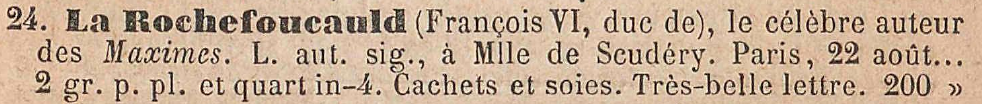
\includegraphics[width=\textwidth]{img/cat_000372_e24.png}
		\caption{Une lettre écrite par La Rochefoucauld vendue à 200 francs.}
		\label{fig:rochefoucauld}
	\end{subfigure}
	\begin{subfigure}{0.8\textwidth}
		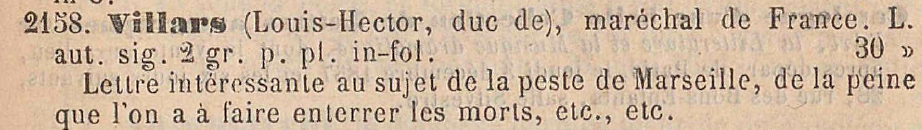
\includegraphics[width=\textwidth]{img/cat_000382_e2158.png}
		\caption{Une lettre écrite par Louis-Hector Villars vendue à 30 francs.}
		\label{fig:villars}
	\end{subfigure}
	\caption{Deux exemples de lettres}
\end{figure}

Pour analyser efficacement la variable \enquote{prix}, il faut pourtant pouvoir, dans une certaine mesure, comprendre les informations implicites et qualitatives contenues dans les catalogues. Le parti pris a donc été de construire le socle de connaissance qui manque à une machine, en s'alignant avec \wkd{} et en s'en servant pour enrichir nos données. Le choix a été fait de ne s'aligner avec \wkd{} que pour certaines parties des entrées de catalogue. Pour rappel, voici leur structure (\ref{code:tei_item}):

\begin{listing}
	\inputminted[linenos, breaklines, tabsize=4]{xml}{code/tei_item.xml}
	\caption{Représentation \xmltei{} d'une entrée de catalogue}
	\label{code:tei_item}
\end{listing}

Les entrées de catalogue contiennent beaucoup d'informations qualitatives, qui pourraient avoir une influence sur le prix du manuscrit: ici par exemple, la description du contenu de la lettre dans le \tnote{}; il est également souvent fait mention du ou de la destinataire. Cependant, l'alignement avec \wkd{} n'a pas été fait avec l'intégralité des entrées, mais seulement le contenu du \tname{}. Le \tdesc{} a déjà fait l'objet d'un grand travail de normalisation et d'extraction d'informations; un alignement avec des sources externes n'aurait donc pas une très grande plus-value. L'élément \tnote{} contient souvent des informations intéressantes, puisque c'est là qu'est décrit le contenu d'un manuscrit. Cependant, cet élément n'est pas toujours présent; son contenu est souvent écrit en langage naturel, non structuré, et contient des informations trop variées pour développer un traitement uniforme. Il est donc difficile de tirer parti de cet élément. Le \tname{} et son \ttrait{} sont les éléments les plus régulièrement présents; les informations qu'ils contiennent sont toujours les mêmes (nom d'une personne ou thème d'un manuscrit dans le \tname{}, description du \tname{} dans le \ttrait{}); enfin, ces deux éléments n'ont pas du tout été transformés dans le reste de la chaîne de traitement. Ils portent donc des informations qualitatives centrales pour produire des données exploitables dans une étude économétrique.

Le parti pris a donc été d'aligner avec des identifiants \wkd{} les noms contenus dans les balises \tname{} à l'aide des descriptions contenues dans les \ttrait{}; à partir de cet alignement a été constituée une base de données. Cela permet d'approximer une lecture \enquote{humaine} des items en vente: pour chaque auteur.ice, un certain nombre d'informations auront été récupérées pour mieux identifier la personne (ses occupations, son origine, ses dates de vie...). L'analyse du corpus s'appuie alors sur un bagage de connaissances qui permet d'appréhender par lecture distante l'importance d'une personne. Il devient alors envisageable de voir dans quelle mesure la mention d'une personne impacte le prix d'un manuscrit, et quels sont les facteurs biographiques déterminant dans l'établissement de la valeur. Pour revenir à l'exemple de La Rochefoucauld: à défaut de permettre de savoir qui il est, un alignement avec \wkd{} permet de mieux situer son statut et sa place dans la culture française, en récupérant le nombre de ses publications ou encore les institutions dont il est membre.

\subsection{Pourquoi utiliser la base de connaissances \wkd{}?}
De nombreuses bases de connaissances sont accessibles en ligne; celles-ci ont pour rôle de stocker et de diffuser des données structurées. Dans le paysage de la diffusion d'information sur le Web, les bases de connaissance s'opposent dont à de nombreux projets qui diffusent du texte, comme l'encyclopédie \wkd{}. Elles s'opposent également aux \enquote{dumps} de données, c'est-à-dire à la diffusion de jeux de données publics sur le Web. Les \enquote{dumps} -- tels qu'ils sont pratiqués par \href{https://www.data.gouv.fr/fr/}{\textit{Data.gouv}}, structure développée par la France -- sont des jeux de données \enquote{inertes}: les données sont diffusées dans des fichiers qui, une fois diffusés, ne seront pas mis à jour. Ces bases de connaissances donnent accès à de l'information brute, directement exploitable; les informations y sont accessibles individuellement et directement sur le Web (alors qu'elles sont contenues dans de lourds fichiers qui doivent être téléchargés dans le cas des \enquote{dumps}). Certaines de ces bases de connaissances ont été créées par des institutions publiques, comme \href{https://data.bnf.fr/}{\textit{DataBnF}}, créée par la Bibliothèque nationale de France. D'autres ont des sources universitaires, comme \href{https://www.dbpedia.org/}{\textit{DBPedia}} ou communautaires, c'est-à-dire qu'elles sont enrichies par une communauté d'utilisateur.ice.s -- dont certains peuvent être des acteurs institutionnels. Enfin, certaines de ces bases de connaissances sont spécialistes, comme le \href{https://thesaurus.inha.fr/thesaurus/}{Thésaurus INHA}, qui met à disposition du public les vocabulaires contrôlés développés par l'Institut d'histoire de l'art; d'autres, comme \textit{DBPedia}, sont généralistes. Un paysage varié -- brièvement présenté ici -- de solutions existent donc pour récupérer des données. Parmi cette variété de sources, laquelle choisir? Cette question fait l'objet de nombreuses études, notamment issues du domaine du traitement automatisé du langage\footcite{brando_evaluation_2016}. Des algorithmes complexes ont été développés pour juger de la qualité des données et de leur adaptation aux corpus d'un projet de recherche. L'utilisation de tels algorithmes ne s'intègre pas dans les méthodes du projet \ktb{}: ces algorithmes sont faits pour ensuite aligner les documents sources avec une base de connaissance à l'aide de méthodes d'apprentissage machine. Le projet \mssktb{} évite, lorsque cela est possible d'utiliser de tels outils. Une chaîne de traitement pour l'alignement avec \wkd{} a de plus déjà été élaborée; il n'était pas pertinent de modifier toute la chaîne de traitement simplement pour déterminer si une meilleure base de connaissance pourrait être utilisée.

La sélection de la base de connaissance à utiliser a donc été faite à partir d'une évaluation des besoins du projet. D'un point de vue des données, il était nécessaire d'utiliser une base généraliste, disposant d'informations biographiques sur des personnes et de données pertinentes pour un corpus issu de la France métropolitaine du \scl{XIX}. D'un point de vue technique, la base de connaissance devait disposer de deux outils. D'abord, l'alignement des \tname{} avec des entités \wkd{} devait être fait à l'aide de recherches en plein texte sur le moteur de recherche de la base; pour automatiser ce processus, la base de connaissance devait donc disposer d'une \api{} qui permette une telle opération. Ensuite, la constitution d'une base de donnée sur ces entités devait être faite à l'aide du langage de requêtes \sparql{}, qui permet la récupération automatisée d'informations structurées sur une base de données en ligne. \wkd{} répond à ces deux conditions. Mais cette base de donnée communautaire, développée par la \textit{Wikimedia Foundation} (également à l'origine de \textit{Wikipédia}) et rendue publique en 2012 présente de nombreux autres avantages. Contrairement à \textit{DBPedia}\footcite[p. 1]{muller-birn_peer-production_2015}, les données de \wkd{} sont directement produites par les contributeur.ice.s. Le projet est bicéphale, composé d'un côté de l'ajout d'informations à destination du public, et de l'autre de la construction d'une \gls{ontologie}; la particularité de \wkd{} est que les deux aspects sont collaboratifs, alors qu'en général, la construction d'une ontologie est le fait d'ingénieur.e.s professionel.le.s\footcite[p. 2-3]{muller-birn_peer-production_2015}. En 2015, la communauté \wkd{} représente 300000 personnes et 160 \textit{bots} (des programmes informatiques qui ajoutent automatiquement des données sur \wkd{})\footcite[p. 4]{muller-birn_peer-production_2015}. Cette communauté est basée sur une forme de division du travail entre humain.e.s et machines: 85\% des ajouts sont faits par des \textit{bots}, mais ce sont des ajouts simples et automatisables (par exemple, l'ajout d'identifiants uniques pour lier les entités à d'autres sources de données). La part humaine des contributions est consacrée aux ajouts plus complexes, avec une minorité d'acteur.ice.s (30\%) qui réalisent la très grande majorité des éditions, et sur de nombreux projets. À l'inverse, Les 70\% restants ont une contribution bien plus faible, et centrée sur un ou quelques sujets de prédilection. L'immense majorité des éditions représente des ajouts d'informations, tandis que l'évolution de la structure de \wkd{} repose sur une poignée d'utilisateur.ice.s très spécialisé.e.s\footcite[p. 4, 8-9]{muller-birn_peer-production_2015}. Rien que par son envergure et la quantité de données disponibles, \wkd{} est un candidat intéressant pour le projet d'alignement des \tname{} avec une base de connaissances externe. Par ailleurs, sa nature généraliste s'adapte à la vaste période couverte par le corpus, ainsi qu'à la variété d'informations qui peuvent être contenues dans le \tname{}. La nature communautaire du projet est elle aussi intéressante: \wkd{} est enrichi par une communauté internationale, et de nombreuses données sont donc disponibles pour un corpus français; des bases non-communautaires risquent toujours d'avoir un biais national dans les données disponibles.

Le modèle de données et les choix techniques pour leur ingénierie font de \wkd{} une source adaptée aux objectifs du projet \ktb{}. Tous les objets qui sont documentés par \wkd{} (appelés entités) peuvent être classés en deux types\footcite[p. 51-52]{mika_introducing_2014}: 

\begin{itemize}
	\item Les items, c'est-à-dire des données sur laquelle d'autres informations sont disponibles. Ceux-ci correspondent à des choses physiques ou à des concepts du monde réel, et peuvent être classifiés en deux catégories: les classes et les individus. Les classes sont des catégories génériques (\enquote{une personne}) tandis que les individus sont des membres de ces catégories (\enquote{Natalia Gontcharova}).
	\item Les propriétés, qui caractérisent les relations entre un ou plusieurs items. Par exemple, \enquote{occupation} permettrait de lier l'item \enquote{Natalia Gontcharova} à l'item \enquote{peintre}.
\end{itemize}

D'un point de vue technique, ce modèle est intéressant: il correspond à l'organisation des données du Web sémantique et de \sparql{}\footcite[p. 51-52]{mika_introducing_2014}; cela facilite l'utilisation ultérieure de ce langage de requêtes (décrite plus base): la relation entre les données, qui est utilisée pour récupérer des informations avec \sparql{}, est explicite; il est donc facile de trouver comment structurer des requêtes. Là encore en concordance avec les modèles de données sémantiques, chaque item dispose d'un identifiant unique, d'un \gls{uri}; c'est ces identifiants qui sont utilisés dans \sparql{} pour récupérer des données, ce qui facilite encore l'utilisation de ce langage\footcite[p. 56]{mika_introducing_2014}. Enfin, une dernière spécificité de cette base de connaissances est intéressante en vue de l'utilisation ultérieure de \sparql{}: \wkd{} a fait le choix de n'utiliser qu'un vocabulaire par catégorie de données. Comme nous le verrons plus tard, dans le Web sémantique, un vocabulaire est nécessaire pour définir les propriétés reliant plusieurs entités; par exemple, un identifiant est relié à son nom grâce à la propriété \enquote{\texttt{rdfs:label}}, qui appartient au vocabulaire \texttt{rdfs}. Ces vocabulaires doivent être utilisés avec \sparql{}. Plusieurs vocabulaires ont souvent leurs propres manières de définir les mêmes relations, et les bases de connaissance ont tendance à utiliser plusieurs vocabulaires qui se chevauchent -- c'est par exemple le cas de \textit{DataBnF}. Cela rend le modèle de données utilisés par ces bases particulièrement complexe; il est donc difficile de naviguer dedans, et encore plus difficile de récupérer des données via \sparql{}. À l'inverse, la majorité des propriétés sont définies par l'ontologie de \wkd{}, qui est très bien documenté sur le site; cela rend la manipulation des données sur cette base de connaissances particulièrement aisée. Ainsi, \wkd{} dispose d'un modèle de donnée totalement adapté à l'utilisation de langages de requêtes dédiées aux modèles de données sémantiques.

Dans \wkd{}, tout item contient les mêmes types informations. Trois sont particulièrement intéressantes pour le processus d'alignement: le label, la description et les alias\footcite[p. 52]{mika_introducing_2014}. Un label permet de nommer un item; par conséquent, il est possible de distinguer l'entité (représentée par un identifiant normalisé) et sa représentation linguistique (le label). Cette distance est intéressante pour le projet \ktb{}: l'alignement des \tname{} avec des entités \wkd{} revient retrouver un identifiant à partir du label qui lui est associé. Ce label est unique; cependant, il existe de nombreux alias, qui sont des représentations linguistiques multilingues ou des variations du nom associé à une entité. Cela veut dire que, même si, dans un catalogue, un.e auteur.ice n'est pas nommé.e de façon canonique (en traduisant son nom, par exemple), il est toujours possible d'aligner le \tname{} avec une entité \wkd{} à l'aide des alias. La description, enfin, contient souvent la date de naissance et de décès ainsi que l'occupation d'une personne; autant d'informations qui sont contenues dans le \ttrait{} et qui seront donc utilisées dans le processus d'alignement. De l'expérience que j'ai pu en faire, label, alias et description sont indexés par le moteur de recherche de \wkd{}: cela veut dire que en recherchant ces informations sur l'\api{}, les données des catalogues pourront être alignées avec les entités pertinentes.

Pour toutes ces raisons, la base de connaissance pour le processus d'alignement avec une source de données externe est \wkd{}. Cette plateforme dispose à la fois des outils techniques nécessaires, d'un socle de données correspondant à l'univers de discours du corpus et d'une certaine facilité d'utilisation, un critère non négligeable pour garantir la réutilisation ultérieure des processus développés.

\subsection{Quelle relation avec la résolution d'entités nommées d'entités nommées?}
En traitement automatisé du langage, le processus d'alignement d'éléments d'un texte avec une base de connaissances externe a un nom: c'est la résolution d'entités nommées (plus tard abrégée sous son acronyme anglo-saxon, \gls{nel}). Pour reprendre la définition proposée par Brando et al.: \enquote{La tâche dite de résolution d’entités nommées [...] consiste à affecter automatiquement la bonne référence, l’identifiant de la ressource correspondante dans une base de connaissances ou bien NIL (l’absence de valeur), à une entité nommée préalablement identifiée dans un texte et étiquetée.}\footcite[p. 31]{brando_evaluation_2016}. Dans un texte, ce processus arrive après l'identification dans un texte d'entités, c'est-à-dire d'objets uniques et signifiants pour une problématique de recherche: personnes, lieux, mais aussi parfois concepts. Il consiste à aligner les entités du texte avec celles présentes sur une base de connaissance externe. Deux objectifs primaires peuvent être identifiés\footcite[p. 32]{brando_evaluation_2016}. Le premier est la désambiguïsation des entités dans un texte, ce qui permet à une machine de ne pas confondre deux entités homonymes (Alexandre Dumas père et fils, par exemple). Cette étape est très importante pour le traitement automatisé d'un texte: si un.e lecteur.ice humain.e est capable de distinguer les deux Alexandre Dumas en fonction de sa lecture et de ses références, cette distinction est impossible par une machine. La reconnaissance d'entités nommées permet alors d'expliciter l'implicite, ce qui est également l'un des objectifs ayant mené à l'alignement des auteur.ice.s de catalogues avec des entités de \wkd{}. Le deuxième objectif est \enquote{l'enrichissement sémantique}, c'est-à-dire la récupération d'informations depuis une source externe pour permettre une meilleure compréhension et analyse du texte par des méthodes computationnelles. Comme cela a été dit plus haut, c'est exactement à cette fin qu'est mené l'alignement des \tname{} avec \wkd{}. Pourquoi alors ne pas directement parler d'un processus de résolution d'entités nommées?

Tout d'abord, l'alignement avec \wkd{} n'était pas censé prendre une telle ampleur à ses débuts. Il avait initialement été prévu de réaliser cet alignement \enquote{à la main}, ce qui, pour un corpus de près de 100000 entrées, aurait été extrêmement chronophage. C'est avant tout pour répondre à ce problème purement pratique qu'ont été développées des méthodes pour automatiser l'alignement qui sont présentées ici. Étant donné que les entrées sont riches d'informations, il est apparu que ce processus pouvait être réalisé automatiquement, avec bien sûr un certain degré d'erreur. En choisissant d'automatiser l'alignement, les méthodes d'extraction d'informations des catalogues et de recherches sur l'\api{} se sont progressivement complexifiées afin de mieux s'adapter au corpus. L'alignement avec \wkd{} a donc progressivement été développé, jusqu'à devenir un processus analogue à la résolution d'entités nommées.

Ensuite et surtout, la résolution d'entités nommées \enquote{traditionnelle} implique des méthodes en tout point différentes de celles qui sont présentées ici. Le \gls{nel} repose très fortement sur l'apprentissage machine. Il est d'abord utilisé pour identifier les entités dans le texte\footcite[p. 32]{brando_evaluation_2016}; ensuite, il sert à mener l'alignement des entités avec la base de connaissances elle-même. Pour ce processus, de nombreux outils ont été développés, comme \texttt{REDEN}\footcite{brando_reden_2016} ou \texttt{DBpediaSpotlight}\footcite{mendes_dbpedia_2011}, conçu au sein du projet \textit{DBPedia} pour la résolution d'entités en utilisant cette base de connaissance. Ces outils fonctionnent, d'une certaine manière, à l'inverse du processus mis en place ici: à partir d'un ensemble de références potentielles récupérées d'une base de connaissance à l'aide de requêtes \sparql{}\footcite[p. 35]{brando_evaluation_2016} avant d'extraire une liste de candidats potentiels pour la résolution d'entités, puis de résoudre l'entité en y assignant un item issu de la base de connaissance\footcite[p. 33]{brando_evaluation_2016}, À l'inverse, le processus mis en place ici consiste d'abord à extraire des données des textes, ensuite d'interagir avec un moteur de recherche pour sélectionner une entité parmi toutes celles disponibles sur la base de connaissances, et enfin de mener des requêtes \sparql{} pour récupérer des données supplémentaires sur les items liés. Dans le détail, les méthodes utilisées pour la résolution d'entités sont également très différentes: elles se basent, de manière générale, sur une tentative d'aligner l'entité du texte avec une entité sur la base de connaissance par l'analyse de graphes\footcite[p. 63]{brando_reden_2016}. Pour ce faire, les entités de la base sont représentées sous forme de graphes qui sont analysés pour trouver, au sein du graphe, l'entité pertinente; l'apprentissage machine permet à un outil \enquote{d'apprendre} à reproduire tout seul ce processus d'analyse du graphe, afin d'aligner d'autres entités avec leur équivalent sur une base de connaissances. Dans le processus décrit ici, il n'y a ni analyse de graphes, ni apprentissage machine: l'alignement se base sur la détection de motifs à l'aide d'\glspl{expression régulière}. Des informations sont détectées dans les catalogues, extraites et si besoin retraitées, avant d'être utilisées pour faire des recherches sur \wkd{} afin d'aligner un.e auteur.ice avec une entité de cette base de connaissances. Le processus décrit ici privilégie donc une compréhension approfondie du corpus, de sa structure et de son vocabulaire, ainsi qu'une bonne connaissance du fonctionnement du moteur de recherche de \wkd{}. Si les méthodes sont radicalement différentes, les possibilités ouvertes sont équivalentes. Les scores de performance des deux méthodes sont, comme nous le verrons, relativement proches, ce qui ouvre à la possibilité de chercher à développer des méthodes alternatives pour la résolution d'entités nommées.

\section{Questions de méthode: comment faire le lien entre un corpus historique et une base de connaissances en ligne?}
\sectionmark{Questions de méthode}
\subsection{Présentation générale de l'algorithme}
Construire un jeu de données issu de \sparql{} à partir de la manière dont une personne est nommée et décrite au \scl{XIX} n'est pas une opération anodine. La chaîne de traitement est donc assez complexe, comme le montre le schéma \ref{fig:wkdmain}. Cette chaîne de traitement peut être séparée en trois étapes.

\subsubsection{Étape 1 -- Extraction et structuration de données}
Premièrement, il s'agit d'aligner les entrées de catalogue avec des identifiants \wkd{}. Ceux-ci sont liés à des entités \wkd{}. Cette première étape repose avant tout sur l'extraction et la traduction des données depuis les éléments \tname{} et \ttrait{}. Ce processus d'extraction permet de récupérer toutes les données pertinentes pour chaque entrée de catalogue et de les stocker dans un \gls{dictionnaire} structuré. Comme on le verra, la nature \enquote{semi-structurée} des entrées (ainsi qu'une bonne connaissance du corpus) permet de d'automatiser le processus d'extraction et de traduction des données par détection de motifs, sans avoir à passer par l'apprentissage machine: étant donné que les mêmes types d'informations sont toujours présentes et que les entrées suivent des modèles relativement proches, il est possible de s'appuyer sur la structure des entrées pour identifier  les informations pertinentes. L'extraction de données repose donc sur de la détection de motifs à l'aide d'\rgxpl{}: des récurrences sont repérées dans le texte et utilisées pour distinguer différentes informations (nom, prénom, titre de noblesse...). Pour appuyer l'usage d'expressions régulières par une méthode plus \enquote{qualitative} et précise, certains termes particuliers sont extraits et éventuellement traduits à l'aide de \glspl{table de conversion} (c'est-à-dire de \glspl{dictionnaire} qui associent à un terme dans le texte une version normalisée). 

\subsubsection{Étape 2 -- récupération d'identifiants \wkd{} via des recherches en plein texte à l'aide d'une \api{}}
Une fois les données du \tname{} et du \ttrait{} structurées en dictionnaire, elles sont utilisées pour lancer plusieurs recherches en plein texte sur le moteur de recherche de \wkd{}. Ces recherches sont faites automatiquement grâce à l'\api{} de \wkd{}. Pour maximiser les chances d'obtenir un identifiant valide, un algorithme a été conçu pour lancer plusieurs recherches à partir de chaque entrée. La première recherche met bout-à-bout toutes les valeurs disponibles dans le dictionnaire. Ensuite, en fonction des paramètres de recherche disponibles dans le dictionnaire, différentes autres recherches sont lancées. Cet algorithme a été élaboré en menant de nombreux tests pour maximiser le taux de réussite, calculé sous la forme d'un \gls{score F1}.

\subsubsection{Étape 3 -- constitution d'un jeu de données à l'aide de \sparql{}}
Si l'étape d'alignement avec \wkd{} est la plus complexe, elle n'est qu'une étape préparatoire vers la constitution du jeu de données et à l'enrichissement sémantique. En fait, résoudre les entités est ce qui rend possible l'enrichissement en tant que tel: en lançant une requête \sparql{} sur tous les identifiants obtenus, il est possible de récupérer des informations depuis \wkd{} et donc de construire le jeu de données définitif. Pour cette étape, le processus est plus simple: les identifiants récupérés à la fin de l'étape précédente sont dédoublonnés (pour éviter de lancer plusieurs fois la même requête); ensuite une requête \sparql{} est initalisée et lancée chacun des identifiants. Les résultats sont traduits depuis les formats \json{} ou \xml{} retournés par \sparql{} sous forme de \json{} plus simple, et donc plus aisément manipulable. Le jeu de données est enregistré dans un fichier. Pour finir, les identifiants \wkd{} sont réinjectés aux catalogues \tei{}, afin de pouvoir faire le lien entre les documents et le jeu de données qui a été construit.

Cette chaîne de traitement étant lancée sur plus de 80000 entrées de catalogues, le temps d'exécution est très long et même des petites améliorations de performance peuvent avoir un grand impact; dans sa version initiale, le script demandait des performances particulièrement élevées, et ne fonctionnait pas sur un ordinateur de bureau. La chaîne de traitement a donc été reprise en plusieurs points afin d'être optimisée, de fonctionner plus vite en étant moins coûteuse en ressources.

\widepage
\begin{figure}[!p]
	\centering
	\tikz[node distance=1cm, scale=0.85, transform shape]{
		\node[db] %
		(db1) at (-5,0)%
		{Source: tableur contenant les \tname{} et \titem{}};
		\node[base]%
		(start) at (0,0)%
		{Lancement de l'algorithme sur toutes les entrées du tableur};
		\draw[arrow] (db1) -- (start);
		
		\node[choice]%
		(detect) at (0,-3.5)%
		{Étape 1 -- extraction de donnée des \tname{} et \ttrait{}};
		\draw[arrow] (start) -- (detect);
		
		\node[transf]%
		(name) at (-4,-6.5)%
		{Extraction et normalisation d'informations nominatives du \tname{}};
		\node[transf]%
		(trait) at (4,-6.5)%
		{Extraction et normalisation d'informations biographiques du \ttrait{}};
		\node[base]%
		(dict) at (0,-9.5)%
		{Constitution d'un dictionnaire structuré pour aligner les \tname{} avec des entités \wkd{}};
		\draw[arrow] (detect) -- (name);
		\draw[arrow] (detect) -- (trait);
		\draw[arrow] (name) -- (dict);
		\draw[arrow] (trait) -- (dict);
		
		\node[db]%
		(logs) at (6,-13)%
		{Optimisation: enregistrement des entrées de catalogues et requêtes déjà traitées};
		\node[transf]%
		(api) at (0,-13)%
		{Étape 2 -- Alogrithme de requêtes sur l'API \wkd{} pour récupérer des identifiants};
		\draw[arrow] (api) -- (logs);
		\draw[arrow] (dict) -- (api);
		
		\node[db]%
		(idset) at (0,-17.5)%
		{Liste d'identifiants \wkd{} à partir de laquelle est constitué le jeu de données};
		\node[transf]
		(sparql) at (0,-20.5)
		{Étape 3 -- Requêtes \sparql{}};
		\node[base]%
		(end) at (0, -23)%
		{Conversion des résultats en \json{} et enregistrement};
		\node[db]%
		(sparqldata) at (5,-23)%
		{Jeu de données issues de \sparql{} au format \json{}};
		\node[transf]%
		(tei) at (0,-25.5)%
		{Réinjection des identifiants \wkd{} dans les fichiers \tei{}};
		\node[db]%
		(teidb) at (-5,-25.5)%
		{Corpus de catalogues en \tei{} augmentés des identifiants \wkd{}};
		\draw[arrow] (api) -- (idset);
		\draw[arrow] (idset) -- (sparql);
		\draw[arrow] (sparql) -- (end);
		\draw[arrow] (end) -- (sparqldata);
		\draw[arrow] (end) -- (tei);
		\draw[arrow] (tei) -- (teidb);
	}
	\caption{\\Présentation générale de l'algorithme d'enrichissement de données à l'aide de \wkd{}}
	\label{fig:wkdmain}
\end{figure}
\restoregeometry

\subsection{Comment traduire des descriptions textuelles datant du XIX\up{ème}~s. en chaînes de caractères pouvant retourner un résultat sur \wkd{}?} 
Dans la réalisation de cet algorithme, la principale difficulté porte sur la récupération d'identifiants \wkd{} à l'aide de recherches en plein texte. Le script prend en entrée un nom et sa description -- tels qu'elles figurent dans des catalogues datant majoritairement du \scl{XIX}. La difficulté, au delà de la détection et de l'extraction d'informations, est de traduire ces informations pour qu'elles permettent de trouver des résultats pertinents sur \wkd{}. Ce problème est autant linguistique de technique. Une personne ou une chose est nommée ou décrite d'une certaine manière dans un catalogue de vente ancien. Il n'y a aucune garantie que cette caractérisation corresponde à celle faite par \wkd{}: l'orthographe des noms évoluent, tout comme la manière de nommer certains métiers. À ces évolutions orthographiques s'ajoutent des évolutions intellectuelles: les titres de noblesse sont un marqueur plus important au \scl{XIX} français que dans un \scl{XXI} mondialisé. Une personne n'est que rarement décrite par son titre dans \wkd{}. 

\subsubsection{Le problème de la traduction des noms}
Il existe bien sûr des cas simples, comme l'exemple \ref{code:name1}: en extrayant le contenu du \tname et en traduisant le \enquote{roi} issu du \ttrait{}, la chaîne de caractère obtenue est \enquote{Henri IV king}. En recherchant cette chaîne de caractère sur \wkd{}, \href{https://www.wikidata.org/w/index.php?search=Henri+IV+king\&title=Special:Search\&profile=advanced\&fulltext=1\&ns0=1\&ns120=1}{le premier résultat obtenu est correct}. Cependant, de nombreux cas sont plus complexes, surtout lorsque l'auteur.ice du manuscrit est moins célèbre. L'exemple \ref{code:name2} est éclairant: dans le catalogue, la personne est nomée \enquote{Bruno Daru}; sur \wkd{}, le nom de la personne est \enquote{Pierre Daru}, et son nom complet {Pierre Antoine Noël Bruno Daru}. Si la recherche en plein texte est faite avec les mêmes paramètres que pour l'exemple précédent (nom de la personne et titre de noblesse), \href{https://www.wikidata.org/w/index.php?search=bruno+daru+count&title=Special:Search&profile=advanced&fulltext=1&ns0=1&ns120=1}{le premier résultat obtenu} n'est pas le bon: c'est un renvoi à un article de \textit{l'Encyclopedia Britannica} datant de 1911. C'est en cherchant seulement le nom est le prénom que \wkd{} retourne \href{https://www.wikidata.org/w/index.php?search=bruno+daru&title=Special:Search&profile=advanced&fulltext=1&ns0=1&ns120=1}{un résultat pertinent}. Deux choses sont à retenir de cet exemple: dans les catalogues, le prénom d'une personne correspond en fait souvent à son deuxième ou troisième prénom; ensuite, le titre de noblesse est un critère plus fréquemment mentionné dans les catalogues que dans \wkd{}. Cela s'explique assez aisément: le \scl{XIX} connaît une alternance de régimes politiques (royauté, empire, république) où la noblesse n'a pas encore perdu son pouvoir. La probabilité qu'un titre de noblesse soit mentionné sur \wkd{} diminue lorsqu'un titre est peu important; dans les catalogues, cependant, même les titres les moins importants sont régulièrement mentionnés. Par conséquent, seuls les titres les plus importants seront extraits pour faire des recherches sur \wkd{}.

\begin{listing}
	\begin{minted}{xml}
<item n="134" xml:id="CAT_000233_e134">
	<!-- ... -->
	<name type="author">Henri IV</name>
	<trait>
		<p>roi de France.</p>
	</trait>
	<!-- ... -->
</item>
	\end{minted}
	\caption{Un cas simple: Henri IV roi de France}
	\label{code:name1}
\end{listing}

\begin{listing}
	\begin{minted}{xml}
<item n="98" xml:id="CAT_000082_e98">
	<!-- ... -->
	<name type="author">Daru (Bruno, comte)</name>
	<trait>
		<p>célèbre ministre de Napoléon Ier, historien de Venise, de l'Acad. fr., né à Montpellier</p>
	</trait>
	<!-- ... -->
</item>
	\end{minted}
	\caption{Un cas plus complexe: Pierre Antoine Noël Bruno Daru}
	\label{code:name2}
\end{listing}

Dans le cas de noms de personnes étrangères, la situation peut être plus complexe encore. L'exemple \ref{code:name3} combine différentes difficultés.
\begin{itemize}
	\item D'abord, la personne est étrangère; dans les catalogues, les noms sont systématiquement françisés -- \enquote{Albert-Venceslas-Eusèbe} dans le catalogue, \enquote{Albrecht Wenzel Eusebius} en langue originelle. Se pose donc la question de si le nom doit être traduit, et si oui comment? 
	\item Ensuite, comme l'indique la présence de \enquote{dit} dans le \tname{}, il est mentionné un nom de naissance (\enquote{de Waldstein}) et un nom d'usage (\enquote{Wallenstein}). Idéalement, il faudrait choisir entre l'un ou l'autre, plutôt que de rechercher \enquote{Waldstein Wallenstein} sur \wkd{}, ce qui risque d'augmenter le bruit. 
\end{itemize}

Notre approche s'appuyant sur la structure du texte, le deuxième point peut être réglé: le nom d'usage est écrit au début, et le nom de naissance entre parenthèses (c'est également le cas des noms de personnes nobles, par exemple). Il est donc possible de choisir l'un ou l'autre nom. Le premier point est plus problématique: si la traduction du nom serait envisageable en théorie, celle-ci est difficilement compatible avec une approche basée sur la détection de motifs dans le texte: un prénom est repérable comme étant un motif (trois noms séparés par des tirets); cependant, il est impossible de le traduire automatiquement (ce qui demanderait de connaître la langue dans laquelle un prénom doit être traduit). C'est ici que les informations contenues dans le \ttrait{} prennent leur importance: lorsqu'il y a des défaillances dans les informations nominatives, des données biographiques permettent de diminuer le risque d'erreurs. Dans cet exemple, recherche \enquote{Albert-Venceslas-Eusèbe Waldstein} ne \href{https://www.wikidata.org/w/index.php?search=Albert-Venceslas-Eus%C3%A8be+de+Waldstein&title=Special:Search&profile=advanced&fulltext=1&ns0=1&ns120=1}{retourne aucun résultat}, de même que rechercher \href{https://www.wikidata.org/w/index.php?search=Albert-Venceslas-Eus%C3%A8be+Wallenstein&title=Special:Search&profile=advanced&fulltext=1&ns0=1&ns120=1}{Albert-Venceslas-Eusèbe Wallenstein}. Cependant, le bon résultat est obtenu en recherchant \href{https://www.wikidata.org/w/index.php?search=Wallenstein+1634&title=Special:Search&profile=advanced&fulltext=1&ns0=1&ns120=1}{\enquote{Wallenstein 1634}}. Une difficulté supplémentaire vient avec ce type de cas: différents paramètres de recherche (nom, prénom...) ont un impact différent dans l'obtention du bon résultat en fonction des personnes sur qui la requête est faite. Dans ce cas, rechercher le nom d'usage et la date de naissance retourne un résultat valide, ce qui n'est pas toujours le cas. Pour contourner ce problème, trois solutions ont été mises en place: d'abord, ce types de requêtes a été fait \enquote{à la main}, de façon non-automatique, pour de nombreuses entrées différentes afin de déterminer la meilleure combinaison de caractères; ensuite, des tests qui permettent de mesurer l'influence de chaque paramètre de recherche dans l'obtention du résultat ont été réalisés; enfin, l'algorithme final lance successivement différentes requêtes avec différents paramètres afin de maximiser la probabilité d'obtenir un résultat valide. Nous reviendrons plus en détail sur les deux derniers points.

\begin{listing}
	\begin{minted}{xml}
<item n="5518" xml:id="CAT_000401_e5518">
	<!-- ... -->
	<name type="author">Wallenstein (Albert-Venceslas-Eusèbe de Waldstein  dit)</name>
	<trait>
		<p>duc de Friedland, célèbre général de la guerre de Trente ans. Assassiné en 1634.</p>
	</trait>
	<!-- ... -->
</item>
	\end{minted}
	\caption{Le problème des noms de personnes étrangères}
	\label{code:name3}
\end{listing}

\subsubsection{L'extraction d'informations biographiques: une autre difficulté}
Cependant, le problème ne s'arrête pas qu'aux noms. Dans un exemple; précédent, le titre de noblesse influençait l'obtention d'un résultat valide. De nombreuses autres informations biographiques pourraient, au premier abord, permettre d'obtenir le bon résultat. C'est souvent le cas, puisque extraire le métier ou la fonction d'une personne permet de supprimer les faux positifs retournés par l'\api{}. C'est par exemple le cas dans l'exemple \ref{code:bio1}. En cherchant uniquement le nom et le prénom (\enquote{Hans Bulow}), le premier résultat retourné renvoie \href{https://www.wikidata.org/w/index.php?search=hans+bulow&title=Special:Search&profile=advanced&fulltext=1&ns0=1&ns120=1}{à un journaliste suédois}. Extraire le mot \enquote{pianiste} \ttrait{} et le traduit en anglais permet d'obtenir \href{https://www.wikidata.org/w/index.php?search=hans+bulow+pianist&title=Special:Search&profile=advanced&fulltext=1&ns0=1&ns120=1}{le bon résultat}.

\begin{listing}
	\begin{minted}{xml}
<item n="136" xml:id="CAT_000189_e136">
	<!-- .. -->
	<name type="author">Bulow (Hans)</name>
	<trait>
		<p>le célèbre pianiste.</p>
	</trait>
</item>
	\end{minted}
	\caption{Un exemple où l'extraction du métier permet l'obtention du bon résultat}
	\label{code:bio1}
\end{listing}

L'extraction d'informations biographiques et leur utilisation dans des requêtes est donc pertinent. Cependant, extraire trop d'informations conduit à lancer des requêtes qui ne renvoient aucun résultat. Dans les exemples \ref{code:bio2} et \ref{code:bio3}, extraire et traduire des fonctions conduit à lancer les requêtes \href{https://www.wikidata.org/w/index.php?search=John+Okey+colonel&title=Special:Search&profile=advanced&fulltext=1&ns0=1&ns120=1}{\enquote{John Okey colonel}} et \href{https://www.wikidata.org/w/index.php?search=Jean+Bouhier+president&title=Special:Search&profile=advanced&fulltext=1&ns0=1&ns120=1}{\enquote{Jean Bouhier president}} qui ne retournent aucun résultat, ou des résultats qui ne sont pas valides. Cependant, dans les deux cas, si une requête est lancée sans le métier, un résultat correct est obtenu. Les raisons pour lesquelles des résultats erronés sont retournés ne sont cependant pas les mêmes, et il est intéressant de mieux observer les requêtes lancées et les résultats obtenus. Dans le premier cas, le terme mis en avant dans le \ttrait{} (\enquote{colonel}) n'est pas celui avec lequel la personne est décrite sur \wkd{} (où John Okey est décrit comme étant un homme politique). Cela met en avant un problème relatif au changement de regard sur des personnalités: dans un contexte, la personne est décrite comme une figure militaire, dans l'autre comme une figure politique. Le deuxième cas est plus technique. Il y a en fait une erreur dans la requête qui ne retourne pas de résultat (\enquote{Jean Bouhier president}): un.e président.e de parlement n'est en général pas décrite comme \enquote{président}. Cependant, en extrayant des données uniquement par détection de motifs, il est possible de repérer et traduire un terme générique comme \enquote{président}. Extraire le complément \enquote{Parlement de Dijon} du \ttrait{} n'est cependant pas possible (cela impliquerait d'étudier la grammaire de la phrase, pour mettre en avant la relation entre \enquote{président} et \enquote{Parlement de Dijon}). Au vu de la taille et de la variété du jeu de données, il est impossible de traiter au cas par cas des entrées, ou préciser suffisamment la détection de motifs pour pouvoir résoudre ce genre de difficultés. 

De situations comme les exemples \ref{code:bio2} et \ref{code:bio3}, il faut donc retenir que l'extraction d'informations vient nécessairement avec un risque d'erreur. Le parti pris a donc été de ne pas repérer les métiers et autres termes très spécifiques, comme les grades militaires et les titres de noblesse peu élevés: ils ne retournent pas de résultats sur le moteur de recherche. Ensuite, plus des requêtes sont précises, plus elles risquent de retourner du silence (c'est-à-dire, de ne pas donner de réponse); cependant, si un résultat est obtenu, il est plus probable que ce résultat soit correct. Une fois l'extraction d'informations faite, l'algorithme de résolution d'entités avec \wkd{} a donc été conçu en suivant un principe soustractif: les premières recherches sont faites avec un maximum de paramètres; si aucun résultat n'est obtenu, des paramètres sont enlevés pour que l'\api{} retourne un plus grand nombre de résultats. Enfin, ces deux exemples montrent qu'il n'est pas possible d'extraire et de traduire des informations sans prendre en compte ce qui sera pertinent pour le moteur de recherche de \wkd{}. Il ne s'agit donc pas seulement d'extraire des informations, mais aussi de s'adapter avec ce moteur de recherche pour augmenter la probabilité d'obtenir un résultat valide.

\begin{listing}
	\begin{minted}{xml}
<item n="152" xml:id="CAT_000189_e152">
	<!-- ... -->
	<name type="author">Okey (John)</name>
	<trait>
		<p>colonel anglais, un des lieutenants de Cromwell.</p>
	</trait>
	<!-- ... -->
</item>
	\end{minted}
	\caption{Quand l'extraction d'un métier conduit à des requêtes trop spécifiques}
	\label{code:bio2}
\end{listing}

\begin{listing}
	\begin{minted}{xml}
<item n="5430" xml:id="CAT_000401_e5430">
	<!-- ... -->
	<name type="author">Bouhier (Jean)</name>
	<trait>
		<p>président au Parlement de Dijon, membre de l'Académie française.</p>
	</trait>
	<!-- ... -->
</item>
	\end{minted}
	\caption{Le cas des métiers dont l'extraction est problématique}
	\label{code:bio3}
\end{listing}

\subsection{Comment négocier avec le moteur de recherche de \wkd{}?}
Comme cela commence à apparaître, l'extraction d'informations, lorsqu'elle vise à interagir avec des données externes, vient avec des difficultés supplémentaires. Il ne faut pas seulement extraire les informations ; leur extraction et structuration doivent permettre de lancer des recherches en plein texte, et donc de minimiser le bruit (les informations non pertinentes) et le silence (l'absence d'informations) de la part du moteur de recherche. Il faut donc traduire les informations extraites pour qu'elles correspondent au vocabulaire utilisé par \wkd{}. Cette opération n'est pas anodine: si les catalogues de vente fonctionnent avec leurs propres catégories, le même peut être dit de \wkd{}: certains types de données sont plus souvent référencées que d'autres et \wkd{} utilise un vocabulaire qui lui est propre. Pour bien mener ce processus de traduction et de structuration de l'information, il est nécessaire de bien connaître le fonctionnement de ce moteur de recherche pour mieux s'y adapter.

Comme cela a été dit, l'alignement avec \wkd{} passe par l'utilisation de l'\api{} mise en point par l'institution afin de lancer automatiquement des recherches en plein texte; l'objectif est que le premier résultat retourné par le moteur de recherche soit le bon. La première chose à remarquer est que, contrairement à un moteur de recherche généraliste (comme \textit{Google, QWant}...), ce moteur n'est pas compatible avec des requêtes approximatives. L'exemple \ref{code:search1} est pertinent à ce égard\footnote{Dans cet exemple, le prénom, \enquote{M.-D.-A.}, n'est pas pris en compte pour se concentrer sur l'utilisation d'informations biographiques dans le \ttrait{}.}. Dans de nombreuses entrées, comme c'est le cas ici, les fonctions d'une personne ayant participé à la révolution sont présentées de façon précise: Marc David Alba Lasource est décrit comme étant un \enquote{conventionnel girondin}. Cette mention, régulièrement présente dans les catalogues, pourrait être relevée en tant que telle. Cependant, lancer la recherche \enquote{Lasource conventionnel} ne retourne \href{https://www.wikidata.org/w/index.php?search=lasource+conventionnel&title=Special:Search&profile=advanced&fulltext=1&ns0=1&ns120=1}{aucun résultat}. Si la même recherche est lancée sur un moteur de recherche généraliste (ici, \textit{QWant}), la page \textit{Wikipedia} de Lasource fait partie des premiers \href{https://www.qwant.com/?q=lasource+conventionnel}{résultats}\footnote{Le 29/07/2022, c'est le troisième résultat; le premier correspond à une vente aux enchères d'archives du conventionnel. Les moteurs de recherche pouvant être mis à jour régulièrement, il est possible que l'ordre des résultats change}. Cette différence dans les données retournées par les moteurs de recherche a deux explications: un moteur de recherche généraliste recherche les occurrences de mots, non seulement dans le titre de la page, mais aussi dans le corps du texte. Si le mot \enquote{conventionnel} est absent du titre, il est certainement à plusieurs reprises dans une notice biographique type \textit{Wikipedia}. \wkd{} ne contenant que des données, et pas de texte en tant que tel, l'indexation du corps du texte par le moteur de recherche interne à \wkd{} n'est pas possible. Ensuite, la plupart des moteurs de recherche généralistes utilisent des méthodes de traitement du langage afin de simplifier la requête lancée par l'utilisateur.ice: les mots recherchés sont simplifiés, le moteur de recherche associe les termes recherchés avec d'autres termes \enquote{cooccurents}, c'est-à-dire fréquemment utilisés ensemble\footnote{\cite{noauthor_moteur_2022}. Pour des analyses plus détaillées sur la construction d'ensemble de termes coocurrents via le développement de vecteurs de mots, voir \cite{mikolov_efficient_2013}; pour un article technique détaillant la classification et la sélection de résultats pertinents par apprentissage profond, voir \cite{covington_deep_2016}}. Dans le cas du moteur de recherche de \wkd{}, la requête de l'utilisateur.ice ne semble pas être retraitée: des signes de ponctuation ou des fautes de frappes influencent l'obtention d'un résultat, de même que l'usage de termes inadaptés.

Pour faire face à la \enquote{rigidité} relative du moteur de recherche de \wkd{}, il est donc nécéssaire de préparer ses données au moment de leur extraction. En prenant le même exemple (\ref{code:search1}), un résultat correct peut être obtenu en remplaçant \enquote{conventionnel} par \enquote{politician}\footnote{\enquote{Personnalité politique}}, pour rechercher sur \wkd{} \href{https://www.wikidata.org/w/index.php?search=lasource+politician&search=lasource+politician&title=Special%3ASearch&go=Go&ns0=1&ns120=1}{\enquote{Lasource politician}}. Ici, la traduction de \enquote{conventionnel} en \enquote{politician} est d'autant plus intéressante que la date de naissance dans le catalogue (1762) ne correspond pas à celle indiquée sur \wkd{} (1763). Dans un cas comme celui-ci, où certaines données sont incorrectes, il est important d'extraire un maximum d'informations pour que, si certaines requêtes ne rapportent pas de résultats, pouvoir en faire d'autres avec différents paramètres.

\begin{listing}
	\begin{minted}{xml}
<item n="140" xml:id="CAT_000197_e140">
	<!-- ... -->
	<name type="author">Lasource (M.-D.-A.)</name>
	<trait>
		<p>célèbre conventionnel girondin, né près de Montpellier en 1762, guillotiné en 1793.</p>
	</trait>
	<!-- ... -->
</item>	
	\end{minted}
	\caption{Le problème de l'approximation et de la traduction: Lasource, conventionnel}
	\label{code:search1}
\end{listing}

En conclusion, il faut retenir que le moteur de recherche de \wkd{} n'admet pas d'erreurs, ni de requêtes partiellement erronées (dans l'exemple \ref{code:search1}, où la date de naissance soit correcte, mais pas la date de décès); il ne prend pas non plus en compte la synonymie, ce qui veut dire qu'il n'améliore pas la requête lancée par un.e utilisateur.ice... Cela signifie que les termes utilisés dans une requête doivent être adaptés à ceux que \wkd{} utilise. Les termes spécifiques utilisés dans les catalogues (\enquote{conventionnel}), mais aussi de nombreux titres militaires et de noblesse peu élevés (\enquote{capitaine}, \enquote{marquis}) sont relativement rarement présents sur \wkd{}. Lorsque les requêtes sont lancées, de tels termes sont donc abandonnés et parfois remplacés par des termes plus génériques: par exemple, \enquote{capitaine} est remplacé par \enquote{military}, traduction anglaise de \enquote{militaire}. De même, des termes principalement en usage dans la langue française, comme \enquote{conventionnel} sont moins efficaces pour lancer des recherches.

\section{Une approche prédictive}
L'alignement avec \wkd{} et l'extraction d'entités n'est donc pas une opération anodine: les données contenues dans les catalogues sont variées, autant par leur structure que par les informations qu'elles contiennent; il peut être difficile à faire la traduction de données du \scl{XIX} en chaînes de caractères pouvant retourner des réponses valides sur \wkd{}; enfin, le l'alignement repose sur une bonne connaissance du moteur de recherche de \wkd{}. 

De plus, la technique utilisée dans l'extraction de données, reposant sur la détection de motifs à l'aide de \glspl{expression régulière} et de \glspl{table de conversion}, est une technique qui vient avec un certain nombre d'incertitudes. Avec ce genre de techniques, il est impossible de \enquote{comprendre} ce qu'un élément signifie. Dans l'exemple \ref{code:predic}, formellement, rien ne sépare le nom propre de la duchesse (\enquote{Séguier}) du nom de son duché (\enquote{Verneuil}). En s'appuyant sur une connaissance de la structure répétitive des entrées, il est uniquement possible de supposer que le nom entre parenthèses est un nom propre, tandis que le nom hors des parenthèses correspond au nom du duché. En bref, les méthodes de détection de motifs utilisées, peuvent uniquement inférer le sens d'un mot par rapport à sa position dans une phrase. Si cette technique implique une certaine incertitude, elle est cependant particulièrement adaptée à un corpus semi-structuré, comme c'est le cas des catalogues de vente de manuscrits, et à l'opération d'alignement avec \wkd{}. Comme cela est expliqué plus bas, au fond, il n'est pas tellement important de distinguer le sens des différentes informations: ce qui a du sens, c'est que l'extraction et la structuration des informations permet de construire des chaînes de caractères à rechercher sur \wkd{}. Identifier la fonction d'un mot n'est donc ici qu'un moyen -- contrairement à de l'analyse lexicale, où la fonction des mots dans une phrase est signifiante --. En effet, repérer le rôle que tiennent les termes extraits (métier, prénom...) permet de mieux construire la chaîne de caractère recherchée sur \wkd{}, en pouvant filtrer certaines informations (retirer les dates de vie et de mort, par exemple).

\begin{listing}
	\begin{minted}{xml}
		<name type="author">Verneuil (Charlotte Séguier duchesse de)</name>
	\end{minted}
	\caption{Peut-on identifier les différents éléments d'une phrase par détection de motifs?}
	\label{code:predic}
\end{listing}

Étant donnée cette quantité d'incertitudes, l'approche suivie dans l'alignement avec \wkd{} peut être qualifiée de \enquote{prédictive}. Par ce terme, il faut comprendre que il n'y a pas, de certitude totale dans le processus d'extraction et de traduction des données. Il n'est pas possible de récupérer avec une certitude totale le bon identifiant. L'objectif cet algorithme n'est donc pas de trouver la \enquote{bonne} réponse. Il est de construire une chaîne de caractère dont on prédit qu'elle apportera un résultat pertinent. De la même manière, la phase de préparation des données est un processus qui sélectionne et normalise certaines informations dont on considère -- après un long processus de test et d'essais -- qu'elles seront pertinentes dans l'obtention des bons résultats. Enfin, le premier rôle des tests est de quantifier les prédictions. Ils répondent à la question: étant donné les résultats obtenus lors des tests, quelle est la probabilité que la prochaine chaîne de caractères recherchée retourne un résultat pertinent? Cette approche prédictive implique nécessairement un degré d'incertitude, et donc le développement d'algorithmes flexibles qui cherchent à minimiser le bruit. 

Être conscient de la nature prédictive de ce processus et quantifier la qualité des algorithmes à l'aide de tests permet cependant de prendre de meilleures décisions techniques. La lecture distante et la détection de motifs supposent d'avancer \enquote{à l'aveugle}, en s'appuyant sur sa connaissance de la structure du texte pour extraire les bonnes informations. Étant donné qu'il est impossible d'être totalement certain que les bonnes données ont été extraites, l'étape suivante -- le lancement des requêtes sur l'\api{} -- doit malléable et s'adapter aux données disponibles. C'est pourquoi le parti pris a été de concevoir un algorithme qui continue de lancer des requêtes en retirant des paramètres tant qu'un identifiant n'a pas été trouvé.

\chapter{Un algorithme de détection de motifs pour préparer et structurer les données}
\chaptermark{Un algorithme de détection de motifs...}
Avant de chercher à récupérer un identifiant \wkd{} via l'\api{}, un algorithme se charge de traduire et de structurer les données: à partir d'un nom et de son éventuelle description, un dictionnaire qui contient les informations de manière structurée est construit. Cette étape était initialement censée être une simple extraction d'information: à partir du \tname{} et du \ttrait{}, un ensemble d'informations étaient mises bout à bout afin de former une chaîne de caractères à rechercher sur l'\api{}. Le processus s'est complexifié pour intégrer l'extraction, la traduction et la structuration des données. En construisant un \gls{dictionnaire} à partir de texte, il est possible de savoir précisément quelles données sont disponibles pour lancer des requêtes; plusieurs requêtes peuvent alors être lancées sur l'\api{} avec différents paramètres, ce qui permet d'augmenter les probabilités d'obtenir un identifiant valide. 

\section{Présentation générale}
\subsection{Les formats d'entrée et de sortie}
Le but de l'extraction de données permet de transformer la représentation \tei{}  visible en \ref{code:prepin} -- représentée sous forme d'un \tsv{} pour faciliter la lecture des données -- au \gls{dictionnaire} visible en \ref{code:prepout}. Voici la significtion des différentes clés\footnote{Une clé de \gls{dictionnaire} est l'élément à gauche des \enquote{:}; la clé permet d'accéder à la valeur, visible à droite du \enquote{:}, ce qui permet d'associer des valeurs entre elles, et donc de stocker des objets ou de remplacer une clé présente dans un texte par une valeur, par exemple.} du format de sortie:
\begin{itemize}
	\item \texttt{fname}: cette clé permet d'accéder au prénom d'une personne. Les données contenues dans cette clé viennent du \tname{}. \texttt{fname} est l'abréviation de \enquote{first name}.
	\item \texttt{lanme}: cette clé permet d'accéder au nom de famille de quelqu'un. C'est cette information, extraite du \tname{}, qui est centrale aux requêtes. \texttt{lname} abréviation de \enquote{last name})
	\item \texttt{nobname\_sts}: cette clé contient un nom de famille noble. Dans ces cas, un titre de noblesse est présent dans les entrées de catalogue (seuls les titres de noblesse les plus importants sont extraits du dictionnaire, ce qui n'est pas le cas ici). Les informations contenues ici proviennent du \tname{}. Cette clé est l'abréviation de \enquote{nobility name\_status}
	\item \texttt{status}: le statut d'une personne, soit son titre de noblesse (ici, le titre \enquote{vicomte} n'a pas été extrait car il est rarement présent sur \wkd{}). Les informations contenues ici proviennent en général du \tname{} et parfois du \ttrait{}.
	\item \texttt{dates}: les dates de naissance ou de mort d'une personne (seules ces dates sont conservées). Ces informations proviennent du \ttrait{}.
	\item \texttt{function}: la fonction d'une personne, soit, en général, son métier ou son occupation principale. Cette information provient du \ttrait{}.
	\item \texttt{rebuilt}: un booléen indiquant si un prénom a été reconstruit à partir d'initiales ou non.
\end{itemize}

Comme cela a été dit auparavant, le nom attribué à ces clés n'est pas systématiquement indicateur des valeurs qui y sont associées: si l'entrée de catalogue correspond à une personne, alors les clés correspondent aux informations qu'elles contiennent. Si l'entrée de catalogue ne correspond pas à une personne, ces clés seront également utilisées. Ce qui est important, c'est la hiérarchie d'importance entre les différentes clés: \texttt{lname} est la clé centrale et contient presque toujours des informations, \texttt{fname} des données secondaires et \texttt{date} des dates. Les autres clés sont rarement utilisées si l'entrée de catalogue ne correspond pas à une personne.

\begin{listing}
	\begin{minted}{xml}
<item n="271" xml:id="CAT_000327_e271">
	<!-- ... -->
	<name type="author">Turenne (Henri de La Tour d'Auvergne vicomte de)</name>
	<trait>
		<p>illustre maréchal de France, né en 1611, tué en 1675.</p>
	</trait>
	<!-- ... -->
</item>
	\end{minted}
	\caption{L'entrée \xmltei{} à partir de laquelle des données sont extraites}
	\label{code:prepin}
\end{listing}

\begin{listing}
	\begin{minted}{python}
{
	"fname": "henri ", 
	"lname": "la tour d'auvergne", 
	"nobname_sts": "Turenne ", 
	"status": "", 
	"dates": "1611 1675 ", 
	"function": "marshal", 
	"rebuilt": False
}
	\end{minted}
	\caption{La sortie \json{} correspondante}
	\label{code:prepout}
\end{listing}

\subsection{Présentation de l'algorithme d'extraction d'informations}
L'algorithme détaillé ci dessous est présenté sous forme graphique dans la figure \ref{fig:extractmain}. Cette étape peut être séparée en deux parties différentes: l'extraction d'informations nominatives du \tname{} et la récupération de données biographiques du \ttrait{}.

L'extraction d'informations du \tname{} est l'étape plus complexe. La difficulté tient au fait que cette balise peut contenir des informations variées et structurées de façon très différente. Cela demande d'identifier des motifs récurrents et de les repérer dans le texte à différents degrés et à différentes étapes. Dans un premier temps, les prénoms sont systématiquement extraits. Ils sont toujours détectés -- même si la balise ne contient le nom d'une personne: cette extraction permet justement d'identifier le type de données contenues dans le \tname{}. Les prénoms sont repérés à l'aide de plusieurs \glspl{expression régulière} qui permettent d'identifier des prénoms complets et abrégés, qu'ils soient composés ou non. Cette détection prend en compte les différents types d'abréviations possibles (un prénom composé peut être entièrement abrégé; à l'inverse, seulement un des prénoms peut être abrégé) et les différentes typographies (séparer les prénoms avec des traits d'union ou non, par exemple). Dans le cas où un prénom serait abrégé, il est si possible reconstruit: des initiales sont remplacées par un nom complet; ce processus est présenté plus en détail ci-dessous. Cela permet d'augmenter le taux de réussite dans l'alignement avec des identifiants \wkd{}, mais vient avec plusieurs difficultés techniques, comme nous le verrons. Une fois ce nom extrait, le type d'information contenue dans le \tname{} doit être identifié: en fonction du type d'information (géographique, historique, nominative...), différents traitements sont mis en place. Cette identification se fait par détection de motifs augmentée par l'usage de \glspl{table de conversion}\footnote{Pour un exemple de table de conversion, voir \ref{appendix:convfunction}} et de listes contenant du vocabulaire spécifique. Listes et tables étant classées thématiquement, il est possible, par un processus éliminatoire, d'identifier avec certitude le type d'information contenue dans le \tname{}. Le traitement du \tname{} dépend grandement de cette détection: si cette balise contient des éléments géographiques ou historiques, l'extraction d'informations repose en grande partie sur les tables de conversion. S'il s'agit en revanche d'un nom de personne, il est alors nécessaire d'identifier les différents types de données nominatives (prénom, nom de famille, nom de famille noble...) pour bien structurer les données. En effet, c'est de cette structure que dépend la bonne construction du \gls{dictionnaire}, et donc la constitution de requêtes adaptées à l'\api{}. Ce processus d'extraction des données s'appuie majoritairement sur une détection de motifs. Le motif déterminant est la présence ou non dans parenthèses dans le nom. Comme nous le verrons, si un nom contient des parenthèses, les informations sont bien plus structurées que s'il n'en contient pas. Les informations peuvent alors être extraites avec une bien plus grande granularité.

Une fois les informations nominatives extraites du \tname{}, il reste à extraire les données biographiques pertinentes du \ttrait{}. Cette étape, plus simple que la précédente, vaut principalement pour les entrées où c'est l'auteur.ice d'un document qui est mentionné.e dans le \tname{}. Les seules informations extraites concernent les dates de vie et de mort des personnes, ainsi que son métier. Quelques difficultés techniques subsistent cependant: il faut notamment distinguer une date de naissance/décès d'une autre date, afin de diminuer le bruit; de plus, il faut réussir à extraire de façon automatique l'occupation principale d'une personne, lorsque plusieurs personnes sont mentionnées (\enquote{militaire} et \enquote{auteur}, par exemple). La résolution de ces deux problèmes repose sur une bonne connaissance du corpus de catalogues et de la structure des \ttrait{}.

\widepage
\begin{figure}[!p]
	\centering
	\tikz[node distance=1cm, scale=0.70, transform shape]{
		\node[db]%
		(input) at (-12,2)%
		{Données en entrée};
		\node[base]%
		(start) at (-3,2)% 
		{Lecture des données et lancement de l'algorithme};
		\node[base]%
		(tname) at (-3,0)%
		{Étape 1 -- Extraction de données du \tname{}};
		\node[transf]%
		(rebuild) at (7,-4)%
		{Extraction du prénom et reconstruction d'un prénom complet à partir de sa version abrégée (\ref{fig:abv2full})};
		\node[choice]%
		(type) at (-3,-4)%
		{Détection du type de \tname{}};
		\draw[arrow] (input) -- (start);
		\draw[arrow] (start) -- (tname);
		\draw[arrow] (tname) -- (type);
		\draw[arrow] (tname) -- (7,0) -- (rebuild);
		
		\node[base]%
		(meme) at (-12, -8)%
		{Même personne que l'entrée précédente};
		\node[transf]%
		(memetr) at (-12, -11)%
		{Réutilisation du dictionnaire de l'entrée précédente; le script passe à l'entrée suivante};
		\draw[arrow] (type) -- (meme);
		\draw[arrow] (meme) -- (memetr);
		
		\node[base]%
		(div) at (-7,-8)%
		{Pas d'informations (ex: \enquote{Divers})};
		\node[transf]
		(divtr) at (-7,-11)%
		{Pas d'extraction d'informations};
		\draw[arrow] (type) -- (div);
		\draw[arrow] (div) -- (divtr);
		
		\node[base]%
		(pers) at (-2,-8)%
		{\tname{} contenant le nom d'une personne};
		\node[choice]%
		(persch) at (-2,-14)%
		{Détection du type de nom: avec/sans parenthèses};
		\node[transf]%
		(nopartr) at (-5, -19)%
		{Nom sans parenthèses: nettoyage simple des données \\ Réinjection du prénom extrait au début dans le \texttt{fname} et du reste dans le \texttt{lname}};	
		\node[transf]%
		(partr) at (1, -19)%
		{Nom avec parenthèses: voir \ref{fig:extractparenthesis} \\ Injection du prénom extrait en entrée du script};
		\draw[arrow] (type) -- (pers);
		\draw[arrow] (pers) -- (persch);
		\draw[arrow] (persch) -- (nopartr);
		\draw[arrow] (persch) -- (partr);
		
		\node[base]%
		(geo) at (3,-8)%
		{\tname{} avec informations géographiques};
		\node[transf]%
		(geotr) at (3,-11)%
		{Extraction d'informations à l'aide de tables de correspondance et ajout au \texttt{lname}};
		\draw[arrow] (type) -- (geo);
		\draw[arrow] (geo) -- (geotr);
		
		\node[base]%
		(hist) at (8,-8)%
		{\tname{} historique};
		\node[transf]%
		(histtr) at (8,-11)%
		{Extraction d'informations à l'aide de tables de correspondance et ajout au \texttt{lname}};
		\draw[arrow] (type) -- (hist);
		\draw[arrow] (hist) -- (histtr);
		
		\node[base]%
		(ttrait) at (-2,-23)%
		{Étape 2 -- Extraction de données du \ttrait{}};
		\node[transf]%
		(date) at (-5,-25)%
		{Extraction des dates de vie et de mort et ajout au \texttt{date}};
		\node[transf]%
		(func) at (1,-25)%
		{Extraction et traduction du métier et ajout au \texttt{function}};
		
		\node[base]%
		(end) at (-2,-27)%
		{Dictionnaire structuré pour lancer les requêtes};
		
		\begin{pgfonlayer}{bg} % \draw on the background of nodes
			\draw[dotted] (rebuild) -- (7,-6.5) -- (0.75,-6.5) -- (partr);
			\draw[dotted] (rebuild) -- (7,-6.5) -- (-4.5,-6.5) -- (nopartr);
			\draw[arrow] (divtr) -- (-7,-23) -- (ttrait);
			\draw[arrow] (nopartr) -- (-5,-23) -- (ttrait);
			\draw[arrow] (partr) -- (1,-23) -- (ttrait);
			\draw[arrow] (geotr) -- (3,-23) -- (ttrait);
			\draw[arrow] (histtr) -- (8,-23) -- (ttrait);
			\draw[arrow] (ttrait) -- (date);
			\draw[arrow] (ttrait) -- (func);
			\draw[arrow] (date) -- (-5,-27) -- (end);
			\draw[arrow] (func) -- (1,-27) -- (end);
			\draw[arrow] (memetr) -- (-12,-27) -- (end);
		\end{pgfonlayer}
	}
	\caption{Processus d'extraction d'informations du \tname{} et \titem{}}
	\label{fig:extractmain}
\end{figure}
\restoregeometry

\section{Identifier le type de nom}
Les éléments \texttt{tei:name} contiennent le titre donné à l'item vendu. Si c'est souvent le nom de l'auteur.ice du document, ce n'est pas toujours le cas. L'extraction d'éléments du \tname{} dépend, comme cela a été dit, de l'identification du \enquote{type} de nom. La décision a été prise de classer tous les \tname{} en cinq catégories.

Les noms génériques: ces éléments ne contiennent pas d'informations précises. Les entités \wkd{} étant spécifiques plutôt que génériques, il n'est pas certain que les entrées puissent être alignées avec \wkd{}; si des entités \wkd{} correspondent  à ces éléments, les informations qu'elles contiennent seront probablement trop génériques pour être utilisables dans un contexte économétrique. Lorsque cela est possible, l'alignement est quand même fait; c'est le cas par exemple pour les \tname{} contenant la mention de chartes. Dans ces cas, un dictionnaire vide est retourné et l'alignement avec \wkd{} n'aura pas lieu. Une exception est faite dans le cas chartes, où un alignement est fait avec l'entité \wkd{} génériques. Dans cette catégorie se trouve par exemple: 
\begin{itemize}
	\item \mintinline{xml}|<name type="author">DIVERS</name>|
\end{itemize}

Les noms de type \enquote{Le même} ou \enquote{La même}; lorsqu'il y a cette valeur dans le \tname{}, l'auteur.ice est la même personne que l'auteur.ice de l'entrée de catalogue précédente. Dans ce cas, le dictionnaire de cette entrée est réutilisé. Par exemple:
\begin{enumerate}
	\item \mintinline{xml}|<name type="author">Le même</name>|.
\end{enumerate}

Les noms géographiques; ces entrées sont détectées à l'aide de tables de conversion et de listes. Celles-ci sont classées thématiquement: liste d'anciennes colonies françaises (\ref{appendix:convcolonie}), de départements français du \scl{XIX}(\ref{appendix:convdpt}), d'anciennes provinces françaises (\ref{appendix:convprov}) et de pays (\ref{appendix:convcountry}). Dans ce cas, un alignement avec une entité \wkd{} est possible; cependant, il n'est pas toujours envisageable de retrouver l'entité précise. En effet, un \tname{} peut contenir une mention d'une donnée géographique, mais également d'autres détails. C'est par exemple le cas dans le quatrième exemple ci-dessous. Il faut alors aligner le \tname{} avec son équivalent générique sur \wkd{} (l'exemple ci-dessous, par exemple, a été aligné uniquement avec l'entité \enquote{Paris}). Dans cette catégorie se trouvent:
\begin{itemize}
	\item \mintinline{xml}|<name type="other">AISNE (département de 1')</name>|
	\item \mintinline{xml}|<name type="author">Bourbonnais. </name>|
	\item \mintinline{xml}|<name type="author">Paris : Musée royal du Louvre</name>|
	\item \mintinline{xml}|<name type="author">Garde nationale parisienne en 1792 (brevet|
\end{itemize}
\begin{itemize}[label={}]
	\item \mintinline{xml}|de volontaire de la)</name>|
\end{itemize}

Les noms correspondant à des évènements historiques. Là encore, une table de conversion est utilisée (\ref{appendix:convevt}). Ici, une difficulté apparaît cependant: du fait de la varité des évènements historiques mentionnés dans les entrées de catalogue, il n'est pas possible d'enregistrer l'ensemble des évènements dans des tables afin de permettre une détection de tous les évènements. Les \tname{} ont donc été analysés pour extraire les évènements les plus importants. Ensuite, comme pour les termes géographiques, il n'est pas possible de donner aux tables de conversion une granularité suffisamment fine pour contenir toutes les données possibles. Des alignements partiels ont donc été faits: le premier exemple ci-dessous a été aligné avec l'entité \wkd{} \enquote{Révolution française}.
\begin{itemize}
	\item \mintinline{xml}|<name xmlns="http://www.tei-c.org/ns/1.0" type="other">THÉATRE|
\end{itemize}
\begin{itemize}[label={}]
	\item \mintinline{xml}|RÉVOLUTIONNAIRE</name>|
\end{itemize}
\begin{itemize}
	\item \mintinline{xml}|<name type="author">COMMUNE DE 1871.</name>|
	\item \mintinline{xml}|<name type="other">Siège de La Rochelle en 1628</name>|
\end{itemize}

Les noms de personnes. Ceux-ci ne sont pas simples à traiter: ils peuvent contenir de nombreuses informations: deux noms de famille (usuels et nobles), titres de noblesse, plusieurs prénoms. Ils ont également une structure variée, comme cela apparaît dans les exemples ci-dessous: les noms peuvent être écrits en utilisant des parenthèses ou non; un prénom peut être écrit en entier, comme dans premier exemple, entièrement abrégé (comme dans l'exemple 3) ou encore partiellement abrégé, ce qui est le cas dans le troisième exemple. Ces différences, qui ne posent pas de problème à un regard humain, sont autant de problèmes techniques. En effet, la détection de motifs fonctionne uniquement sur des critères formels, ou structurels. Il faut donc, en s'appuyant sur la structure des documents, réussir à distinguer un prénom d'un nom de famille, un nom de famille d'un autre, ou encore un nom abrégé d'un nom complet.
\begin{itemize}
	\item \mintinline{xml}|<name type="author">Humboldt (le baron Alexandre de)</name>|
	\item \mintinline{xml}|<name type="author">Taccani Tasca (madame la comtesse)</name>|
	\item \mintinline{xml}|<name type="author">LEGOUVÉ (G. M. J. B.)</name>|
	\item \mintinline{xml}|<name type="author">LOUIS XVIII</name>|
	\item \mintinline{xml}|<name type="author">Duras (Emm.-F. de Durfort, duc de)</name>|
\end{itemize}

Si l'on pose l'extraction d'informations nominatives sur une personne comme étant l'objectif principal, une difficulté apparaît vite: qu'est-ce qui distingue un nom de personne d'un des autres types de noms? Les éléments \tname{} sont voués à contenir des noms propres; chercher à distinguer les noms propres des noms communs n'a donc pas d'intérêt. Cela est d'autant plus que la graphie varie d'un catalogue à l'autre: dans certains, les majuscules sont signifiantes et pourraient permettre de distinguer noms communs et noms propres, tandis que dans d'autres, l'intégralité du \tname{} est en majuscule. Une détection de motifs à partir de simples critères formels (du type: \enquote{Un nom de personne est un ou plusieurs mots commençant par des majuscules}) n'est pas opérante pour ce corpus. Il n'est pas non plus possible de définir un nom positivement, puisqu'il n'existe aucun critère définitoire pour un nom propre. Enfin, à cette étape, il n'est pas non plus possible de s'appuyer sur l'extraction de prénoms. L'extraction de prénoms se base, comme on le verra, sur de la détection de motifs; là encore, ce qui est identifié comme un prénom peut tout aussi bien être un nom propre, et il n'existe à ce stade aucune possibilité pour distinguer un nom propre d'un autre. C'est à ce stade qu'a été décidée l'utilisation de tables de conversion et de listes contenant du vocabulaire thématique: en identifiants des références récurrentes à des évènements ou des lieux dans les \tname{}, il devient possible de définir les noms de personne négativement. En définitive, un nom de personne, c'est donc ce qui n'est pas autre chose et la détection du type de nom fonctionne donc de manière éliminatoire.

L'algorithme mène donc une série de tests, cherchant à détecter si un \tname{} rentre dans telle ou telle catégorie. Du fait du fonctionnement technique de \py{}, une série de tests éliminatoires doit aller du cas le plus particulier au cas le plus générique afin d'éviter les faux positifs: une fois qu'un élément a été détecté comme appartenant à une catégorie, il ne peut plus être réassigné à une autre. C'est pourquoi l'algorithme commence par chercher à classer les éléments dans les catégories où le taux d'erreur est le plus faible, pour ensuite finir par la catégorie la plus générique: celle des noms de personne.: c'est dans ces catégories que le taux d'erreur est le plus faible. 

Le script commence donc par chercher à classer un \tname{} dans les catégories où les informations sont écrites plus ou moins toujours de la même manière. Il cherche d'abord à identifier si le \tname{} correspond à \enquote{Le même} ou \enquote{La même}. Dans ce cas, le \tname{} est le même que celui de l'entrée précédente et c'est ce \gls{dictionnaire} qui est réutilisé. Ensuite, les entrées génériques sont détectées. Comme elles contiennent toujours des informations écrites de la même manière (\enquote{Documents divers}), le taux d'erreur est là encore très faible. Ces entrées génériques ne contiennent pas d'informations spécifiques; si un \tname{} appartient à cette catégorie, alors l'algorithme n'extrait pas d'informations. 

Ensuite, si un \tname{} n'appartient ni à l'une ni à l'autre catégorie, alors l'algorithme cherche à classifier un nom en différentes catégories à l'aide de tables de comparaison et de listes contenant du vocabulaire spécifiques. Ces tables et listes sont classées en deux catégories (données historiques et géographiques) afin de définir des traitements spécifiques; l'algorithme cherche d'abord à identifier des entrées géographiques, puis historiques. En effet, un bien plus grand nombre de tables contenant des données géographiques existe\footnote{Nom d'anciennes provinces françaises (\ref{appendix:convprov}), de départements du \scl{XIX} (\ref{appendix:convdpt}), d'anciennes colonies (\ref{appendix:convcolonie}) et de pays (\ref{appendix:convcountry})}, ce qui augmente les possibilités d'un classement correct. Enfin, le script cherche à identifier des informations historiques dans un \tname{} (\ref{appendix:convevt}). Si une donnée géographique ou historique est repérée, alors équivalents normalisés de cette donnée sont ajoutés au \gls{dictionnaire} grâce à l'usage de tables de conversions. 

Par processus d'élimination, si aucune de ces informations n'a été détectée, alors il n'est plus possible de classer le \tname{} dans aucune autre catégorie. Il est alors considéré que le contenu du \tname{} est le nom d'une personne. L'extraction d'informations se fait ici plus complexe \footnote{Pour une représentation graphique de cette étape, voir \ref{fig:extractparenthesis}}, comme nous le verrons: le script traite le nom différemment en fonction de sa structure (présence ou non de parenthèses dans le nom), puis extrait d'éventuels titres de noblesse, noms de famille noble et nom de famille usuel. Enfin, il extrait des prénoms et cherche à reconstruire un prénom complet à partir de son abréviation. Le processus étant éliminatoire, il n'y a bien sûr aucune certitude totale que le contenu du \tname{} soit bel et bien le nom d'une personne; il n'est cependant plus possible de mieux catégoriser les éléments. Cela n'est pas non plus extrêmement important, puisque cet algorithme de classification a un rôle fonctionnel et n'impacte pas la manière dont les identifiants sont récupérés depuis l'\api{} \wkd{}. Il permet principalement d'adopter un fonctionnement modulaire en cherchant à détecter des motifs spécifiques dans les \tname{} en fonction de la catégorie à laquelle ils appartiennent. La détection de motifs étant \enquote{aveugle}, le traitement qui est fait pour cette catégorie peut être mis à profit de différents types de données: les mêmes motifs peuvent être recherchés et extraits de différents types d'entrées.

À l'issue de cette phase de classification, il est possible de mieux connaître les types de \tname{} et leur répartition dans le corpus. Les noms de personnes sont très majoritaires dans les \tname{}: ils représentent 80634 entrées sur un total de 82913, soit 97,25\% du corpus. C'est donc pour ce type de données que l'extraction des données a été pensée, ce qui permet  d'extraire des informations avec une granularité plus fine qu'avec le reste du corpus. Viennent ensuite les noms de lieux (1406 entrées) et les éléments divers (550). Pour finir se trouvent les évènements historiques (232 entrées) et les éléments vides, soit 92 entrées\footnote{Ces chiffres proviennent d'un calcul réalisé à partir du script développé pour identifier le type d'entrée. Ils ont été produits afin de réaliser une représentation graphique du type d'entrée, visible en annexes (\ref{appendix:tnametypes})}. Bien que, comme cela a été dit, la classification des \tname{} en différents types soit purement fonctionnelle, ces chiffres permettent d'avoir une meilleure connaissance du corpus, et mieux comprendre à partir de quel type de données se fait l'alignement \wkd{}. Cette classification montre également d'intérêt de la détection de motifs augmentée de tables de correspondances: bien que ce soit une méthode \enquote{légère}, elle peut efficacement, sur un corpus semi-structuré, être à la base d'une extraction précise de données.


\section{Le traitement des noms de personnes}
Comme cela a déjà été dit, le processus d'extraction d'informations du \tname{} est relativement simple pour les entrées qui ne contiennent pas de noms de personnes: il s'agit principalement de remplacer des informations non-normalisées par leur équivalent normalisé, à l'aide d'un dictionnaire. Pour les noms de personne cependant, le processus est plus complexe: il demande d'identifier titres de noblesse et différents types de noms; de plus, de nombreux prénoms sont abrégés pour gagner de la place dans les catalogues. Pour augmenter le taux de réussite de l'alignement avec \wkd{}, une méthode a été développée pour reconstruire un nom complet à partir de son abréviation. Après avoir présenté les différentes étapes de l'extraction d'informations nominatives, cette partie détaillera ce processus de reconstruction du prénom. Dans ces deux étapes, la nature semi-structurée des documents est centrale, puisqu'elle permet d'identifier avec une grande précision les différentes informations.

\subsection{Trouver des solutions adaptées à différents types de noms}
Pour extraire des informations d'un \tname{} et dans leur un statut ou d'une signification spécifique, il est nécessaire d'identifier ce qui distingue un prénom d'un nom de famille ou d'un titre de noblesse. Une première difficulté apparaît vite: formellement, il n'y a pas nécessairement de différence entre ces informations. Dans l'exemple \ref{code:prepin}, le \tname{} correspond à:

\begin{listing}[h!]
	\centering
	\begin{minted}{xml}
<name type="author">Turenne (Henri de la Tour d'Auvergne vicomte de)</name>
	\end{minted}
	\caption{Le \tname{} de l'exemple \ref{code:prepin}}
	\label{code:prepin_teiname}
\end{listing}

Les informations à extraire de cet élément sont visibles dans la figure \ref{code:prepin_teiname_part}. Si chaque mot est pris individuellement, il est difficile de les distinguer l'un de l'autre. Le nom de famille noble, le prénom et le nom de famille usuels débutent tous par une majuscule. Il est ici impossible de trouver un motif distinctif pour un nom de famille ou pour un prénom. Cela est d'autant plus vrai qu'un nom peut être composé; ici, le nom de famille usuel est composé de deux mots débutant par une majuscule et séparés par un \enquote{d'}. Étant donné la taille du corpus, il n'est pas non plus possible d'utiliser des tables de conversions pour identifier ce qui est un nom ou un prénom, comme cela a été fait pour les lieux et les évènements géographiques. La seule information qui peut être traitée à l'aide d'une table de conversion est le titre de noblesse, puisque ces titres existent en nombre limité. Par conséquent, aucun élément à l'intérieur des termes à relever ne permet de les identifier. Là où ils peuvent cependant être distingués, c'est au niveau de leur place relative au sein de la phrase. Pour reprendre l'exemple \ref{code:prepin_teiname_part}, le nom de famille noble se retrouve hors de la parenthèse, au tout début de la phrase; les autres informations sont dans la parenthèse, où le prénom est suivi du nom de famille et du titre. S'il n'est pas possible d'identifier la valeur d'un nom à partir de ses caractéristiques propres, il est donc possible de la déduire de sa position dans la phrase. C'est ici qu'une bonne compréhension de la structure des \tname{} devient essentielle.

\begin{figure}[h!]
	\centering
	\tikz{
		\node[outline-no-width,%
			draw=nadeshikopink,%
			label={below:nom de famille noble}%
			]%
			at (-10.5,0)%
			{Turenne};
		\node[outline-no-width,draw=white]%
			at (-8.5,0)%
			{(};
		\node[outline-no-width,%
			draw=purple,%
			label={below:prénom}
			]%
			at (-7.25,0)%
			{Henri};
		\node[outline-no-width]%
			at (-5.5,0)%
			{de la};
		\node[outline-no-width,%
			draw=red,%
			label={below:nom de famille usuel}]%
			at (-2.5,0)%
			{Tour d'Auvergne};
		\node[outline-no-width,%
			draw=orange,%
			label={below:titre de noblesse}]%
			at (1.3,0)%
			{vicomte};
		\node[outline-no-width,draw=white]%
			at (3,0)%
			{de)};
	}
	\caption{Les différentes parties du \tname}
	\label{code:prepin_teiname_part}
\end{figure}

Il est donc nécessaire d'identifier les différentes structures possibles pour un \tname{} contenant un nom de personne. Celles-ci sont visibles en \ref{fig:teinametypes}. Pour les besoins de l'algorithme, deux structures principales ont été retenues: les \tname{} contenant des parenthèses et eux n'en contenant pas\footnote{Comme cela étant déjà visible dans la figure \ref{fig:extractmain}}. Comme nous le verrons, d'autres subdivisions existent ensuite.

Les \tname{} contenant des parenthèses ont une structure bien plus claire que ceux n'en contenant pas; il est alors tout à fait possible d'identifier le rôle joué par les différents éléments de cette balise. L'organisation entre les différents types de noms est la même dans les exemples \ref{code:teiname_noble} et \ref{code:teiname_notnoble}, qui contiennent tous les deux des parenthèses. Le nom le plus important, sous lequel une personne est connue au \scl{XIX}, est contenu entre parenthèses et au début de l'entrée, parfois en majuscules. Le ou les noms suivants sont, eux, à l'intérieur des parenthèses. Le premier nom au sein des parenthèses est toujours le prénom; ensuite viennent des informations complémentaires. Ces deux exemples, cependant, forment deux sous-catégories dans le groupe des noms sans parenthèses:
\begin{itemize}
	\item Le premier exemple (\ref{code:teiname_noble}) contient uniquement des noms de personnes nobles. Dans ce cas, le nom hors parenthèses correspond au nom de famille noble; le nom de famille usuel d'une personne est contenu à l'intérieur des parenthèses. Ce détail est important, parce que les personnes sont souvent référencées sur \wkd{} par le nom de famille usuel. Lancer une recherche sur l'API avec les noms de famille usuel et noble à la fois ne retournera pas toujours de réponse, alors que ne rechercher qu'un des deux noms peut permettre d'obtenir le bon résultat. C'est pourquoi, dans ces cas, les deux noms sont distingués: le nom de famille usuel est associé avec la clé \texttt{lname} du \gls{dictionnaire}, et le nom noble lié au \texttt{nobname\_sts}.
	\item Les personnes dans le second exemple (\ref{code:teiname_notnoble}) ne sont pas nobles, ce qui simplifie beaucoup l'extraction d'information. Il suffit de stocker la partie entre parenthèses hors du \texttt{lname}; le prénom entre parenthèses, identifié grâce à l'algorithme d'extraction des prénoms, est stocké dans le \texttt{fname}. Parfois, d'autres informations sont contenues dans les parenthèses; si elles sont signifiantes (comme dans le cas d'Alexandre Dumas père, où il est important de faire la distinction d'avec son fils), elles sont extraites. Sinon, ces informations supplémentaires sont abandonnées.
\end{itemize}

\begin{listing}[h]
	\begin{minted}{xml}
<name type="author">Turenne (Henri de la Tour d'Auvergne vicomte de)</name>
<name type="author">HUMBOLDT (Alexandre baron de)</name>
<name type="author">Tascher (Pierre-Jean-Alexandre-Jacquemin comte Imbert de)<name>
	\end{minted}
	\caption{Trois exemples de \tname{} avec titres de noblesse}
	\label{code:teiname_noble}
\end{listing}

\begin{listing}[h]
	\begin{minted}{xml}
<name type=author>Viardot (Pauline)</name>
<name type=author>Verdi (Giuseppe)</name>
<name type=author>Sobieski (Thérèse-Cunégonde)</name>
<name type="author">CAUCHY (le bon Alex.)</name>
<name type="author">DUMAS (Alex. père)</name>
	\end{minted}
	\caption{Cinq exemples de \tname{} sans titres de noblesse}
	\label{code:teiname_notnoble}
\end{listing}

Les \tname{} ne contenant pas de parenthèses (exemple \ref{code:teiname_nopar}) ne peuvent être traités avec la même granularité, puisqu'ils ne présentent pas de caractères récurrents pour faire la différence entre leurs différentes parties. Il est donc impossible de s'appuyer de façon récurrente sur la position des différents noms dans la phrase pour déduire leur signification. Cependant, il faut également remarquer que les éléments ne contenant pas de parenthèses contiennent en général bien moins d'informations que ceux qui en contiennent. Chercher à tout prix à identifier une structure à ces entrées afin de pouvoir avoir un \gls{dictionnaire} complet à partir duquel lancer plusieurs requêtes n'a pas non plus nécessairement d'intérêt.

\begin{listing}[h]
	\begin{minted}{xml}
<name type="author">Sophie</name>
<name type="author">Henri VI</name>
<name type="author">DUPUIS</name>
	\end{minted}
	\caption{Trois exemples de \tname{} sans parenthèses}
	\label{code:teiname_nopar}
\end{listing}

\begin{figure}[p]
	\centering
	\tikz{
		\node[base] (start) at (0,3)%
		{Analyse de la structure d'un \tname{}};
		\node[choice] (choicepar) at (0,0) %
		{Présence ou non de parenthèse};
		\node[base] (yespar) at (-6,-2.5)%
			{
				\textbf{Présence d'une parenthèse}
				\\~\\ \textit{Structure de l'entrée}:
				\begin{itemize}
					\item nom le plus important au début hors parenthèses
					\item noms moins importants dans la parenthèse
				\end{itemize}
			};
		\node[base] (nopar) at (6.5,-3.5) %
			{
				\textbf{Absence de parenthèse}
				\\~\\ \textit{Structure de l'entrée}: moins claire et régulière.
				\\~\\ \textit{Informations à récupérer}:
				\begin{itemize}
					\item titre de noblesse
					\item noms et prénoms ensemble, sans distinction
				\end{itemize}
			};
				
		\node[choice] (choicenoble) at (-2.5,-7) %
			{Présence ou non d'un titre de noblesse};
		
		\node[blank] at (-4,-9) {NON};
		\node[blank] at (-1.1,-8.5) {OUI};
		
		\node[base] (ynoble) at (1.5,-15) %
			{
				\textbf{Présence d'un titre de noblesse}. 
				\\~\\ \textit{Structure de l'entrée}:
				\begin{itemize}
					\item nom de famille noble hors parenthèses
					\item entre parenthèses: prénoms, puis, nom de famille usuel et enfin titre de noblesse
				\end{itemize}
				\textit{Informations à récupérer}:
				\begin{itemize}
					\item prénom
					\item nom de famille usuel
					\item nom de famille noble
					\item titre de noblesse
				\end{itemize}
			};
		\node[base] (nnoble) at (-5.5,-15)%
			{
				\textbf{Absence de titre de noblesse}.
				\\~\\ \textit{Structure de l'entrée}:
				\begin{itemize}
					\item nom de famille usuel
					\item prénom dans les parenthèses, suivi éventuellement d'autres informations
				\end{itemize}
				\textit{Informations à récupérer}:
				\begin{itemize}
					\item prénom
					\item nom de famille usuel
				\end{itemize}
			};
		
		\draw[arrow] (start) -- (choicepar);
		\draw[arrow] (choicepar) -- (yespar);
		\draw[arrow] (choicepar) -- (nopar);
		\draw[arrow] (yespar) -- (choicenoble);
		\draw[arrow] (choicenoble) -- (nnoble);
		\draw[arrow] (choicenoble) -- (ynoble);	
	}
	\caption{Différentes structures possibles pour un \tname{}}
	\label{fig:teinametypes}
\end{figure}


\subsection{Identifier et extraire les informations nominatives}
C'est sur les différents critères présentés dans la partie précédente et résumés sous forme graphique dans la figure \ref{fig:teinametypes}, que se base l'extraction d'informations nominatives du \tname{}.


Dans un premier temps, l'algorithme cherche à extraire des informations d'un \tname{} contenant des parenthèses (étape représentée dans le graphique: \ref{fig:extractparenthesis}). Il y a alors quatre données à identifier et à extraire: le nom de famille noble, le nom de famille usuel, le prénom et le titre de noblesse. L'algorithme commence par extraire des informations du texte contenu entre parenthèses avant de passer au texte hors parenthèses: il identifie un titre de noblesse avant d'extraire un prénom et éventuellement un nom de famille; pour finir, le nom hors parenthèses est extrait.

L'extraction du titre de noblesse est l'étape la plus simple, puisqu'elle repose sur une table de conversion (\ref{appendix:convstatus}): l'algorithme cherche à identifier un titre de noblesse parmi les clés de ce \gls{dictionnaire}. Si des titres sont trouvés, alors leur version normalisée figurant en valeur de ce dictionnaire est ajoutée aux données extraites. Il est à noter que, comme tous les titres de noblesse les plus importants permettent d'obtenir des résultats sur \wkd{}, aucune valeur n'est associée aux titres les moins importants; dans ce cas, aucun titre n'est extrait, puisqu'il risque d'empêcher l'obtention d'un résultat. Cependant, même des titres de noblesse n'ayant pas d'équivalent, et qui ne seront donc pas extraits, figurent sur cette table de conversion: la table permet d'identifier la présence d'un titre de noblesse, ce qui est nécessaire pour extraire les autres informations.

Si un titre de noblesse a été trouvé, un processus éliminatoire est engagé afin d'identifier le prénom et le nom de famille usuels contenus entre parenthèses. Comme cela apparaît dans les exemples plus haut, le texte entre parenthèses peut contenir du bruit: des mots comme \enquote{du, le...} qui n'aident pas à obtenir de résultats sur \wkd{}, ou encore des noms communs et des attributs des personnes. Il faut détecter tous les noms propres, situer leur rôle et les extraire. Il peut être tentant d'extraire seulement les noms propres à l'aide d'\glspl{expression régulière} -- c'est à dire, d'identifier tous les mots commençant par une majuscule -- et d'abandonner le reste. Cependant, certains noms communs peuvent être écrits avec une capitale; en suivant cette méthode, il y aurait donc un risque d'inclure du bruit dans les données utilisées pour lancer les requêtes. L'algorithme lance donc une série de simplifications du contenu entre parenthèses: il commence d'abord par supprimer les données déjà extraites: le prénom ou son abréviation identifiées et le titre de noblesse; ensuite, il supprime l'ensemble des termes \enquote{auxilliaires} (\enquote{le, la, dit...}), qu'ils aient des capitales ou non; enfin, tous les noms communs restants sont supprimés. Il ne reste alors du texte entre parenthèses qu'un ou plusieurs noms commençant par une majuscule et considérés comme des noms propres; quelle valeur donner à ce texte? Étant donné que le prénom a déjà été identifié, de même que le titre de noblesse, le texte entre parenthèses ne peut être qu'un nom de famille; on considère alors que le texte entre parenthèses est un de nom de famille usuel; le texte hors parenthèses est alors le nom de famille noble.

Si un \tname{} contient des parenthèses mais pas de titre de noblesse, le processus est analogue à celui décrit ci-dessus -- mais plus simple, puisque le texte entre parenthèses a tendance à être bien plus complexe pour les personnes nobles. Le bruit est successivement détecté et supprimé à l'aide d'\glspl{expression régulière}; le prénom déjà extrait est supprimé. À ce stade, une deuxième extraction de prénoms a lieu: les prénoms étant parfois complexes et écrits d'une manière variable (avec ou sans parenthèses...), il arrive que ceux-ci ne soient pas entièrement extraits. Cette seconde extraction pose une légère difficulté, puisque l'on dispose alors de deux noms propres ayant la valeur d'un prénom. Il faut déterminer la relation entre ces deux \enquote{prénoms}: les mettre simplement bout-à-bout risquerait de créer des noms et prénoms dans le désordre; dans ces cas, le moteur de recherche de \wkd{} ne retournerait pas de résultat. Par conséquent, c'est en fonction de la position relative des deux \enquote{prénoms} que le prénom final est reconstruit: celui qui se situe au début du texte entre parenthèse est positionné en premier dans le prénom reconstruit. Pour finir, c'est le texte hors parenthèses qui est extrait, soit le nom de famille. En l'absence de titre de noblesse, il n'est pas nécessaire de faire la différence entre différents noms de famille; le nom hors parenthèses ne peut être qu'un nom de famille usuel.

Si un nom ne contient pas de parenthèses, le processus d'extraction est à la fois plus simple et moins qualitatif: il est tout simplement impossible de classer les différentes données extraites par détection de motifs. Dans ce cas là, le bruit supprimé du \tname{}; l'objectif est de pouvoir lancer des recherches sur \wkd{} avec les données les plus propres possibles, afin de maximiser les possibilités d'obtenir un résultat correct.

\widepage
\begin{figure}[!p]
	\centering
	\tikz[node distance=1cm]{
		\node[base](start) at (0,0)%
		{\tname{} contenant des parenthèses};
		\node[base] (fname) at (8,0)%
		{Prénoms extraits du \tname{} et éventuellement reconstruits (\ref{fig:abv2full})};
		\node[label={[rotate=-90]below:Réinjection des prénoms déjà extraits}] at (8.75,-4.25) {};
		
		\node[choice](nobl) at (0,-3)%
		{Est-ce que le \tname{} contient un titre de noblesse?};
		\node[label={OUI}] at (-2.25,-5.25) {};
		\node[label={NON}] at (2.25, -5.25) {};
		
		\node[transf](y1) at (-4,-8)%
		{Extraction des données entre parenthèses: titre de noblesse (ajouté au \texttt{status}) et nom de famille personnel ajouté au \texttt{lname}};
		\node[transf](y2) at (-4,-13)%
		{Injection des prénoms extraits à l'épape précédente dans le \texttt{fname}};
		\node[transf](y3) at (-4,-17.5)%
		{Extraction des données en dehors des parenthèses: le nom de famille noble, ajouté au \texttt{nobname\_sts}};
		
		\node[transf](n1) at (4,-8.5)%
		{Extraction des données entre parenthèses: seconde extraction de prénoms pour réduire le bruit et nettoyage};
		\node[transf](n2) at (4,-13.5)%
		{Réinjection des prénoms extraits et combinaison des prénoms extraits pour constituer le \texttt{fname}};
		\node[transf](n3) at (4,-17.5)%
		{Extraction du nom de famille hors parenthèses et constitution du \texttt{lname}};
		
		\node[base](end) at (0,-21)%
		{Passage à l'extraction d'informations du \texttt{lname}};
		
		\begin{pgfonlayer}{bg} % \draw on the background of nodes
			\draw[arrow] (start) -- (nobl);
			\draw[arrow] (nobl) -- (y1);
			\draw[arrow] (y1) -- (y2);
			\draw[arrow] (y2) -- (y3);
			\draw[arrow] (nobl) -- (n1);
			\draw[arrow] (n1) -- (n2);
			\draw[arrow] (n2) -- (n3);
			\draw[arrow] (n3) -- (4,-21) -- (end);
			\draw[arrow] (y3) -- (-4,-21) -- (end);
			\draw[dotted,] (fname) -- (8,-13.5) -- (n2);
			\draw[dotted] (fname) -- (8,-11) -- (-3.5,-11) -- (y2);
		\end{pgfonlayer}	
	}
	\caption{Extraction d'informations d'un \tname{} contenant des parenthèses}
	\label{fig:extractparenthesis}
\end{figure}
\restoregeometry


\subsection{Reconstruire un prénom complet à partir de son abréviation}
Cette phase essentielle vise à corriger un problème dans les données: le nom d'une personne est souvent abrégé. Cela pose un problème pour l'utilisation ultérieure de l'\api{}: le prénom est une information essentielle pour identifier l'alignement avec la bonne entité sur \wkd{}. Sans ce prénom, le risque est grand que le premier résultat obtenu à l'aide du moteur de recherche de \wkd{} ne soit pas celui de la personne décrite dans le \tname{}, mais celui d'un.e autre membre de la même famille. De plus, si une requête est lancée avec un prénom abrégé (les initiales d'une personne, par exemple), elle ne retourne pas de résultat\footnote{Par exemple, voici une recherche sur Jean-Jacques Ampère. Si l'on recherche \enquote{J J Ampère}, les \href{https://www.wikidata.org/w/index.php?search=j+j+amp\%C3\%A8re}{résultats obtenus sont incorrects}. En recherchant \enquote{Jean Jacques Ampère}, le \href{https://www.wikidata.org/w/index.php?search=jean+jacques+amp\%C3\%A8re}{résultat obtenu est le bon}.}. Le choix a donc été fait, pour chaque entrée, d'essayer de reconstruire un prénom complet à partir de son abréviation. Comme cela a été montré plus haut, l'extraction du prénom est également essentielle pour identifier les autres informations du \tname{} par élimination. La reconstruction des noms a lieu en trois étapes: 
\begin{itemize}
	\item D'abord, un prénom, abrégé ou complet, est extrait.
	\item Ensuite, le type de prénom est identifié. Pour cet algorithme, trois types de prénoms existent: les prénoms complets (composés ou non), les prénoms abrégés non composés et les prénoms abrégés composés. Le choix de faire une distinction entre les deux catégories s'explique par la différence dans le processus de reconstruction
	\item Enfin, l'algorithme cherche à reconstruire le prénom à l'aide de tables de conversions.
\end{itemize}

La première question qui se pose est: qu'est-ce qui constitue un prénom? Celui-ci correspond à un motif (un ou plusieurs noms propres), mais il est identifié par sa position dans la phase: le prénom est la première information contenue entre parenthèses -- cela vaut autant pour les noms de personnes nobles que pour les autres. Pour être certain de cibler uniquement le prénom, cette étape n'a donc lieu que dans les \tname{} contenant des parenthèses. Bien qu'un motif \enquote{prénom} puisse être identifié et que la position du prénom soit fixe, il est en fait assez difficile de modéliser ce motif de façon précise. Il faut définir un ou plusieurs motifs qui correspondent à tous les cas de figures, à toutes les formes que peuvent prendre un prénom. Voici quelques exemples pour mieux cibler cette difficulté (les prénoms sont en gras):
\begin{itemize}
	\item \enquote{Sobieski (\textbf{Thérèse-Cunégonde})}: un cas classique: prénom composé où les deux noms sont complets et séparés par des tirets.
	\item \enquote{Zimmermann (\textbf{P.-J.-G.})}: une autre forme simple: un nom composé où seules restent les initiales, écrites en majuscules, terminées par des points et séparées par des tirets.
	\item \enquote{DUBOIS-FONTANELLE (\textbf{J. Gaspard})}: une forme un peu plus complexe: le nom est partiellement abrégé, avec une initiale et un nom complet; cependant, il n'y a pas de tiret qui sépare les deux prénoms, et il faut donc que les deux parties soient détectées toutes les deux dans le même prénom (sans quoi, il existe un risque de se retrouver avec des prénoms partiels).
	\item \enquote{DESCHAMPS (\textbf{Jh Fr. L.})}: pour finir, une forme qui mélange les complexités: trois prénoms abrégés, mais qui ne contiennent pas qu'une initiale; il ne sont pas tous terminés par des points et ne sont pas séparés par des tirets.
\end{itemize}

Cette variété tient autant du bruit dans les données que de différentes formes de notation dans le corpus. Elle complexifie en tout cas la définition, d'un point de vue formel, de ce qui constitue un prénom; il est notamment difficile d'extraire l'intégralité d'un prénom composé, puisqu'il faut faire en sorte que les différents noms ou initiales soient reconnus comme faisant partie du même nom, qu'ils soient séparés par des tirets ou non. Dans l'abstrait.
\begin{itemize}
	\item Un nom composé abrégé est une série de majuscules suivies d'autres lettres et/ou de points; il doit contenir au moins un point et un tiret (un motif plus précis risque de ne pas identifier tous les cas de figure; un motif plus généraliste risque d'inclure trop de bruit).
	\item Un nom simple abrégé correspond à une majuscule, suivie ou non d'autres lettres et terminée par un point.
	\item Un nom complet est une série de majuscules suivies de minuscules, séparées ou non par des tirets.
\end{itemize}


Identifier ces motifs \enquote{dans l'abstrait} est une étape importante, qui permet de mettre en place une implémentation technique. Cependant, il est impossible de construire un motif unique correspondant à tous les cas de figures. La décision a donc été d'accepter cette variété et ce bruit et de créer une série de motifs sous la forme d'\glspl{expression régulière}, qui permettent de cibler différents cas de figure.\footnote{Les trois fonctions permettant l'extraction de prénoms sont visibles ici; \ref{appendix:rgxabvcomp} permet d'identifier les noms composés abrégés, \ref{appendix:rgxabvsimp} identifie des noms abrégés non composés et \ref{appendix:rgxfull} se consacre aux noms complets}. À partir d'une connaissance du corpus et de sa structure, il est donc possible d'identifier tous les prénoms dans le texte, et d'automatiser cette identification à l'aide de langages de programmation détectant des motifs.

Une fois les prénoms identifiés, il s'agit de reconstruire ceux qui sont abrégés. Comme pour le reste du processus d'extraction d'informations, cette étape s'appuie fortement sur l'usage de tables de conversion. Le principe général est simple: des tables de conversion sous la forme de \glspl{dictionnaire} contiennent en clés des formes abrégées de noms, et en valeurs les formes complètes. Si un nom extrait se retrouve en clé de ces tables, alors il est remplacé par sa version complète. Malheureusement, l'implémentation technique n'est pas aussi facile. En regardant les tables de conversions utilisées (\ref{appendix:namecomp}, \ref{appendix:namesimp}), il apparaît que celles-ci sont assez courtes, et ne contiennent pas une grande variété de noms. Le problème avec l'usage de tables de conversion, c'est d'abord qu'elles doivent être faites à la main, et qu'il n'est pas possible de prendre toutes les abréviations possibles en compte; mais le véritable problème est qu'une seule abréviation peut faire référence à plusieurs noms. C'est malheureusement le cas des abréviations les plus banales: \enquote{J.} peut à la fois signifier \enquote{Jean}, \enquote{Jeanne}, \enquote{Joséphique}...  Le choix a donc été fait de ne retenir que les abréviations \enquote{évidentes} pour éviter d'introduire du bruit supplémentaire. De plus, quand un nom est modifié par l'algorithme de reconstruction, cela est indiqué à l'aide de la clé \texttt{rebuilt} du dictionnaire utilisé pour lancer des requêtes (\ref{code:prepout}). Du fait de cette relative pauvreté des données, l'approche est ici totalement prédictive: il est impossible d'être certain d'obtenir le bon nom complet à partir de son abréviation; il est seulement possible de prédire que le prénom reconstruit sera conforme au vrai prénom (tel qu'il est écrit sur \wkd{}). Par son fonctionnement modulaire, qui s'adapte aux différents cas de figure, l'algorithme de reconstitution des prénoms cherche à maximiser cette certitude.

L'algorithme de reconstruction des prénoms a été conçu pour chercher à palier à cette relative pauvreté des données de conversion, surtout dans le cas des noms composés abrégés. Ceux-ci posent en effet un problème au delà de leur simple extraction: presque toutes les combinaisons de prénoms sont possibles. L'algorithme cherche donc à reconstruire un prénom composé en plusieurs étapes, d'abord en utilisant des tables de conversion dédiées aux noms composés, puis en utilisant des tables ne comportant que des noms composés. Pour plus de clarté, ce processus sera décrit à partir de l'exemple de \enquote{J.-P.-Ch.}, à partir duquel il faut arriver à \enquote{Jean-Pierre-Charles}. La reconstruction d'un prénom composé commence par une tentative d'alignement complet un prénom composé abrégé présent dans les tables de conversion: un remplacement ne sera fait que si prénom correspond parfaitement aux données présentes dans la table visible en (\ref{appendix:namecomp}). Si il y a alignement complet, alors l'extraction du prénom s'arrête ici. Dans notre exemple, ce n'est pas le cas. Il faut tout de même tenter de reconstruire un prénom, ne serait-ce que partiel. Pour minimiser le risque d'erreur, cette reconstruction partielle se fait en deux temps. Dans un premier temps, l'algorithme cherche à associer une partie des initiales extraites avec des clés de la table consacrée aux noms composés. Dans l'exemple, \enquote{J.-P.} serait transformé en \enquote{Jean-Pierre}, puisque \enquote{j p} se trouve dans la table de conversion. Si l'intégralité du nom abrégé est reconstruite à l'issue de cette étape, l'algorithme prend fin. Dans notre exemple, il reste à transformer le \enquote{Ch.} en \enquote{Charles}. L'algorithme essaye donc ensuite d'aligner les initiales restantes avec des clés de la table consacrée aux noms non composés (\ref{appendix:namesimp}). \enquote{ch} étant présent dans cette table, le dernier nom abrégé est remplacé par un nom complet: un nom a donc été entièrement reconstruit à partir de son abréviation. Tout au long de ce processus, un système permet de suivre quelles initiales ont été remplacées et lesquelles restent à être traitées, pour éviter de traduire deux fois une seule initiale. À la fin de ce processus, toutes les initiales qui n'ont pas été remplacées sont supprimées: si les abréviations étaient conservées, cela compromettrait l'obtention de résultats sur l'\api{}. À l'inverse, si seulement une partie des prénoms d'une personne sont extraits, mais que les abréviations sont supprimées, la possibilité d'obtenir des résultats sur l'\api{} augmente.

L'alignement d'un prénom abrégé non-composé avec son équivalent complet est bien moins complexe: l'abréviation d'un prénom non-composé étant plus simple, elle ne permet pas de concevoir d'algorithmes réactifs qui puissent adopter différents comportements en fonction des résultats obtenus. Une fois un prénom abrégé extrait, l'algorithme cherche à l'aligner avec son équivalent complet présent dans la table \ref{appendix:namesimp}. Si un prénom complet est reconstruit, celui-ci est utilisé pour lancer des requêtes sur l'\api{} de \wkd{}. Sinon, l'abréviation est supprimée pour ne pas mettre en danger l'obtention de résultats.

Parmi les trois types de prénoms détectés -- prénom composé abrégé, prénon non-composé abrégé et prénom complet --, il ne reste donc que les prénoms complets. En théorie, ceux-ci ne demandent pas de retraitement. Cependant, des erreurs peuvent subsister dans les données utilisées. Il est possible que les \enquote{marqueurs} d'initiales et d'abréviations (le point à la fin d'un mot commenant par une majuscule) soient absents des documents sources ; le point étant un caractère peu visible, il est également possible que celui-ci soit présent dans les documents d'origine mais qu'il ne soit pas reconnu lors de l'extraction du texte par océrisation. Quelle que soit l'origine du problème, cela mène à des situations comme cela: \mintinline{xml}|<name type="author">MALET (Cl-François)</name>|. Ici, \enquote{Cl} est une abréviation; la structure du nom est cependant celle d'un nom propre composé. La détection de motifs ne pouvant s'appuyer que sur la forme du texte, et non sur sa signification, ce nom est reconnu comme un nom complet. Lorsqu'un prénom est identifié comme étant non abrégé, un une étape supplémentaire de vérification a donc lieu: l'algorithme cherche à associer le ou les prénoms avec des prénoms abrégés présents dans les tables de conversions. Si ils se trouvent effectivement dans des tables, alors ils sont remplacés par leur équivalent complet. Sinon, par élimination, les prénoms sont considérés comme n'étant pas abrégés et sont utilisés pour lancer des requêtes sur l'\api{}.

Ce processus de reconstitution des prénoms permet d'augmenter la qualité des données en cherchant à pallier à leur plus grand écueil. Bien que ce processus soit totalement prédictif et qu'il vienne avec un certain risque d'erreur, son rôle est essentiel dans l'obtention de résultats valides sur le moteur de recherche de l'\api{} \wkd{}, surtout en l'absence d'informations biographiques. Cela apparaît dans les tests menés, et dont le résultat est visible en annexes (\ref{appendix:testisolate}). Lorsqu'une requête est lancée seulement sur le prénom et le nom de famille usuel, l'identifiant \wkd{} récupéré est valide dans 48\% des cas en reconstituant les prénoms. Si des requêtes sont lancées sur les noms de famille et les prénoms non reconstitués uniquement, ce taux de réussite tombe à 42\%. Cette différence est non négligeable lorsque l'on travaille sur 82000 entrées différentes à requêter. Ainsi, en utilisant une approche modulable et adaptée au corpus traité, il est possible de pallier à certaines absences dans les données disponibles. S'il n'y a pas toujours assez d'informations pour s'assurer que l'identifiant récupéré sur \wkd{} sera le bon, reconstituer les prénoms permet d'augmenter leur précision des données, et donc d'obtenir de meilleurs résultats. Comme cela a été dit plus tôt, cette approche est totalement prédictive, et il est difficile de garantir qu'un prénom reconstruit sera correct. Cette incertitude ne doit pas être oubliée dans la constitution du programme chargé de lancer les requêtes en tant que tel: toute opération d'extraction et de reconstitution des données risque d'introduire du bruit. Il est donc important de lancer les recherches sur l'\api{} de manière, là encore, modulaire, en multipliant le nombre de recherches pour chercher à pallier l'imperfection des données.

\begin{landscape}
\begin{figure}[p]
	\centering
	\tikz[scale=0.70, transform shape]{
		\node[base] (start) at (0,3)%
			{Contenu du \tname{} entre parenthèses};
		\node[transf] (extr) at (0,0)%
			{Extraction de prénom complet ou abrégé par détection de motif};
		\node[choice] (type) at (0,-4)%
			{Quel type de nom a été détecté?};
		\node[base] (abvcomp) at (-13,-7)%
			{Prénom abrégé composé};
		\node[base] (abvsimp) at (0,-7)%
			{Prénom abrégé non composé};
		\node[base] (full) at (10,-7)%
			{Prénom complet non abrégé};
			
		\node[transf] (compfullmatch) at (-13,-11)%
			{Tentative d'alignement de l'intégralité du prénom avec un prénom composé non abrégé};
		\node[transf] (comppartmatch) at (-6.5,-11)%
			{Tentative d'alignement d'une partie du prénom avec un prénom composé non abrégé};
		\node[transf] (simpmatch) at (0,-11)%
			{Tentative d'alignement d'un prénom abrégé non composé avec un prénom complet};
		\node[choice] (fullmatch) at (11,-11)%
			{S'agit-il véritablement d'un nom complet ou est-ce un faux positif?};
		\node[transf] (fullfake) at (6,-16)%
			{C'est une abréviation \\ Extraction d'un nom complet simple ou composé};
		\node[transf] (fulltrue) at (13,-16)%
			{Ce n'est pas une abbréviation \\ Pas de modifications du nom};
			
		\node[blank] at (-9.6,-10.5) {ECHEC*};
		\node[blank] at (-3.1,-10.5) {ECHEC*};
		\node[blank] at (-11.7,-14) {REUSSITE};
		\node[blank] at (-5.2,-14) {REUSSITE};
		\node[blank] at (6.7,-13.4) {ABRÉVIATION};
		\node[blank] at (14,-14) {NOM COMPLET};
		\node[base, fill=white] at (13,0) {*: L'échec peut être total (aucun prénom n'a été extrait) \\ ou partiel (une partie du prénom seulement a été extraite).};
				
		\node[base] (end) at (0,-20)%
			{Prénom extrait et recomposé si possible};
			
		\draw[arrow] (start) -- (extr);
		\draw[arrow] (extr) -- (type);
		\draw[arrow] (type) -- (abvcomp);
		\draw[arrow] (type) -- (abvsimp);
		\draw[arrow] (type) -- (full);
		\draw[arrow] (abvsimp) -- (simpmatch);
		\draw[arrow] (abvcomp) -- (compfullmatch);
		\draw[arrow] (compfullmatch) -- (comppartmatch);
		\draw[arrow] (comppartmatch) -- (simpmatch);
		\draw[arrow] (full) -- (fullmatch);
		\draw[arrow] (fullmatch) -- (fullfake);
		\draw[arrow] (fullmatch) -- (fulltrue);
		\draw[arrow] (compfullmatch) -- (-13,-20) -- (end);
		\draw[arrow] (comppartmatch) -- (-6.5,-20) -- (end);
		\draw[arrow] (simpmatch) -- (end);
		\draw[arrow] (fullfake) -- (6,-20) -- (end);
		\draw[arrow] (fulltrue) -- (13,-20) -- (end);
	}
	\caption{Représentation graphique du processus d'extraction et de reconstitution d'un nom à partir de son abréviation}
	\label{fig:abv2full}
\end{figure}
\end{landscape}

\section{Extraire des informations biographiques du \ttrait{}}
Si les informations nominatives sont déterminantes pour récupérer un identifiant valide, elles sont souvent incomplètes; la manière dont les informations y figurent ne correspond pas non plus toujours à ce qui est disponible sur \wkd{}. En plus du processus d'extraction d'informations nominatives issu du \tname{} présenté ci-dessus, des informations biographiques sont extraites dans le \ttrait{}. Pour cette étape encore, l'extraction s'appuie sur une détection de motifs augmentée par l'usage de tables de conversion. Deux informations sont récupérées: les dates de vie et de mort -- information cruciale car présentant un risque d'erreur très faible -- et la fonction occupée par une personne -- ce qui permet d'augmenter la certitude que l'identifiant \wkd{} récupéré pour une entrée de catalogue est valide.

\subsection{Identifier les dates de vie et de mort d'une personne}
Comparativement à l'extraction d'informations nominatives, l'extraction du nom d'une personne par détection de motifs semble assez simple. Là où un nom peut prendre de nombreuses formes et structures différentes, l'\gls{expression régulière} correspondant à une date correspond à une suite de quatre chiffres, soit:

\begin{center}
	\texttt{\textbackslash{}d\{4\}}
\end{center}

S'il est facile de détecter une date, il est moins évident d'être certain que l'année extraite correspond à la naissance ou à la mort d'une personne. En effet, d'autres dates sont souvent présentes dans le \ttrait{}, comme cela apparaît dans l'exemple ci-desous (\ref{code:ttrait}). Se contenter d'une extraction de toutes les dates du \ttrait{} risquerait de faire exploser la quantité de bruit dans les données utilisées pour lancer des recherches sur l'\api{} \wkd{}. Comme avec l'extraction d'informations du \tname{}, détecter des motifs dans le texte ne permet pas d'attribuer une signification à ces motifs -- il ne suffit pas de repérer une date pour que cette date correspond à la naissance ou à la mort d'une personne.

\begin{listing}[h!]
	\begin{minted}{xml}
<!-- exemple 1 -->
<trait>
	<p>maire (en 1848) du XIIe arrondissement, médecin, sous-directeur de l'hôpital de la Salpétrière.</p>
</trait>

<!-- exemple 2 -->
<trait>
	<p>célèbre maréchal de France, vainqueur d'Alger en 1830, né en 1773, mort en 1846</p>
</trait>

<!-- exemple 3 -->
<trait>
	<p>brave général de l'armée de l'Est pendant la guerre de 1870, né à Sarreguemines en 1840, mort en 1876</p>
</trait>

<!-- exemple 4 -->
<trait>
	<p>célèbre révolutionnaire, membre de la Commune de Paris, né en 1838, tué à Rueil le 3 avril 1871.</p>
</trait>

<!-- exemple 5 -->
<trait>
	<p>célèbre jurisconsulte, ministre et sénateur, un des ôtages de la Commune, né à Valence (Drôme) en 1804, fusillé avec l'archevêque de Paris le 27 mai 1871</p>
</trait>
	\end{minted}
	\caption{Exemples de \ttrait{} contenant des dates autres que les dates de naissance et de mort}
	\label{code:ttrait}
\end{listing}

Pour comprendre le sens des dates repérées dans le texte, il est encore une fois nécessaire de replacer cette date dans son contexte en s'appuyant sur la nature semi-structurée des documents. En effet, les \ttrait{} ayant tous une structure équivalente et utilisant un vocabulaire limité, il est possible de distinguer les dates pertinentes des autres. Les dates de naissance et de mort sont toujours des compléments dans les phrases, comme cela apparaît dans les différents exemples présentés ci-dessus (\ref{code:ttrait}). Dans l'exemple 5, par exemple, la date de naissance est un complément de \enquote{né} et la date de décès de \enquote{fusillé}. C'est donc en identifiant ce à quoi une date se rapporte qu'il est possible de distinguer les dates pertinentes des autres. En général, une date naissance est précédée par \enquote{né à, née à}. Le vocabulaire utilisé avec la date de décès d'une personne, quoique plus coloré, est la encore assez limité: \enquote{décapité.e, assassiné.e, fusillé.e, guillotiné.e, tué.e}. Ce vocabulaire étant relativement limité, il n'est pas nécessaire d'utiliser de tables de conversions. Dans le motif permettant d'extraire une date, il suffit simplement de prendre en compte le contexte de celle-ci. Le motif à rechercher correspond donc à:

\begin{center}
	\texttt{Mot indiquant une naissance ou un décès -- autres informations (lieu de naissance...) -- date}
\end{center}

L'implémentation de ce motif sous la forme d'\glspl{expression régulière} correspond donc à:

\begin{center}
	pour les dates de naissance: \texttt{(\^~|\textbackslash{}s|,|\.)[Nn](.|\textbackslash{}s|ée?).+?(?=\textbackslash{}d\{4\})\textbackslash{}d\{4\}}
	
	pour les dates de decès: \texttt{(\^~|\textbackslash{}s|,|\.)((M\.|m\.)|[Mm](\textbackslash{}s|orte?)).+?(?=\textbackslash{}d\{4\})\textbackslash{}d\{4\}}
	
	et: \texttt{(\^~|\textbackslash{}s|,|\.)([Dd]écap|[Aa]ssa|[Tt]uée?|[Ff]usi|[Gg]uil).+?(?=\textbackslash{}d\{4\})\textbackslash{}d\{4\}}
\end{center}

Si ce motif est détecté, il est certain que la date est une date de naissance ou de décès. Il suffit alors d'extraire la date de son contexte. Ainsi, sur des documents semi-structurés, il est possible, à l'aide de détection de motifs, de resituer des éléments dans leur contexte afin de produire des données propres et réutilisables.

\subsection{Identifier l'occupation d'une personne}
Identifier et extraire l'occupation d'une personne s'appuie également sur de la détection de motifs, cette fois-ci augmentée de tables de conversion: il existe une grande variété dans les différents types de métiers occupés par une personne; de plus, un métier tel qu'il est décrit dans un catalogue n'a pas nécessairement d'équivalent sur \wkd{}. Il est donc nécessaire de normaliser les données extraites. 

Le processus d'extraction d'informations à l'aide de tables est assez similaire à l'extraction de titres de noblesse, par exemple: pour chaque \ttrait{} présent dans les catalogues, l'algorithme vérifie si un terme correspond à une occupation à l'aide de la table \ref{appendix:convfunction}. Si c'est le cas, l'occupation telle qu'elle est mentionnée dans les catalogues est remplacée par son équivalent normalisé. Celui-ci n'est pas seulement une traduction du terme tel qu'il est présent dans le \ttrait{}: les occupations ou fonctions sont remplacées par une version normalisée, qui permette d'obtenir des résultats sur le moteur de recherche de \wkd{}. Par exemple, le terme \enquote{maréchal} sera remplacé par \enquote{marshall} (sa traduction anglaise), tandis que des grades militaires moins élevés (\enquote{capitaine}, \enquote{commandant}) seront remplacés par le terme générique \enquote{militaire}. L'extraction d'informations n'étant pas viser à obtenir des données définitives, il n'est pas nécessaire de préserver les termes et les catégories utilisées dans les catalogues.

Cette extraction d'informations \enquote{à l'aveugle} -- qui se soucie uniquement des mots utilisés et non du contexte dans lequel il le sont -- présente deux problèmes, visibles dans les exemples ci-dessous (\ref{code:traitfunc}). 
\begin{itemize}
	\item Dans le premier exemple, une personne est à la fois désignée comme étant \enquote{sculpteur} et \enquote{auteur}. À l'aide de la table de conversion, les deux termes sont extraits et normalisés, ce qui donne \enquote{sculptor writer}\footnote{\enquote{sculpeur écrivain}}. Non seulement la transformation est fausse (il ne s'agit pas d'un écrivain), mais elle rend inutile l'extraction d'informations: les deux termes se contredisent et ne permettront pas d'obtenir de résultats sur \wkd{}. Ce problème est récurrent, puisque des personnes ont souvent écrit ou réalisé une œuvre sans qu'elles soient connues comme écrivaines -- comme cela apparaît dans le deuxième exemple, où le personnage est général, mais a écrit des mémoires. Il faut donc déterminer laquelle de ces deux fonctions est à retenir pour faire des recherches sur l'\api{} \wkd{}. 
	\item Au premier problème de l'extraction de plusieurs fonctions s'ajoute une deuxième difficulté: les occupations extraites ne se rattachent pas nécessairement à la personne nommée dans le \tname{}. C'est le cas dans le troisième exemple: \enquote{empereur} est présent dans la table de conversion -- contrairement à son équivalent féminin, qui ne permet pas souvent d'obtenir de résultats. La fonction extraite sera donc \enquote{empereur / emperor}, ce qui fausse les données extraites: c'est la femme de l'empereur qui est décrite dans cette entrée. Il est donc nécessaire de reconnaître lorsque, dans le \ttrait{}, une fonction ne se rattache pas à l'auteur.ice du manuscrit.
\end{itemize}

\begin{listing}[h]
	\begin{minted}{xml}
<!-- exemple 1 -->
<trait>
	<p>célèbre sculpteur, auteur de la statue de la Résistance, érigée à Dijon en 1875 et enlevée par ordre du gouvernement, né à Nuits (Côte-d'Or) en 1815, mort en 1876</p>
</trait>

<!-- exemple 2 -->
<trait>
	<p>célèbre général auteur de Mémoires, qui ont eu un grand succès, n. 1782, m. 1854.</p>
</trait>

<!-- exemple 3 -->
<trait>
	<p>impératrice des Romains, reine de Hongrie, fille de Charles-Quint, femme de l'empereur Maximilien II, morte en 1603</p>
</trait>
	\end{minted}
	\caption{Difficultés liées à l'extraction de fonctions du \ttrait{}}
	\label{code:traitfunc}
\end{listing}

Les deux problèmes trouvent des solutions différentes. Le premier problème naît de la différence entre les informations présentes dans les catalogues et celles qui sont nécessaires pour l'extraction d'informations de \wkd{}. Dans un texte fait pour être lu par des humains, il n'y a aucun problème à mettre bout à bout plusieurs occupations, fonctions ou faits notables à propos d'une personne. Un.e lecteur.ice est capable de comprendre la polysémie des mots (\enquote{auteur}, par exemple) et la relation des différentes fonctions entre elles. Dans le cas d'un catalogue, qui est fait pour vendre, il est normal que les descriptions de personnes soient mélioratives: la multiplication des hauts faits à propos d'une personne met en avant son statut, et justifie donc la valeur du manucrit vendu. Les techniques de traitement automatique utilisée ne comprennent pas la polysémie. Comme cela a été dit plus haut, le moteur de recherche de \wkd{} fonctionne mieux avec des termes spécifiques; il est moins efficace lorsque le nom d'une personne est recherché avec plusieurs fonctions en même temps. Il est donc nécessaire de déterminer l'occupation principale d'une personne. Après l'extraction des fonctions, les différents termes extraits sont comparés entre eux afin de déterminer le terme à retenir. La comparaison se fait entre les mots qui sont cooccurents, c'est-à-dire qui se retrouvent régulièrement ensemble, comme par exemple \enquote{marshall} et \enquote{military}. Dans ce cas, c'est la fonction la plus importante et la plus spécifique (\enquote{marshall}) qui est conservée, et le terme générique est abandonné. Les termes très génériques -- comme le \enquote{writer} qui est traduit d'\enquote{auteur} -- sont presque systématiquement abandonnés si d'autres termes ont été extraits: un.e auteur.ice n'est un.e écrivain.e que si ce terme est le seul utilisé pour le ou la décrire. Sinon, la personne est autrice de quelque chose sans que cela soit sa fonction principale.

Le second problème naît de l'algorithme d'extraction d'informations lui-même: la récupération de fonctions ou de métiers est non-contextuelle: si un terme est présent, il est récupéré. Un post-traitement est donc nécessaire afin de déterminer si le terme se rapporte à l'auteur.ice du manuscrit, ou à une autre personne. L'algorithme cherche à voir si le terme est précédé des prépositions \enquote{du, de la, des}, comme c'est le cas dans le troisième exemple ci-dessus (\ref{code:traitfunc}). Dans ce cas, il est considéré que l'information récupérée n'est pas relative à l'auteur.ice, mais à une tierce personne et elle est donc abandonnée.

La récupération de données biographiques du \ttrait{} marque la fin du processus d'extraction d'informations; à l'issue de celui-ci, l'ensemble des éléments récupérés sont stockés dans un \gls{dictionnaire} structuré (\ref{code:prepout}), ce qui permet d'attribuer à chaque terme une fonction, une signification spécifique. À partir d'un texte en langage naturel, il est donc possible d'extraire un certain nombre de paramètres à partir desquels lancer des recherches en plein texte. C'est grâce à la nature semi-structurée des entrées -- qui utilisent un vocabulaire peu varié dans des phrases structurellement proches les unes des autres -- qu'il est possible de faire une extraction d'informations avec un grand degré de précision en s'appuyant uniquement sur de la détection de motifs. Grâce à une bonne connaissance du corpus et à l'aide d'une approche modulaire, qui s'adapte à différents cas de figure, il est possible d'approximer une compréhension \enquote{humaine} du texte. L'extraction d'informations n'étant qu'un étape préalable, cette compréhension du texte est uniquement centrée sur les éléments qui sont pertinents pour le moteur de recherche de \wkd{}. Cette étape d'extraction est cependant prédictive: elle peut inclure du bruit dans des données, les informations extraites peuvent être mal structurées, puisque leur fonction est déterminée principalement en fonction de leur place dans le texte. De ce fait, l'étape suivante se doit de répondre à cette part de bruit possible, à l'aide d'un algorithme qui soit ici encore modulable. L'attribution à chaque terme d'une valeur ou d'une fonction spécifique est mise à profit pour pouvoir construire de façon automatique des recherches intelligentes, qui s'adaptent autant aux données disponibles que à l'outil auquel elles sont destinées: un moteur de recherche.


\chapter{Résoudre les entités par l'alignement avec des identifiants \wkd{}}
En utilisant les données extraites à l'étape précédente, des recherches en plein texte sont faites sur \wkd{} de façon automatique, grâce à l'\api{} développée par cette institution. \wkd{} retourne plusieurs résultats; il est impossible de vérifier quel résultat est pertinent parmi tous ceux qui sont obtenus, et seul le premier résultat est donc retenu. Ce résultat contient un identifiant \wkd{}, à partir duquel des requêtes pourront être menées avec \sparql{} afin de constituer un jeu de données sur les auteur.ice.s figurant dans les catalogues de vente de manuscrits. L'objectif de l'algorithme est alors de chercher à maximiser la probabilité que, avec les données produites à l'étape précédente, le premier résultat retourné par l'\api{} soit correct. Pour savoir comment maximiser cette probabilité, il est nécessaire de mieux comprendre la fiabilité des différents paramètres extraits à l'étape précédente. Après avoir étudié l'impact des différents paramètres dans l'obtention d'un résultat valide et présenté le fonctionnement d'une \api{}, la manière dont l'algorithme a été constitué sera présentée.


\section{Quantifier l'incertitude: quels sont les paramètres qui permettent d'obtenir le bon résultat?}
\sectionmark{Quantifier l'incertitude}
Tout au long de la constitution de cet algorithme, des tests ont été menés pour maximiser sa qualité et la probabilité d'obtenir des résultats valides. Le premier test est essentiel à la constitution de l'algorithme: il mesure l'impact de chaque paramètre de recherche (dates de naissance et de décès, titres...) dans l'obtention d'un identifiant valide (\ref{appendix:testisolate}).

Ce test a été mené sur un jeu de 200 entrées sélectionnées dans différents catalogues, avec une répartition des les différents types de \tname{} similaire à celle du jeu de données complet; de plus, la proportion d'entrées avec des \ttrait{} est la même dans le jeu de test et dans l'ensemble du catalogue. Pour chacune de ces 200 entrées, des données sont extraites du \tname{} et du \ttrait{}; ensuite, cinq requêtes sont lancées pour chaque entrée: d'abord une requête avec le nom de famille usuel et le prénom seulement; ensuite, une requête avec ces deux informations et un paramètre en plus -- nom de famille noble, titre de noblesse, dates, occupation. Les cinq requêtes sont lancées, peu importe si les différentes données sont disponibles pour une entrée ou non: l'intérêt est de pouvoir quantifier l'impact de chaque paramètre pour l'ensemble des entrées, et pas seulement pour celles où le paramètre est disponible. Par exemple, si les dates de naissance et de décès permettent une obtention du bon résultat dans 90\% des cas mais qu'elles sont disponibles pour 5\% entrées, leur impact global sur l'obtention d'un résultat valide est en fait très limité. Comme cela a été dit plus haut, ces cinq requêtes sont lancées deux fois: d'abord avec le nom et le prénom complet reconstitué si besoin, ensuite avec seulement les prénoms non-reconstitués, afin de vérifier l'utilité de la reconstitution (les résultats sont très positifs, avec une augmentation de performance allant jusqu'à +6\%).

Ces tests permettent donc de connaître, au niveau de l'ensemble du jeu de données, les paramètres les plus fiables pour obtenir des résultats valides. Il en ressort que le paramètre le plus efficace est l'occupation, ou le métier d'une personne: celui-ci permet d'obtenir des résultats valides pour 53,1\% des entrées (contre 48\% en recherchant les noms et prénoms, et 42\% en cherchant les noms et uniquement les prénoms non-reconstruits). Ce résultat peut sembler inattendu puisque les fonctions ne sont pas toutes relevées et qu'elles subissent un retraitement, ce qui pourrait créer du bruit additionnel dans les recherches. Cependant, il montre l'importance de la connaissance à la fois de son corpus et de \wkd{}: c'est en s'adaptant à son moteur de recherche qu'une extraction efficace des fonctions a été rendue possible. Le deuxième paramètre le plus efficace est les dates de naissance et de mort (52,6\% de résultats valides): c'est une information qui n'est pas retraduite, et il n'y a pas de risque de création de bruit additionnel. Suivent les noms de famille noble (45,9\% de 40,5\%, respectivement avec et sans reconstitution des prénoms). Il est intéressant de remarquer que ce paramètre fait diminuer les performances des recherches (entre 1,5 et 2,1 points de moins qu'en utilisant uniquement prénom et nom de famille usuel). Cette chute s'explique probablement par le fait que, sur \wkd{}, une personne est rarement nommée à la fois par son nom usuel et par son nom de famille noble. Dans certains cas cependant, rechercher le nom de famille noble à la place du nom usuel peut permettre d'obtenir des résultats qui n'auraient pas été trouvés autrement.

En quantifiant l'impact de chaque paramètre de recherche dans l'obtention d'un résultat, ce test permet de savoir à quelles données se fier et quelles données rechercher en premier sur l'\api{} de \wkd{}. Il permet donc de quantifier la certitude, ou l'incertitude, liée à chaque paramètre, et donc de développer un algorithme de recherche de façon plus intelligente. Mais avant de présenter cet algorithme, il peut être intéressant de revenir sur ce qu'est une \api{}, et sur la manière de les utiliser dans un contexte de recherche.

\section{Automatiser l'extraction de données depuis des sources externes: les API}
\sectionmark{Automatiser l'extraction de données}
\subsection{Qu'est-ce qu'une API?}
Une \api{} Web\footnote{Il existe également des \api{} qui ne sont pas faites pour le Web, et qui permettent par exemple la communication entre deux programmes présents sur un même ordinateur.} est un protocole qui permet à un programme d'interagir avec un autre dans le cadre d'une architecture client-serveur. Cette architecture est à la base du Web, qui est formé d'un ensemble d'ordinateurs reliés en réseau. Certains ordinateurs sont des hôtes et servent à diffuser du contenu ou des données: ce sont les serveurs. D'autres ordinateurs sont des clients, c'est-à-dire qu'ils consomment ce qui est fourni par les serveurs\footnote{Dans les faits, une seule machine peut à la fois être client et serveur.}. Le client lance des requêtes qui sont traitées par le serveur, qui en retour renvoie une réponse. Ce réseau d'ordinateurs communique grâce à des protocoles, au cœur desquels se trouve le \gls{http}\footcite[p. 116-127]{fielding_architectural_2000}. Le rôle de celui-ci est de définir comment un client et un serveur communiquent: il établit la sémantique des requêtes envoyées d'un client à un serveur, et des réponses que ce dernier renvoie en retour. Le protocole \gls{http} définit donc de façon générale comment deux machines communiquent: lorsqu'un client pose une question, le serveur saura toujours ce que la question signifie; de la même manière, le client pourra toujours interpréter la réponse du serveur. Cependant, ce protocole ne définit pas ce qui peut être demandé par un client à un serveur; il ne définit pas non plus précisément le modèle de données utilisé par la réponse du serveur. Des technologies et des protocoles supplémentaires sont donc nécessaires, pour définir le contenu des requêtes et des réponses, en plus de leur sémantique. C'est ici que les \api{} prennent leur importance: elles définissent ce qui peut être requêté, le vocabulaire spécifique à utiliser par les clients et les formats de réponse qui seront fournis en retour. En plus de définir un protocole, elles sont des programmes complets côté serveur: lorsqu'elle reçoit une requête d'un client, l'\api{} traite celle-ci, construit une réponse en interagissant avec serveur et la renvoie à un client. L'\api{} est donc un programme, avec des fonctions qui traitent des données, et un protocole, avec un vocabulaire permettre l'interaction client-serveur. Contrairement au \gls{http} qui est générique et défini à l'échelle du Web, les \api{} sont spécifiques à un projet, à une application (chaque application ayant des besoins différents) ou à un groupe d'applications\footnote{Il existe cependant des standards dans l'architecture des \api{}, comme le REST, défini par R. Fielding (\cite[p. 76-106]{fielding_architectural_2000})}. Une \api{} permet donc l'interaction entre deux types de programmes: le programme dit fournisseur (qui est soit l'\api{} en tant que telle, soit un programme côté serveur) et le consommateur (c'est-à-dire, un programme côté client)\footnote{Pour une représentation graphique de la communication avec une \api{} dans une architecture client-serveur, voir la figure \ref{fig:api}}. D'un point de vue de la conception d'applications, les \api{} ont de nombreux avantages. Elles garantissent la sécurité des données: selon les principes REST\footcite[p. 76-106]{fielding_architectural_2000}, le client n'accède jamais directement à une base de données dans le serveur, mais seulement à une représentation des données produite à la demande; puisque les données enregistrées sont distinctes des données communiquées, il est également possible de modifier la base de données derrière l'application sans pour autant devoir modifier l'intégralité de l'\api{}; de la même manière, le programme client n'a pas besoin d'être mis à jour à chaque mise à jour côté serveur: il doit seulement être modifié si l'\api{} est modifiée.

\begin{figure}[!h]
	 \centering %[scale=0.80, transform shape]
	 \tikz{
	 	\node[db] (server) at (0,-5)%
	 		{Serveur};
	 	\node[base] (api) at (0,0)%
	 		{\api{}};
	 	\node[transf] (http) at (0,5)%
	 		{Protocole \gls{http}};
	 	\node[base] (client) at (0,10)%
	 		{Client};
	 	
	 	\node[blank,rotate=-90,text width=3cm] at (0.5,7.5)%
	 		{Envoie des requêtes à l'\api{}};
	 	\node[blank,rotate=90,text width=3cm] at (-0.5,2.5)%
	 		{Envoie des réponses au client};
	 	\node[blank,rotate=-90,text width=3cm] at (1.2,-2.2)%
	 		{Récupère des informations sur une base de données};
	 	
	 		
	 	\node[expl] (exhttp) at (6,5)%
	 		{
	 			Définit la syntaxe générale pour toute communication client-serveur:
	 			\begin{itemize}
	 				\item Sémantique
	 				\item Méthodes (GET, POST...)
	 				\item Utilisation d'URI/URLs...
	 			\end{itemize}	
 			};
 		\node[expl] (exapi) at (-6,0)%
 			{
 				Permet la communication entre un programme fournisseur et des programmes consommateurs:
 				\begin{itemize}
 					\item Définit le vocabulaire autorisé pour le consommateur (paramètres de recherche...)
 					\item Définit les réponses possibles pour le fournisseur et leurs formats
 					\item Traite les données du serveur pour construire une réponse à envoyer au client
 				\end{itemize}
 			};
 		
 		\draw[doublearrow] (client) -- (http);
 		\draw[doublearrow] (http) -- (api);
 		\draw[doublearrow] (api) -- (server);
 		\draw[arrow] (http) -- (exhttp);
 		\draw[arrow] (api) -- (exapi);
	 }
 	\caption{L'interaction client-serveur au travers d'une \api{}}
 	\label{fig:api}
\end{figure}

% DEPLACER EN INTRO DE PARTIE ??????????????????????
Si l'élaboration d'une \api{} est intéressant d'un point de vue de développement, d'architecture Web et d'interaction entre machines, l'utilisation d'\api{} dans un contexte de recherche en humanités peut être très fructueuse. Une \api{} permet la communication de données brutes (c'est-à-dire, d'informations \enquote{à l'état pur}, sans mise en page ou interface graphique) dans des formats documentés. Consommer une \api{}\footnote{C'est-à-dire récupérer des données} permet donc d'obtenir de façon automatisée des données déjà structurées, dans un format qui soit compréhensible par une personne humaine autant que par une machine. L'utilisation d'une telle technologie est donc totalement adaptée à l'alignement avec \wkd{}. Concrètement, en utilisant l'\api{} de \wkd{}, il est possible de lancer des recherches en plein texte sur le moteur de recherche de cette base de données de façon automatique. Même si les données obtenues doivent être ensuite corrigées, en écrivant un programme pour consommer une \api{}, on s'épargne le travail de faire manuellement plus de 80000 recherches.

\subsection{Consommer une \api{}: le cas de l'application \textit{MediaWiki}}
\wkd{} et les projets qui y sont affiliés (\textit{Wikipedia}, \textit{Wikimedia} et autres projets de la \textit{Wikimedia Foundation}) peuvent être consultés en ligne, par des utilisateur.ice.s humain.e.s, au travers d'un site Web traditionnel. Il faut cependant distinguer le site Web des données: le site n'est qu'une interface de présentation. Les projets de la \textit{Wikimedia Foundation} existent avant tout sous la forme d'un ensemble de bases de données (\ref{appendix:wikimedia_db}), qui sont accessibles au public via le logiciel \gls{open source} MediaWiki\footcite{noauthor_wikimedia_2022}. Ce logiciel permet la diffusion des données aux utilisateur.ice.s via une interface graphique traditionnelle; mais il est également possible de récupérer et d'envoyer des données de la \textit{Wikimedia Foundation} via l'\api{} de MediaWiki.

Une \api{} Web étant un équivalent d'une application Web conçue pour une machine, la manière d'accéder aux données est assez similaire à celle utilisée pour accéder à un site Web traditionnel: la requête passée par le client prend la forme d'un \gls{url}\footnote{Dans les faits, dans le protocole \gls{http} les URL sont nécessaires à une requête, mais ne sont qu'une partie de la requête: elle est également composée d'un en-tête et d'une méthode, c'est-à-dire d'une action à faire avec cet \gls{url} (demander des données, en envoyer, en supprimer...).} analogue à celui d'une page Web traditionnelle. L'\gls{url} contient la plupart des informations nécessaires pour que l'\api{} comprenne la requête (interprète ce que le client demande) et construise une réponse (dans notre cas, renvoie des données). Ci-dessous, deux \gls{url} correspondant à une recherche en plein texte pour \enquote{Virginia Woolf}.
\begin{itemize}
	\item 
\end{itemize}

\begin{center}
	Recherche sur le site \wkd{}: \texttt{\url{https://www.wikidata.org/w/index.php?search=virginia+woolf}}
	\\~\\
	Recherche sur l'\api{} \wkd{}: \texttt{\url{https://www.wikidata.org/w/api.php?action=query&list=search&srsearch=virginia+woolf}}
\end{center}

Les deux \gls{url} posent la même question; cependant, le site \enquote{pour humain.e.s} est indiqué par \texttt{index.php?}; \texttt{api.php?} indique que le deuxième \gls{url} renvoie à l'\api{} et contient une suite de paramètres de recherches séparés par le caractère \texttt{\&}:
\begin{itemize}
	\item \texttt{action=query}: l'action effectuée par cette \gls{url} est une requête demandant des données au serveur.
	\item \texttt{list=search}: il s'agit d'une recherche plein texte.
	\item \texttt{srsearch=virginia+woolf}: rechercher les pages qui contiennent \enquote{Virginia Woolf}.
\end{itemize}

\begin{figure}[h!]
	\centering
	\begin{subfigure}{0.48\textwidth}
		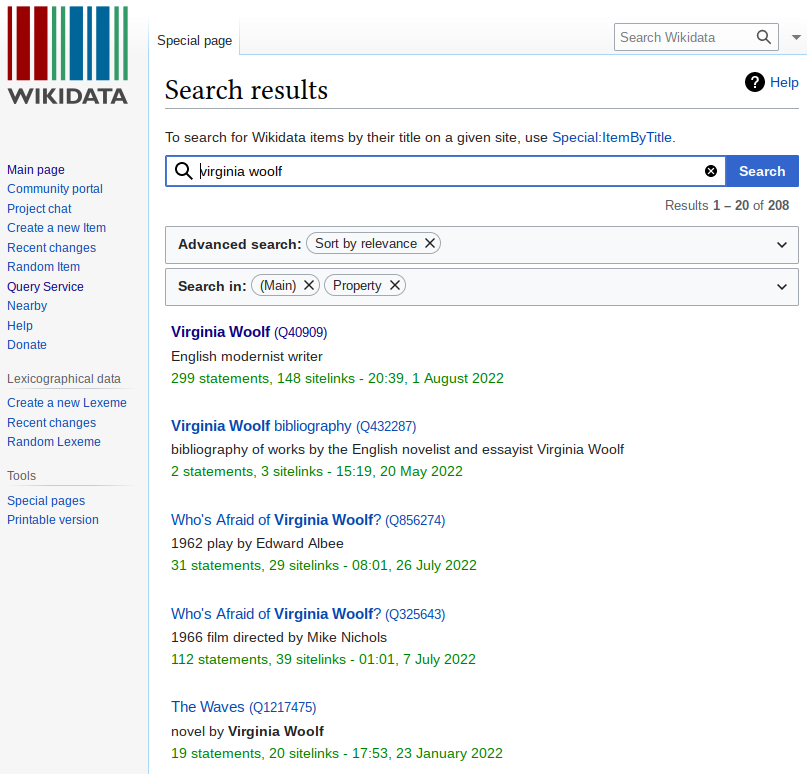
\includegraphics[width=\textwidth]{img/wd_base.png}
		\caption{Résultats retournés par le site traditionnel}
		\label{fig:wd_base}
	\end{subfigure}
	\begin{subfigure}{0.48\textwidth}
		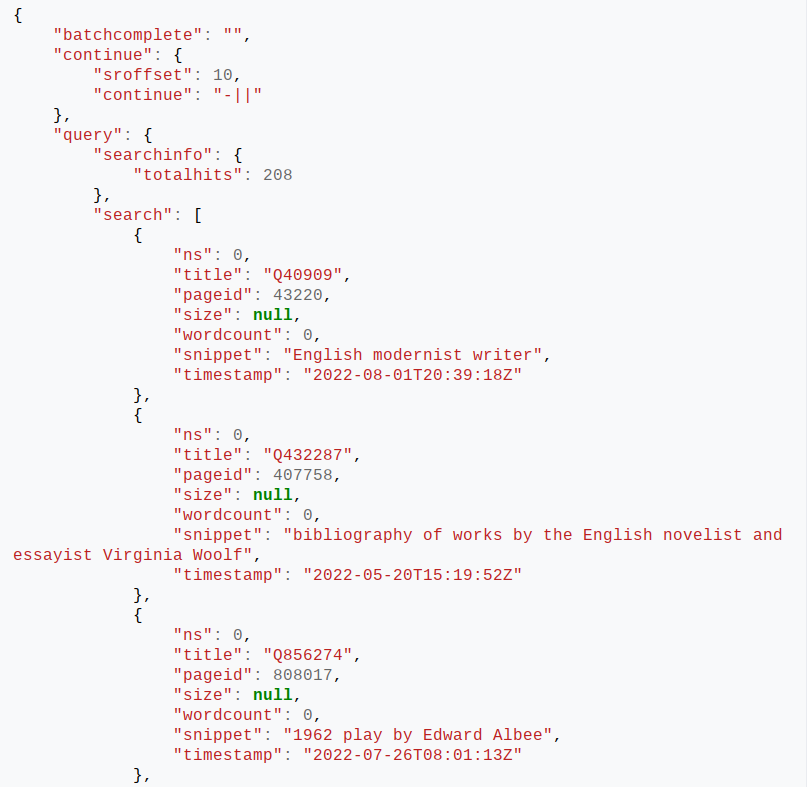
\includegraphics[width=\textwidth]{img/wd_api.png}
		\caption{Résultats retournés par l'\api{}}
		\label{fig:wd_api}
	\end{subfigure}
	\caption{Résultats retournés par \wkd{} pour la recherche \enquote{Virginia Woolf}}
	\label{fig:wd_search}
\end{figure}

Enfin, les données récupérées sont les mêmes, mais dans deux formats très différents (\ref{fig:wd_search}). Dans l'image de gauche (\ref{fig:wd_base}), les résultats sont visibles avec une interface graphique complète, comme sur n'importe quel site Web. À droite cependant (\ref{fig:wd_api}), les résultats sont présentés sous la forme de données structurées au format \json{} (format analogue à un \gls{dictionnaire}). Ce résultat contient à la fois les résultats à proprement parler (en dessous de \enquote{Search}) et des informations descriptives. Par exemple, \texttt{query/searchinfo/totalhits} retourne le nombre de résultats pertinents, soit 208 pages.

Cette brève présentation de la manière de consommer concrètement une \api{} indique également le protocole à suivre pour l'alignement des \tname{} avec des entités \wkd{}: il s'agit de concevoir un algorithme qui, à partir des données extraites du \tname{} et du \ttrait{}, construise des \gls{url} pour lancer des recherches en plein texte sur \wkd{}. Cela revient à associer au paramètre de l'\gls{url} \texttt{srsearch} la chaîne de caractère qui doit être recherchée sur la base de données de \wkd{}. Ensuite, l'algorithme doit transmettre à l'\api{} ces \url{}, interpréter le \json{} renvoyé par \wkd{} et enregistrer ces réponses dans un fichier. Étant donné que l'alignement avec \wkd{} prend plusieurs dizaines d'heures et demande des performances élevées, des \glspl{log} annexes sont créés en cours d'utilisation pour optimiser l'algorithme.


\section{Présentation générale}
L'algorithme d'alignement avec \wkd{} construit des \gls{url} et lance des recherches en plein texte sur l'\api{} \wkd{}. De par son fonctionnement, il multiplie les requêtes. Puisqu'il est impossible de vérifier en cours d'exécution si la réponse retournée par l'\api{} contient un résultat valide, il est nécessaire d'organiser l'algorithme afin de maximiser la probabilité d'obtenir un résultat valide. C'est pourquoi les recherches sont faites en commençant par les celles qui ont la plus grande certitude d'obtenir des résultats valides et en terminant par les plus incertaines. Dès qu'une réponse est obtenue, l'algorithme s'arrête et l'entrée de catalogue suivante est traitée. Comme cela apparaît dans la figure \ref{fig:apialgo}, il a par conséquent un fonctionnement à plusieurs étapes.

La première étape est la même quelles que soient les informations contenues dans le \tname{}: l'ensemble des paramètres\footnote{Dans ce qui suit, le terme \enquote{paramètre} se réfère aux clés du dictionnaire d'informations structurées, et non aux paramètres de l'\api{} présentées ci-dessus (\texttt{srsearch}...).} extraits lors de l'étape précédente sont mis bout à bout afin de lancer une recherche. Cela permet que la recherche soit la plus précise possible, afin de maximiser les possibilités d'obtenir un résultat valide.

Si la réponse de l'\api{} ne contient pas de résultat, alors les données disponibles sont étudiées afin d'adopter le bon comportement. Comme cela a été dit, différents processus ont été utilisés pour extraire des données du \tname{} et du \ttrait{}; il est donc logique de ne pas traiter tous les \glspl{dictionnaire} de données de la même manière.

Si l'entrée concerne une personne noble (c'est-à-dire, si le dictionnaire de données contient un nom de famille noble), alors il y a un possible conflit dans les données extraites: si le nom de famille usuel est recherché en même temps que le nom de famille noble sur \wkd{}, il arrive qu'aucun résultat ne soit retourné. Dans ce cas, une première requête est lancée en supprimant le nom de famille noble; si aucun résultat n'est obtenu, celui-ci est rajouté et c'est le nom de famille usuel qui est enlevé. Pour finir, une autre recherche est lancée sans le prénom. Si à ce stade aucun résultat n'a été obtenu, alors un algorithme de recherches soustractives est lancé; celui-ci est décrit plus bas.

Le deuxième cas de figure concerne la reconstitution des prénoms. Bien que celle-ci augmente la proportion de résultats valides, un prénom mal reconstitué risque de retourner du silence. C'est pourquoi une clé \texttt{rebuilt} a été ajoutée au \gls{dictionnaire} qui contient les données extraites: cette clé permet d'indiquer qu'un nom a été reconstitué. Dans ce cas, une nouvelle recherche est lancée sans le prénom. Si aucun résultat n'est obtenu, alors c'est l'algorithme de recherches soustractives qui s'exécute.

Le troisième cas de figure concerne la présence de plusieurs paramètres de recherche disponibles -- en langage technique, de plusieurs valeurs non-nulles dans le \gls{dictionnaire}. Dans ce cas, c'est directement l'algorithme soustractif qui s'exécute. Celui-ci a été conçu à partir du constat que, d'un côté, les données contiennent inévitablement de bruit; de l'autre, l'extraction de données risque elle aussi d'introduire du bruit. Cette logique soustractive cherche donc à supprimer le bruit qui a pu s'introduire. Afin d'éviter d'être trop \enquote{brut}, l'algorithme procède en séparant les différents types de bruit possibles. D'abord, il arrive souvent qu'un chiffre soit mal reconnu lors de l'océrisation, et il peut donc y avoir des erreurs dans les dates. Deux dates peuvent être extraites (naissance et décès); il y a cependant peu de chances d'erreur sur les deux dates. Par conséquent, une des deux dates est supprimée et la recherche est lancée; si aucun résultat n'est obtenu, c'est l'autre date qui est supprimée. La seconde source de bruit provient des prénoms: comme cela a été dit, au \scl{XIX}, les prénoms étrangers sont régulièrement traduits; il arrive souvent que les prénoms composés ne soient pas dans le même ordre que sur \wkd{}, ou qu'une personne soit nommée par son deuxième prénom -- peut-être parce que les catalogues utilisent des noms d'usage alors que \wkd{} s'en tient aux noms civils. Pour ces raisons, le prénom est retiré de la chaîne de caractères à rechercher avant de faire une requête sur l'\api{}. Bien que les risques liés aux dates et aux prénoms ont été corrigés (autant que possible), il est possible que l'auteur.ice n'ait pas encore été aligné avec une entité \wkd{}. À ce stade, tous les risques spécifiques ont été traités. L'algorithme relance alors des recherches en retirant à chaque fois un paramètre différent, jusqu'à ce qu'un identifiant ait été extrait de \wkd{} ou que toutes les permutations possibles aient été faites.

Cette série de construction d'\gls{url} cherche à minimiser les redondances; cependant, il est possible qu'une même chaîne de caractères puisse être extraite à différentes étapes. C'est pourquoi des \glspl{log} sont créés en cours d'utilisation: ils servent à sauvegarder les chaînes de caractères qui ont déjà été recherchées et les résultats qui leur sont associées. Avant de lancer une requête sur l'\api{}, l'algorithme vérifie donc si la chaîne a déjà été recherchée. Si oui, il récupère le résultat obtenu; sinon, lance la recherche et sauvegarde le résultat retourné par \wkd{}.

L'algorithme de recherche sur \wkd{} est visiblement complexe, puisque son objectif est de minimiser le taux d'erreur possible sur des données variées, ce qui demande d'adopter des comportements différents en fonction des informations disponibles. L'algorithme ayant tendance à retirer de plus en plus de paramètres de recherches en cours d'exécution (les dates, les prénoms...), il est possible que la chaîne recherchée finisse par être très pauvre en informations; cela permet de s'aligner avec une entité, mais celle-ci risque de ne pas correspondre au \tname{} ou d'être très générique. Si l'entité recherchée est \enquote{Napoléon Bonaparte}, mais que suffisamment de paramètres ont été retirés, il est possible que l'algorithme ne recherche que \enquote{Bonaparte}. Le résultat obtenu est alors \href{https://www.wikidata.org/w/index.php?search=bonaparte&search=bonaparte&title=Special%3ASearch&go=Go&ns0=1&ns120=1}{\enquote{Charles Lucien Bonaparte}}. Il est donc utile d'avoir une mesure de la certitude (ou l'incertitude) de la validité d'un résultat, ne serait-ce que pour accélérer le processus de correction des identifiants (ce qui, sur plus de 82000 entrées, n'est pas une mince affaire). Le parti pris a été, tout simplement, d'établir un score de certitude en fonction du nombre de paramètres utilisés pour lancer une recherche. Ce score a été défini de façon expérimentale, en mesurant la proportion de résultats considérés comme certains et ainsi que le taux d'erreur au sein des résultats certains (c'est-à-dire, le nombre de résultats qui ont dépassé le seuil de certitude mais qui sont en fait erronés). Après plusieurs essais différents, le score de certitude \(c_r\) pour un résultat \(r\) a été déterminé. Il suit la formule ci dessous:

\begin{align*}
	\text{Étant donnés:} \\ 
	&c_r \text{ le score de certitude pour un résultat } r \text{;}\\
	&q_r \text{ la chaîne de caractère recherchée pour obtenir le résultat } r \text{;}\\
	&\sum param \text{ la somme des paramètres utilisés dans } q_r \text{;} \\
	&d = 1 \text{ si une date est dans } q_r \text{ ; sinon, } d = 0 \text{;} \\
	&p = 1 \text{ si le prénom utilisé dans } q_r \text{ n'a pas été reconstitué; sinon, } p = 0 \text{;}
\end{align*}
\begin{displaymath}
	c_r = \sum param + d + p
\end{displaymath}

\bigskip
Un résultat est considéré comme étant \enquote{certain} si \(c_{r} >= 4\) ou si des dates sont présentes dans \(q_r\) (les chances qu'un alignement soit fait entre un \tname{} et une entité homonyme ayant les mêmes dates de naissance ou de décès étant très faibles). Sur le jeu de données de test, 32\% des entrées atteignent ce seuil de certitude. 23,6\% de celles-ci comprennent en fait une erreur, soit 8,5\% du jeu de données total (voir le tableau en annexes: \ref{appendix:testfinal}). L'objectif de ce score de certitude n'est pas d'être parfaitement exact, mais d'accélérer la relecture des résultats: en acceptant un taux d'erreur total de 8,5\%, il est possible ne corriger que les entrées pour lesquelles \(c_r < 4\). Seuls les deux tiers du jeu de données restent alors à corriger manuellement.

Cet algorithme cherche à répondre à plusieurs problèmes techniques: il travaille avec des données historiques contenant du bruit et un niveau très inégal d'information. Son fonctionnement vise à maximiser la probabilité d'obtenir un résultat valide, en faisant des requêtes d'abord très spécifiques puis de plus en plus génériques. Cependant, il crée lui-même plusieurs problèmes: son fonctionnement est assez complexe et demande de manipuler plusieurs lourds fichiers en même temps. Un ensemble d'optimisations ont donc été réalisées.

\widepage
\begin{figure}[!p]
	\centering
	\tikz[scale=0.70, transform shape]{
		\node[base] (start) at (-8,8)%
			{Dictionnaire structuré contenant les données à rechercher sur l'\api{}};
		\node[transf] (firsturl) at (0,8)%
			{\textbf{Préparation de la première requête} \\ Premier URL mettant bout à bout tous les paramètres disponibles};
		\node[choice] (type) at (0,1.5)%
			{\textbf{Préparation de la deuxième série de requêtes} \\ Quel type d'entrée est-ce? Quelle données sont disponibles?};
					
		\node[base] (many) at (0,-4)%
			{Plusieurs paramètres de recherche sont disponibles};
		\node[base] (rebuilt) at (8,-4)%
			{Le prénom est reconstitué};
		\node[transf] (rebuilttr) at (8,-9)%
			{Constitution d'un nouvel URL sans le prénom};
		\node[transf] (sub) at (0,-9)%
			{Algorithme soustractif *};
		\node[base] (noble) at (-8,-4)%
			{C'est le nom d'une personne noble};
		\node[transf] (nobletr) at (-8,-9)
			{
				Préparation d'URLS par retrait successif des 
				différentes informations nominatives:
				\begin{itemize}
					\item Prénom
					\item Nom de famille usuel
					\item Nom de famille noble
				\end{itemize}
			};

			
		\node[transf] (launch) at (0,-15)%
			{Lancement de la requête};
		\node[db] (log) at (8,-18)%
			{Fichiers de log};
		\node[transf] (cert) at (0,-20)
			{Évaluation de la certitude du résultat};
		\node[db] (end) at (0,-23)%
			{Enregistrement des résultats};
			
		\node[blank] at (7,-15.3) {Si la première requête ne retourne pas de résultat};
		\node[blank,rotate=-90,text width=3.8cm] at (2.6,-11.8) {Si les deuxièmes séries de requêtes ne retournent pas de résultat};
		\node[blank,text width=4cm] at (4,-16.7) {Vérifier si la requête a déjà été lancée};
		\node[blank,text width=4cm] at (4,-18.6) {\begin{flushright}Enregistrer la requête si elle est lancée\end{flushright}};
		\node[outline, text width=7cm] (note) at (8,7)%
			{
				*: L'algorithme soustractif consiste à:
				\begin{itemize}
					\item si il y a deux dates (naissance et décès), en supprimer une des deux et relancer la requête
					\item si il y a plusieurs paramètres, retirer tous les paramètres un à un et relancer la requête
					\item pour finir, si encore aucun résultat n'a été obtenu, supprimer le prénom et relancer la requête
				\end{itemize}
			};
		\node[blank,text width=3cm,rotate=90] at (-1,-17.25) {Si un identifiant est trouvé, le script s'arrête};
		
			
		\begin{pgfonlayer}{bg}
			\draw[arrow] (start) -- (firsturl);
			\draw[arrow] (firsturl) -- (0,5) -- (-12.5,5) -- (-12.5,-15) -- (launch);
			\draw[arrow] (launch) -- (12.5,-15) -- (12.5,1.5) -- (type);
			\draw[arrow] (type) -- (noble);
			\draw[arrow] (type) -- (rebuilt);
			\draw[arrow] (type) -- (many);
			\draw[arrow] (noble) -- (nobletr);
			\draw[arrow] (many) -- (sub);
			\draw[arrow] (rebuilt) -- (rebuilttr);
			\draw[arrow] (nobletr) -- (-8,-14.5) -- (-2.5,-14.5) -- (launch);
			\draw[arrow] (rebuilttr) -- (8,-14.5) -- (2.5,-14.5) -- (launch);
			\draw[arrow] (sub) -- (launch);
			\draw[arrow] (launch) -- (1.5,-14.5) -- (1.5,-9.75) -- (sub);
			\draw[arrow] (launch) -- (cert);
			\draw[arrow] (cert) -- (end);
			\draw[arrow] (launch) -- (1.5,-15.5) -- (1.5,-17.25) -- (5.5,-17.25) -- (log);
			\draw[arrow] (launch) -- (1.5,-15.5) -- (1.5,-18.25) -- (5.5,-18.25) -- (log);
		\end{pgfonlayer}	
		
	}
	\caption{Algorithme lançant des recherches en plein texte sur \wkd{}}
	\label{fig:apialgo}
\end{figure}
\restoregeometry

\section{Gérer la montée en charge: optimisation et réduction du temps d'exécution}
\sectionmark{Gérer la montée en charge}
L'intégralité de l'algorithme (contenant extraction d'informations et interaction avec une \api{}) a cessé de fonctionner sur mon ordinateur alors qu'à peine 5\% des 820000 entrées avaient été traitées. Ce problème technique soulève des difficultés adjacentes à la recherche en humanités numériques: dans ce contexte, des ordintateurs très performants ne sont pas toujours disponibles, et les machines utilisées sont souvent des ordinateurs de bureau traditionnels. De telles situations, la recherche peut parfois faire face à des limitations matérielles. De telles limites sont -- bien sûr -- un problème; en obligeant chercheur.euse.s à intégrer des contraintes matérielles dans leurs algorithmes, cette difficulté peut aider à réaliser des programmes plus efficaces, moins gourmands en ressources et en énergie, et donc aider à faire de la recherche plus durable. De telles considérations écologiques sont partagées par toute une communauté de chercheur.euse.s issu.e.s des humanités et défendant des approches \enquote{low-tech}\footnote{
	Le \textit{Minimal computing} (\enquote{Informatique minimale} en français) est un groupe de réflexion créé au sein de \textit{GO::DH -- Global Outlook Digital Humanities}. Il s'intéresse aux manières de rendre l'informatique minimale, dans différents sens du terme: à la fois plus accessible, mais également plus écologique. Plus généralement, le courant du \textit{minimal computing} développe une approche réflexive sur les façon de faire de la recherche durable et libre (au sens de l'\gls{open source}); ce groupe s'intéresse également au développement des humanités numériques dans un contexte non-occidental\cite{sayers_minimal_2016}.
}; ces considérations écologiques sortent du champ des humanités et se retrouvent dans des travaux provenant de l'informatique \enquote{traditionnelle} et de l'apprentissage machine\footcite{strubell_energy_2019}. L'optimisation de programmes informatique n'est pas seulement une question écologique: c'est également une manière d'écrire de meilleurs programmes, plus performants et efficaces.

Dans sa première version, le script d'alignement avec \wkd{} avait un fonctionnement apparemment plus \enquote{simple}, puisqu'il ne prenait pas du tout en compte les questions d'optimisation: pour chaque entrée de catalogue, des informations étaient extraites et les recherches faites sur \wkd{}. Ce fonctionnement avait deux défauts. D'abord, il demandait que tout le script soit exécuté en une fois -- si il y a une erreur imprévue, il est nécessaire de recommencer à nouveau. Ensuite, une interaction avec \wkd{} était nécessaire pour chaque entrée, peu importe si le nom contenu dans le \tname{} avait déjà été recherché auparant (alors qu'une même personne est souvent l'auteur.ice de plusieurs manuscrits recensés dans les catalogues); l'interaction avec \wkd{} prenant plusieurs secondes, cela peut grandement ralentir le processus d'alignement avec \wkd{}. C'est à partir de ces deux problèmes que le processus d'optimisation a commencé.

Le premier problème -- l'impossibilité de vérifier quelles entrées de catalogue ont déjà été traitées -- a d'abord été corrigé en consultant, à chaque fois qu'un nouvel identifiant était recherché, le fichier de sortie. Celui-ci est un tableur qui contient l'identifiant des entrées, le \tname{}, le \ttrait{}, l'identifiant récupéré sur \wkd{} et un extrait de la description associée à cet identifiant. Si cette solution permet de ne pas recommencer à zéro à chaque fois que le script est lancé, elle demande de charger en mémoire un très large fichier \texttt{csv} (12,7 mégaoctets). Cette vérification particulièrement gourmande a été remplacée par la création d'un \gls{log} annexe en cours d'exécution. Celui-ci contient uniquement les identifiants des différentes entrées de catalogue et mesure seulement 1,3 mégaoctets. À chaque fois qu'une nouvelle entrée est traitée, ce fichier est ouvert, et le script vérifie que le nouvel identifiant ne s'y trouve pas. Si l'identifiant ne s'y trouve pas, alors le \tname{} et le \ttrait{} de cette entrée sont traités et alignés avec un identifiant \wkd{}. À la fin de ce processus, l'identifiant \tei{} de l'entrée est ajouté au \gls{log}. Cette simple modification permet donc de vérifier si une entrée de catalogue a déjà été traitée à l'aide d'un fichier dix fois moins lourd que dans la tentative précédente.

Ce processus permet de vérifier quelles entrées ont déjà été traitées, mais il ne permet pas de savoir si une personne se retrouve d'une entrée sur l'autre. Si une telle récurrence est identifiée, il serait possible de récupérer les résultats déjà disponibles, plutôt que de réaliser à nouveau l'alignement avec \wkd{}. Non seulement cela pourrait rendre le script plus rapide -- le lancement des requêtes pour une entrée prenant environ 2 à 5 secondes --, mais en plus, cela éviterait de surcharger l'\api{} de requêtes, ce qui, dans un cas extrême, peut faire saturer une application en ligne et perturber son fonctionnement. La difficulté consiste alors à désambiguïser les informations présentes dans le \tname{} (c'est-à-dire, à repérer toutes les occurrences d'une même personne dans les \tname{}). Cette désambiguïsation est compliquée (l'un des intérêts de la reconnaissance d'entités nommées est justement d'identifier les multiples occurrences d'une même personne). Plutôt que de trouver un moyen de désambiguïser réellement les entrées, une solution plus simple a été mise en place: chaque chaîne de caractère recherchée est enregistrée dans un \gls{log}, avec l'identifiant \wkd{} récupéré par recherche. L'intégralité du processus d'extraction d'information des \tname{} et \ttrait{} est donc menée sur toutes les entrées; toutes les chaînes de caractères à rechercher sont également construites; cependant, une recherche n'est faite sur l'\api{} que si elle n'a jamais été faite auparant. Du fait de la taille du jeu de données, un problème apparaît cependant: plusieurs chaînes de caractères étant construites pour chaque entrée de catalogue, l'utilisation d'un seul \gls{log} pour contenir toutes ces recherches amènerait à la création d'un immense fichier (plusieurs centaines de milliers de lignes). Il serait alors nécessaire de le parcourir intégralement à chaque fois qu'une requête est lancée; le script optimisé risquerait alors d'être moins efficace qu'avant son optimisation. Le choix a donc été fait de créer automatiquement et d'utiliser plusieurs \glspl{log}: les chaînes de caractères y sont enregistrées en fonction du premier caractère qu'elles contiennent, avec un \gls{log} par lettre. Ainsi, avant de lancer une recherche, le fichier à parcourir est bien plus court (2060 entrées pour la lettre \enquote{e}).

Avec toutes ces optimisations, le script a pu fonctionner en utilisant au maximum 3 gigaoctets, soit l'équivalent de naviguer sur internet en ayant un logiciel de traitement de texte ouvert (sur ma machine). Cependant, l'utilisation \glspl{log} faite ici -- qui a elle même été optimisée -- demande de faire un arbitrage. En n'enregistrant pas de données et en lançant des requêtes à chaque fois, c'est la charge processeur qui augmente, ainsi que la consommation de courant due à internet. En enregistrant les requêtes déjà lancées, ces charges là sont diminuées, mais l'utilisation de mémoire vive augmente (il faut charger en mémoire et lire de larges fichiers). De ces deux deux différentes approches (augmenter la charge processeur ou augmenter la mémoire vive) il est nécessaire de déterminer laquelle est la plus efficace. C'est un des objectifs des tests menés sur l'algorithme d'alignement avec des identifiants \wkd{}, comme nous allons le voir maintenant.

\section{Évaluer la résolution d'entités : performance, qualité des données extraites de \wkd{} et comparaison avec d'autres projets}
\sectionmark{Évaluer la résolution d'entités}
Le processus d'alignement avec des entités \wkd{} n'est pas parfait, et implique nécessairement un taux d'erreur. Au vu de la taille du corpus, la correction des résultats est un processus particulièrement chronophage. Pour pouvoir utiliser les données produites avant cette correction, il est nécessaire de trouver une manière d'évaluer la qualité des résultats. Des tests ont été réalisés pour faire cette évaluation. Ils ont également été utilisés durant tout le développement de ce processus, afin de comparer les différents algorithmes d'extraction et de requêtes entre eux. Les tests ont également permis de mesurer l'impact de chaque paramètre de recherche dans l'obtention d'un résultat valide. Enfin, l'évaluation des algorithmes permet de comparer sa version optimisée et non-optimisée.

Comme cela a déjà été dit, les tests ont été lancés sur un jeu de données représentatif contenant 200 \tname{} et \ttrait{}, choisis dans différents catalogues; ce jeu de test représentant également les différents types de noms possibles (de personnes nobles, de lieux...); enfin, la proportion de \ttrait{} dans le jeu de données complet et dans celui de test est la même. Deux catégories de tests ont été réalisés. Le premier, décrit plus haut, concerne l'impact de chaque paramètre dans l'obtention d'une entité correcte sur \wkd{} (\ref{appendix:testisolate}). Le second sert à mieux identifier les performances de l'algorithme final (\ref{appendix:testfinal}). 

Ce dernier test réalise l'intégralité du processus d'extraction d'informations et d'alignement avec \wkd{} sur l'ensemble du jeu de test. Ce processus est réalisé trois fois sans utiliser des \glspl{log} et trois fois en les utilisant (c'est-à-dire, en inscrivant les recherches déjà faites dans un fichier et en vérifiant avant chaque recherche si une chaîne de caractère a déjà été recherchée). Faire plusieurs fois de suite le même processus permet de les variations de performance induites par l'utilisation de \glspl{log}. La performance d'un script, en terme d'utilisation des processeurs et de la mémoire vive, est assez difficile à quantifier; elle peut également varier d'une machine à une autre; enfin, il n'est pas possible de mesurer la charge supplémentaire infligée à un serveur distant lors de l'utilisation répétée de sources de données en ligne. Le seul critère retenu a donc été le temps d'exécution. Le script étant lancé trois fois en utilisant des \glspl{log} et trois fois sans, les deux temps d'exécution \(\bar{t}\) correspondent au temps moyen nécessaire à traiter les 200 entrées du jeu de test. Soit \(t_i\) le temps pris pour traiter une fois le jeu de test, la moyenne \(\bar{t}\) correspond à:

\begin{displaymath}
	\bar{t} = \frac{1}{3}\sum_{i=1}^{3}t_i
\end{displaymath}

La difficulté pour mesurer les temps d'exécution \(t_i\) en utilisant des \glspl{log} est que, en dehors des tests, ces fichiers sont de plus en plus volumineux; le temps utilisé pour les parcourir augmente en conséquence. Pour que ces \(t_i\) soient représentatifs, de faux \glspl{log} sont créés avant le lancement des tests: ceux-ci comprennent des fausses données qui correspondent environ aux résultats obtenus pour 30000 recherches lancées sur l'\api{} (soit un peu moins que les 82000 entrées du jeu complet, en prenant en compte que certaines recherches ne retournent pas de résultat, ce qui allège d'autant le fichier à parcourir). Le temps d'exécution \(\bar{t}\) en utilisant des \glspl{log} est de 88,3 secondes; sans ces fichiers, \(\bar{t}\) est de 92,5 secondes. Si la différence entre les deux résultats n'est pas immense, l'utilisation de \glspl{log} permet également la charge processeur et l'interaction avec \wkd{}, ce permet d'autres améliorations au delà du seul temps de performance.

À part cette seule évaluation de performance, les tests sur l'algorithme final (\ref{appendix:testfinal}) servent à mesurer la qualité des résultats obtenus. La mesure de performance pour un processus d'alignement est le \gls{score F1}, qui prend à la fois en compte la précision (le nombre de vrais positifs obtenus parmi tous les résultats obtenus) et le rappel (le nombre de vrais positifs obtenus parmi tous les vrais positifs). Celui-ci est de 67,4\%, ce qui marque une nette amélioration (près de 20 points) de l'utilisation seule du prénom et du nom de famille usuel extrait du \tname{}. 

Ce score est également intéressant en comparaison avec d'autres projets de \gls{nel}, sous-domaine du traitement automatisé du langage qui vise à associer une entité avec une base de connaissances externes. Aicha Soudani et al. ont, en 2018, présenté les résultats d'un projet de \gls{nel} de lieux sur un corpus relativement proche du notre: des textes littéraires du \scl{XIX} encodés en \xmltei{}. \footcite{soudani_adaptation_2018}. Les méthodes utilisées par ce projet diffèrent largement de celles présentées ici: les auteur.ice.s s'appuient fortement sur l'apprentissage machine, en identifiant d'abord des entités dans le texte à l'aide de \texttt{SEM} avant de lier les entités à différentes bases de connaissance en utilisant \texttt{REDEN}. Leur projet présente donc une complexité supplémentaire, puisqu'il demande de repérer les entités, ce qui n'est pas le cas ici (elles se trouvent toutes dans des balises \tname{}). Cependant, c'est cette deuxième étape qui nous intéresse; les entités ont déjà été identifiées, ce qui nivelle cette différence entre les projets. Trois bases de données en ligne ont été utilisées: \textit{DBPedia}, \textit{DataBnF} et \wkd{}. En comparaison avec ce projet, il est intéressant de remarquer que le processus d'alignement avec \wkd{} développé par \mssktb{} obtient un \gls{score F1} très satisfaisant (67,4\%). Celui-ci dépasse les scores obtenus par Soudani et al. dans leur alignement avec \wkd{} (61,1\%) et \textit{DBPedia} (53,6\%)\ (voir le détail des résultats en annexe: \ref{appendix:soudani}). Les résultats comparativement faibles de Soudani et al. s'expliquent en partie par le fait que \texttt{REDEN} recherche des candidats pour le liage d'entités en établissant une correspondance parfaite des caractères (\textit{exact string match})\footcite[p. 4]{soudani_adaptation_2018}\footnote{Il est également à remarquer que Soudani et al. disposent d'un score d'\enquote{exactitude totale du liage} (\textit{Overall linking accuracy}) qui est nettement plus élevé (entre 70 et 85\%); la méthode de calcul de ce score, qui mesure la performance de l'ensemble du processus de \gls{nel}, n'est cependant pas décrite dans l'article. Il est donc impossible d'y comparer les résultats de \mssktb{}.}. Les scores comparativement positifs du projet \mssktb{} sont peut être également rendus possibles par la quantités d'informations disponibles sur chaque personne dans le corpus, récupérée grâce à un travail d'extraction des données sur l'ensemble du \ttrait{} et du \tname{}.

\section{En conclusion: retour sur l'extraction d'informations des catalogues et sur l'algorithme d'alignement avec \wkd{}}
\sectionmark{En conclusion}
L'algorithme liant les noms d'auteur.ice dans les catalogues avec des entités \wkd{} propose une réponse à plusieurs difficultés techniques propres à la reconnaissance d'entités par la détection de motifs sur un corpus de données varié. Parmi toutes ces difficultés possibles, les trois les plus importantes sont le bruit dans les données d'origine, le bruit produit par l'extraction de données et enfin la difficulté à réaliser un alignement entre des documents historiques et des bases de données contemporaines. La solution proposée s'appuie sur un fonctionnement modulaire, qui s'adapte aux données produites et prend en compte la possibilité que du bruit se soit introduit à une étape ou à une autre. De différence de résultats obtenue avec Soudani et al., il faut retenir que la technique utilisée n'est pas toujours garante de la qualité des résultats obtenus. Plutôt que de chercher à établir des correspondances exactes, l'approche décrite dans ce mémoire, basée sur une détection de motifs \textit{low-tech} a permis de développer une méthode très précisément adaptée à la fois au corpus et à \wkd{}. Ce qui est potentiellement perdu par la détection de motifs est donc corrigé par l'algorithme menant des requêtes sur \wkd{}. 

L'alignement avec des entités \wkd{} est la meilleure manière de corriger le bruit dans les données du projet: en liant les différents \tname{} à des identifiants \wkd{}, il devient possible d'extraire des données structurées d'une source externe, pour construire une base de connaissance plus fiable: même si un corpus semi-structuré facilite le travail d'extraction d'informations, l'accès aux informations reste relativement complexe; il existe de plus des biais dans les informations contenue par le corpus (ce qui est mis en avant dans les \ttrait{} est avant tout ce qui est susceptible d'intéresser le public de l'époque). En se servant de ce liage d'entités pour constituer une base de données, il est possible de chercher à corriger ce biais dans les données, tout en rassemblant assez d'informations pour pouvoir faire une analyse des facteurs déterminant le prix d'un manuscrit sur le marché du  \scl{XIX}. C'est la manière dont est constitué le jeu de données issu de \wkd{} qui est expliqué ci-dessous.

\chapter{Après l'alignement, l'enrichissement: utiliser \sparql{} pour produire des données structurées}
\chaptermark{Après l'alignement, l'enrichissement}
Le liage des noms contenus dans le \tname{} avec \wkd{} n'est qu'une étape, et non la fin en soit du processus -- bien que ce soit la partie la plus difficile. Les identifiants ainsi récupérés servent de \enquote{porte d'entrée} aux données disponibles sur la base de connaissance: une fois que ces identifiants sont connus, il est possible de récupérer automatiquement via \sparql{} des données sur les auteur.ice.s et autres entités présentes dans les catalogues. Obtenir ces informations permet avant tout de mieux situer l'auteur.ice d'un manuscrit, afin mieux le statut d'une personne et de comprendre quelles informations biographiques influencent le prix d'un manuscrit. Mais le liage d'entités nommées peut avoir d'autres fins et permettre d'enrichir le corpus de catalogues de plusieurs manières, comme nous le verrons.

\section{Comprendre les particularités des modèles sémantiques de données}
\sectionmark{Comprendre les particularités...}
Un bref retour sur la manière dont s'organisent les données contenues dans \wkd{} permet de mieux comprendre le problème que peut poser la diversité du corpus pour la constitution d'une base de connaissances propre au projet. \wkd{}, comme de nombreuses autres bases en lignes (\textit{DataBnF, DBPedia...}), permet d'accéder à des informations stockées dans une \gls{graph}. Ce type de base de données a un fonctionnement très particulier qui influence la constitution d'une base de connaissance à partir des identifiants \wkd{} récupérés à l'étape précédente. Dans une \gls{graph}, les données sont encodées en \xml{}-\rdf{}. Ce format -- dit sémantique -- contient des données liées sous forme de \enquote{triplets} sujet--prédicat--objet, où:

\begin{itemize}
	\item le sujet est la ressource principale.
	\item le prédicat est une propriété du sujet, qui caractérise une relation avec une autre ressource, l'objet.
	\item l'objet est une ressource secondaire: c'est la valeur d'un prédicat.
\end{itemize}

Le principe des triplets \rdf{} est mieux exprimé sous forme graphique (\ref{fig:triplet}):

\begin{figure}[!h]
	\centering
	\tikz{
		\node%
		[base] %
		(S) at (0,0) %
		{\textbf{Sujet} \small \\ La ressource principale \\ \textit{Natalia Gontcharova}};
		\node%
		[transf] %
		(P) at (5, 0) %
		{\textbf{Prédicat} \small \\ La relation à l'objet \\ \textit{a peint}};
		\node%
		[base] %
		(O) at (10, 0) %
		{\textbf{Objet} \small \\ Une ressource secondaire \\ \enquote{\textit{Les porteuses}}};
		
		\draw[arrow] (S) -- (P);
		\draw[arrow] (P) -- (O);
	}
	\caption{Exemple de relation sujet -- prédicat -- object}
	\label{fig:triplet}
\end{figure}

Trois particularités supplémentaires définissent les formats sémantiques:
\begin{itemize}
	\item Toutes les \enquote{ressources} peuvent être tour à tour sujet ou objet. L'exemple du dessus, par exemple, aurait pu être réécrit sous la forme: \enquote{Les porteuses} a été peint par Natalia Gontcharova. Dans ce cas, Natalia Gontcharova est l'objet et \textit{Les porteuses} est le sujet. Par conséquent, une base de données \rdf{} est une \gls{graph}; elle peut être représentée sous la forme d'un réseau de ressources qui entretiennent des relations bilatérales entre elles. Il n'y a pas de hiérarchie entre les informations, contrairement à une base de données \xml{} classique.
	\item L'ensemble des ressources et des prédicats d'une \gls{graph} sont définis et disposent d'un identifiant unique (certains de ces identifiants ont été récupérés grâce au liage d'entités nommées).
	\item Si le langage \sparql{} offre une syntaxe commune, chaque base de connaissance peut utiliser des vocabulaires particuliers qui sont organisés en \enquote{ontologies}. Une ontologie correspond à la définition d'un ensemble de catégories, de propriétés et de relations qui unissent des données et des concepts; cet ensemble est complété par une modélisation (souvent sous forme graphique), qui indique la relation entre les différents termes de l'ontologie\footcite{noauthor_ontology_2022}. Ceux-ci sont souvent liés de façon hiérarchique (plusieurs termes spécifiques pouvant être dérivés d'un terme générique). Au sein d'une ontologie, chaque terme a lui-même un identifiant unique, ce qui garantit une implémentation uniforme pour l'ontologie. Une même base de connaissance peut utiliser plusieurs ontologies. Celles-ci sont définies à l'aide d'espaces de noms\footcite{noauthor_namespace_2022}, c'est-à-dire par des identifiants qui permettent de différencier les ontologies. Les prédicats, plus particulièrement, sont définis selon une ontologie particulière.
\end{itemize}

\sparql{} a l'avantage de permettre de récupérer des données propres sur des bases en ligne et offre une syntaxe unique partout où il est implémenté. Cependant, le troisième point complexifie son utilisation, ainsi que la définition des données à récupérer: les prédicats sont décrits avec une grande précision et selon des vocabulaires spécifiques; par conséquent, une information analogue peut être représentée par différents prédicats selon le type de donnée qui est requêtée (une personne, une sculpture...). Dans l'ontologie \wkd{}, la création d'un texte et la création d'une peinture ne correspondent pas au même prédicat. Pour que les données soient utilisables, il faut être très spécifique quant aux informations recherchées. 

\section{Quelles données rechercher via \sparql?}
La question des données qui doivent être récupérées, et donc de la base de connaissance à constituer pour le projet \mssktb{} n'est pas anodine. D'abord, l'utilisation de sources externes peut être utiliser pour corriger des biais dans les données originelles (où ce sont les auteur.ice, éditeurs et éditrices de catalogues qui décident des informations à intégrer). Ensuite, si l'objectif premier est de récupérer des données pour mener une étude économétrique, le liage avec \wkd{} peut également permettre d'autres enrichissements et fonctionnalités. Enfin, cette étape représente une difficulté technique: le corpus de catalogues et les entités récupérées sont très diverses, tandis que \sparql{} utilise au contraire des vocabulaires très spécifiques. Il faut donc construire des requêtes très étendues, afin d'obtenir des résultats pour tous les types de données. Les 18899 entités avec lesquelles les entrées de manuscrits ont été alignées peuvent se classer en de nombreuses catégories. Sur \wkd{}, une entité est une \enquote{instance} d'une classe plus large. C'est en fonction de ces classes qu'il faut construire les requêtes: les propriétés recherchées pour chaque entité peuvent être spécifiques à une classe, mais pas à l'entité elle-même. En suivant la classification de \wkd{}, les entités présentes dans le corpus appartiennent aux catégories suivantes:

\begin{itemize}
	\item personnes humaines; cette catégorie est la plus fréquente (12090 occurrences)
	\item noms de familles (3180 entités)
	\item communes françaises (586 occurrences)
	\item peintures et sculptures (respectivement 520 et 236 entités)
\end{itemize}

Cette variété -- présentée sous forme graphique en annexes (\ref{appendix:wikidata_instances}) -- peut s'expliquer en partie par le taux d'erreur dans l'alignement avec \wkd{}: il est par exemple probable que les peintures et sculptures soient sur-représentées parmi les entités \wkd{} liées aux catalogues. Cependant, toutes ces \enquote{erreurs} ne correspondent pas forcément à des résultats qui ne sont pas pertinents. Par exemple, l'algorithme peut aligner un.e écrivain.e avec un de ses ouvrages, ou une personne avec son portrait. Des résultats erronés peuvent toujours garder une forme de pertinence. Il est d'autant plus important de construire des requêtes \sparql{} qui se concentrent pas uniquement sur des personnes. Cependant, il n'est pas possible de s'adapter à l'intégralité de la diversité du corpus. Le choix a donc été fait de se concentrer sur les catégories les plus pertinentes: les personnes, les familles, et les œuvres artistiques et littéraires. Non seulement ces catégories contiennent la grande majorité du corpus (16026 entités, soit 84,79\%), mais ces catégories sont les plus à même de contenir des entités pertinentes. Il a été choisi de ne pas faire de requête spécifique sur les lieux, puisque \wkd{} présente peu d'informations pour les entités de la catégorie \enquote{communes françaises}.

Un nombre assez conséquent de données ont donc été requêtées avec \sparql{}, du fait des spécificités des bases de données en graphes, de la variété des entités \wkd{} auxquelles les manuscrits sont liées, et enfin du fait de la variété du corpus lui même. Ces informations récupérées correspondent aux différentes catégories de \wkd{}.
\begin{itemize}
	\item Pour les personnes et les familles, les informations suivantes sont récupérées sur \wkd{}:
	\begin{itemize}
		\item Le genre de la personne;
		\item Sa nationalité, afin de voir si l'origine d'une personne influence le prix d'un manuscrit;
		\item Les langues parlées par une personne; là encore, l'objectif est d'étudier l'impact de l'origine d'un.e auteur.ice sur un prix.
		\item Les date de naissance et de décès, afin de placer un manuscrit dans une époque et de voir comment son ancienneté ou sa contemporanéité en influencent le prix.
		\item Le lieu où une personne est née, où elle a vécu et où elle est morte, pour des raisons analogues.
		\item La manière dont la personne est morte. Si cette information peut sembler anecdotique à un public contemporain, les catalogues de ventes sont marqués par un goût du sensationnel, et la manière dont une personne est morte est souvent mentionnée, notamment en cas d'exécutions.
		\item La religion d'une personne: il peut être intéressant d'étudier si, et comment, ce critère influence l'évolution d'un prix.
		\item Les titres de noblesse d'une personne.
		\item L'éducation qu'a reçu une personne, afin de mieux situer ses occupations et d'analyser l'impact du niveau et du type d'éducation sur le prix.
		\item L'occupation d'une personne, et les fonctions précises qu'elle a occupées: là encore, il est intéressant de situer l'impact de la carrière sur le prix et de voir quelles occupations sont corrélées avec des prix élevés sur le marché des manuscrits.
		\item Les prix et distinctions reçus par une personne. À l'aide de ce critère, il est alors possible de chercher à répondre à cette question: la célébrité d'une personne de son vivant impacte-elle le prix de se manuscrits?
		\item Les organisations et institutions dont la personne est membre (Académie française, Franc-maçonnerie...)
		\item Le nombre d'œuvres écrites ou réalisées par une personne. Là encore, c'est une tentative de mesurer l'impact ou la célébrité d'une personne: les manuscrits de quelqu'un ayant beaucoup écrit sont ils plus chers que les manuscrits d'une personne ayant peu écrit ?
		\item Le nombre de conflits auxquels une personne a participé. Ce critère de recherche permet de quantifier l'importance d'un personnage militaire.
		\item Des images, telles que le portrait et la signature.
	\end{itemize}
	\item Pour les créations littéraires, ce sont des informations bibliographiques qui sont avant tout récupérées; pour les autres œuvres d'art, des informations analogues sur le contexte de création sont retenues.
	\begin{itemize}
		\item Le titre de l'œuvre.
		\item Son auteur.ice, pour étudier si certain.e.s auteur.ice.s sont susceptibles d'influencer le prix d'un manuscrit.
		\item La date de création de l'œuvre, afin de savoir si l'époque d'origine influence le prix. Pour les livres, la date publication est également récupérée.
		\item La requête récupère aussi la maison d'édition d'un livre.
		\item Les dimensions et matériaux d'une œuvre d'art sont également d'intérêt.
		\item Enfin, le genre et le mouvement dans lequel s'inscrivent une œuvre sont d'intérêt: ces informations pourraient permettre de voir si une hiérarchie des du goût influence le prix d'un manuscrit.
	\end{itemize}
	\item Pour finir, afin de pouvoir éventuellement enrichir nos données avec d'autres sources externes à \wkd{}, des identifiants uniques ont été récupérés afin de donner accès à d'autres bases de données en ligne: les identifiants VIAF (Fichier d'autorité international virtuel), ISNI (International Standard Name Identifier), de la Bibliothèque nationale de France, de la Bibliothèque du Congrès américain, ainsi que les identifiants IDRef. Certaines insitutions, comme la BnF, rendent leurs données accessibles via \sparql{}; la récupération de ces identifiants faciliterait grandement les enrichissements ultérieurs depuis d'autres sources de données.
\end{itemize}

Comme on l'a dit, l'objectif principal de l'alignement avec \wkd{} est de produire des données pour calculer des régressions linéaires, ce qui permettrait d'étudier les déterminants du prix d'un manuscrit sur le marché du \scl{XIX}. Cette récupération d'informations en masse ouvre d'autres possibilités. Entre autres, de nombreuses données géographiques ont sont récupérées (lieu de naissance, de décès, d'inhumation et de résidence). Il est ensuite possible  de récupérer les coordonnées de ces lieux, afin de construire une cartographie des auteur.ice.s dont les manuscrits circulent sur le marché du \scl{XIX} parisien. C'est d'ailleurs souvent à des visées cartographiques et de géoréférencement que sont menées des campagnes de reconnaissance d'entités nommées; dans les dernières années en France, de nombreuses études ont été menées pour développer des cartographies à partir de textes littéraires français encodés en \tei{} (Soudani et al.\footcite[p.4-5]{soudani_adaptation_2018}, \footcite[p. 63-66]{frontini_annotation_2016}). En développant une approche cartographique, le projet \mssktb{} pourrait apporter de nouvelles possibilités pour de telles études: le corpus de catalogues étant une source secondaire sur l'histoire littéraire française, une approche géographique permettrait d'étudier les origines géographiques des auteur.ice.s, plutôt que d'analyser les lieux représentés dans leurs œuvres. Cette possibilité n'est pas anodine, puisqu'elle permettrait de mettre en relation la \enquote{parisianité} avec la construction du canon littéraire à Paris. Il serait également possible d'étudier la circulation des productions culturelles, et leur rayon d'influence. En croisant les données géoréférencées avec des informations chronologiques (dates de naissance et de mort...), ces questions peuvent également être étudiées de façon historique: comment l'influence de l'origine géographique sur la réception d'une œuvre évolue au fil des siècles? Répondre à ces questions n'a pas été possible dans le cadre de mon stage; cependant, grâce à l'enrichissement de données via \sparql{}, il de telles études deviennent possibles, et les données pour mener ces analyses sont au moins en partie déjà disponibles. Produire des informations normalisées et exploitables pour la recherche implique donc de produire des données qui puissent être réutilisées avec d'autres problématiques de recherches.

\section{Présentation générale}
L'algorithme de récupération des informations sur \wkd{} est considérablement plus simple que ce qui a été présenté lors de l'extraction d'informations des catalogues et de l'alignement avec des entités \wkd{}: lors de ces étapes, les principales difficultés résultaient du bruit dans les données et de la nature \enquote{semi-structurée} des entrées de catalogues, qui demandait de s'adapter à de nombreux cas de figure. Une fois que des identifiants \wkd{} ont été extraits, le processus est bien plus simple -- comme cela apparaît dans la figure \ref{fig:sparqlalgo}. Un identifiant étant unique et servant de clé d'entrée à une \gls{graph} très structurée, un comportement uniforme peut être adopté pour récupérer des données issues de \wkd{}. Il ne s'agit plus que, pour chaque identifiant \wkd{} récupéré, de lancer des requêtes \sparql{} et d'en stocker le résultat dans un fichier. Le comportement de l'algorithme est donc toujours le même.

L'algorithme commence par vérifier si un identifiant a déjà été traité dans un \gls{log}; l'utilisation de ces fichiers évite d'avoir à recommencer la récupération d'informations de \wkd{} à chaque interruption du script, ce qui est essentiel puisque cette étape dure plus de dix heures. Si l'identifiant n'a pas été traité, alors plusieurs requêtes \sparql{} sont lancées sur \wkd{}. Les résultats sont retournés en \json{} ou \xml dans des formats définis dans une spécification du W3C\footcite{beckett_sparql_2013}. Ceux-ci ont un but descriptif (ils décrivent la requête et les données retournées); les documents \sparql{} sont donc très complets et peu malléables; c'est pourquoi ils sont transformés en une base de connaissance au format \json{}. Celle-ci, comme nous le verrons, ne contient que les données obtenues dans un format plus malléable.

Les requêtes \sparql{} sont faites sur un serveur distant via le protocole \gls{http} et demandent parfois au serveur de traiter de très grandes quantités de données. Des erreurs peuvent donc avoir lieu. Pour permettre au script de fonctionner malgré ces erreurs, un système de gestion des erreurs a donc été mis en place. Par défaut, il est demandé au serveur de \wkd{} de fournir les résultats de la requête en \json{}, format très léger et malléable. Deux erreurs peuvent alors arriver: soit le \json{} retourné par le serveur est mal formé (et ne peut donc être traité), soit la requête met plus excède la durée maximale autorisée (qui est d'une minute). Dans ce cas, la requête est lancée une seconde fois au serveur, mais cette fois-ci le format de réponse demandé est le \xml{}; cela permet d'éviter que le document soit mal formé; il est également possible que la requête s'exécute dans le temps imparti la seconde fois. Si une erreur a encore lieu à la seconde requête, alors une entrée vide est associée à l'identifiant \wkd{} dans la base de connaissance, pour signifier qu'aucune réponse n'a pue être obtenue.

\widepage
\begin{figure}[ph!]
	\centering
	\tikz{
		\node[base] (start) at (0,5)
			{Identifiant \wkd{}};
		\node[transf] (1sparql) at (0,2)
			{Première requête \sparql{} avec réponse au format \json{}};
		\node[choice] (1return) at (0,-2)
			{La réponse est-elle valide?};
		\node[transf] (2sparql) at (-5,-5)
			{Seconde requête \sparql{} avec réponse au format \xml{}};
		\node[choice] (2return) at (-5,-9)
			{La réponse est-elle valide?};
		\node[transf] (2empty) at (-9,-13)
			{Construction d'une entrée vide dans la base de connaissance};
		\node[db] (end) at (0,-16)
			{Base de connaissances issues de \wkd{}};	
		\node[db] (log) at (5,-9)
			{\Gls{log} contenant une liste d'identifiants déjà traités};
		
		\node[blank,rotate=-90,text width=10cm] at (5,-1)
			{	
				Vérification de si l'identifiant a déja été traité 
				\\ Enregistrement de l'identifiant si ce n'est pas le cas
			};
		\node[blank] at (-2.75,-3) {NON};
		\node[blank] at (0.75,-4) {OUI};
		\node[blank] at (-7.25,-10.5) {NON};
		\node[blank] at (-4.5,-11) {OUI};
		\node[blank,rotate=-90] at (0.5,-11) {Enregistrement des résultats};
		
		\draw[doublearrow] (start) -- (5,5) -- (log);
		\draw[arrow] (start) -- (1sparql);
		\draw[arrow] (1sparql) -- (1return);
		\draw[arrow] (1return) -- (end);
		\draw[arrow] (1return) -- (2sparql);
		\draw[arrow] (2sparql) -- (2return);
		\draw[arrow] (2return) -- (2empty);
		\draw[arrow] (2return) -- (-5,-11.5) -- (0,-11.5) -- (end);
		\draw[arrow] (2empty) -- (0,-13) -- (end);
	}
	\caption{L'algorithme de constitution d'une base de connaissances issues de \wkd{} à l'aide de \sparql{}}
	\label{fig:sparqlalgo}
\end{figure}
\restoregeometry

\section{Développer un comportement uniforme pour produire des données exploitables à partir un corpus hétérogène}
\subsection{Les spécificités techniques de \sparql{}: adapter les résultats à ses besoins}
D'un point de vue technique, \sparql{} suit la logique des \enquote{triplets} présentée ci-dessus. Le langage permet d'interagir avec une base de données en graphe au format \rdf{} (récupérer des données, en envoyer, en mettre à jour ou en supprimer). Récupérer des données via \sparql{} revient à demander au langage d'extraire de la base de données l'ensemble des valeurs qui correspondent à un triplet sujet-prédicat-objet. Par exemple, récupérer tous les tableaux peints par Natalia Gontcharova est possible à l'aide de la requête suivante (\ref{code:sparql}):

\begin{listing}[h!]
	\begin{minted}{sparql}
SELECT ?painting ?paintingLabel 
WHERE {
	?painting wdt:P170 wd:Q232391 .
	
	SERVICE wikibase:label {
		bd:serviceParam wikibase:language "en" .
	}
}
	\end{minted}
	\caption{Une requête simple: les identifiants et les noms de tableaux peints par Natalia Gontcharova}
	\label{code:sparql}
\end{listing}

La requête ci-dessus consiste à récupérer tous les résultats possibles pour la variable \texttt{?painting} qui ont la relation \texttt{P170} (\enquote{a pour créateur.ice}) avec l'entité \texttt{Q232391} (l'identifiant de N. Gontcharova): la requête récupère toutes les entités de \wkd{} ayant l'artiste pour créatrice. La partie suivant \texttt{SERVICE...} permet d'associer à chaque \texttt{?painting} une variable \texttt{?paintingLabel} qui contient le titre de l'entité \texttt{?painting} en anglais. Chaque entité ou relation dispose d'un préfixe (\texttt{wdt:, wd:, wikibase:}) qui permet de lier une information à un espace de noms spécifique. De cette brève description du fonctionnement technique de \sparql{}, il faut retenir que ce langage permet de récupérer d'une base de données toutes les informations qui correspondent à la proposition énoncée. Ces informations sont liées à des variables, ce qui permet d'accéder aux résultats renvoyés par \sparql{}.

À l'origine, toutes les informations étaient demandées à \sparql{} dans une seule requête. Celle-ci fonctionnait sans difficultés pour certaines entités; dans d'autres cas cependant, elle ne s'exécutait pas dans le temps imparti. Plusieurs tentatives d'optimisation ont été menées, mais sans succès sur d'autres. Ce cas de figure, comme cela est noté\footcite{noauthor_query_2022} par la documentation \sparql{} de \wkd{}, est systématique lorsqu'un très grand nombre d'informations sont récupérées pour une variable requêtée. Cela fait exploser la complexité du traitement de la requête par le serveur et cause un dépassement du temps maximal de requête autorisé. Le problème, c'est qu'il est difficile de prévoir les cas de figure où trop de résultats seront récupérés par \sparql{}. Le choix a donc de continuer d'adopter un comportement uniforme. Plutôt que d'adapter les requêtes en fonction du type d'entités (et du risque qu'elle rende une requête trop difficile à traiter), plusieurs petites requêtes plus petites requêtes sont construites à la suite; leurs résultats sont agglomérés afin qu'une entité corresponde à une série de résultats. De plus, les risques de dépassement du temps maximal de traitement autorisé par \wkd{} ont été pris en compte: si cette durée est dépassée, la requête est relancée; si aucune réponse n'est obtenue cette seconde fois, alors une série de résultats vides sont associés à l'entité problématique dans la base de connaissances.

La réponse retournée par \wkd{} ne peut être utilisée en tant que telle et doit donc être retravaillée. En effet, en plus de contenir les données renvoyées par \sparql{}, les formats de réponse définis par le W3C\footcite{beckett_sparql_2013} décrivent la requête (en stockant un ensemble de variables) et les données retournées (en définissant systématiquement un type de données, et en associant à ce type une \gls{uri}). Comme cela a été dit, une requête \sparql{} associe une variable à une \enquote{question}; celle-ci permet d'associer une ou plusieurs valeurs à cette variable. Une requête comprenant plusieurs variables peut donc retourner un nombre de valeurs différent pour chacune de ces variables. \sparql{} ne peut alors pas déterminer de lien logique entre les valeurs obtenues pour ces variables. \sparql{} fait donc le produit cartésien entre toutes la valeurs possibles pour chaque variable: il y a alors autant de \enquote{solutions à la requête}\footcite[§2.3.1. Variable Binding Results]{beckett_sparql_2013} qu'il y a de combinaisons possibles de résultats. Par exemple, si trois variables sont requêtées, que \sparql{} retourne trois résultats pour chaque variable et qu'il n'existe aucun lien logique entre elles (la valeur d'une variable ne dépend pas de la valeur des autres), alors le nombre de \enquote{solutions à la requête} est de \(3 \times 3 \times 3 = 27\). Des exemples de réponse aux formats \json{} (\ref{appendix:sparqlout_json}) et \xml{} (\ref{appendix:sparqlout_xml}) sont disponibles en annexes. Dans les deux cas, la structure est la même:

\begin{itemize}
	\item Un en-tête (\texttt{head}) contenant une liste des variables requêtées.
	\item Un corps de texte (\texttt{results}) contenant une liste de toutes les \enquote{solutions de requêtes possibles} (\texttt{bindings}), c'est-à-dire toutes les combinaisons possibles des valeurs obtenues pour les requêtées. Chacune de ces solutions contient une entrée par variable obtenue. Pour chaque variable, plusieurs informations sont retournées:
	\begin{itemize}
		\item La valeur obtenue
		\item Le type de cette valeur, qui permet de classifier la valeur en grands groupes: une \gls{uri}, du texte libre... 
		\item Si le résultat obtenu est en texte libre, alors la langue de ce texte est également fournie.
	\end{itemize} 
\end{itemize}

Cette variété d'informations documente précisément les données associées à chaque variables; cependant, cette structure imbriquée rend l'accès aux informations très difficile. Par conséquent, le format de réponse de \sparql{} présente deux problèmes. D'abord, il contient des informations inutiles pour la base de connaissance qui doit être constituée: celle-ci n'a pas besoin du le langage ou du type de valeurs récupérées associées à chaque variable. Ces informations étant définies dans la requête, leur valeur est déjà connue et peut être documentée dans alourdir la base de connaissance à construire. Ensuite, une réponse \sparql{} peut potentiellement contenir énormément de redondances. Dans les faits, il n'est pas nécessaire de déterminer un lien entre les différentes variables requêtées, puisque celles-ci sont indépendantes. Ce qui importe, ce n'est pas le lien entre les distinctions obtenues par une personne et les positions qu'il ou elle a occupé (cette relation n'existe pas), mais la relation entre l'entité et les valeurs récupérées: ce qui est nécessaire, c'est de savoir que telle valeur obtenue entretient telle relation avec l'entité qui est requêtée (par exemple, de savoir que \enquote{Membre de l'Académie Française} est une distinction honorifique).

\subsection{La base de connaissances à construire}
L'objectif de cette base de connaissance est de stocker toutes les informations obtenues avec \sparql{} pour toutes les entités, afin de faire les liens entre les auteur.ice.s de manuscrits et une source de données externe. Par conséquent, cette base de connaissance doit remplir les conditions suivantes:

\begin{itemize}
	\item Permettre un accès facile aux données: cette base n'est pas censée être accessible au public, mais être facilement manipulable par une machine.
	\item Être construite dans un format léger et manipulable. Là encore, la base n'est pas censée être qualitative scientifiquement (contrairement à une édition textuelle en \tei{}), mais être utilisable rapidement par une machine. Le format utiliser doit donc favoriser le traitement des données, et non leur publication.
	\item Limiter au maximum les redondances d'informations: les requêtes contenant plus de 18000 identifiants, la base constituée sera probablement volumineuse; plus elle occupe de mémoire, plus il est coûteux (en temps et en charge processeur) d'y récupérer des données.
	\item Être malléable: le format et le schéma définis pour la base de données doit permettre de contenir, pour chaque variable, un nombre indéfini de valeurs.
	\item Être accessible depuis les identifiants des entités \wkd{}: c'est eux qui permettent le lien avec les catalogues.
\end{itemize}

Trois formats ont été considérés pour la base de connaissance:
\begin{itemize}
	\item Le tableur (type \tsv{}): connu et utilisé par tout.e chercheur.euse, il a l'avantage d'être très facilement compréhensible et consultable par un public non-spécialiste. Dans ce cas, chaque colonne correspondrait à une variable et chaque ligne à une entité, ce qui permet à la fois un accès rapide aux identifiants et aux résultats de requête.
	\item Une base de données document au format \xml{}. Ce langage à balises a l'avantage d'être hiérarchisé et de permettre des arborescences très complexes. Il est de plus possible de s'aligner sur des standards, comme le \xmltei{}; de plus, il est possible de concevoir des schémas de validation pour un fichier \xml{}; ceux-ci garantissent qu'il n'y ait pas d'erreur dans la structure de données, ce qui peut être intéressant puisque la base de connaissance est construite de façon automatique, et qu'une erreur est donc potentiellement possible.
	\item Une base de données \json{}. Ce format, également hiérarchisé, permet de construire des structures arborescentes aussi complexe que le \xml{}. Il est par contre bien plus léger et facile d'utilisation que ce dernier; contrairement aux langages à balises, le balisage sémantique est moins facile (il est moins évident d'associer une signification à chaque élément). De plus, il n'est à ma connaissance pas possible de construire des schémas de validation pour un \json{}
\end{itemize}

C'est le \json{} qui correspond le mieux aux besoins du projet. Étant donné qu'il est impossible de prévoir le nombre de valeurs obtenues pour une variable à chaque requête, un format non-hiérarchisé est peu intéressant: dans un tableur, il n'est possible de stocker qu'une information par colonne/variable, à moins de créer des subdivisions au sein d'une colonne, ce qui rendrait le tableur plus complexe à manipuler. Au contraire, un format hiérarchisé permet d'associer chaque variable à une liste de résultats dont la longueur n'est pas définie par avance. Le \json{} a également été privilégié au \xml{}: ce dernier est considérablement plus complexe à manipuler, que ce soit pour y ajouter des informations que pour accéder à celles-ci. De plus, le langage à balises est bien plus lourd, et donc potentiellement plus long à manipuler. Étant donné que la base de connaissances est un format de \enquote{travail}, et non de publication, un balisage sémantique n'est pas nécessairement intéressant.

La structure suivante a été définie pour la base de connaissance: à chaque identifiant \wkd{} est lié les résultats obtenus via \sparql{}. Ces résultats correspondent à toutes les variables requêtées; à celles-ci sont associées une liste de résultats. Toutes les variables requêtées sont toujours présentes. Si aucun résultat n'a été trouvé pour une variable, alors celle-ci est associée à une liste vide. Cela permet que toutes les entrées de la base aient toujours la même structure. Ainsi, la manipulation de la base est facilitée; en contrepartie, celle-ci est plus lourde que si les seules variables présentes étaient celles pour lesquelles des résultats ont été trouvés. En d'autres termes, la base de connaissance correspond au schéma ci-dessous (\ref{code:dbmodel}). Un exemple contenant deux entrées de la base figure en annexes (\ref{appendix:dbextract})

\begin{listing}[h]
	\begin{minted}{python}
{
	"identifiant wikidata 1": {
		"variable 1": ["résultat 1", "résultat 2", "résultat N"],
		"variable 2": ["résultat 1", "résultat 2", "résultat N"],
		"variable N": ["résultat 1", "résultat 2", "résultat N"],
	},
	"identifiant wikidata N": {
		"variable 1": ["résultat 1", "résultat 2", "résultat N"],
		"variable 2": ["résultat 1", "résultat 2", "résultat N"],
		"variable N": ["résultat 1", "résultat 2", "résultat N"],
	},
	# autres entités...
}
	\end{minted}
	\caption{Structure de la base de connaissance construite à partir des résultats obtenus de \sparql{}}
	\label{code:dbmodel}
\end{listing}

\subsection{Des réponses \sparql{} à la base de connaissance}
Pour produire des données utilisables dans un contexte de recherche, il est donc nécessaire de retraiter le format de réponse de \sparql{} pour s'adapter au modèle de données défini ci-dessus. Cependant, le contenu d'une réponse \sparql{} varie selon la requête lancée, selon l'identifiant \wkd{} requêté et enfin selon les informations retournées par cette base de connaissance. En effet, une variable requêtée n'apparaît dans le corps des résultats que si des valeurs correspondant à cette variable se trouvent dans \wkd{}. Il faut donc trouver une méthode uniforme pour traiter toutes les réponses de \sparql{}, peu importe la requête lancée ou les résultats obtenus. C'est dans l'en-tête des réponses \sparql{} que se trouve la réponse à ce problème: celui-ci contient l'ensemble des variables requêtées, que des résultats y soient associés ou non (voir la clé \texttt{vars} dans le \texttt{head} d'une réponse \sparql{}: \ref{appendix:sparqlout_json}). Pour construire la base de connaissance à partir des réponses \sparql{}, il suffit donc de récupérer ces variables dans l'en-tête, et ensuite d'extraire les valeurs qui y sont associées dans les différentes \enquote{solutions de requêtes} contenues dans le document. Il est cependant nécessaire de supprimer les redondances dues au calcul d'un produit cartésien entre les résultats. Pour ce faire, un valeur n'est liée à un résultat que si elle n'a pas déjà été extraite. 

Une difficulté supplémentaire apparaît si une erreur a lieu au lancement d'une requête. Dans ce cas, la requête est relancée, mais cette fois-ci, le format de réponse demandé est le \xml{}, au lieu du \json{}. Cela permet d'éviter d'éventuels problèmes dans la construction du document \json{}; relancer la requête permet aussi de faire une seconde tentative lorsque la première requête a dépassé la durée maximale d'exécution autorisée. Le script de traitement des réponses décrit ci-dessus ne fonctionne cependant pas avec des données en \xml{}. Plutôt que de réécrire l'intégralité de ce script pour du \xml{} (ce qui serait également possible), le choix a plutôt été fait de traduire un réponse \xml{} en un document \json{} conforme avec la spécification \sparql{}\footcite{beckett_sparql_2013}. Ce \json{} a une structure qui permet la traduction des résultats \sparql{} pour constituer la base de connaissances. Le processus de transformation du \xml{} en \json{} en lui-même est assez simple, puisque les deux formats de réponse ont la même structure, mais simplement une syntaxe formelle différente. Ainsi, plutôt que de traduire directement la réponse \sparql{} \xml{} obtenue au format voulu pour la base de connaissance, il est plus facile de passer par un format intermédiaire en \json{}.

Une fois ce traitement réalisé pour les quatre requêtes faites par entité, il ne reste plus qu'à ajouter à la base de connaissance ces données récupérées de \wkd{}.

\chapter{Un corpus augmenté: mise en relation du corpus aux données de \wkd{} et possibilités ouvertes par cet alignement}
\chaptermark{Un corpus augmenté}
\section{Lier la \tei{} aux données nouvellement produites}
\sectionmark{Lier la \tei{} aux données}
Jusqu'alors, les catalogues ne servent que de sources de données qui permettent de réaliser l'alignement: ils n'ont pas étés modifiés durant tout ce processus. Cependant, d'importantes modifications ont eu lieu pour l'ensemble du projet: les auteur.ice.s de manuscrits ont été liés à entités \wkd{}, ce qui a permis la constitution d'une base de données \enquote{sur mesure}. Celle-ci contient des données pertinentes pour mener une étude économétrique qui cherche à faire le lien entre des facteurs biographiques et le prix d'un manuscrit; à l'aide de ces données, il est possible de mieux évaluer la célébrité d'un.e auteur.ice, voire peut-être de comprendre qu'est-ce qui fait cette célébrité. Comme nous allons le voir plus bas, cette base de données peut être utilisée au delà de cette étude économétrique.

La première étape, cependant, est d'expliciter la relation entre les catalogues et cette source de données externe. Il est donc nécessaire d'annoter le corpus de catalogues à l'aide des identifiants \wkd{}. Grâce son usage des attributs, la \tei{} rend possible l'annotation de corpus de façon assez intéressante. Un attribut permet de rajouter ou de normaliser des informations sur un élément sans en modifier le contenu textuel. Là où le corps du texte est contenu entre une balise ouvrante et une fermante, un attribut se trouve dans la balise ouvrante. Les attributs permettent, entres autres, des liens entre différentes parties du document, ou, ce qui nous intéresse dans ce contexte, avec des données extérieures. Il existe plusieurs manières, plus ou moins complexes, de créer des relations entre des éléments d'un texte et des ressources externes avec la \tei{}. En suivant les préconisations des \textit{Guidelines}\footcite[16. Linking, Segmentation and Alignment]{tei_consortium_p5_2022}, les identifiants \wkd{} ont été inclus dans un attribut \texttt{ref}. Cet attribut permet de pointer vers une ressource externe. Pour tirer véritablement parti d'un encodage numérique, l'alignement entre entités \wkd{} et auteur.ice.s de manuscrits va un peu plus loin. Dans les catalogues mis à jour, ces identifiants sont précédés du préfixe \enquote{\texttt{wd:}}: \mintinline{xml}|<name type="author" ref="wd:Q231457">Marie-Amélie</name>|. Celui-ci est une abréviation de \wkd{}. Il permet à un.e lecteur.ice humain.e de comprendre que l'attribut \texttt{ref} renvoie à cette base de connaissance; mais il permet surtout de créer des liens dynamiques vers celle-ci. En effet, ce préfixe est déclaré dans l'en-tête des catalogues (le \texttt{tei:teiHeader}) à l'intérieur d'un élément \texttt{tei:prefixDef} (\ref{appendix:listprefixdef}). Là, il est indiqué pour les lecteur.ice.s que le préfixe renvoie à \wkd{}. Mais cet élément est surtout intéressant lors du traitement du document par une machine. Il y est indiqué que ce préfixe peut être remplacé par l'URL \url{https://www.wikidata.org/wiki/}. Ainsi, un processeur peut remplacer tous les préfixes par cet URL, et ainsi reconstruire des liens vers les pages des entités sur \wkd{}. Cette manière de lier un \tname{} à un identifiant \wkd{} permet d'expliciter les liens entre les catalogues et la base de données propre au projet constituée à l'aide de \sparql{}; elle permet également de faire des renvois dynamiques vers des ressources en ligne, facilitant l'accès d'utilisateur.ice.s à celles-ci. Cette double méthode de renvoi permet à la fois un meilleur traitement par une machine et une lecture \enquote{augmentée} grâce à des liens hypertextes. La transformation des identifiants en \gls{url} complets peut également être explicitement mise en place dans des étapes de traitement ultérieures des catalogues. Il serait par exemple possible d'intégrer ces hyperliens au site Web de \ktb{}. Ainsi, le traitement automatisé des catalogues et l'alignement avec \wkd{} va dans la continuité des objectifs de la \tei{}: permettre la création de documents enrichis pour des lecteur.ice.s et manipulables par des machines.

\section{Que faire des entités?}
Le processus décrit dans cette partie d'alignement des \tname{} avec des entités \wkd{} et de construction d'une base de connaissances a été commencé avec une visée précise. Récupérer une grande quantité de données biographiques sur les auteur.ice permettrait de comprendre ce qui fait le prix d'un manuscrit. Le liage et la récupération de données via \sparql{} ayant pris un temps important, cette étude n'a malheureusement pas pu être menée à son terme.

Au vu du temps passé à produire ces données, il serait cependant dommage de limiter l'usage des données obtenues à cette étude. En effet, le liage d'entités nommées ouvre énormément de possibilités: il permet d'obtenir des données structurées et manipulables par une machine, et donc de réaliser un traitement et une analyse \enquote{de masse} de documents textuels. Comme cela a déjà été dit, le liage d'entités a souvent, en humanités numériques, des visées cartographiques. Cette cartographie est souvent -- et logiquement -- consacrée à des lieux physiques\footcite{soudani_adaptation_2018, frontini_annotation_2016, boeglin_pour_2016}. \textit{Bentham Project} a proposé une approche intéressante: une cartographie d'un corpus du philosophe Jeremy Bentham (philosophe utilitariste célèbre pour ses travaux sur le panoptique) encodé en \xmltei{}. Les entités traitées par le projet Bentham dépassent les personnes, puisque des concepts sont extraits et liés à \wkd{}; elles sont identifiées par comparaison à des concepts présents sur la base en ligne \textit{DBPedia} et en extrayant les thèmes principaux du corpus\footcite[p. 8-11]{ruiz_fabo_mapping_2019}. L'application Web conçue pour le corpus tire partie de ce liage d'entités: les concepts représentés dans des réseaux interactifs navigables; les concepts majeurs dans la production de J. Bentham pour chaque décennie sont également visibles sous la forme de cartes de fréquentation (\textit{heatmaps})\footcite[p.14-17]{ruiz_fabo_mapping_2019}. Ce projet -- fruit d'une transcription campagne de transcription participative (\textit{crowdsourcing})\footcite[p. 2]{ruiz_fabo_mapping_2019} sur plus de huit ans -- est d'une ampleur sans commune mesure à celle de \mssktb{}. Ce projet offre tout de même des pistes intéressantes pour le développement Web dans un projet d'humanités numériques (ce qui constitue la troisième partie du présent mémoire). Visualiser les données extraites de \wkd{} sur l'application Web de \ktb serait une manière intéressante de rendre les données extraites disponibles au public. 

Au delà de questions cartographiques, la base de connaissance constituée ouvre la voie à d'autres analyses du corpus: elle contient des informations qui ne sont pas explicitement présentes dans le corpus de catalogues. L'extraction d'informations de \wkd{} permettrait de procéder à la reconnaissance d'entités nommées dans les parties les moins structurées des catalogues (c'est-à-dire, les \tnote{} et les \tdesc{}, souvent riches d'informations sur les destinataires des lettres): il serait possible, uniquement par détection de motifs, d'identifier les destinataires de lettres qui sont également auteur.ice.s de manuscrits présents dans le corpus. La constitution d'une base de connaissance permettrait alors de continuer à développer des méthodes de reconnaissance et de liage d'entités nommées à l'aide de techniques simples. Plutôt que d'utiliser l'apprentissage machine (pour lequel des méthodes sont déjà mises en place et pratiquées), coûteux en ressources, la présence de données structurées pourrait de continuer à développer des approches de \enquote{basse technologie} pour analyser un corpus semi-structuré. Grâce à cette base, il devient par également possible d'étudier la répartition des genres des auteur.ice.s de manuscrits: leur genre a été récupéré dans des requêtes \sparql{}. Il a été envisagé de mener une telle étude au début de mon stage. Il est cependant difficile de faire cette analyse en s'appuyant uniquement sur les catalogues: le genre n'y est pas explicitement donné. Il est difficile d'appliquer des méthodes de détection de motifs à la question du genre d'un.e l'auteur.ice. Il serait possible de détecter les adjectifs au féminin dans le \ttrait{}; cependant, de telles informations manquent souvent des entrées de catalogue. Une identification du genre à partir des prénoms serait presque irréalisable, du fait de la variété des prénoms, de la présence de prénoms non genrés dans la langue française, ou encore de l'absence de règles précises distinguant un prénom masculin et féminin. Le liage d'entités avec \wkd{} permet, lui, de mener de telles études. Le genre d'un.e auteur.ice pourrait être annoté dans les corpus, comme cela a été fait pour les identifiants \wkd{}. Étant donné que les identifiants explicitent le genre, ils permettent également la constitution d'une base de connaissances contenant des noms et prénoms masculins et féminins; il serait alors possible d'identifier la présence de ces prénoms dans le texte afin d'annoter automatiquement des corpus de catalogue avec ces informations.

Enfin, l'alignement des auteur.ice.s de manuscrits peut permettre des enrichissements ultérieurs: plusieurs identifiants ont été récupérés en plus de l'identifiant \wkd{} (\enquote{VIAF, DataBnF}...). Cela facilite les enrichissements ultérieurs de la base de connaissances constituée lors de cette étape en réalisant d'autres requêtes. Il serait également possible d'enrichir les contenus diffusés au public via l'application Web \ktb{}, en créant par exemple des pages pour les auteur.ice.s. Jusqu'à maintenant, cela n'a pas été fait car les manuscrits sont pauvres en informations biographiques. Ce cas de figure (une grande quantité d'entrées contenant peu d'informations) est similaire à celui présenté par Aguirre et al.\footcite[p. 1]{agirre_matching_2012} au sujet des collections de \textit{Digitised cultural heritage} (Partimoine culturel numérisé). Ces collections, composées de millions de cartels d'œuvres encodées en \xml{} en suivant le standard \enquote{Dublin Core}, contient très peu d'informations sur chaque item. Leur proposition est de développer une chaîne de traitement sur le modèle du liage d'entités, afin de lier les collections à des pages \textit{Wikipedia}. Grâce à l'alignement avec \wkd{} déjà réalisé dans le cadre du projet \ktb{}, il n'est pas nécessaire de mener une nouvelle campagne de résolution d'entités. À partir d'une simple requête \sparql{}, les \gls{url} des pages \textit{Wikipedia} liées aux auteur.ice.s peuvent être automatiquement récupérées. Avec ces URL, il est facile d'automatiser la récupération du texte d'articles de \textit{Wikipedia} pour enrichir le site Web de \ktb{}.

\section{En conclusion}
Le processus d'alignement avec \wkd{} présenté dans cette partie propose de s'appuyer sur des méthodes de détection de motif à des fins de \gls{nel}. Ce choix technique est simple, par opposition aux outils d'apprentissage machine généralement utilisées à cette fin. Grâce à la nature semi-structurée du corpus, il est cependant possible d'identifier très précisément les éléments pertinents pour l'interaction avec \wkd{}. Il est également possible d'attribuer à ces éléments une valeur sémantique, ce qui permet de construire un algorithme de requêtes réactif. L'utilisation de technologies \enquote{simples} a cependant été contrebalancé par la conception d'algorithmes complexes, qui permettent de s'adapter de très près aux documents sources. La mise au point d'un algorithme construisant et lançant des requêtes sur le moteur de recherche de \wkd{} contraste également avec les processus habituellement utilisés pour le liage d'entités nommées. Dans de tels contextes, la tendance est de comparer une chaîne de caractères dans le texte (reconnue comme une entité) avec une entité dans une base de connaissances et, à l'aide d'un algorithme, de procéder à un alignement. Cet algorithme peut, comme dans le cas de \texttt{REDEN}, s'appuyer sur des graphes qui représentent les candidats possibles pour un alignement; l'entité de la base de connaissance choisie pour l'alignement est l'élément central de ce graphe\footcite[p. 72]{brando_reden_2016}. Cependant, ces différents algorithmes développent leurs propres méthodes d'alignement et de sélection des candidats; celles-ci ne s'appuient pas sur l'utilisation de moteurs de recherche déjà existants et performants; elles ne semblent pas non plus prendre en compte les informations biographiques qui ont été utilisées ici. À l'inverse, l'alignement par détection de motifs s'appuie fortement sur l'utilisation d'un moteur de recherche, et met donc à profit les outils déjà mis au point par les bases de connaissance. De plus, la sélection du candidat présentée ici s'appuie sur l'extraction d'un grand nombre d'informations biographiques de la source, qui ne sont pas utilisées en \gls{nel}. Dans une démarche d'alignement d'entités nommées, s'appuyer au maximum sur les données disponibles dans le texte source peut être une perspective intéressante. En maximisant la quantité d'informations extraites, il est possible de réduire le bruit et de sélectionner le bon candidat avec une plus grande certitude. Le principal problème des méthodes d'alignement avec \wkd{} présentées ici est qu'elles sont difficilement portables sur d'autres données: les motifs repérés, les tables utilisées pour convertir des données et les algorithmes d'extraction ne fonctionnent qu'avec les catalogues de ventes de manuscrits. L'utilisation de l'\api{} \wkd{} est, elle, plus facilement adaptable. À l'inverse, l'apprentissage machine offre la promesse d'une plus grande portabilité; il est cependant nécessaire d'entraîner des modèles afin de les adapter aux données sélectionnées.

Il est intéressant de remarquer que les questions soulevées lors de cette étape se rapprochent des problématiques propres à l'apprentissage machine. Le premier problème apparent est un possible biais dans le processus d'extraction d'informations. Celui-ci est le fruit d'une analyse du corpus, d'une manipulation du moteur de recherche de \wkd{} et de nombreux tests; cependant, il est possible que certains aspects du corpus aient été par erreur favorisés. Ce problème se retrouve dans les données de test utilisées: puisque ces données ont fait l'objet de plus d'attention que le reste du corpus, il est possible que le processus d'extraction d'informations soit plus performant sur celles-ci que pour le reste du corpus. Cette difficulté rappelle le \enquote{surapprentissage} (\textit{overfitting}) fréquent en apprentissage machine: un algorithme \enquote{apprend} trop efficacement des données sur lesquelles il est entraîné; ses performances deviennent alors médiocres sur d'autres données, puisqu'il ne sait pas s'y adapter. Pour mesurer efficacement ce risque, deux jeux de données de test sont utilisés: le jeu d'entraînement (que l'algorithme utilise pour \enquote{apprendre}) et le jeu d'évaluation (qui mesure les performances). Ici, un seul jeu de données est utilisé, puisqu'il n'y a pas à proprement parler de phase d'entraînement. Il serait cependant utile de créer un jeu d'évaluation distinct afin d'évaluer les performances du liage d'entités. Cela permettrait de donner des résultats plus adéquats en évitant que l'algorithme soit évalué sur des données auxquelles il est trop adapté. En plus de ces problèmes liés à la source de données (ici, les catalogues), d'autres problèmes viennent de la base de connaissance utilisée dans la résolution d'entités. Comme le remarquent Carmen Brando et al.\footcite[p. 37-8]{brando_evaluation_2016}, la capacité à aligner une entité dans un texte avec la bonne entité sur une base de connaissance dépend largement des données présentes dans celle ci. L'extraction d'informations et l'utilisation du moteur de recherche de \wkd{} ont chercher à contourner ce problème en traduisant les données sources en leurs équivalent sur \wkd{}. Cela permet de se conformer aux biais de la base de connaissance, ce qui n'est pas possible avec des méthodes traditionnelles d'apprentissage machine: lorsqu'une une entité est résolue à partir de sa centralité dans un graphe, la différence de vocabulaires dans les sources et la base de connaissance ne peut pas être prise en compte.

Il va de soit que la détection de motifs n'est pas toujours possible: si elle fait sens pour un corpus semi-structuré, elle serait probablement moins efficace avec un texte littéraire, où les structures des phrases sont moins codifiées. L'encodage en \tei{} des sources textuelles peut, cependant, faciliter l'utilisation de telles méthodes sur des corpus plus complexes. En effet, puisqu'un tel encodage permet un balisage sémantique, il est possible de cibler des éléments précis à l'intérieur desquels détecter des motifs. Ainsi, il n'est pas nécessaire de trouver des méthodes qui fonctionnent pour l'intégralité du texte, et de travailler à une échelle restreinte.

Cette phase d'enrichissement à l'aide de données externes ouvre la voie à de nouvelles études, et donc à une meilleure compréhension du corpus; elle pourrait aussi permettre d'enrichir l'application \ktb{} avec de nouvelles fonctionnalités (des pages personnelles sur les auteur.ice.s de manuscrits, par exemple). Cependant, traiter et analyser des données n'est pas la seule manière de comprendre le corpus. Pour mieux appréhender celui-ci, y compris dans une approche économique, la visualisation des données a également un intérêt. Elle permet une représentation synthétique et ciblée d'informations, et offre donc une interprétation du corpus, qui, comme nous le verrons dans la partie suivante, permet de mieux le connaître. Les questions de visualisation ne sont cependant pas que des questions d'ingénierie de la donnée: ce sont également des questions graphiques et esthétiques. Dans un projet d'humanités numériques, les questions graphiques gagnent en importance lorsque les résultats de la recherche doivent être diffusés à un public par l'intermédiaire d'une application Web.

%%%%%%%%%%%%%%%%%%%%%%%%%%%%%%%%%%%%%%%%%%%%%%%%%%%%%%%%%%%%%%
%%%%%%%%%%%%%%%%%%%%%% TROISIEME PARTIE %%%%%%%%%%%%%%%%%%%%%%
%%%%%%%%%%%%%%%%%%%%%%%%%%%%%%%%%%%%%%%%%%%%%%%%%%%%%%%%%%%%%%

\part{Rendre la recherche réutilisable et interopérable: \textit{KatAPI}, une API pour échanger des données structurées}

La problématique de cette partie est la suivante: comment rendre la recherche en humanités numériques réutilisable et encourager le partage de données entre projets de recherche? La réponse à cette question, au sein du projet \mssktb{} prend la forme d'une \api{}. Celle-ci diffuse des données source du projet, mais aussi des informations issues de la recherche et du traitement computationnel de celles-ci dans deux formats structurés: le \json{} et le \xmltei{}.

En guise d'introduction, il me semble important ici de faire un bref rappel des principes fondamentaux du développement applicatif et de l'architecture du Web. Certains de ces principes ont déjà été présentés, mais ce rappel permettra de rendre la suite de ce chapitre plus claire.

Le Web est une architecture de type client-serveur qui permet l'interaction de machines dans un réseau décentralisé. Cette architecture définit deux fonctions possibles pour une machine: client (qui envoie et récupère des données distantes) et serveur (qui contient une application permettant l'interaction avec le client, ainsi qu'une base de données). Dans le Web, l'architecture client-serveur repose sur un protocole technique qui pose les principes de l'interaction entre des machines: le \gls{http}. Selon ce principe, l'accès d'un client à une ressource stockée sur un serveur (une page Web, par exemple) se fait au travers d'un \gls{url}. Celui-ci sert à localiser la ressource. L'interaction est définie par des requêtes (du client au serveur) et par des réponses (du serveur au client). Six types de requêtes sont possibles, qui correspondent à autant d'actions: demander des données à un serveur, en supprimer, les mettre à jour... Requêtes et réponses ont la même structure: elles sont composées d'un en-tête \gls{http} (qui contient des métadonnées sur la requête ou la réponse) et d'un corps (qui contient la requête ou la réponse en elle-même; celui-ci peut être vide). Parmi les métadonnées contenues dans l'en-tête, deux sont importantes dans notre contexte (surtout pour les réponses du client au serveur): le statut et le type MIME. Un statut est un code à trois chiffres qui caractérise la réponse et le déroulement de l'interaction client-serveur. \enquote{200} indique que tout va bien, \enquote{404} que la ressource demandée n'existe pas (c'est-à-dire, que l'\gls{url} de la requête ne pointe pas vers une ressource existante). Le type MIME est une manière standardisée de définir le format d'une réponse: \enquote{\texttt{application/json}} lorsque la réponse est au format \json{}, \enquote{\texttt{application/xml}} lorsque du \xml{} est renvoyé.

Une \api{} est une application, c'est-à-dire un ensemble de fonctions rassemblées pour permettre l'interaction entre un client et un serveur. Souvent, et c'est le cas pour les applications du projet \mssktb{}, une application permet l'interaction avec une base de données, elle-aussi stockée sur le serveur. Par exemple, lorsque l'on accède à une page \textit{Wikipedia}, l'application reçoit une requête de la part d'un client; elle va chercher dans la base les données pertinentes, les structure sous la forme d'une page HTML et les renvoie à l'utilisateur.ice, qui verra la page s'afficher sur son écran. La principale différence entre une \api{} Web et une application (comme \textit{Wikipedia}) est que l'\api{} est \enquote{un site Web pour machines}. Elle ne contient pas d'interface graphique et les réponses renvoyées par l'\api{} sont des données dites \enquote{brutes}; celles-ci ont l'avantage d'être lisibles et manipulables par une machine. L'interaction avec une \api{} se fait en envoyant une requête à l'application avec un \gls{url} qui contient les paramètres de la requête et des valeurs associées à ces paramètres (quelles données demander, quel format de réponse utiliser...) et éventuellement un corps de requête qui contienne des données (ce qui n'est pas le cas lorsque la requête correspond à une demande de données). L'\gls{url} contient donc la sémantique de la requête, il correspond à une question posée à un serveur de façon structurée. L'intérêt d'une telle \api{} est que, pour peu que l'on sache interagir avec elle, il est possible de récupérer automatiquement des données structurées, prêtes à être utilisées. Pour télécharger un jeu de données, il n'y a pas besoin, par exemple, d'aller sur la bonne page Web, de cliquer sur un bouton \enquote{Télécharger} et d'enregistrer le fichier au bon endroit. Toutes ces opérations peuvent être faites automatiquement, comme cela a été fait pour plus de 80000 requêtes lors de l'interaction avec \wkd{} décrite précédemment. Cette perspective est particulièrement intéressante pour un projet de recherche, puisqu'elle peut permettre de récupérer automatiquement les jeux de données produits par un autre projet, ce qui encourage la réutilisation des données de la recherche. Pour des ingénieur.e.s des données, les \api{} facilitent grandement le travail de récupération automatisée d'informations: elles permettent de \enquote{se concentrer sur le quoi, et non sur le comment}\footnote{\textit{focus on the what, and not on the how}. Citation issue de \cite[p. 2]{murdock_inpho_2011}.}.

Souvent, un site Web peut être composé d'une version accessible pour des utilisateur.ice.s humain.e.s et pour des machines; c'est le cas dans le projet \ktb{}. L'application pour humain.e.s a déjà été développée; c'est la version pour les machines, son fonctionnement et son utilité pour permettre la réutilisation des données du projet qui est donc présentée dans cette partie.

\chapter{Standards de design et statut des API dans pour les humanités numériques centrées sur le texte}
\chaptermark{Standards de design et statut}
Il n'existe aucune norme communément acceptée pour la conception d'une \api{}: dans l'absolu, tant que celle-ci fonctionne, elle peut être considérée comme une \api{}. Cependant, des standards se sont développés afin de regrouper les différentes méthodes et de développer des bonnes pratiques de design. Deux types de standards sont ici présentés: les standards d'architecture et les standards d'interopérabilité. Un standard d'architecture ou de design, comme le \gls{rest}, définit comment concevoir l'interaction client-serveur dans une \api{} et proposent une manière de structurer les réponses du serveur. Il ne définit cependant pas quels paramètres de recherches sont autorisés, ni le corps d'une réponse doit être organisé. Il ne définit pas non plus précisément comment organiser une requête, c'est-à-dire quel \gls{url} construire pour accéder aux données. C'est le rôle des standards d'interopérabilité (\gls{oaipmh}, \gls{cts}, \gls{dts}). Ceux-ci définissent la sémantique des requêtes (c'est-à-dire les paramètres autorisés) et la manière de construire un \gls{url} pour accéder à certaines données. Ils permettent donc l'interopérabilité, puisqu'une même syntaxe peut être utilisée pour requêter différentes \api{}. Ni le \gls{rest}, ni les standards d'interopérabilité ne définissent l'implémentation d'une \api{}: les deux types de standards s'intéressent à l'interaction du client avec l'\api{}, ils ne définissent pas l'application en elle-même. Une application qui se conforme à un standard garantit simplement un certain type d'interaction client-serveur. En plus de ces deux standards qui sont ici présentés, les principes \gls{fair} sont également décrits: ceux-ci ne définissent ni implémentation, ni sémantique, mais sont simplement des principes généraux pour la manière dont des données doivent être partagées dans un contexte de science ouverte et réutilisable.

% Ici est présenté un état de l'art sur la conception d'\api{} dans un contexte d'humanités numériques. Sont présentés un standard de design pour la conception d'api (le REST), l'architecture API-DTS (équivalent du IIIF pour le texte). Si l'\api{} conçue ne se rattache pas à ces concepts, ceux-ci ont servi d'inspiration pour l'architecture de \textit{KatAPI}. Les principes FAIR (essentiels pour la recherche ouverte et interopérable) sont également présentés, ainsi que l'état de l'art pour le design d'\api{} dans un contexte d'humanités numériques. Il apparaît que de tels outils sont majoritairement conçus par des institutions (\textit{DataBnF}...) plutôt que par de simples projets de recherche.

\section{Que faire du FAIR? Le partage des données de la recherche}
Les principes \gls{fair}\footcite{boeckhout_fair_2018} sont essentiels aux problématiques de la science ouverte. Celle-ci encourage non seulement la diffusion de la recherche dans des formats traditionnels (articles, conférences...), mais aussi la diffusion de données brutes issues de la recherche scientifique. L'objectif, dans la diffusion de ces données brutes, est de rendre les données réutilisables, mais aussi de permettre la reproductibilité de la recherche, et donc la vérification des résultats obtenus. 

La problématique de la diffusion de données recherche brutes se retrouve bien sûr en humanités numériques. Dans le domaine de la reconnaissance optique de caractères, par exemple, se développe le partage de vérités de terrain. La reconnaissance de caractères est permise par l'entrainement d'un algorithme d'apprentissage machine sur des textes qui ont été transcrits manuellement; c'est ce couple texte numérisé/transcription qui constitue la vérité de terrain. Or la production de ces données demande beaucoup de temps ainsi que des compétences spécifiques pour des graphies difficiles à lire et des langues rares\footnote{Un exemple de ces corpus \enquote{difficiles} est le développement de la reconnaissance optique de caractères pour le Cham, langue parlée par une minorité originaire du Sud-Est de l'Asie. Celle-ci comprend environ 30000 locuteurs. Le projet travaille également à la reconnaissance du Cham ancien, qui est extrêmement méconnu (\cite{schweyer_analyse_2022}).}. Pour faciliter le développement de méthodes de reconnaissance optique de caractères se développent donc des initiatives pour faciliter le partage de vérités de terrains. Parmi ces initiatives se trouve le projet \textit{HTR United}\footcite{chague_sharing_2022}, qui offre un portail pour l'accès à et le dépôt de vérités de terrains. Celles-ci sont partagées avec des métadonnées précisant par exemple leur contexte de production, le domaine auquel appartient au corpus.

La diffusion de données de recherche est cependant une opération plus complexe qu'il ne pourrait y paraître; c'est pourquoi les principes \gls{fair} ont été édités en 2014\footcite[p. 931]{boeckhout_fair_2018}. Ils forment une base minimale de recommandations sur la manière de partager des données de recherche. Cette base minimale est composée de quatre principes\footcite[p. 932-933]{boeckhout_fair_2018}: 

\begin{itemize}
	\item \textit{Findability}: les jeux de données doivent être diffusés sur des dépôts publics; ils doivent être décrits avec suffisamment de métadonnées pour que leur périmètre et la manière dont ils ont été constitués soient clairement identifiables.
	\item \textit{Accessible}: les jeux de données doivent être accessibles librement et idéalement de façon manuelle aussi bien qu'automatique.
	\item \textit{Reusable}: les jeux de données doivent être réutilisables. Cela implique de définir un périmètre pour la réutilisation des données, notamment au travers de licences.
	\item \textit{Interoperable}: les jeux de données doivent être diffusés dans des formats structurés, compréhensible par des humain.e.s et, idéalement, manipulables par des machines.
\end{itemize}

Qu'en est-il de la relation entre ces principes et la conception d'\api{}? La diffusion automatisée par le biais d'applications semble aller main dans la main avec les principes \gls{fair}. Une \api{} permet de diffuser automatiquement des données brutes et structurées dans des formats interopérables. Cependant, une \api{} n'adhère pas par défaut aux principes \gls{fair}. Elle garantit l'accessibilité des données; pour qu'elles soient réutilisables, la conception d'\api{} doit être considérablement étoffée. Il faut en effet définir le contexte de production des données, ainsi que la licence dans laquelle elles sont diffusées. Il est donc nécessaire d'ajouter des métadonnées aux réponses de l'\api{} ou de trouver un moyen de documenter les conditions de réutilisation des données. La notion de \enquote{dépôt public} requis par les principes \gls{fair} pour partager des données change également de sens. L'\api{} sert pas à partager les données sur un autre dépôt qui agrège des jeux de données, elle sert à les diffuser à des utilisateur.ice.s. Une \api{} pour la recherche forme donc sa propre plateforme de diffusion des données. Enfin, il faut garantir que les données soient compréhensibles. Cet aspect des principes \gls{fair} n'est pas anodine dans la conception d'une \api{}. Non seulement celle-ci doit renvoyer des réponses structurées et valides; la sémantique des réponses doit également être explicitée. Cela veut dire que, soit dans l'\api{}, soit dans la documentation, le sens de chaque élément doit être précisé. La documentation est ici importante; mais l'utilisation de la \tei{} est également intéressante en vue de ce besoin de produire des données compréhensibles. Ce standard, en plus d'être très pratiqué dans les humanités numériques, est défini dans les \textit{TEI Guidelines}\footcite{tei_consortium_p5_2022} et dispose donc d'une documentation officielle. Au delà de ces principes abstraits, de véritables standards techniques peuvent servir d'inspiration dans le développement d'\api{} pour diffuser des données de recherche.

\section{Le REST: un modèle pour le design d'API}
Ici est présenté le standard REST, défini par Roy Fielding\footcite{fielding_architectural_2000}; ce standard architectural est considéré comme l'idéal à atteindre en matière de design d'\api{}. Il n'a cependant pas été suivi ici, en partie parce qu'il est mieux adapté à un projet de plus grande échelle, et en partie car il ne fonctionne pas de façon optimale avec le modèle de données défini, et notamment avec le choix de construire une \api{} renvoyant des réponses conformes à la \tei{}.

Le standard \gls{rest} (\enquote{État de transfert représentatif}) est un standard et un style pour la conception d'\api{} dans une architecture client-serveur. Il est aujourd'hui un standard de fait pour la conception de tels outils, et est considéré comme une bonne pratique dans l'architecture d'\api{}. Le standard \gls{rest} ne définit pas comment une \api{} doit être implémentée, mais définit la structure de l'interaction client-serveur. Historiquement, le développement de ce standard est fortement lié à l'établissement du protocole \gls{http}, puisque le concepteur du \gls{rest} est l'un des ingénieur.e.s à l'origine du protocole. Le \gls{rest} définit un ensemble de quatre contraintes supplémentaires à celles présentes dans le protocole \gls{http}\footcite[p. 94]{fielding_architectural_2000}. Une \api{} \gls{rest} doit répondre aux contraintes suivantes:

\begin{itemize}
	\item Être sans état\footcite[p. 78-79]{fielding_architectural_2000}. Cela signifie qu'une requête du client au serveur doit contenir l'ensemble des informations nécessaires au traitement de la requête. Le serveur ne peut accéder à un contexte ou à d'autres informations pour traiter la requête. Cela permet de rendre les requêtes plus faciles à interpréter, limite le risque d'erreurs et permet à l'\api{} de fonctionner à plus grande échelle, puisqu'elle n'a pas besoin d'utiliser de les ressources pour chercher des informations ailleurs que dans la requête.
	\item Présenter une interface uniforme\footcite[p. 81-82, 86-97]{fielding_architectural_2000}. C'est peut-être ce principe qui est définitoire du \gls{rest}: l'interface, c'est-à-dire la partie de l'\api{} qui est exposée au client, doit toujours être la même. Il y a donc un découplage entre la communication avec le client (réception des requêtes et envoi des réponse) et le traitement des requêtes, qui ne sont pas accessibles au client. Cette séparation permet de modifier la manière dont une requête est traitée sans devoir changer la sémantique et la structure de l'interaction avec le client. Ce principe implique d'autres contraintes:
	\begin{itemize}
		\item L'identification des ressources dans des requêtes: un client requête une \gls{uri} et le serveur lui renvoie une représentation de cette \gls{uri}. Dans le contexte du Web, cela veut dire qu'un \gls{url} doit nécessairement être fourni au moment de la requête et que celui-ci doit pointer vers les ressources à traiter.
		\item Les ressources sont communiquées sous la forme de représentations. Cela veut dire que les données envoyées au client peuvent être dans une structure ou un format différents de ceux de la base de données: l'\api{} doit traduire les données telles qu'elles sont dans la base en leur représentation.
		\item Les réponses \gls{http} doivent être auto-descriptives: les en-têtes et le corps de la requête doivent contenir assez de (méta-)données pour pouvoir être manipulées par le client sans avoir besoin d'informations extérieures.
		\item Utilisation de l'hypermédia comme moteur de navigation. Comme sur un site Web normal, des hyperliens doivent permettre de naviguer d'une ressource à l'autre et doivent être accessibles directement depuis l'\api{}.
	\end{itemize}
	\item Autoriser la mise en cache explicite\footcite[p. 79-81]{fielding_architectural_2000}. Une réponse du serveur au client doit explicitement indiquer si les données contenues dans une réponse peuvent être mises en cache (c'est-à-dire, stockées dans la mémoire pour y être accédées plus tard). La possibilité de cacher les données peut potentiellement diminuer le nombre de requêtes envoyées au serveur.
	\item Présenter une architecture en couches\footcite[p. 82-84]{fielding_architectural_2000}. Une application peut être entièrement stockée sur un serveur, ou fonctionner par l'interaction de différents serveurs. Dans ce cas, un client peut être connectés à différents serveurs, mais ne doit pas savoir s'il se trouve sur un serveur intermédiaire ou un serveur final. Les serveurs intermédiaires peuvent modifier les messages à renvoyer au client, répartir les charges sur différents serveurs ou établir des politiques de sécurité.
	\item Diffuser du code à la demande (optionnel)\footcite[p. 84-85]{fielding_architectural_2000}.
\end{itemize}

Les concepts centraux dans ce système architectural -- du moins, pour une petite \api{} comme celle de \ktb{} sont le fait d'être sans état et l'uniformité de l'interface. Ces deux concepts signifient que les requêtes comme les réponses doivent être entièrement auto-descriptives. Les autres principes sont mieux adaptés à des \api{} à plus grande échelle: la mise en cache explicite suppose que la même requête puisse être envoyée en série par un client à un serveur; pour une \gls{api} d'un projet de recherche, il est plus probable qu'une requête soit faite une unique fois pour récupérer des données. L'utilisation d'une architecture en couche n'est pas du ressort de \textit{KatAPI}, puisque l'intégralité de l'\api{} est présente sur un seul serveur. Enfin, la diffusion de code exécutable n'est pas non plus adaptée aux données qui sont requêtées et diffusées via l'\api{}.

La mise au point d'une architecture sans état demande de mettre au point une sémantique pour les requêtes qui soit auto-descriptive, c'est-à-dire qui décrive l'intégralité de la requête. L'uniformité de l'interface, d'un point de vue de développement applicatif, est une problématique plus complexe. D'abord, elle demande d'établir des modèles de données uniformes pour le corps des réponses \gls{http}. Cela veut dire que, pour chaque format de réponse autorisé et point d'accès aux données possible, les réponses doivent être contenues dans une structure qui est toujours la même. Ensuite, les en-têtes doivent être constitués pour décrire adéquatement la réponse. Cela passe par la définition d'un statut \gls{http} et d'un type MIME à chaque réponse. Ainsi, une machine peut savoir quel format de réponse est obtenu, et comment la requête s'est déroulée. Cependant, l'utilisation d'hyperliens comme moteur de l'application n'a pas été implémentée: les réponses ne contiennent pas d'hyperliens qui permettent de naviguer automatiquement vers d'autres ressources ou actions. L'ensemble des ressources accessibles et la manière d'y accéder sont au contraire définies de façon centralisée dans la documentation de l'\api{}, qui n'est pas lisible par une machine. Enfin, du point de vue de l'implémentation, la communication client-serveur est indépendante du traitement des requêtes et de l'interaction avec les bases de données.

Par conséquent, les choix techniques mis en place font de l'\api{} une application \textit{RESTlike} (c'est-à-dire, qui se conforme à un certain degré aux principes REST), voire \textit{RESTful} (qui se conforme entièrement aux principes REST). \textit{KatAPI} suit le standard REST là où il est pertinent pour les données transmises (ce qui exclut la condition de transmission de code et la clause de mise en cache). L'\api{} suit également les principes \gls{rest} là où il est de son ressort de les suivre (ce qui exclut une architecture en couches, puisque l'application est distincte de son installation sur un serveur). Suivre ces principes et s'en inspirer permet de concevoir une application au comportement uniforme, et où le client n'a pas à vérifier les réponses obtenues, puisqu'elles seront toujours les mêmes et qu'elles contiendront toutes les informations nécessaires à leur traitement (format de réponse, statut HTTP...).

\section{OAI-PMH, CTS et DTS: quels standards pour le partage du texte en humanités numériques?}
\sectionmark{OAI-PMH, CTS et DTS}
Les principes REST, présentés ci-dessus, concernent l'architecture et le design d'une \api{}; cependant, ils ne s'attaquent pas à une autre partie du problème: l'interopérabilité des \api{}. Chacune de ces applications définit sa propre sémantique pour les requêtes et autorise certains formats de réponse. Cela conduit à un problème pour les programmes consommateurs d'\api{}: l'interaction avec deux \api{} demande la construction de requêtes différentes, et demande donc d'apprendre à utiliser différentes \api{}. Lorsque celles-ci sont complexes, apprendre à utiliser une \api{} n'a rien d'anodin, et se servir de différentes \api{} devient complexe. De plus, l'absence d'interopérabilité signifie qu'il est difficile, voire impossible, de travailler de la même manière avec les données issues d'\api{} différentes. Si l'une renvoie du \json{} mais l'autre du \xml{}, par exemple, les résultats issus des deux \api{} doivent être utilisés différemment. Cela complexifie la convergence des données de la recherche et limite l'interopérabilité de ces données, qui est pourtant l'un des principes \gls{fair}\footcite[p. 932-933]{boeckhout_fair_2018}. Pour faire face à ce problème, des standards d'interopérabilité ont été développés. Ceux-ci définissent à minima une sémantique unique qui peut être implémentée par plusieurs \api{}. Parfois, ils définissent également des formats de réponse. Le plus célèbre de ces standards, dans les humanités, est le protocole IIIF, qui permet d'interagir avec une image (en lui ajoutant une couche d'annotations, par exemple). Dans les humanités centrées sur le texte, les standards d'\api{} sont plus diversifiés. Trois sont présentés ici: l'\gls{oaipmh}, le \gls{cts} et le \gls{dts}. Aucun d'entre eux n'a été adopté dans la conception de l'\api{} \ktb{}, mais ils sont tous riches de leçons dans le développement d'une telle application

\subsection{OAI-PMH: un premier standard à succès}
L'\gls{oaipmh} vient du monde des archives et des bibliothèques. Les bibliothèques ne conservant pas des objets uniques, mais des documents produits en série, elles sont pionnières dans le développement de méthodes computationnelles pour le partage des données\footcite[p. 2-3]{prime-claverie_defi_2017}. Aussi ce standard a-t-il connu une adoption inégalée, puisqu'il est aujourd'hui le standard d'interopérabilité le plus utilisé dans les bibliothèques\footcite[p. 5]{prime-claverie_defi_2017}; il est y compris utilisé par les plateformes en ligne HAL, OpenEditions ou encore CAIRN. Ce standard vise à permettre l'interopérabilité sémantique (uniformiser la sémantique des requêtes et des réponses) et technique (uniformiser les formats de réponse)\footcite[p. 6-14]{prime-claverie_defi_2017}. Il ne vise cependant pas à partager des documents, mais seulement leurs métadonnées (en d'autres termes, l'\gls{oaipmh} ne permet pas de partager un document, mais seulement sa notice bibliographique); il ne permet pas non plus de partager des données sur un document, mais sur une collection entière. Les réponses de l'\gls{oaipmh} sont constituées de collections de notices encodées en XML; l'interopérabilité sémantique des réponses est permise par l'utilisation du Dublin Core, un format considéré comme un plancher pour le partage de données bibliographiques. L'interopérabilité technique, elle, repose sur un format de réponse en \xml{}\footcite[p. 4]{prime-claverie_defi_2017}. Comme le montrent Prime-Claverie et Mahé, cette interopérabilité n'empêche cependant pas une grande variété dans les implémentations: certaines utilisent des réponses en \xmltei{}, d'autres non; les structures des réponses varient elles-aussi, avec différents éléments Dublin Core associés à différentes données\footcite[p. 6-14]{prime-claverie_defi_2017}. D'un point de vue technique, le fonctionnement d'\gls{oaipmh} est intéressant: l'entrepôt \gls{oaipmh} est distinct de la base d'où il récupère les données. Cela veut dire que, lorsqu'une requête est reçue, l'\api{} la communique à l'entrepôt \gls{oaipmh} qui transforme les informations contenues dans la base de données. D'un point de vue d'ingénierie, cela veut dire que les parties de ce système (base de données -- entrepôt \gls{oaipmh} -- \api{}) sont distincts\footcite[p. 4]{prime-claverie_defi_2017}. Par conséquent, les données n'ont pas besoin d'être stockées dans des formats compatibles; des transformations dans une partie n'impliquent pas de devoir transformer les autres parties (sauf pour permettre l'interaction entre les différents éléments du système). Par exemple, une modification de la structure de la base de données ne demande pas de transformer toute l'\api{}, mais seulement la manière dont ces données sont transformées pour être compatibles avec le standard \gls{oaipmh}. 

Que retenir de cet exemple? Tout d'abord, que ce n'est pas parce qu'un standard existe qu'il sera implémenté uniformément. Une marge de manœuvre est toujours présente, ce qui peut amener à des résultats très différents. Bien sûr, cela va à l'encontre du principe d'interopérabilité et complexifie la convergence des ressources d'origine différente. Cependant, comme le rappellent Prime-Claverie et Mahé\footcite[p. 15-16]{prime-claverie_defi_2017}, ces variations ne sont pas nécessairement problématiques. Elles permettent aux différentes institutions qui l'implémentent de fournir des données adaptées à certaines communautés de pratique -- il va de soit qu'une archive et une bibliothèque sont deux institutions très différentes, et qu'elles ne peuvent représenter leurs documents de la même manière. L'implémentation technique de l'\gls{oaipmh} est également intéressante: elle sépare les données (dans une base de données) de leur représentation. Ce qui est communiqué au client, c'est cette représentation, compatible avec le protocole \gls{oaipmh}. Cette idée, qui rappelle les principes \gls{rest}, est mise en place d'autres standards présentés ici. D'un point de vue de développement, la séparation entre les différentes parties nécessaires au fonctionnement de cet \api{} facilitent également son maintient et l'ajout de nouvelles fonctionnalités, puisque le système ne doit pas être modifié lorsque c'est seulement un élément qui est affecté. Cependant, l'\gls{oaipmh} n'est pas adapté aux besoins de \ktb{}: ce standard ne permet pas d'échanger du texte, mais seulement des métadonnées. De par sa taille, il est également difficile à implémenter pour un projet de recherche.

\subsection{CTS, DTS: des méthodes de standardisation pour l'échange de texte}
Le \gls{cts} a été développé dans un contexte très différent de l'\gls{oaipmh}. Il est issu d'un projet de recherche à Harvard, le \textit{Homer Multitext} consacré à l'édition de l'\textit{Illiade} et de l'\textit{Odyssée} d'Homère. Le standard est donc pensé pour l'édition de textes canoniques antiques. Il naît d'un problème technique: comment faire coïncider la structure en arbre d'une édition numérique avec la structure citationnelle traditionnelle, où les citations font références à des pages. Aux origines du projet se trouve également l'idée qu'un texte existe à l'intérieur d'un système citationnel, où les textes fonctionnent par référence les uns aux autres\footcite{smith_four_2012}. Cette idée est particulièrement importante dans un projet d'édition critique, comme le \textit{Homer Multitext}, où les différents témoins des textes d'Homère doivent pouvoir être alignés et comparés. La \tei{} a développé ses propres systèmes de référence pour les éditions critiques, basés sur le concept d'arbres décisionnels (où chaque témoin peut être représenté par une feuille, et où les différentes feuilles viennent d'une branche commune)\footcite{tei_consortium_p5_2022}. Mais ce système ne permet pas de cibler efficacement un passage dans un texte, ni de faire référence à ce passage en dehors du document lui-même. Comment, dans ce cas, représenter des références dans une édition numérique? Comment rendre des parties de texte accessibles à l'extérieur d'un texte, dans une architecture client-serveur? La réponse proposée à l'initiative de Smith et Blackwell est le \gls{cts}. Ce système définit une sémantique permettant d'identifier un texte, un passage de texte ou même un ensemble de textes grâce à une \gls{uri}. Celle-ci cible de plus en plus précisément le passage voulu. Par exemple, \texttt{urn:ctsl:greekLit:tlg0012.tgl001.msA} permet de cibler, à l'aide d'un identifiant \gls{cts}, le manuscrit \texttt{msA} du texte \texttt{tlg0012.tgl001} du corpus \texttt{greekLit}\footcite{smith_four_2012}. L'intérêt de ce système de pointeurs vers un texte est qu'il peut être adapté au Web, en précédent l'identifiant ci-dessus de l'\gls{url} d'une \api{} supportant le standard \gls{cts}. Il est donc possible de cibler précisément et de récupérer un texte depuis un dépôt particulier. L'intérêt de ce système est également qu'il est généralisable à d'autres corpus; le standard a donc été adapté par plusieurs \api{}, qui ont dû définir leurs propres implémentations de ce standard: là où le standard est implémenté, il est possible d'accéder à l'aide d'une sémantique unique à n'importe quel(s) texte(s). Parmi ces implémentations peut être cité \textit{CapiTainS}, développée pour la \textit{Perseus Digital Library} et l'\textit{Open Philology Project}\footcite{almas_continuous_2018}. \gls{cts} est donc intéressant d'un point de vue de l'ingénierie, puisqu'il permet la convergence des méthodes de partage et de diffusion du texte. Le standard est également intéressant d'un point de vue de la représentation du texte, puisqu'il permet de représenter un texte comme étant un graphe de citations et de références (une citation correspondant à une \gls{uri} reliée à une autre par un prédicat). Ce système de représentation permet donc de s'éloigner de la structure hiérarchique des éditions numériques en \tei{}, une représentation critiquée depuis ses débuts parce qu'elle impose un ordre hiérarchique unique à un texte, pourtant irréductible à une seule interprétation\footcite{renear_refining_1996}.

Le standard \gls{cts} n'est cependant pas parfait, et plusieurs critiques peuvent lui être faites. D'un point de vue de son développement, c'est un standard qui a été développé dans une certaine communauté de pratique, et qui n'est donc pas adaptable à tous les textes; ensuite, c'est un format qui a été développé pour répondre aux besoins de chercheur.euse.s, et qui ne suit donc pas les meilleures pratiques en termes de conception d'\api{}. Par exemple, il ne définit pas de formats de données à utiliser pour la réponse à renvoyer à l'utilisateur.ice\footcite[p. 2]{almas_distributed_2021}. La \tei{} n'est donc pas requise, peut-être de la critique faite par Smith et Blackwell des représentations hiérarchiques du texte. Si cela peut avoir un intérêt de ne pas vouloir \enquote{enfermer} le texte dans une hiérarchie qui lui est étrangère, ne pas utiliser la \tei{} pour une édition nativement numérique aujourd'hui est un choix pour le moins surprenant: ce standard dispose d'une très grande communauté d'utilisateur.ice.s, et est au cœur des humanités numériques centrées sur le texte. Le fait de ne pas imposer de format unique amène à beaucoup de variété dans les implémentations, ce qui s'oppose à un objectif de convergence des initiatives et ne garantit pas l'interopérabilité technique entre les \api{}. De fait, les implémentations de \gls{cts} varient beaucoup, comme le montre l'exemple de \textit{CapiTainS}, qui lui rend obligatoire l'utilisation du format \xml{} dans les réponses. C'est pourquoi un nouveau standard a été développé: le \gls{dts}. Alors que le \gls{cts} existe depuis une décennie, la première version publique du \gls{cts} a été publiée en 2018. Elle est basée sur le même principe que le standard précédent: une sémantique standardisée permet à une \gls{uri} de représenter un ou plusieurs (extraits) de texte. Plusieurs ajouts ont été faits à son prédécesseur. Le plus notable est l'obligation d'utiliser le \xmltei{}\footcite[p. 3]{almas_distributed_2021}, ce qui garantit l'interopérabilité des ressources distribuées. Le standard cherche également à intégrer les meilleures pratiques en matière de développement Web, en utilisant des formats sémantiques (comme le \texttt{JSON-LD}) et en encourageant le développement d'\api{} RESTful. Ce standard est également considérablement plus complexe que le \gls{cts} puisque l'\api{} peut offrir plusieurs points d'accès aux texte; ces points d'accès correspondent à différents niveaux de la collection (allant de la collection dans son ensemble au document). Bien que récent, le format a été implémenté par plusieurs projets, dont \textit{TEI Publisher}, une application en ligne visant à publier des données de recherche en \tei{}.

Ces deux standards sont intéressants, mais ne sont pas adaptés à \textit{KatAPI}. D'abord, leur implémentation complexifie considérablement la conception d'une \api{}, et son utilisation est peut-être plus adaptée à des initiatives faisant converger plusieurs projets. Mais le principal problème posé par les trois standards présentés ici est qu'ils sont tous développés pour partager des textes réels, qui ont une existence \enquote{en dehors de l'API}. Or, \textit{KatAPI} n'est pas seulement censée partager des textes issus du projet (c'est-à-dire, des catalogues ou des extraits de ceux-ci). Elle doit tout aussi bien partager des données de recherche issues du projet et construire des extraits du corpus en fonction des requêtes des utilisateur.ice.s. Cette \api{} repose donc, comme nous le verrons, sur la création de documents \textit{ex-nihilo} à partir de l'agrégation et de la transformation d'autres documents. Les critères bibliographiques servant à situer texte ou extrait dans une collection ne sont donc pas entièrement pertinents ici. L'\api{} doit fonctionner comme un moteur de recherche plutôt que comme un catalogue dans lequel il est possible de sélectionner une ou plusieurs ressources. Cependant, les standards \gls{cts} et \gls{dts} présentent des bonnes pratiques, et de nombreux enseignements sont à en tirer. D'abord, il est nécessaire de proposer une réponse en \xmltei{}, puisque ce standard de fait peut permettre de faire converger des données issues de différents projets. De \gls{cts} ressort l'intérêt de proposer plusieurs points d'accès au corpus, qui correspondent à différentes échelles dans celui-ci. Il n'existe pas une seule voie d'accès pour un texte, et c'est pourquoi ce principe sera suivi pour \textit{KatAPI}. De \gls{cts} et \gls{dts}, il faut également retenir l'utilisation de l'\gls{url} comme d'un pointeur, à la sémantique clairement définie, vers les ressources pertinentes (un principe déjà énoncé dans le protocole HTTP). Enfin, des trois standards présentés ici, il faut retenir le principe de la \textit{separation of concerns} (\enquote{séparation des préoccupations}). Ce principe central du développement applicatif est très bien exemplifié dans le fonctionnement d'\gls{oaipmh}: la base de donnée est distincte de l'entrepôt \gls{oaipmh} qui est lui-même distinct de la partie de l'\api{} chargée de recevoir des requêtes et de transmettre des réponses au client. Ce principe permet de minimiser l'impact d'un processus sur un autre et de réduire les relations entre les parties d'un programme à un strict minimum. C'est un concept qui a été suivi dans l'architecture de \textit{KatAPI}, où la réception et l'analyse des requêtes, la récupération des données, la construction des réponses et l'envoi de celle-ci à l'utilisateur.ice sont distinctes.

\section{Pour qui sont ces API? Qu'est-ce qui est demandé d'un tel outil?}
\sectionmark{Pour qui sont ces API?}
Cette dernière question n'est pas anodine. Il semblerait en effet que relativement peu d'\api{} soient développées dans des contextes d'humanités numériques; celles qui sont développées sont plutôt le fait de grandes institutions -- comme le projet \textit{Europeana}, ou la Bibliothèque nationale de France -- et de plateformes partagées qui adoptent le standard \gls{oaipmh}. Il existe également de nombreux services nécessitant l'utilisation d'\api{}, comme les serveurs IIIF permettant le partage d'image, et les serveurs \gls{dts} qui commencent à se développer. La conception d'\api{} semple être le fait d'infrastructures qui disposent de grands volumes de données et de ressources permettant de planifier et d'implémenter de tels outils sur le long terme. 

Une étude réalisée dans le cadre du projet \textit{Europeana} aide à situer le statut des \api{} dans les humanités numériques. Cette étude offre un point de vue intéressant, puisqu'elle s'appuie sur des entretierequêtens avec des chercheur.euse.s issue.e.s des humanités numériques et des humanités s'appuyant sur des méthodes quantitatives. Cette étude arrive à un constat pessimiste: les chercheur.euse.s ne sont pas des utilisateur.ice.s d'\api{}\footcite[p. 288]{edmond_apis_2015}. Même lorsque leurs recherches s'appuient sur le traitement de données, voire sur l'usage de méthodes computationnelles (traitement statistique à l'aide de \py{} ou \texttt{R}), ces personnes ont tendance à récupérer leurs données manuellement; ce qui leur importe, c'est les données, et non la manière d'y accéder\footcite[p. 290]{edmond_apis_2015}. Les \api{} sont, à l'inverse, beaucoup plus utilisées par des ingénieur.e.s et des personnes ayant eu une formation technique. Au delà de ce constat, l'étude propose des réflexions intéressantes sur le statut des \api{} dans les humanités en général et numériques en particulier. Trois critères sont identifiés pour la décision d'utiliser une source de données en recherche\footcite[p. 292-294]{edmond_apis_2015}:

\begin{itemize}
	\item Les données. Le critère de choix principal est la qualité et la complétude des données et des métadonnées.
	\item L'expertise technique nécessaire. Ce critère est relativement logique: un.e chercheur.euse n'utilisera une \api{} que si il ou elle a le moyen de le faire. Un problème ici est la méconnaissance des \api{} par les chercheur.euse.s, qui peuvent ne même pas connaître l'existence de tels outils. Cependant, l'étude remarque que, une fois qu'ils ont connaissance de telles sources, les chercheur.euse.s n'hésitent pas à se former à l'utilisation d'\api{}.
	\item Les environnements sociaux et techniques des chercheur.euse.s. Le critère précédent décrit des capacités réelles, alors que celui-ci traite de la perception. Plus un.e chercheur.euse perçoit que des outils techniques sont difficiles d'accès, moins il ou elle est susceptible de les utiliser. 
\end{itemize}

Pourquoi, alors, développer une \api{}? Au vu du volume du corpus, il peut être intéressant d'y avoir accès de façon automatisée. Avant le développement de cette \api{}, la seule manière d'accéder à des données brutes était de les télécharger sur les dépôts GitHub du projet. Dans ce cas, il est uniquement possible de récupérer un fichier complet, c'est-à-dire un catalogue entier ou un jeu de données portant sur l'ensemble du corpus. La seule manière d'accéder à des données sélectionnées et filtrer en fonction de ses besoins est de passer par l'application Web \enquote{pour huamin.e.s}, mais celle-ci ne permet pas de télécharger les données brutes. Au sein du panorama d'outils développés pour le projet, les méthodes de diffusion de données manquaient. C'est pourquoi une \api{} a été développée. Plus largement, les \api{} peuvent être particulièrement utiles pour un projet de recherche et pour l'application des principes \gls{fair} en humanités numériques. Une \api{} diminue, sur le long terme, le travail nécessaire pour diffuser des données. Dans le cas d'une \api{} \enquote{réactive}, qui construit des documents sur mesure, elle permet également d'explorer des sous-catégories, ou des sections du corpus. Une telle \api{} peut permettre la création de nouveaux jeux de données à la demande, ce qui est d'un intérêt certain.

L'étude d'Edmond et Garnett ne doit pas être prise avec pessimisme, indiquant que l'outil que l'on développe ne sera jamais utilisé. Au contraire, les critères sociaux-techniques qu'elles mettent en avant derrière l'utilisation d'une \api{} permettent de mieux adapter l'outil développé aux besoins. Il est nécessaire, lorsque cela est possible, de développer un outil qui diminue la distance perçue par les chercheur.euse.s. Pour cela il faut documenter l'application, de façon claire et, lorsque cela est possible, concise. Ensuite, il faut chercher à montrer que l'utilisation d'une \api{} n'est pas très compliquée: il peut être intéressant de concevoir des tutoriels, ou comme cela a été fait pour \textit{KatAPI}, des méthodes pour tester l'\api{} en temps réel. Depuis la page de documentation, il est possible de composer un \gls{dictionnaire} contenant les paramètres pour lancer une requête. Une fois la réponse reçue, le résultat s'affiche sur la page. De cette étude, il faut également retenir que une \api{} ne sera utilisée que si elle offre l'accès à des données de qualité. Cela va dans le sens des principes \gls{fair}: pour partager des données, celles-ci doivent être documentées et éditorialisées pour qu'un.e chercheur.euse sache quelles données seront reçues et envisage des manières de les utiliser.

Une autre étude\footcite{corral_towards_2014}, menée sur des \api{} généralistes, permet également de mieux comprendre le terrain pour de tels outils. Cette étude est basée sur l'analyse statistique des réponses obtenues obtenues pour 10955 \textit{Buisness APIs}, terme qui recoupe des applications développées par des entreprises (comme l'API de \textit{Twitter}), à but commercial (comme l'API de \textit{PayPal}), mais aussi des \api{} créées à but non-lucratifs (comme celle de \textit{Wikipedia}). L'étude date d'il y a quelques années, et il est donc possible que les tendances de design d'\api{} aient évoluées depuis. Les statistiques coincident cependant avec mon expérience de ces outils. Les résultats obtenus permettent de mieux comprendre quelles sont les tendances actuelles en terme de design d'\api{}. Les deux formats de réponse dominants sont le \json{} et le \xml{}: 81,08\% des applications proposent l'un ou l'autre format. Seules 21,37\% utilisent les deux formats, ce qui est le cas de \textit{KatAPI}. Un autre fait intéressant est que une immense majorité d'\api{} sont \textit{RESTlike}\footcite[p. 3]{corral_towards_2014}. Contrairement aux API \textit{RESTful}, les API \textit{RESTlike} sont inspirées par les principes \gls{rest} sans nécessairement les appliquer totalement. Ce terme s'est développé du fait de l'implémentation très inégale du standard. Le problème est que le terme \textit{RESTlike} est nécessairement imprécis; il est donc difficile de tirer une conclusion de cette statistique: dans une large mesure, les principes \gls{rest} ont servi au développement de \textit{KatAPI}. Quoi qu'il en soit, \textit{KatAPI} semble s'inscrire, par les formats utilisés et les principes architecturaux suivis, dans le paysage actuel des \api{}.

Les standards et études présentés ici permettent de mieux cerner le statut des \api{} centrées sur le texte en humanités numériques; elles permettent également d'identifier des tendances dans le desgin d'\api{} ainsi que les besoins des utilisateur.ice.s. En ayant cette compréhension du paysage technique pour ces applications, il est possible de définir clairement le périmètre de l'\api{} et la manière dont l'interaction client-serveur doit s'organiser, dans la sémantique des requêtes autant que dans les réponses obtenues.

\chapter{Définir un périmètre: que partager, et comment partager?}
\chaptermark{Définir un périmètre}
Après avoir présenté le paysage des \api{} en général et le statut de ces outils dans les humanités numériques en particulier, ce chapitre décrit \textit{KatAPI} du point de vue de l'utilisateur.ice: quelles données peuvent être obtenues via l'\api{}, quels paramètres de recherche sont autorisés et quels sont les formats de données retournés par l'application. C'est donc les principes de la communication client-serveur de \textit{KatAPI} qui sont ici présentés.

\section{Grands principes pour l'architecture de l'\api{}}
Pour plus de clarté, ici sont présentés de façon concise l'ensemble des principes auxquels l'application doit se conformer; ceux-ci forment une sorte de cahier des charges pour son implémentation technique.

\begin{itemize}
	\item L'application supporte uniquement la méthode \gls{http} \texttt{GET}: il est uniquement possible de demander des données à l'application, et non d'ajouter des données à une base de données, par exemple.
	\item L'application supporte deux formats de réponse: \json{} et \xmltei{}. Le format par défaut est le \json{}, pour sa légèreté et sa facilité de manipulation. Dans les deux cas, la structure des réponses est la même: un en-tête qui décrive le contexte de la réponse (à ne pas confondre avec les en-têtes \gls{http}) et un corps, qui contient les données récupérées.
	\item Trois niveaux d'accès aux données sont possibles. Il est possible de faire une requête pour un catalogue entier; des statistiques sur un ou plusieurs catalogues; une ou plusieurs entrées de catalogues.
	\item L'application suit le principe de séparation des préoccupations. L'interaction avec le client, le traitement des requêtes et la base de données sont des parties distinctes qui ne communiquent que lorsque cela est nécessaire.
	\item L'\api{} suit les principes \gls{rest} lorsque cela est possible. Elle est sans état et présente une interface uniforme. Cela veut dire que, pour les trois niveaux d'accès aux données, trois modèles de données seulement existent et sont adaptés en \json{} et \xmltei{}.
	\item L'application a un traitement strict des requêtes. Une requête n'est pas traitée si elle contient des paramètres non-autorisés (qui ne font pas partie de la sémantique définie pour l'interaction client-serveur), ou des valeurs associées à ces paramètres qui ne sont pas autorisées.
	\item L'application envoie des réponses précises et auto-descriptives, même en cas d'erreur. Plusieurs statuts \gls{http} sont définis pour différents cas de figures; si erreur il y a, un message d'erreur complet et décrivant le contexte et les raisons de l'erreur est renvoyé par l'\api{}. Cette erreur constitue un document \json{} ou \xmltei{} valide.
\end{itemize}

\section{Quelles données partager?}
À différentes étapes, une grande variété de données ont été produites; de plus, différentes manières d'accéder aux données ont été constituées par le projet. Par exemple, un système de réconciliation des différentes entrées de catalogue permet d'identifier lorsqu'un manuscrit est vendu plusieurs fois, et donc présent dans différents catalogues. Cela permet de regrouper ensemble différentes occurrences d'un même manuscrit. Ce type de données pourrait être partagé, de même que les données extraites de \sparql{} et présentées dans la partie précédente. Cependant, la mise à disposition de différents types de données est difficile tout en se conformant au principe d'uniformité de l'interface du \gls{rest}. En effet, chaque source de données a sa propre structure. Il donc est nécessaire, pour chaque source de données, de définir une représentation en \json{} et en \tei{}. Pour se conformer à l'objectif originel du projet \mssktb{} (étudier des catalogues en vente), il a été choisi de ne diffuser que des données issues des catalogues à travers l'\api{}. Cela élimine donc les données issues de \sparql{}. Pour ne se conserver qu'une seule représentation par type de données, il a été choisi de ne pas diffuser non plus de données sur les manuscrits \enquote{réconciliés}, puisque cela amènerait à avoir deux modèles de données pour les manuscrits, selon qu'ils aient été réconciliés ou non. De plus, ce processus de réconciliation prend quelques secondes à s'exécuter, ce augmente le temps de réponse de l'\api{} et peut devenir problématique si de nombreuses requêtes sont reçues en même temps pas l'application.

Au final, trois niveaux d'accès aux corpus ont été définis. Ceux-ci correspondent à différents degrés de granularité dans le corpus. Chacun de ces formats, enfin, a un modèle de données qui lui est propre. Celui-ci est transposé à la fois en \xmltei{} et en \json{}. 

\begin{itemize}
	\item Premier niveau: catalogue complet (\texttt{cat\_full}): l'intégralité des données contenues dans un catalogue peut être requêtée. Dans ce cas, il n'est possible que de requêter un catalogue à la fois. Celui-ci doit être clairement identifié à l'aide de son identifiant unique (l'\texttt{@xml:id}). Il est renvoyé dans son intégralité au format \xml{} uniquement: la traduction d'un fichier \xmltei{} complet en \json{} est complexe; de plus, si un.e utilisateur.ice demande un catalogue de façon aussi ciblée, alors il ou elle souhaitera probablement un format plus complexe que le \json{} et pourra tirer parti du balisage sémantique permise par la \tei{}.
	\item Deuxième niveau: statistiques sur une collection de catalogues (\texttt{cat\_stat}): des données statistiques sont retournées pour un ou plusieurs catalogues (prix moyen et médian des items, variance des prix au sein du catalogue, nombre d'items en vente...). En utilisant d'autres paramètres de recherche, il est possible de cibler précisément un sous-ensemble de catalogues, comme ceux issus de la \textit{Revue des autographes}, ou ceux publiés dans une certaine tranche de dates. Ce degré de granularité permet donc de produire des sous-ensemble pour des études statistiques et thématiques ciblées.
	\item Troisième niveau: au niveau de l'entrée (\texttt{item}). Ce degré permet d'accéder à une ou plusieurs entrées de catalogues, et donc de récupérer l'ensemble des informations contenues dans les catalogues pour ces entrées. Il est possible de cibler des entrées par nom auteur.ice, date d'écriture, date de vente ou par identifiant \texttt{@xml:id}, ce qui permet de ne retourner qu'un identifiant. Ce degré de granularité permet donc de constituer des jeux de données restreints, avec par exemple tous les manuscrits écrits par un.e auteur.ice à une certaine période.
\end{itemize}

Chacun de ces degrés d'accès aux données correspond à une source de données différente. Le premier niveau (\texttt{cat\_full}) correspond à un document \tei{} représentant un catalogue dans son intégralité. Ce format permet donc l'accès aux sources directes du projet. Le deuxième niveau (\texttt{cat\_stat}) donne l'accès à un \json{} produit à partir d'une analyse statistique de tous les catalogues. Les entrées pertinentes de ce \json{} sont traduites en \xmltei{} si c'est le format de requête qui est demandée par l'utilisateur.ice. Enfin, le niveau \texttt{itm} correspond à deux sources de données: la première, c'est les catalogues eux-mêmes (au niveau de l'entrée, et non du catalogue complet); la deuxième, c'est une représentation en \json{} des entrées de catalogues. Pour accélérer le fonctionnement de l'\api{} lorsque la requête est faite au niveau de l'item, les données en \json{} sont d'abord lues avant, si besoin, d'utiliser la \tei{}. Les trois degrés de granularité des données sont donc centraux à l'architecture de l'\api{}: ils définissent trois bases de données à utiliser; ils déterminent aussi trois représentation de données différentes (c'est-à-dire, trois structures pour les réponses de l'\api{}). Grâce au principe de séparation des préoccupations, il est possible de rendre plus tard d'autres données accessibles et de permettre donc la diffusion de données depuis de nouvelles sources et la construction de nouvelles représentations. Les degrés de granularité déjà définis ne seront pas transformés par l'ajout d'autres degrés de granularité pour l'accès au corpus. Puisque les données et leur représentation sont distinctes, il est également possible de modifier la structure des sources de données (la structure des catalogues, par exemple) sans que le format de sortie ne soit affecté. Il suffit pour ce faire de faire en sorte que la représentation des données soit la même malgré le changement de la source de données.

\section{Codifier l'accès aux données: une sémantique pour les requêtes faites à l'API}
\sectionmark{Codifier l'accès aux données}
Les trois niveaux présentés au dessus sont autant de points d'accès aux données. Ils définissent les degrés de précision possibles pour accéder au données, mais ne définissent pas entièrement comment récupérer les informations voulues. À cette fin, une sémantique complète a été définie pour accéder aux données. Celle-ci s'organise autour des trois points d'accès présentés ci-dessus, puisque certains paramètres peuvent être interdits, ou que ceux-ci acceptent différentes valeurs en fonction du point d'accès aux données. Les paramètres de recherche autorisés sont les suivantes:

\begin{itemize}
	\item \texttt{level}: il s'agit du niveau auquel faire une requête. C'est ce paramètre qui définit le point d'accès aux données, et le degré de précision autorisé pour les recherches. 
	\item \texttt{format}: le format de la réponse renvoyée par le serveur au client.
	\item \texttt{id}: rechercher un catalogue ou une entrée de catalogue par son identifiant.
	\item \texttt{name}: rechercher un catalogue par type (\textit{Revue des autographes}, vente aux enchères...) ou une entrée de catalogue par nom d'auteur.ice.
	\item \texttt{sell\_date}: la date de vente à laquelle correspond un catalogue, ou la date de vente d'un manuscrit.
	\item \texttt{orig\_date}: la date d'écriture d'un manuscrit.
\end{itemize}

Ces cinq paramètres offrent un vocabulaire commun pour accéder à toutes les données issues des catalogues. Pour une \api{}, avoir une sémantique claire et facile d'accès est important, et c'est pourquoi les paramètres de recherche sont limités à ces cinq mots clés. Le problème est que ces cinq mots clés permettent d'accéder à différents types de données, en fonction du point d'accès choisi avec le paramètre \texttt{level}. Deux grands types peuvent être identifiés: les données portant sur un catalogue et celles portant sur un manuscrit. Ces deux catégories portent cependant sur des objets très différents: bien que la sémantique soit la même pour toute l'\api{}, il n'est pas possible de rechercher un catalogue et un manuscrit dans les bases de données disponibles. Cette sémantique doit donc être définie et adaptée aux différents points d'entrée aux données.

Comme cela a été dit, l'\api{} réalise un contrôle strict des requêtes: une requête n'est faite que si elle correspond à la sémantique des requêtes; si elle contient des paramètres interdits, alors la requête n'est pas lancée et un message d'erreur est renvoyé à l'utilisateur.ice. Cela permet d'économiser les ressources du serveur: chaque requête a un certain prix. Celui ci peut s'exprimer en terme de temps (le traitement d'une requête n'étant pas instantané) et en termes computationnels (la charge processeur nécessaire à traiter une requête, c'est-à-dire rechercher des informations dans plusieurs bases de données, construire des réponses et les renvoyer à l'utilisateur.ice). Par ailleurs, certaines requêtes pourraient correspondre à la sémantique définie, mais n'avoir aucun sens pour le moteur de recherche: si un identifiant (\texttt{id}) et un nom (\texttt{name}) sont fournis, laquelle de ces deux informations utiliser pour identifier les items pertinents? Un nom et un identifiant peuvent en effet pointer vers deux ressources très différentes. Le parti pris a donc été de diminuer les coûts de traitement et le risque de requêtes contradictoires en contrôlant strictement celles-ci. D'un point de vue de sécurité informatique, le contrôle des requêtes peut également protéger contre les attaques par déni de service, qui consistent à faire énormément de requêtes au même moment pour faire surcharger un serveur et l'empêcher de toutes les traiter.

La sémantique des requêtes ne dépend donc pas seulement des mots clés, mais aussi des valeurs qui y sont associées. Les principales variations dépendent du point d'accès aux données choisi. Cependant, dans tous les cas, une valeur doit être fournie pour le paramètre \texttt{id} ou \texttt{name}, puisque c'est à partir de ceux-ci qu'est faite une recherche. Au niveau du catalogue complet (\texttt{cat\_full}), le contrôle des requêtes est très précis, puisque les deux paramètres autorisés sont \texttt{format} et \texttt{id}.
\begin{itemize}
	\item Le seul format de réponse autorisé (paramètre \texttt{format}) est la \tei{}, pour deux raisons. D'un point de vue scientifique, un catalogue encodé en \tei{} contient des informations qui ne peuvent être facilement représentées sous la forme d'un \json{}. D'un point de vue scientifique, les catalogues en \tei{} sont le fruit d'un travail éditorial particulier; il est considéré qu'un.e utilisateur.ice qui fasse une requête aussi précise souhaiterait disposer d'une représentation aussi précise que la \tei{}. D'un point de vue computationnel, la représentation en \json{} d'un catalogue complet encodé en \tei{} serait très difficile, et aboutirait certainement à une perte d'informations.
	\item À part \texttt{format}, le seul autre paramètre autorisé est \texttt{id}. Une requête au niveau du catalogue complet ne peut renvoyer qu'un seul de ces documents à la fois, et essayer de cibler un catalogue par son nom, ou sa date de publication risquerait de créer des doublons. Là encore, il est supposé qu'un.e utilisateur.ice voulant obtenir un catalogue complet sait précisément celui que il ou elle cherche, et pourrait donc fournir directement son identifiant. Cela dit, il est tout à fait possible de récupérer plusieurs catalogues en lançant une série de requêtes avec différents identifiants. Suivant le principe de contrôle strict des requêtes, seul un identifiant valide sera recherché. Un identifiant valide correspond à l'expression régulière \texttt{CAT\_\textbackslash{}d+}, soit \texttt{CAT\_} suivi d'un nombre entier (par exemple, \texttt{CAT\_000001, CAT\_000499}).
\end{itemize}

Lorsque des données statistiques sur des catalogues sont recherchées (au niveau \texttt{cat\_stat}), l'\api{} offre plus de liberté dans les paramètres fournis.
\begin{itemize}
	\item Le \texttt{format} de réponse accepte deux valeurs possibles: \texttt{tei} ou \texttt{json}.
	\item Un \texttt{id} ne peut être fourni en même temps qu'un \texttt{name}, pour éviter des requêtes impossibles à traiter. 
	\item Un identifiant doit toujours être conforme à l'\gls{expression régulière} \texttt{CAT\_\textbackslash{}d+}, afin de toujours identifier un catalogue.
	\item Le paramètre \texttt{name} n'accepte que certaines valeurs. Celles-ci correspondent aux différents types de catalogues établis par le projet: \texttt{RDA} pour ceux issus de la revue des autographes, \texttt{AUC} pour les ventes aux enchères...
	\item Le paramètre \texttt{orig\_date} n'est pas autorisé: au niveau d'un catalogue complet, il n'y a pas de date de création, mais seulement la date de la vente à laquelle correspond le catalogue.
	\item Le paramètre \texttt{sell\_date} n'accepte que des valeurs au format \texttt{AAAA} ou \texttt{AAAA-AAAA}, ce qui est validé par l'\gls{expression régulière} \texttt{\textbackslash{}d\{4\}(\textbackslash{}d\{4\})+}.
\end{itemize}

C'est au niveau de l'item que la plus grande liberté est admise pour les paramètres de recherche:
\begin{itemize}
	\item Le \texttt{format} de réponse peut être du \xmltei{} ou du \json{}.
	\item Une entrée de catalogue peut être ciblée par son identifiant avec le paramètre \texttt{id}. Cependant, l'identifiant doit correspondre au format de notation défini par \mssktb{} en se conformant à l'expression régulière \texttt{CAT\_\textbackslash{}d+\_e\textbackslash{}d+\_d\textbackslash{}d+}. Des valeurs autorisées sont par exemple: \texttt{CAT\_000069\_e2\_d1, CAT\_000420\_e49\_d1}.
	\item Les paramètres \texttt{sell\_date} et \texttt{orig\_date} sont tous les deux autorisés et peuvent être utilisés en même temps, puisqu'un manuscrit a à la fois une date de création et une date de vente. Le format de date autorisé est le même que pour le niveau \texttt{cat\_stat}. Cela permet par exemple de cibler un manuscrit écrit à une période et vendu une certaine année.
\end{itemize}

À partir de seulement cinq paramètres, c'est un moteur de recherche à filtre qui est défini et qui permet de définir la granularité des données à traiter, leur période et le format obtenu. Il est donc possible, en tant qu'utilisateur.ice de l'\api{}, de choisir entre la facilité de traitement (avec une réponse en \json{}) et un format à la sémantique clairement documentée (la \tei{}). Que les données soient retournées en \tei{} ou en \json{}, la précision des résultats obtenus est la même, puisque les deux formats de réponse sont des représentations des mêmes données, en accord avec les principes \gls{rest}. Une sémantique définie aussi précisément a ses avantages: elle permet de ne faire que des recherches qui ont un sens. Définir une sémantique claire et des incompatibilités entre différents paramètres de recherche garantissent que l'\api{} pourra traiter toutes les requêtes sans risque de contradiction.

 Le contrôle des données envoyées par le client permettent également de ne faire que des recherches qui permettront d'obtenir un résultat, ce qui est également plus intéressant pour les utilisateur.ice.s. Cependant, elles augmentent la difficulté d'utilisation de l'\api{}. Cela risque d'augmenter la niveau de technicité perçu par un.e chercheur.euse, ce qui risque de les décourager d'utiliser l'outil\footcite[p. 292-294]{edmond_apis_2015}. Pour diminuer cette distance perçue, quatre solutions ont été définies:
\begin{itemize}
	\item Des valeurs par défaut ont été établies pour certains paramètres. Par exemple, lorsqu'un \texttt{format} n'est pas spécifié par l'utilisateur.ice, la réponse est en \json{} par défaut (sauf si c'est un catalogue entier qui est recherché). Cela permet d'omettre des paramètres, et donc de faciliter l'utilisation de \textit{KatAPI}. La définition de valeurs par défaut semble aller à l'encontre de l'architecture \enquote{sans-état} voulue par le \gls{rest}, mais de nombreuses autres \api{} suivent ce principe (celle de \wkd{}, par exemple).
	\item La recherche d'un nom est insensible à la casse, aux accents et à la ponctuation. Les résultats obtenus en recherchant le \texttt{name SÉVIGNÉ} seront les mêmes que pour \texttt{sevigne} et \texttt{Sévigné}.
	\item Un système d'essai en temps réel, depuis la version \enquote{pour humain.e.s}, du site a été mis au point. Il est possible d'écrire un \json{} contenant les paramètres voulus dans une barre de recherche pour faire une requête. Celle-ci est traitée par le serveur qui retourne une réponse, et celle-ci s'affiche sur la même page Web. Cela permet d'essayer une \api{} -- qui par définition n'a pas une interface graphique, ce qui est rebutant pour un.e utilisateur.ice non formé.e aux méthodes computationnelles -- depuis une interface graphique.
	\item En cas d'erreur, les réponses identifient précisément l'erreur et permettent de corriger sa requête sans devoir consulter la documentation, comme cela est expliqué dans la section suivante.
\end{itemize}

\section{Quelles représentations pour les données? Principes suivis pour le partage d'informations, formats et structure des réponses de l'API}
\sectionmark{Quelles représentations pour les données?}
Une \api{} n'a de sens que si elle est clairement documentée: c'est la seule manière de garantir que son fonctionnement soit clairement compréhensible par l'utilisateur.ice. La sémantique présentée ci-dessus est donc également documentée sur le site \ktb{}. Mais la sémantique d'une \api{} ne se limite pas dans les paramètres de recherche; elle définit également les formats de réponse de l'application. En effet, si ceux-ci ne sont pas clairement compréhensibles par un.e humain.e, ils risquent d'être inutilisables. La définition de formats de réponse est donc une sorte de travail éditorial, qui doit répondre à trois besoins:

\begin{itemize}
	\item Les réponses doivent être structurées et manipulables par des machines. C'est le cas de la \tei{} comme du \json{}, qui disposent tous les deux d'une structure hiérarchique en arbre permettant de clairement distinguer les différentes parties de la réponse.
	\item Les réponses doivent être des représentations uniformes de données, en accord avec les principes \gls{rest}. Cela veut dire que, pour les différents points d'accès aux données, un seul modèle doit exister et qu'il doit être le même, peu importe le nombre de résultats ait été retourné par l'application. En accord avec ces principes, les réponses doivent également être auto-descriptives.
	\item La réponse doit correspondre aux principes \gls{fair} autant qu'aux attentes des chercheur.euse.s et être compréhensible et utilisable par des personnes humaines. 
\end{itemize}

C'est le troisième point qui est le plus problématique: pour qu'un fichier soit manipulable par une machine, il suffit qu'il présente une structure précise. Pour qu'une réponse ait du sens, qu'elle doit compréhensible par une personne humaine, la tâche est cependant plus compliquée. En effet, une réponse d'une \api{} doit, en général, être aussi légère et concise que possible, puisqu'elle doit être envoyée à un client qui se trouve à distance. Une réponse \enquote{lourde} est également plus difficile à traiter par une machine. Une personne humaine risque également d'être découragée par une réponse trop complexe, qui présente par exemple des structures trop imbriquées et donc des éléments difficiles d'accès. Cependant, il n'est pas possible de demander à l'utilisateur.ice de se référer systématiquement à une documentation externe pour comprendre ce que l'application lui a renvoyé. Cette situation est encore complexifiée lorsque l'on essaye d'adhérer aux principes \gls{fair} et aux besoins de la recherche. En effet, ces principes autant que les chercheur.euse.s mettent l'accent sur l'importance des métadonnées dans le choix d'une source de données plutôt qu'une autre\footcite[p. 290-291 et p. 932-933 respectivement]{edmond_apis_2015, boeckhout_fair_2018}. Il est bien sûr possible de faire figurer toutes les métadonnées nécessaires dans la documentation de l'\api{} qui est accessible en ligne. Cependant, cela demande de devoir régulièrement consulter une source externe; si les résultats d'une requête sont transmis de manière brute à d'autres personnes, il est également nécessaire que celles-ci disposent des métadonnées nécessaires à leur utilisation. Il est donc intéressant d'inclure celles-ci dans la réponse renvoyée par l'\api{}, quitte à ce qu'elles soient ignorées par l'utilisateur.ice. Deux types de métadonnées peuvent être définies: celles qui concernent les données originelles et celles qui définissent le contexte de récupération des données et de production des ressources (c'est-à-dire, la requête faite à l'\api{}). Dans la première catégorie se classent la définition de la licence sous laquelle les données sont diffusées et la définition des termes spécifiques au projet qui pourraient être présents dans les réponses; dans la deuxième catégorie se placent les métadonnées qui permettent de définir le contexte de production de la ressource, c'est-à-dire la date de la requête, son contenu et le statut \gls{http} de la réponse. I va cependant de soit qu'il est impossible de contenir toutes les métadonnées définissant le projet \ktb{}, le contexte de production des données et les choix faits pendant leur traitement. Ces informations sont notamment contenues dans le \texttt{teiHeader} (l'en-tête) des catalogues encodés. Il est donc pertinent de consulter la documentation de l'\api{} et les catalogues encodés pour mieux comprendre les données présentes dans la réponse. Cependant, une réponse doit contient toutes les données nécessaires à sa compréhension minimale, même par une personne autre que celle qui a lancé la requête. Pour faire coïncider ce besoin la nécessité d'une réponse compréhensible par une machine et qui corresponde au principe \gls{rest} d'uniformité de l'interface, c'est donc une véritable éditorialisation des données à renvoyer au client qui est nécessaire.

\subsection{Les réponses, en général}
Les formats de réponse varient en fonction de plusieurs facteurs: le point d'accès aux données, le format de réponse demandé par le client et le fait qu'il y ait eu une erreur. Tous ces facteurs amènent à des structures de données qui sont différentes. Ce sont des représentations. Cependant, à un niveau abstrait et indépendant de sa représentation, une réponse peut toujours être représentée de la même manière (\ref{fig:response})\footnote{
	Des exemples de réponses en différents formats et avec différents paramètres sont visibles en annexes: au niveau \texttt{cat\_stat} en \json{} (\ref{appendix:api_cat_stat_json}) et \tei{} (\ref{appendix:api_cat_stat_json}), au niveau de l'\texttt{item} en \json{} (\ref{appendix:api_item_json}) et \tei{} (\ref{appendix:api_item_xml}); des messages d'erreur sont également présents en annexes, en \json{} (\ref{appendix:api_error_json}), et, là encore, en \tei{} (\ref{appendix:api_error_xml}). Un exemple de réponse complète est également \href{https://github.com/paulhectork/tnah2022_memoire/blob/main/texte_sources/annexes/api_cat_full.xml}{accessible depuis le dépôt en ligne de ce mémoire}, puisque le document est trop long pour être inclus en annexes.
}:

\begin{figure}[h!]
	\tikz[scale=0.75, transform shape]{
		\node[expl, minimum height=1.5cm] (http) at (0,4)%
		{En-tête HTTP}; 
		\node[db] (start) at (0,0)%
		{Réponse};
		\node[base] (header) at (-5,-3)%
		{En-tête de la réponse};
		\node[base] (body) at (5,-3)%
		{Corps de la réponse};
		\node[base] (header1) at (-8.5,-6)%
		{Métadonnées sur la requête};
		\node[base] (header2) at (-2.85,-6)%
		{Métadonnées sur le contenu de la réponse};
		\node[base] (body1) at (2.85,-6)%
		{Premier résultat ou message d'erreur};
		\node[base] (body2) at (8.5,-6)%
		{Second résultat ou message d'erreur};
		
		\draw[arrow] (start) -- (header);
		\draw[arrow] (start) -- (body);
		\draw[arrow] (header) -- (header1);
		\draw[arrow] (header) -- (header2);
		\draw[arrow] (body) -- (body1);
		\draw[arrow] (body) -- (body2);
		\draw[doublearrow, dash pattern=on 3pt off 4pt on \the\pgflinewidth off 4pt] (start) -- (http);
	}
	\caption{Modèle de réponse renvoyé par \textit{KatAPI}}
	\label{fig:response}
\end{figure}

Toutes les réponses revoyées par l'\api{} contiennent un en-tête \gls{http} et la réponse elle-même. L'en-tête \gls{http} sert à caractériser la réponse à l'aide de métadonnées. Ils contiennent de nombreuses informations qui permettent d'interpréter la réponse, dont la plupart sont produits automatiquement: par exemple, des données sont produites sur le serveur ayant renvoyé la réponse, la possibilité de mettre les données reçues par le client en cache ou encore la date de la requête. Parmi toutes ces informations, deux sont définies par l'\api{} à chaque requête: le statut \gls{http} (qui indique comment s'est déroulée l'interaction avec le serveur) et le type MIME (qui identifie le format de la réponse). Ainsi, les en-têtes permettent à un client d'interpréter le message reçu en réponse.

La réponse est elle-même séparée entre un en-tête et un corps. Le premier définit le contexte dans lequel la réponse avec le serveur a été faite. Cet en-tête a plus de précision que celui prévu par le protocole \gls{http}; contrairement à celui-ci, qui n'est plus accessible une fois l'interaction avec le serveur terminée, l'en-tête de la réponse est toujours accessible, puisqu'il fait partie du fichier renvoyé. Le corps de la réponse en lui-même contient les données correspondant à la requête du client, ou, si une erreur a eu lieu, un message d'erreur descriptif. Cette séparation de la réponse en un en-tête et un corps est obligatoire lors de l'utilisation de la \tei{}; son utilisation par le \json{} est également inspirée par la structure des réponses \sparql{}\footcite{beckett_sparql_2013}, bien que celles-ci contiennent beaucoup moins de métadonnées qu'une réponse de \textit{KatAPI}.

\subsection{L'en-tête des réponses, un conteneur pour les métadonnées}
Si l'en-tête n'est pas voué à être conservé par les utilisateur.ice.s ayant réalisé des requêtes, il est néanmoins essentiel. Il permet à une personne qui n'est pas familière avec le projet d'aborder les données reçues et identifie précisément à quels critères elles correspondent. Il est garant du respect des principes \gls{fair}, puisqu'il contient suffisamment de métadonnées pour que quiconque manipule la réponse dispose d'informations suffisantes à leur réutilisation. Décrivant le contexte d'une réponse, il rend la réponse auto-descriptive, ce qui correspond avec l'utilisation des principes \gls{rest}. Les informations relatives à la requête sont les suivantes (\ref{code:api_header_context_json}, \ref{code:api_header_context_tei}):

\begin{itemize}
	\item La requête, représentée sous la forme d'une table associant les paramètres de recherche utilisés (\texttt{level, format...}) aux valeurs que l'utilisateur.ice leur a associées.
	\item La date à laquelle la requête est reçue, au format ISO. Cette information est surtout utile dans le cas où la réponse serait enregistrée par l'utilisateur.ice pour y accéder plus tard. Cela permet de dater les données produites, ce qui est utile puisque de nouveaux catalogues peuvent être ajoutés ultérieurement; dans ce cas, la réponse du serveur ne serait plus à jour.
	\item Le statut \gls{http} de la réponse. Celui-ci est également présent dans l'en-tête \gls{http}, et sa présence ici peut donc sembler superflue. Il a été rajouté à cause du système de gestion des erreurs. Un choix de conception de l'application a en effet été de construire des messages d'erreurs sous la forme de \json{} ou de \tei{} valides. Cela veut dire qu'une erreur retourne une réponse valide qui décrive l'erreur. Dans le cas où les réponses obtenues par le client sont traitées automatiquement, un programme informatique ne détectera donc pas forcément de problème. L'ajout d'un code de statut permet d'adapter facilement un programme à ce cas de figure, en vérifiant à chaque réponse le code \gls{http} dans le corps du document.
\end{itemize}

\begin{listing}
	\begin{minted}[breakanywhere]{json}
{
	"license": "Attribution 2.0 Generic (CC BY 2.0)",
	"query": {
		"format": "json",
		"level": "cat_stat",
		"name": "RDA",
		"sell_date": "1800-1900"
	},
	"query_date": "2022-08-24T16:41:42.604421",
	"status_code": 200
	# reste de l'en-tête
}
	\end{minted}
	\caption{Extrait d'en-tête de réponse en \json{} décrivant le contexte d'une requête}
	\label{code:api_header_context_json}
\end{listing}

Les informations relatives aux données contenues dans le corps de la réponse, elles, permettent de mieux comprendre les données. Ces métadonnées sont différentes selon si le format de réponse est le \json{} ou le \tei{}. Dans les deux cas, une réponse contient une licence, qui définit de quelle manière les données peuvent être utilisées. La licence Creative Commons Attribution 2.0 Generic (CC BY 2.0) est utilisée par le projet. Étant une licence libre, elle permet aux utilisateur.ice.s de réutiliser les données en les citant. Toutes les réponses partagent également une ou plusieurs \enquote{taxonomies} (l'usage de ce terme est issu de la \tei{}). Celles-ci servent à définir les termes spécifiques au projet, qui ne seraient pas nécessairement compréhensibles par tou.te.s les utilisateur.ice.s. Les taxonomies associent à des termes présents dans le corps de la réponse une définition. L'explication du terme \texttt{variance\_price\_c} dans une taxonomie en \tei{} est visible dans l'exemple \ref{code:taxonomy}. Ces taxonomies améliorent la compréhension de la réponse par une personne humaine; mais elles offrent aussi des possibilités de traitement par une machine, puisqu'il est par exemple possible de remplacer un terme spécifique au projet par une définition. Les taxonomies présentes dans une réponse changent selon le point d'accès aux données choisi, puisque ce sont des termes différents qui auront besoin d'être expliqués à chaque fois.

\begin{listing}[h]
	\begin{minted}{xml}
<category xml:id="cat_stat_keys_variance_price_c">
	<catDesc>The variance of the prices inside the catalogue.</catDesc>
</category>
	\end{minted}
	\caption{Un élément d'une taxonomie en \tei{}}
	\label{code:taxonomy}
\end{listing}

Si une réponse est encodée en \tei{}, alors d'autres informations sont présentes. Deux raisons sont derrière ce choix, qui implique que les réponses en \json{} et en \tei{} diffèrent. D'abord, la \tei{} définit toute une sémantique qui permet de caractériser très efficacement le contexte de production des données. Elle requiert qu'un document contienne un minimum d'informations dans son en-tête, ce qui a encouragé à étoffer l'en-tête. Ensuite, il a été considéré que la \tei{} est plus susceptible que le \json{} d'être un format définitif, dans lequel la richesse d'informations privilégiée. Un \json{}, au contraire, est utilisé parce qu'il est pratique, et il est susceptible d'être retraité par un.e utilisateur.ice de l'\api{} afin qu'il s'adapte à ses besoins. Par ailleurs, la présence ou l'absence de ces données ne change pas la structure globale de la réponse, mais seulement l'en-tête. Les informations supplémentaires contenues dans le \tei{} sont notamment un titre (\textit{KatAPI query results}, soit \enquote{Résultats de requête KatAPI}) et la mention des différents projets qui ont produit les données (\textit{e-Ditiones, Katabase et Manuscript SaleS Catalogues}) (\ref{appendix:api_cat_stat_xml}).

Les métadonnées relatives à la requête doivent être encodées de façon légèrement différente lorsqu'un catalogue entier est requêté. Dans ce cas, la réponse n'est pas créée \textit{ex nihilo}, elle est construite en récupérant un document entier dans la base de données de catalogues. Cela pose une question à propos de la nature du document: faut-il modifier le catalogue encodé, en sachant que celui-ci est déjà un objet édité et pensé de façon cohérente? Le document transmis au client lors d'une requête est-il différent de celui qui est présent dans le serveur? En plus de ces questions pratiques, le problème est technique: les métadonnées relatives à la requête sont normalement encodées en \tei{} dans un élément \texttt{tei:publicationStmt}, qui décrit le contexte de publication d'un document électronique. Dans un catalogue complet, cet élément est déjà utilisé. Le fait que cet élément soit déjà utilisé, mais qu'il doive être réutilisé lors d'une requête résume bien la question posée ci-dessus. La réponse à ce problème est pragmatique. Il est toujours possible que, à cause d'un problème interne à l'\api{} ou dû au transfert de la réponse au client, que le catalogue soit corrompu ou contienne des erreurs. Dans ce cas, le catalogue transmis n'est pas différent de celui présent dans le serveur, mais il peut être considéré comme une édition de celui-ci. De ce fait, il est toujours nécessaire d'encoder le contexte dans lequel le catalogue a été transmis au client. La solution trouvée consiste à intégrer le contexte de la requête à l'intérieur d'un élément \texttt{tei:availability} -- qui définit les conditions d'accès à un document -- dans le \texttt{tei:publicationStmt} (\ref{code:api_header_context_tei}). Cela permet de ne pas perdre d'informations de l'original, tout en intégrant à la réponse les métadonnées relatives à la requête.

\begin{listing}[hp!]
	\begin{minted}[breakanywhere]{xml}
<publicationStmt>
	<publisher>Projet e-Ditiones, Université de Neuchâtel</publisher>
	<availability status="restricted">
		<licence target="https://creativecommons.org/licenses/by/2.0">Attribution 2.0 Generic (CC BY 2.0)</licence>
		<p>KatAPI query results. File created automatically by KatAPI, an API developped as part of the<ref target="https://katabase.huma-num.fr/">Manuscript SaleS Catalogues project</ref></p>
		<p>Query run on<date when-iso="2022-08-24T16:41:52.101590">2022-08-24T16:41:52.101590</date></p>
		<p>Query ran with HTTP status code:<ref target="https://developer.mozilla.org/en-US/docs/Web/HTTP/Status/200"/></p>
		<p>The current file has been retrieved and updated as a response to the query:
			<table>
				<head>Query parameters</head>
				<row>
					<cell role="key" xml:id="id">id</cell>
					<cell role="key" xml:id="output_format">format</cell>
					<cell role="key" xml:id="level">level</cell>
				</row>
				<row>
					<cell role="value" corresp="id">CAT_000300</cell>
					<cell role="value" corresp="format">tei</cell>
					<cell role="value" corresp="level">cat_full</cell>
				</row>
			</table>
		</p>
	</availability>
</publicationStmt>
	\end{minted}
	\caption{Exemple de \texttt{tei:publicationStmt} décrivant le contexte de la requête}
	\label{code:api_header_context_tei}
\end{listing}

L'en-tête sert à contextualiser les données contenues dans le corps de la réponse, afin qu'elles aient du sens au moment où elles sont reçues, mais aussi sur le long terme. En décrivant le contexte de la requête et de la production des docuemnt, et en indiquant la licence sous laquelle les documents sont diffusés, l'en-tête cherche à s'adapter aux principes \gls{fair}. L'éditorialisation de l'en-tête cherche également à construire une structure commune pour les différents points d'entrée, en accord avec les principes \gls{rest}. Son rôle principal est de permettre la compréhension du corps des réponses, qui sont elles mêmes issues d'un travail d'éditorialisation.

\subsection{Les corps de réponse}
À un niveau abstrait, les corps de réponse prennent toujours la forme d'une liste contenant les résultats pertinents en fonction de la requête faite par l'utilisateur.ice. Selon le point d'accès aux données, les résultats obtenus diffèrent.

\subsubsection{Le corps d'une réponse au format \texttt{cat\_full}}
Ce cas particulier implique un fonctionnement particulier de l'\api{}: plutôt que de construire un jeu de données sur mesure à transmettre au client, il s'agit de vérifier si le fichier demandé existe. Cela implique, comme on l'a vu, un en-tête de réponse est particulier; le corps l'est aussi. Dans le cas où une catalogue est trouvé, c'est le corps de ce catalogue qui est retourné au client. Cependant, si aucun catalogue correspondant à l'identifiant fourni par le client n'est trouvé, le corps comme l'en-tête sont différents. Il n'est pas possible de reprendre un en-tête existant, et un en-tête sur mesure est donc constitué, comme pour les points d'entrée \texttt{cat\_stat} et \texttt{item}. Le corps est vide, puisqu'aucun résultat n'a été trouvé (\ref{code:api_cat_full_empty}).

\begin{listing}[h!]
	\begin{minted}{xml}
<TEI>
	<teiHeader>
		<!-- ... -->
	</teiHeader>
	<text>
		<body>
			<div type="search-results"/>
		</body>
	</text>
</TEI>
	\end{minted}
	\caption{Extrait de réponse au niveau \texttt{cat\_full} lorsqu'aucun catalogue n'est trouvé}
	\label{code:api_cat_full_empty}
\end{listing}

\subsubsection{Le corps d'une réponse au format \texttt{cat\_stat}}
À ce niveau de granularité, la réponse consiste en une liste de résultats correspondants aux paramètres de recherche fournis par l'utilisateur.ice. Chaque résultat est un identifiant de catalogue associé à des statistiques sur celui-ci; si les manuscrits vendus dans le catalogue sont à prix fixe (par opposition aux items vendus aux enchères), des statistiques supplémentaires sont incluses sur les prix. Il est considéré que l'intérêt de ce niveau de granularité est de permettre une comparaison entre les différents catalogues; c'est pourquoi tous les prix sont exprimés en francs constants 1900. La liste complète des données pouvant être transmises au client sur un catalogue est donc:

\begin{itemize}
	\item Le titre du catalogue.
	\item Le type de catalogue (\textit{Revue des autographes, catalogue de vente aux enchères}...).
	\item Le nombre de manuscrits en vente dans un catalogue.
	\item L'année de la vente.
	\item La somme du prix de tous les items du catalogue.
	\item Le prix de l'item le plus cher en vente.
	\item La liste des items les plus cher du catalogue.
	\item Le prix le plus faible pour un item.
	\item La moyenne, le premier quartile et la médiane du prix d'un item dans ce catalogue.
	\item Le mode du prix, c'est-à-dire le prix le plus fréquemment attribué à un item.
	\item La variance des prix des items, ce qui permet de mesurer et de comparer la volatilité des prix d'un catalogue à un autre.
\end{itemize}

Comment représenter ces données? La représentation en \json{} est assez simple, puisqu'il s'agit simplement de créer un \gls{dictionnaire} associant des clés (identifiant le type de donnée) à l'information elle-même (\ref{code:api_cat_stat_json}\footnote{
	Un exemple de réponse complet est disponible en annexes (\ref{appendix:api_cat_stat_json}).
}). Il est cependant plus difficile d'exprimer ces résultats dans un fichier \tei{}. Celle-ci impose des contraintes strictes sur la manière de structurer des éléments: seulement certains d'entre eux sont autorisés à certains endroits, et certains éléments doivent obligatoirement en contenir d'autres, par exemple. De plus, chaque élément a sa signification propre, qui doit être respectée dans la construction de la réponse; la \tei{} étant pensée pour le texte, il n'est pas évident de l'adapter à une liste de statistiques. Mais le véritable problème n'est pas seulement technique: la \tei{} est, par définition, spécifique et propre à un projet. Il existe une certaine liberté dans l'utilisation des éléments, de sorte que différents encodages soient des représentations différentes d'un même texte; un encodage est donc une interprétation du texte, qui dépend des visées d'un projet. À l'inverse, le format de réponse d'une \api{} doit être générique et pratique: être facilement utilisable et compréhensible (même sans connaissance approfondie de la \tei{}) et pouvoir s'adapter aux différents besoins des utilisateur.ice.s, sans privilégier une vision scientifique. Par expérience, les formats de réponse retournés par une \api{} ne correspondent en général pas aux besoins de l'utilisateur.ice de l'\api{}, qui récupère les données dans les réponses pour les adapter à ses propres besoins; dans ce cas, il est nécessaire de manipuler le \xml{} retourné et, par expérience, plus ce format est complexe, plus il est difficile de le manipuler avec des méthodes computationnelles. Une arborescence la plus simple possible doit donc être privilégiée, afin de faciliter sa manipulation. Cela encourage la création d'un format le plus générique possible. Faire coïncider un besoin de généricité avec un format qui encourage la spécificité n'est pas évident. 


\begin{listing}[h!]
	\begin{minted}{python}
"CAT_000018": {
	"cat_type": "RDA",
	"currency": "FRF",
	"high_price_c": 561.0,
	"high_price_items_c": {
		"CAT_000018_e144": 561.0
	},
	"item_count": 192,
	"low_price_c": 1.53,
	"mean_price_c": 10.565811518324606,
	"median_price_c": 5.1,
	"mode_price_c": 3.06,
	"sell_date": "1873-08",
	"title": "RDA, N\u00b037 (ao\u00fbt 1873)",
	"total_price_c": 2018,
	"variance_price_c": 1658.1071772210191
}
	\end{minted}
	\caption{Représentation \json{} des données portant sur un catalogue}
	\label{code:api_cat_stat_json}
\end{listing}

Aussi le parti pris a-t-il été d'encoder les données de la façon la plus simple possible (\ref{code:api_cat_stat_tei}\footnote{
	Pour un exemple de réponse complète, voir en annexes (\ref{appendix:api_cat_stat_xml}).
}). Les différents catalogues sont contenus dans un \texttt{tei:list}; en s'inspirant de l'encodage choisi pour les manuscrits dans les catalogues, chaque catalogue est représenté dans un \texttt{tei:item}. À l'intérieur est contenu un \texttt{tei:label} qui contient l'identifiant du catalogue. Les différentes données sont contenues dans un \texttt{tei:term}, un élément qui permet d'encoder un terme ou un symbole technique\footcite{tei_consortium_p5_2022}. Ce choix est adapté, puisque les différents termes associés aux données sont propres au projet. Le terme en lui-même est encodé dans un attribut \texttt{@key}, tandis que la valeur est dans le corps de l'élément. Cela permet de reproduire l'association clé-valeur utilisée dans le \json{} afin de permettre une similarité entre les deux formats de représentation des données. Pour maintenir l'arborescence la plus simple possible, la liste des items les plus chers est contenue à la racine du \texttt{tei:item} plutôt que dans une liste imbriquée. Dans ce cas, le prix se trouve dans le corps de l'élément, et l'identifiant du manuscrit dans un attribut \texttt{@ana}. L'usage d'attributs permet de caractériser les éléments de façon bien plus précise qu'avec un \json{}. Un attribut \texttt{@type} est utilisé pour caractériser certains types de données (date, prix constants); lorsqu'une requête est faite en utilisant certains paramètres, comme \texttt{sell\_date}, et que ces paramètres sont présents dans la réponse, alors un attribut \texttt{@ref} est utilisé pour pointer vers le descriptif de la requête dans l'en-tête. Cela permet de lier corps et en-tête des données.

\begin{listing}[h!]
	\begin{minted}{xml}
<item ana="CAT_000362">
	<label>CAT_000362</label>
	<term key="title">Vente Jacques Charavay, août 1875, nº 185</term>
	<term key="cat_type">LAC</term>
	<term key="sell_date" type="date">1875</term>
	<term key="item_count">106</term>
	<term key="currency">FRF</term>
	<term key="total_price_c" type="constant-price">1039</term>
	<term key="low_price_c" type="constant-price">1.27</term>
	<term key="high_price_c" type="constant-price">102.0</term>
	<term key="mean_price_c" type="constant-price">9.810188679245282</term>
	<term key="median_price_c" type="constant-price">4.59</term>
	<term key="mode_price_c" type="constant-price">3.06</term>
	<term key="variance_price_c" type="constant-price">194.2879773228907</term>
	<term key="high_price_items_c" type="constant-price" ana="CAT_000362_e27096">102.0</term>
</item>
	\end{minted}
	\caption{Représentation en \xmltei{} des données portant sur un catalogue}
	\label{code:api_cat_stat_tei}
\end{listing}

Ces choix d'encodage permettent de construire des réponses simples, avec un minimum d'imbrication entre les éléments; l'utilisation d'attributs permet de créer des liens entre mots clés et valeurs, mais aussi des liens entre différentes parties de la réponse (puisque l'attribut \texttt{@key} du corps de la réponse est défini dans l'élement \texttt{tei:taxonomy} de l'en-tête). Un format de réponse en \tei{} permet donc de commenter et de caractériser les données avec une précision qui n'est pas possible dans un \json{}. Cependant, grâce aux choix de modélisation, une représentation des données en \tei{} présente la même structure qu'un \json{}, soit une série de couples clés-valeurs.

\subsubsection{Le corps d'une réponse au format \texttt{item}}
La problématique de la modélisation des réponses au niveau de l'item de catalogue est bien différente de ce qui a été exposé pour le niveau \texttt{cat\_stat}. Pour le point d'accès présenté ci-dessus, les données en \tei{} sont créées \textit{ex nihilo} à partir d'un \json{}. Il était donc nécessaire de trouver un moyen de les représenter dans un autre format. Une autre spécificité du point d'accès présenté ci-dessus est qu'il ne contient que des statistiques; de fait, la \tei{} n'est pas pensée pour ce type de format, ce qui demande de trouver un moyen pour adapter ces données dans ce format. Au niveau de l'entrée de catalogue, les données représentées sont des textuelles, puisque la réponse envoyée par le serveur contient une liste d'entrées de catalogue. De plus, ces données ont déjà été encodées en \tei{}, dans les catalogues originels. Le choix a été de ne pas modifier ces représentations: elles sont le fruit d'un travail scientifique d'édition, d'extraction de données, de normalisation et d'enrichissement. Les catalogues, encodés en \tei{}, ne sont donc pas seulement représentatifs des choix au moment de la première édition numérique des catalogues. Ils contiennent également des informations produites tout au long de la chaîne de traitement, dont les identifiants \wkd{} extraits lors de la résolution d'entités nommées décrite dans la partie précédente. L'encodage des items, tel qu'il est fait dans les catalogues, est donc une représentation synthétique de ceux-ci, qui témoigne des choix scientifiques faits tout au long de la chaîne de traitement. Conserver cet encodage permet de disposer d'une représentation complète et déjà éditorialisée des données; cela permet également de représenter tout le travail fait sur les données, et donc de diffuser celles-ci de manière transparente, en accord avec les principes \gls{fair}. Les choix d'encodage pour les sont également précisément documentés, ce dont peut bénéficier un.e chercheur.euse souhaitant les réutiliser. Par ailleurs, les données diffusées par \textit{KatAPI} ont traversé toute une chaîne de traitement; celle-ci est susceptible de s'étoffer, avec l'ajout de nouvelles étapes; dans ce cas, l'encodage des catalogues évoluerait lui-aussi. Il est alors naturel que la représentation de ces données évolue elle aussi, afin de s'adapter aux évolutions scientifiques du projet. Pour toutes ces raisons, il est plus intéressant de reprendre l'encodage déjà réalisé plutôt que de recréer une nouvelle représentation. Le problème est que les formats de réponse pourront alors changer, ce qui peut être peu pratique pour les utilisateur.ice.s de l'\api{} (qui, si il.elle.s retraitent les réponses automatiquement, devront modifier leur chaîne de traitement). Cependant, ces évolutions sont justifiées et souhaitables, puisqu'elles reflètent l'évolution d'un travail scientifique. Le corps des réponses, en \tei{} et au niveau \texttt{item}, est donc composé d'une \texttt{tei:list} contenant toutes les entrées de catalogues représentées par un \texttt{tei:item} (\ref{code:api_item_tei}\footnote{
	Pour un exemple de réponse complète, voir l'annexe \ref{appendix:api_item_xml}.
}).

\begin{listing}[h!]
	\begin{minted}{xml}
<list>
	<head>Search results</head>
	<item n="108" xml:id="CAT_000204_e108">
		<num type="lot">108</num>
		<name type="author" ref="wd:Q255">BEETHOVEN (L. van)</name>
		<trait>
		<p>le grand compositeur de musique.</p>
		</trait>
		<desc xml:id="CAT_000204_e108_d1">
		<term ana="#document_type_9">L. s.</term> à M. M. Schlesinger, à Berlin; Vienne, <date when="1820-05-31">31 mai 1820</date>, <measure type="length" unit="p" n="2">2 p.</measure>
		<measure type="format" unit="f" ana="#document_format_4">in-4</measure>, cachet</desc>
		<note>Curieuse lettre sur ses ouvrages. Il leur accorde le droit de vendre ses compositions en Angleterre, y compris les airs écossais, aux conditions indiquées par lui. Il s'engage à leur livrer dans trois mois trois sonates pour le prix de 90 florins qu'ils ont fixé. C'est pour leur être agréable qu'il accepte un si petit honoraire. « Je suis habitué à faire des sacrifices, la composition de mes OEuvres n'étant pas faite seulement au point de vue du rapport des honoraires, mais surtout dans l'intention d'en tirer quelque chose de bon pour l'art.»</note>
	</item>
	<!-- autres items --->
</list>
	\end{minted}
	\caption{Représentation en \xmltei{} des réponses de l'API au niveau \texttt{item}}
	\label{code:api_item_tei}
\end{listing}

La représentation en \json{} des entrées de catalogue existait elle aussi avant le développement de l'\api{}. Cette représentation cherchant à être l'équivalent le plus fidèle possible des entrées de catalogues encodées en \tei{}, elle a été réutilisée pour les réponses de l'\api{} (\ref{code:api_item_json}\footnote{
	Pour un exemple de réponse complète de l'\api{} en \xmltei{} au niveau \texttt{item}, voir l'annexe \ref{appendix:api_item_json}.
}). Au niveau \texttt{item}, la représentation des données est donc équivalente à leur représentation dans les différentes bases de données utilisées par l'\api{}. Cette représentation implique nécessairement une perte d'information. En premier lieu, seul le nom de famille de l'auteur.ice est conservé; l'élément \texttt{tei:note} est supprimé, de même que le numéro de lot dans le catalogue. La représentation en \json{} contient également toutes les informations produites durant la chaîne de traitement (normalisation, enrichissement), puisque ces informations, contenues dans des attributs, ont été extraites. Comme pour les réponses en \tei{}, les termes normalisés et spécifiques au projet sont définis au sein de taxonomies dans l'en-tête. Au premier abord, utiliser la structure de données présente dans les bases de données pour construire une réponse peut sembler aller à l'encontre du principe d'uniformité de l'interface du \gls{rest}: la structure des réponses n'est pas indépendante de la source de données. Ce choix se justifie cependant par les spécificités des données de recherche. Les informations, telles qu'elles sont stockées dans les différents fichiers consultés par l'\api{}, sont représentatifs de ce travail de recherche et de choix d'encodage spécifiques. Réutiliser ces structures de données permet de transmettre non seulement les données, mais l'intégralité de la recherche, puisque l'encodage numérique fait partie intégrante du travail scientifique. La structure des données est par ailleurs relativement stable sur le long terme; en évoluant, elle ne change pas drastiquement, puisque seulement de nouveaux attributs ou couples clés-valeurs sont ajoutés aux données. Cela permet donc une relative pérennité des représentations et des formats de réponse renvoyés au client. De plus, utiliser des données pré-existentes en \json{} et en \tei{} garantit que, à ce niveau, la des données représentation a une structure équivalente dans les deux formats.

\begin{listing}[h]
	\begin{minted}{json}
"CAT_000185_e608_d1": {
	"author": "S\u00e9vign\u00e9",
	"author_wikidata_id": null,
	"date": "1685",
	"desc": "\n                        L. aut. \u00e0 sa fille; mercredi 14 f\u00e9vrier (1685), 7 p. 1/2\n                        in-4\n                    ",
	"format": 4,
	"number_of_pages": 7.5,
	"price": null,
	"sell_date": "1881",
	"term": 8
}

	\end{minted}
	\caption{Représentation en \json{} des réponses de l'API au niveau \texttt{item}}
	\label{code:api_item_json}
\end{listing}

\subsubsection{Le corps d'une réponse en cas d'erreur}
Comme cela a été dit, l'un des prérequis pour \textit{KatAPI} était la création de messages d'erreurs structurés et autodescriptifs, en \tei{} ou en \json{}. Deux types d'erreurs ont été définies. D'abord, les erreurs dues à une requête incorrecte de la part du client (soit qu'elle ne respecte pas la sémantique pour les requêtes, soit qu'elle utilise des valeurs non-autorisées). Ensuite, les erreurs de la part du serveur: l'application a été testée pour minimiser le risque d'erreurs, mais celles-ci sont toujours possibles; un système de gestion des erreurs a donc été mis en place pour informer l'utilisateur.ice si une telle erreur a lieu. Les réponses retournées ont la même structure dans les deux cas. Les choix de représentation des erreurs ont été faits pour être conformes avec la structure globale définie pour les réponses (\ref{fig:response}), mais aussi pour être cohérents avec les choix d'encodages faits pour les autres représentations présentées ci-dessus. Les réponses sont donc représentées sous la forme d'une liste qui associe à des clés des descriptions des erreurs. Ces clés correspondent, lorsque cela est possible, au nom des paramètres pour lesquelles des erreurs ont survenu. Les messages permettent à l'utilisateur.ice de corriger son erreur afin de pouvoir récupérer les résultats. En plus de cette liste, un message introductif définit l'erreur qui a eu lieu afin de savoir si l'erreur est due au client ou au serveur; pour aller dans le même sens, le statut \gls{http} est modifié dans l'entrée afin de caractériser précisément l'erreur. Lorsque le message d'erreur est en \json{}, l'encodage de la réponse est relativement simple (\ref{code:api_error_json}\footnote{
	Un message d'erreur complet de l'\api{} est visible en annexes (\ref{appendix:api_error_json}).
}).

\begin{listing}[h]
	\begin{minted}{json}
"results": {
	"__error_type__": "Invalid parameters or parameters combination",
	"error_description": {
		"format": "The format must match: (tei|json)",
		"id_incompatible_params": "Invalid parameters with parameter id: ['sell_date']",
		"name+id": "You cannot provide both a name and an id",
		"sell_date": "The format must match: \d{4}(-\d{4})?",
		"unallowed_params": "Unallowed parameters for the API: ['api']"
	}
}
	\end{minted}
	\caption{Corps de réponse en cas d'erreur de la part du client en \json{}}
	\label{code:api_error_json}
\end{listing}

En \xmltei{}, la structure des données est inspirée de celle des autres formats de réponse, et particulièrement des réponses obtenues au niveau \texttt{item} (\ref{code:api_error_tei}\footnote{
	Un message d'erreur complet en \json{} est visible en annexes: \ref{appendix:api_error_xml}.
}). Les différents messages d'erreur sont contenus au sein d'une liste; chaque erreur correspond à un \texttt{tei:item}; le code du message d'erreur se trouve dans un attribut \texttt{@ana} de cet élément et dans le \texttt{tei:label}, ce qui permet d'identifier l'erreur; le message d'erreur en lui-même est contenu dans un \texttt{tei:desc}. Ainsi, les messages d'erreur correspondent aux principes définis pour les réponses \gls{rest}: ce sont des représentations qui sont toujours uniformes. Leur structure est de plus analogue aux autres représentations définies pour l'\api{}, ce qui permet à un.e utilisateur.ice de comprendre plus facilement les différents formats de réponse. Enfin, ces messages d'erreurs ont l'avantage d'être entièrement auto-descriptifs, et de pointer vers une manière de corriger sa requête. Cela limite le besoin d'avoir à se référer à une documentation externe pour corriger ses erreurs. Les messages d'erreurs émis par l'\api{} cherchent à être le plus facilement compréhensibles, autant du point de vue des messages eux-mêmes que de leur encodage. En effet, la structure définie pour ces réponses est la même que celle établie pour les réponses valides; ce sont également les mêmes éléments de la \tei{} qui sont utilisés, ce qui permet qu'un.e utilisateur.ice ne soit pas dérouté.e par la structure du message d'erreur et puisse uniquement se concentrer sur son contenu.

\begin{listing}[h]
	\begin{minted}{xml}
div type="error-message">
	<list>
		<head>Invalid parameters or parameters combination</head>
		<item ana="no_name+id">
			<label>no_name+id</label>
			<desc>You must specify at least a name or an id</desc>
		</item>
		<item ana="sell_date" corresp="sell_date">
			<label>sell_date</label>
			<desc>The format must match: \d{4}(-\d{4})?</desc>
		</item>
	</list>
</div>
	\end{minted}
	\caption{Corps de réponse en cas d'erreur de la part du client en \xmltei{}}
	\label{code:api_error_tei}
\end{listing}

Plus largement, les formats de réponses présentés dans cette partie sont garants à la fois du respect des principes \gls{rest}. Ils sont tous des implémentations différentes d'un modèle commun, lui-même inspiré des structures en en-tête/corps utilisés par le format de réponse \sparql{}, mais aussi par de nombreux standards d'encodage numérique, dont la \tei{}. Cette double inspiration reflète le statut intermédiaire des réponses envoyées par l'\api{} au client: ce sont à la fois des réponses d'\api{} (et donc des formats techniques, faits pour être manipulés par des machines) et des éditions crées à la demande pour répondre aux besoins d'utilisateur.ice.s. Répondre à leurs demandes implique également de respecter les principes \gls{fair}, et c'est aussi à cette fin que les réponses de l'\api{} ont été modélisées. En effet, celles-ci visent à contenir toutes les données et métadonnées nécessaires à la compréhension d'un résultat par une personne humaine ainsi qu'à son traitement par une machine. La quantité d'informations intégrées aux réponses permet de faire de celles-ci de simple formats de réponse qui seront modifiés par le client; mais elles peuvent également être conservées et restées intelligibles sur le long terme. La modélisation de l'\api{} au croisement des besoins de chercheur.euse.s et de bonnes pratiques informatiques met en avant que ces deux besoins ne sont pas contradictoires. En encourageant à produire des données compréhensibles et réutilisables, le \gls{fair} comme le \gls{rest} encouragent à mieux penser la conception d'applications, afin de produire des outils utiles et des réponses qui soient détaillées sans être excessivement complexes.

\chapter{Implémentation et fonctionnement interne de \textit{KatAPI}}
\chaptermark{Implémentation et fonctionnement technique}
Le chapitre précédent s'attache à décrire le fonctionnement de l'\api{} côté client, c'est-à-dire la manière dont ce dernier interagit avec l'application, en présentant notamment la sémantique des requêtes et la structure des réponses. Cependant, une \api{} n'est pas seulement une interaction avec un client, c'est aussi un programme composé d'une série de fonctions chargées de traiter la requête du client, d'interagir avec la base de données et de construire une réponse. Ce chapitre décrit donc le fonctionnement de l'\api{} côté serveur: comment les données sont reçues, la manière dont elles sont traitées et comment les réponses sont construites.

En suivant le principe de séparation des préoccupations, le fonctionnement interne de l'\api{} (\ref{fig:api_backend}) peut être divisé en trois parties: la réception des requêtes et la vérification de leur validité, l'interaction avec les bases de données et la construction des réponses.

\section{Réception des requêtes}
Comme cela a été précisé au début du chapitre précédent, l'\api{} procède à un contrôle strict des requêtes afin de ne pas faire essayer de traiter des demandes contradictoires et de ne pas lancer de requêtes inutiles. Trois étapes de vérifications ont lieu afin de garantir le respect de la sémantique des requêtes:

\begin{itemize}
	\item Validité des paramètres utilisés: l'\api{} vérifie que la requête ne contienne pas de paramètres non autorisés.
	\item Validité des valeurs utilisés: l'\api{} vérifie que toutes les valeurs associées à des paramètres soient autorisées. Cette validation est faite à l'aide d'\glspl{expression régulière} pour les champs qui demandent des informations normalisées, tel que les dates (qui doivent être au format \enquote{AAAA} ou \enquote{AAAA-AAAA}).
	\item Absence de paramètres contradictoires: certains paramètres ne sont pas autorisés avec d'autres, car cela entraînerait la construction de requêtes incohérentes, en cherchant par exemple un nom d'auteur.ice et un identifiant qui ne correspondent pas. Pour éviter ce cas de figure, l'\api{} vérifie qu'une requête ne contienne pas de combinaisons \enquote{non-autorisées}.
\end{itemize}

Si la vérification se fait en plusieurs étapes, elle a lieu intégralement pour chaque requête (c'est-à-dire que l'exécution de la vérification ne cesse pas à la première erreur rencontrée). Cela permet d'obtenir une liste complète de toutes les erreurs présentes dans la requêtes: à chaque erreur détectée par l'\api{} est associé un mot clé. Si la requête n'est pas valide, alors il n'y a pas d'interaction avec le serveur. Une erreur \gls{http} 422 \textit{Unprocessable Content} (\textit{Contenu ne pouvant être traité}) est faite. Ce code d'erreur signifie que la requête est correcte d'après le protocole \gls{http} (sans quoi elle ne serait pas parvenue au serveur), mais qu'elle ne peut pas être traitée par le serveur\footcite[§15.5.21. \textit{422 Unprocessable Content}]{fielding_http_2022}. Le client doit donc modifier sa requête avant de la relancer. La liste d'erreurs constituée pendant la vérification est alors passée à un constructeur de réponse au format défini par le client (\json{} ou \tei{}). Ce constructeur de ajoute à la réponse un message pour chaque erreur rencontrée; il définit également l'en-tête de la réponse, avec le contexte de la requête, des taxonomies (éventuellement) et enfin le statut \gls{http}. Pour finir, les en-têtes \gls{http} sont établis, avec notamment le statut de la réponse et son type MIME, qui garantissent que le client pourra traiter ce que le serveur lui envoie. L'interaction avec le serveur prend alors fin.

\section{Interaction avec les bases de données et construction des réponses}
\sectionmark{Interaction...}
Si aucune erreur n'a été identifiée, alors la requête est traitée par le serveur. Dans un premier temps sont définies des valeurs par défaut pour les requêtes. Si aucune valeur n'a été fournie pour le paramètre \texttt{format}, alors le format de réponse est le \json{}; si aucun point d'accès n'a été défini, alors des données sont traitées au niveau du manuscrit. Commence alors la phase de récupération des données. Celle-ci est très différente en fonction du point d'accès défini par l'utilisateur.ice.

\subsection{Au niveau du catalogue complet (\texttt{cat\_full})}
C'est au niveau du catalogue complet que le traitement est le plus simple: l'\api{} se contente de chercher si le catalogue demandé par l'utilisateur.ice existe. Si c'est le cas, alors ce catalogue est passé à un constructeur de réponse. Celui-ci complète l'en-tête du catalogue en ajoutant dans le \texttt{tei:publicationStmt} le contexte de la requête (date, paramètres de la requête) et le statut \gls{http} 200, qui indique que l'interaction s'est déroulée normalement\footcite[§15.3.1 200 \textit{OK}]{fielding_http_2022}. Si le catalogue demandé n'est pas trouvé, alors le constructeur de réponse adopte un fonctionnement différent. Normalement, la réponse pour ce point d'accès est construite en ajoutant des données à un document pré-existant. Si celui-ci n'existe pas, alors une réponse complète doit être créée \textit{ex-nihilo} pour être renvoyée à l'utilisateur.ice. Dans ce cas, la réponse créée prend le même format que celle des deux autres points d'accès. Le constructeur renseigne le contexte de la requête et ajoute le statut \gls{http} 200. Celui-ci est utilisé même lorsqu'aucune réponse n'est obtenue: le fait que la ressource recherchée par le client n'existe pas ne veut pas dire pour autant qu'il y ait eu une erreur. Enfin, les en-têtes sont construits pour que la réponse soit renvoyée au client.


\subsection{Aux niveaux des manuscrits et des statistiques sur les catalogues (\texttt{item} et \texttt{cat\_stat})}
Aux niveaux \texttt{cat\_stat} et \texttt{item}, le traitement d'une requête fonctionne de façon analogue. Deux bases de données en \json{} contiennent des données sur tous les manuscrits et tous les catalogues. L'application commence alors par chercher dans ces fichiers tous les catalogues ou manuscrits pertinents. La recherche se fait en deux temps.

D'abord, l'application identifie toutes les manuscrits dont l'auteur.ice correspond au nom fourni par le client, ou tous les catalogues dont le type correspond à celui recherché par le client (\textit{RDA, AUC...}). Pour augmenter le nombre de résultats pertinents à retourner à l'utilisateur.ice, la recherche se fait en simplifiant à la fois la requête et les informations présentes dans la source de données. Par exemple, quand un manuscrit est recherché à partir du nom d'un.e auteur.ice, cette recherche se fait en comparant le nom fourni par le client avec celui présent dans la source de données. Normalement, cette recherche se fait par alignement complet des informations de la requête avec celles du fichier \json{}. Les données sont donc retraitées pour que la comparaison se fasse sans prendre en compte les différences de casse, d'accents et de ponctuation. Par exemple, si le client recherche tous les manuscrits écrits par \enquote{sévigné}, alors des manuscrits dont l'autrice est décrite comme étant \enquote{SÉVIGNÉ}, \enquote{Sévigné} ou \enquote{SEVIGNE} seront également jugés pertinents. Cette simplification de chaînes de caractères va dans le même sens que les méthodes utilisées par les moteurs de recherche contemporains. Cependant, la recherche pourrait être alignée plus finement encore, par exemple en sélectionnant les items pertinents non pas par correspondance de chaînes de caractères, mais en calculant une distance de Levenshtein. Celle-ci correspond au nombre de caractères de différence entre deux chaînes de caractères, et permet donc d'inclure un certain degré de bruit qui peut être très utile pour récupérer tous les résultats pertinents, surtout au vu des erreurs d'OCR qui rajoutent du bruit aux données. La recherche par nom d'auteur.ice.s a également une faiblesse majeure: elle ne se fait que par noms de famille, puisque ce n'est que ceux-ci qui sont présents dans la source de données.

Ensuite, ces résultats sont filtrés en fonction des autres paramètres de la requête du client, à savoir les dates de vente et, pour les manuscrits, de création. Si une date fournie correspond à une année, alors l'application ne conserve que les entrées datant de cette année. Si c'est au contraire une plage de dates qui est fournie, alors l'application ne conserve que les entrées qui sont contenues dans cette plage. Pour les manuscrits, date de création et date de vente peuvent être fournies. Dans ce cas, un manuscrit doit correspondre à ces deux dates (ou plages de dates) pour être conservé.

Une fois les données pertinentes extraites, soit une réponse est construite en \json{}, soit ces résultats sont transposés en \tei{}. C'est au niveau de la transposition qu'apparaît la différence de traitement entre les deux niveaux. Au niveau \texttt{cat\_stat}, il n'existe pas de représentation \tei{} des statistiques sur les différents catalogues. L'ensemble de ces statistiques sont donc extraites de la base de données en \json{} avant d'être traduites en un \tei{}. Lorsque des informations sont recherchées au niveau des manuscrits, cependant, une représentation \tei{} existe déjà. C'est donc elle qui doit être renvoyée à l'utilisateur.ice. Pourquoi, alors, ne pas rechercher directement les données pertinentes dans les fichiers \tei{}? Ce choix s'explique par des raisons de performance. Si les données sont directement extraites de la \tei{}, alors l'application doit rechercher des manuscrits dans près de 500 fichiers, ce qui demande d'ouvrir tous ces fichiers, de lire leur contenu et de rechercher à l'intérieur les manuscrits correspondants. Au contraire, la base de données sur les manuscrits en \json{} n'est qu'un seul (très volumineux) fichier. Il est donc plus rapide de commencer par ouvrir cette source de données pour extraire tous les identifiants des manuscrits correspondant aux paramètres souhaités. Un identifiant de manuscrit commençant par l'identifiant du catalogue dans lequel il est contenu, il ne reste plus qu'à ouvrir les catalogues pertinents pour récupérer les descriptions des manuscrits encodées en \tei{}.

Pour finir, des réponses complètes sont construites à partir des données extraites. En \json{} comme en \tei{}, la méthode est la même que celle qui a déjà été présentée: l'en-tête du document est reconstruite pour contenir les métadonnées décrivant la requête et les données contenues dans le corps de la réponse; ensuite, l'en-tête \gls{http} est défini, et la réponse est retournée à l'utilisateur.ice.

\section{Gestion des erreurs imprévues}
Le processus de traitement d'une requête a été testé, et ne rencontre théoriquement pas d'erreur. Cependant, l'application est exposée au public; une erreur imprévue est donc toujours possible, du fait d'une requête du client qui comprenne un problème imprévu ou d'une erreur qui n'ait pas été rencontrée pendant la conception de l'application et la rédaction des tests. Comme il n'est pas possible que l'application s'arrête tout simplement de fonctionner en cas d'erreur imprévue, un processus de gestion des erreurs internes a été défini. Si une erreur arrive entre le moment où une requête commence à être traitée et le moment où l'interaction prend fin, alors une erreur \gls{http} \textit{Internal Server Error} (\enquote{Erreur de serveur interne}) 500 est émise. Ce code d'erreur est un code générique qui indique au client qu'une erreur imprévue a été rencontrée\footcite[§15.6.1. 500 \textit{Internal Server Error}]{fielding_http_2022}. L'émission de cette erreur lance un processus isolé du reste de l'application de construction et de renvoi d'un message d'erreur. Ce processus étant entièrement séparé de la chaîne de traitement \enquote{normale} d'une requête, il ne risque pas d'être impacté par une autre erreur issue de \textit{KatAPI}. En cas d'erreur 500, une réponse est construire en \tei{} ou en \json{}. Elle contient dans son en-tête le contexte de la requête et la taxonomies nécessaires; le corps de la réponse est fait d'un message indiquant qu'une erreur imprévue a été rencontrée. Comme toujours avant l'envoi d'une réponse au client, les en-têtes \gls{http} sont définis; enfin, la requête est envoyée au client.

\widepage
\begin{figure}[p]
	\centering
	\tikz[scale=0.75, transform shape]{
		\node[base] (client) at (0,-10)%
			{Client};
		\node[base] (server) at (0,-7)%
			{Serveur};
		\node[choice] (valid) at (0,-4)%
			{Est-ce que la requête est valide?};
		\node[choice] (level) at (0,0.5)%
			{Quel est le point d'accès?};
		\node[base] (error422) at (7,-4)%
			{Erreur HTTP 422};
		\node[base] (catfull) at (-7,4)%
			{\texttt{cat\_full}};
		\node[base] (catstat) at (0,4)%
			{\texttt{cat\_stat}};
		\node[base] (item) at (7,4)%
			{\texttt{item}};
		\node[transf] (catfull-get) at (-7,6)%
			{Extraction du catalogue};
		\node[transf] (catstat-get) at (0,6)%
			{Extraction de données sur les catalogues};
		\node[transf] (item-get) at (7,6)%
			{Extraction de données sur les items};
		\node[choice] (catstat-format) at (0,9)%
			{Quel est le format demandé?};
		\node[choice] (item-format) at (7,9)%
			{Quel est le format demandé?};
		\node[transf] (catstat-tei) at (-4.5,13)%
			{Traduction des données en \tei{}};
		\node[transf] (item-tei) at (4.5,13)%
			{Extraction des données en \tei{} depuis les catalogues};
		\node[transf] (build-json) at (8,17)%
			{Construction d'une réponse en \json{}};
		\node[transf] (build-tei) at (-6,17)%
			{Construction d'une réponse en \tei{}};
		\node[transf, minimum width=7cm] (headers) at (0,20)%
			{Construction des en-têtes HTTP};
		\node[%
			outline,%
			minimum width=22cm,%
			minimum height=11cm,%
			dash dot dot,%
			draw=persimmon,%
			label={%
				[rotate=-90,yshift=0.5cm,xshift=-4cm]%
				right:Erreur HTTP 500 lancée en cas de problème
			}%
		] (error500) at (1,8.75) {};
		
		\node[blank] at (-2.5,-8.5) {Requête};
		\node[blank] at (2.5,-8.5) {Réponse};
		\node[blank,rotate=-90,minimum width=4cm,text width=7cm] at (11.75,-2) %
			{Construction d'une réponse \\ en \json{} ou \tei{}};
		\node[blank] at (8.5,10.5) {\json{}};
		\node[blank] at (-2.25,10.5) {\tei{}};
		\node[blank] at (1.25,10.5) {\json{}};
		\node[blank] at (5.5,10.5) {\tei{}};
		\node[blank] at (4,-4.3) {NON};
		\node[blank] at (0.5,-1.75) {OUI};
		
		\begin{pgfonlayer}{bg}
			\draw[arrow] (client) -- (-1.5,-10) -- (-1.5,-7.75) -- (server);
			\draw[arrow] (server) -- (1.5,-7) -- (1.5,-9.25) -- (client);
			\draw[arrow] (server) -- (valid);
			\draw[arrow] (valid) -- (error422);
			\draw[arrow] (valid) -- (level);
			\draw[arrow] (level) -- (catfull);
			\draw[arrow] (level) -- (catstat);
			\draw[arrow] (level) -- (item);
			\draw[arrow] (catfull) -- (catfull-get);
			\draw[arrow] (catstat) -- (catstat-get);
			\draw[arrow] (item) -- (item-get);
			\draw[arrow] (catfull-get) -- (-7,16) -- (build-tei);
			\draw[arrow] (catstat-get) -- (catstat-format);
			\draw[arrow] (item-get) -- (item-format);
			\draw[arrow] (item-format) -- (item-tei);
			\draw[arrow] (catstat-format) -- (catstat-tei);
			\draw[arrow] (catstat-tei) -- (-4.5,15) -- (build-tei);
			\draw[arrow] (item-tei) -- (0,13) -- (build-tei);
			\draw[arrow] (item-format) -- (8,11) -- (build-json);
			\draw[arrow] (catstat-format) -- (1,11.5) -- (8,11.5) -- (build-json);
			\draw[arrow] (build-tei) -- (headers);
			\draw[arrow] (build-json) -- (headers);
			\draw[arrow] (headers) -- (-11,20) -- (-11,-7) -- (server);
			\draw[dotted, ultra thick] (error422) -- (11,-4) -- (11,15) -- (9,15) -- (build-json);
			\draw[dotted, ultra thick] (9,15) -- (0,15) -- (build-tei);
		\end{pgfonlayer}
	}
	\caption{Fonctionnement interne de \textit{KatAPI}}
	\label{fig:api_backend}
\end{figure}
\restoregeometry

\section{En conclusion}
L'application présentée ici vise à être un outil pour chercheur.euse.s, qui permette le partage de données de façon automatisée. Cela peut faciliter la récupération de données brutes, sans avoir à passer par un téléchargement \enquote{à la main}. L'objectif est donc d'enrourager la réutilisation de données dans un contexte de science ouverte. L'\api{} va cependant plus loin que la simple récupération de données brutes, puisqu'elle fonctionne comme un moteur de recherche à facettes. Elle permet par exemple de rechercher tous les manuscrits vendus entre 1880 et 1890 et écrits par Mme de Sévigné entre 1660 et 1680. Cette fonctionnalité, et la possibilité de mener des recherches à différents niveaux, peut aider à la constitution de jeux de données sur mesure, ce qui peut être utile autant dans la suite du projet que pour d'autres chercheur.euse.s. Si les données partagées sont brutes, leur partage demande d'être tout sauf brut. Des données hors contexte sont inutilisables, autant par une personne humaine que par une machine. C'est pourquoi deux standards ont été suivis: l'un technique (le \gls{rest}) et l'autre scientifique, le \gls{fair}. Ces standards et principes servent à la recherche, puisqu'ils permettent tout simplement la production de données utilisables par des chercheur.euse.s. Cependant, ils aident également à la technique, puisqu'ils forcent à penser aux manières de bien diffuser des données, une question qui sont éminemment technique. La conception de cette \api{}, et la réflexion qu'elle engendre sur les manières de diffuser des données de recherche, montrent que le partage de données n'est pas uniquement un problème technique, qui dépend de la disponibilité d'outils. Ce n'est pas non plus seulement un problème légal, où des licences encadrant clairement le partage et l'utilisation de données par autrui sont nécessaires. La diffusion de données de recherche est avant tout un problème scientifique, qui ne peut être résolu que par une bonne compréhension de ce qui est partagé. Il apparaît, au final, qu'il n'existe pas vraiment de données \enquote{brutes}: celles-ci demandent à être éditorialisées et incluses dans des fichiers structurés et documentés afin d'être réutilisables. Même en essayer de s'éloigner du texte (les catalogues encodés) pour arriver à diffuser des données, le processus de modélisation et rappelle l'importance de la structuration des données, qu'il s'agisse de texte ou de statistiques. Il est impossible de \enquote{seulement} diffuser des données, et on en revient donc toujours à ce que Flanders et Jannidis disent dans leur introduction au livre \textit{The Shape of Data in the Digital Humanities} (2019):

\begin{displayquote}
	Les processus de modélisation inscrivent en des termes formels notre connaissance du contenu et de la sémantique de nos données à l'intérieur de ces mêmes données.\footnote{
		\cite[p. 9]{flanders_data_2019}. Traduction de l'auteur. Original: \enquote{In effect, modelling processes write our knowledge about the content and semantics of our data into that data in formal terms [...]}.
	}
\end{displayquote}

% \section{Gestion des erreurs}
% L'\api{} étant une application devant interagir avec des utilisateur.ice.s et gérer leurs requêtes, il n'est pas pensable qu'elle \enquote{plante} ou ne renvoie pas d'erreur. Tout un système de gestion des erreurs a donc été défini. Ces erreurs peuvent être classées en deux catégoriés: côté client (dues à des entrées invalides des utilisateur.ice.s)  et côté serveur (erreurs inattendues qui empêchent l'exécution d'une requête). Si ces erreurs sont rencontrées, des réponses sont construites en \json{} ou \xmltei{} (selon le format demandé par l'utilisateur.ice.s). Celles-ci décrivent l'erreur et permettent donc aux utilisateur.ice.s de corriger les erreurs qui ont pu avoir lieu côté client.

% \section{Garantir le bon fonctionnement de l'application}
% De la même manière que les systèmes de gestion des erreurs garantissent que l'application continue à fonctionner même en cas d'erreur, les tests garantissent que l'\api{} soit fonctionnelle, même dans \enquote{des conditions extrêmes}. Les réponses, formats et données retournées sont donc testés. C'est ce protocole de test qui est présenté ici.

%%%%%%%%%%%%%%%%%%%%%%%%%%%%%%%£%%%%%%%%%%%%%%%%%%%%%%%%%%%%%%%%%%%%%%%%%
%%%%%%%%%%%%%%%%%%%%%%%%%%%%%% CONCLUSION %%%%%%%%%%%%%%%%%%%%%%%%%%%%%%%
%%%%%%%%%%%%%%%%%%%%%%%%%%%%%%%£%%%%%%%%%%%%%%%%%%%%%%%%%%%%%%%%%%%%%%%%%

\chapter*{Conclusion}
\addcontentsline{toc}{chapter}{Conclusion}
\markboth{\textsc{CONCLUSION}}{\textsc{CONCLUSION}}
Ce mémoire se veut une présentation des possibilités offertes par l'utilisation de documents catalographiques dans un projet de recherche en humanités numériques. En tant que sources historiques homogènes et diachroniques, les catalogues sont des documents qui se prêtent bien à l'utilisation de méthodes computationnelles. En effet, celles-ci ont l'avantage sur des formes d'analyses traditionnelles de permettre un traitement en masse et quasi-instantané de données. Cependant, un ordinateur étant incapable de lire, ou d'approximer une compréhension humaine d'un document, la complexité des sources devient très vite un obstacle pour leur manipulation automatisée. C'est là que réside l'intérêt des catalogues. Ces documents contiennent par définition de grandes quantités d'information sous forme synthétique, structurée et répétitive. Ils offrent donc une simplicité et une régularité qui rend possible leur manipulation.

La modélisation des données constitue une bonne première manière d'aborder des catalogues à l'aide de méthodes informatiques. En effet, l'encodage est une étape qui rend nécessaire une réflexion sur les documents sources, et qui permet de faire la transition entre le papier et le numérique. La modélisation nécessaire du texte permet de mieux comprendre comment celui-ci s'organise, ce qui est déjà une première étape de l'analyse des données. Toute modélisation, tout encodage \enquote{reflète une théorie du texte}, comme le dit Sperberg-McQueen, l'un des créateur.ice.s du standard \xml{} et l'un des instigateur.ice.s de la \tei{}\footnote{\enquote{\textit{Markup reflects a theory of text}}, Sperberg-McQueen dans \cite{renear_refining_1996}}. Encoder un document revient donc à faire des choix sur ce qu'est un document, et ces choix déterminent ce qui sera possible ou non avec des méthodes computationnelles. C'est donc une étape essentielle du traitement automatisé d'un corpus de texte. Quelle est, alors, la théorie des catalogues exprimée par le projet \mssktb{}? Ce que l'encodage dit des données du projet, c'est que celles-ci sont prises dans une optique pragmatique, comme des informations à traiter et manipuler. En effet, les choix d'encodage mettent l'accent sur une structure uniforme pour un corpus de catalogues qui est en fait très hétérogène; de plus, ce n'est pas le catalogue comme publication qui est reflété dans les éditions \xmltei{}, mais le catalogue comme source de données: les seules pages encodées sont celles qui contiennent des items en vente, et donc des descriptions de manuscrits. En mettant en avant la régularité de ces documents semi-structurés, les catalogues encodés fonctionnent mieux comme une base de données prête à l'emploi que comme une édition scientifique exhaustive. L'encodage numérique permet également d'expliciter, lorsque cela est possible, la nature semi-structurée des catalogues encodées. L'encodage touche cependant ici à ses limites: les catalogues contenant du texte en langage naturel, il n'est pas possible d'encoder les éléments dans une entrée de catalogue qui sont répétitifs, mais sans être pour autant toujours les mêmes. Il reste une part du catalogue qui échappe à la rigueur de l'encodage, et c'est cette part qui est caractéristique de la complexité des sources textuelles qui sont l'objet des humanités numériques. C'est pour faire face à cette complexité propre au texte que s'est développée une chaîne de traitement complète d'enrichissement et d'extraction d'informations des catalogues.

Là où l'encodage touche  à ses limites, le traitement automatisé du texte prend la relève. En effet, celui-ci offre plus de souplesse qu'un encodage, et peut s'adapter à différents cas de figures afin de traiter le corpus de catalogues dans toute sa complexité. Avec des méthodes computationnelles, il est possible de repérer les différents motifs qui se répètent d'une entrée à l'autre, et de s'appuyer sur ces conventions propres à la langue du corpus à l'étude pour développer une chaîne de traitement. Ainsi, en s'appuyant sur une connaissance du corpus, il est possible d'approximer une véritable compréhension \enquote{humaine} d'un texte semi structuré, en utilisant uniquement des \glspl{expression régulière}. Si il n'est pas possible d'identifier le sens des différents éléments, il est envisageable de localiser et d'extraire les données signifiantes du texte. Il apparaît alors que ces éléments signifiants sont, d'une certaine manière, des formes, ou des motifs qui peuvent être détectés automatiquement; la signification peut être identifiée en fonction du type de donnée extraite (un nombre peut être interprété comme une date). Mais, dans un corpus semi-structuré, il est surtout possible d'inférer du \enquote{sens} d'un élément à partir de sa position dans le texte. C'est dans ce cadre qu'un encodage en \xmltei{} des documents prend tout son intérêt: les différentes parties d'un texte sont balisées sémantiquement, ce qui est essentiel au traitement automatisé du texte: il devient possible de traiter celui-ci non pas dans son intégralité, mais au niveau d'une unité sémantique très précise, comme le nom donné à un manuscrit (le \tname{}) ou une brève description (le \ttrait{}). La nature semi-structurée d'un corpus permet donc de faire un aller et retour entre la précision de l'encodage et la part d'irrégularité qui est inhérente aux données textuelles, ce pour développer des méthodes d'enrichissement sémantique et d'extraction d'informations basées sur la connaissance et l'analyse du corpus.

Au delà de l'étude des possibilités offertes par la nature semi-structurée d'un corpus, la question de la manière dont celui-ci peut être diffusé et réutilisé a sous-tendu l'ensemble de ce travail de recherche. Les outils développés ont étés rajoutés à la chaîne de traitement en faisant attention à ce qu'ils ne risquent pas de rendre inefficaces d'autres parties de cette chaîne. Celle-ci a été dans son ensemble pensée pour être réutilisable par le projet lorsque de nouvelles données seraient rajoutées. Pour les étapes d'enrichissement de données à l'aide de \wkd{}, par exemple, des \glspl{log} ont été mis au point pour éviter d'avoir à traiter les entrées qui ont déjà été manipulées préalablement. Cela permet de raccourcir fortement le temps d'exécution de cette étape, et facilite donc l'intégration continue de nouvelles données dans une chaîne de traitement qui ne cesse de se complexifier. Mais les outils développés ne s'inscrivent pas vraiment dans une optique d'ouverture et de réutilisation de la recherche si ils sont uniquement voués à être utilisés en interne. C'est pourquoi les pages d'imprimés ont été segmentées à l'aide de \textit{SegmOnto}, une ontologie développée pour permettre d'uniformiser les pratiques de segmentation dans un contexte d'humanités numériques. Cela permet d'envisager le partage des données transcrites et encodées pour produire de la vérité de terrain pour les imprimés du \scl{XIX}. Il serait, dans cette optique, intéressant d'intégrer les catalogues transcrits à \textit{HTR United}, une plateforme pour le partage de vérité de terrain\footcite{chague_sharing_2022}. Mais les données qui seraient partagées sur cette plateforme sont en fait produites avant le début de la chaîne de traitement de \mssktb{}; si les seules données réutilisables sont partagées avant même d'avoir été enrichies avec tous les outils produits par le projet, alors le volet \enquote{science ouverte} de celui-ci reste relativement limité. C'est pourquoi l'application \textit{KatAPI} a été développée. Celle-ci vise justement à partager des données après qu'elles aient traversé l'intégralité de la chaîne de traitement. Dans le développement de cet outil, la complexité inhérente aux données textuelles issues des humanités apparaît encore. En effet, suivre des standards issus de l'informatique, comme le \gls{rest}, ne suffit pas pour partager des données de qualité. Pour rendre la recherche en sciences humaines réutilisable, un véritable travail d'édition des (méta-)données a été nécessaire. L'éditorialisation des réponses envoyées par l'\api{} correspond, tout comme l'encodage des catalogues, à un processus de modélisation. Comme l'encodage des catalogues encore, cette modélisation s'appuie d'abord sur une connaissance du corpus et sur l'établissement d'un schéma abstrait dans lequel intégrer les données. Ce travail d'édition vise à diffuser des réponses qui soient documentées et auto-descriptives, et donc facilement réutilisables sans avoir besoin de se référer à des sources extérieures. Dans le design d'\gls{api} pour la recherche, le respect de standards de qualité scientifique, comme le \gls{fair}, est au moins aussi important que respect de standards en développement Web.

Le fait de travailler sur des corpus semi-structurés permet également de mettre en œuvre des méthodes alternatives, de basse technologie, pour le traitement du langage et l'analyse textuelle dans des projets de recherche. Avec une bonne connaissance du corpus et des données structurées, il est possible de se baser entièrement sur des solutions techniquement \enquote{simples}, telles que la détection de motifs à l'aide d'\glspl{expression régulière}. Plutôt que de s'appuyer sur de l'apprentissage machine, et donc des solutions complexes, il est intéressant de concevoir des méthodes alternatives et de développer des algorithmes plus complexes. En mettant au point une approche modulaire, il devient possible de cibler très précisément les éléments d'un texte pertinent pour des problématiques de recherche précises. Ces méthodes de basse technologie, qui s'intéressent à un usage intelligent des technologies plutôt qu'à des technologies \enquote{intelligentes} forment un contre modèle qui gagnerait à être mis en avant dans les projets de recherche. L'intelligence artificielle est devenue un outil central et pertinent dans les humanités numériques -- à la base de la reconnaissance optique de caractères. Mais elle ne doit pas seulement être une nouveauté que les projets de recherche doivent à tout prix incorporer, elle doit être pensée et utilisée de façon critique. C'est une technologie extrêmement polluante\footnote{
	Strubell, Ganesh et McCallum (\cite{strubell_energy_2019}) ont étudié l'impact écologique des modèles d'apprentissage profond en traitement du langage naturel. En étudiant les ressources nécessaires à l'entraînement d'un modèle, les auteur.ice.s montrent (\cite[p. 1]{strubell_energy_2019}) que la mise au point d'un modèle \textit{Transformer} peut émettre jusqu'à 626155 livres de CO\textsubscript{2}, soit cinq fois la consommation d'une voiture durant toute sa vie (126000 livres de CO\textsubscript{2}) et 17 fois les émissions de CO\textsubscript{2} émises par une personne américaine en un an (36156 livres). Il.elle.s rappellent également que les modèles d'apprentissage machine les plus performants sont aussi les plus gourmands en ressources et qu'un modèle doit être entraîné parfois plusieurs milliers de fois pour atteindre des scores satisfaisants (\cite[p. 1]{strubell_energy_2019}). Avec l'augmentation générale des performances des modèles de traitement du langage naturel, l'augmentation marginale de leur performance est de plus en plus coûteuse en ressources: l'augmentation du \gls{bleu} d'un modèle de traduction automatique de 0.1 points de performance (pour atteindre un score de 29,7) a coûté 150000 dollars en ressources environnementales et en coût de calcul (\cite[p. 4]{strubell_energy_2019}).
}, utilisée de façon massive par des grands groupes industriels\footnote{
	\textit{Google}, et sa filiale \textit{Youtube}, s'appuient depuis le milieu des années 2010 de plus en plus massivement sur l'intelligence artificielle (\cite[p. 1]{covington_deep_2016}). L'algorithme de suggestion de vidéos sur \textit{Youtube} repose entièrement sur de l'apprentissage machine (\textit{ibid.}): en fonction de l'historique de l'utilisateur.ice, l'algorithme \enquote{apprend} à suggérer du contenu pertinent. L'usage massif de telles technologies est particulièrement polluant: pour pouvoir suggérer des vidéos pertinentes, il faut, à chaque connexion de l'utilisateur.ice, consulter deux très grandes bases de données: dans un premier temps, l'algorithme sélectionne toutes les vidéos potentiellement pertinentes, depuis l'ensemble des vidéos disponibles sur le site; ensuite, ces vidéos sont classées en consultant une seconde base de données et en filtrant les résultats obtenus par le comportement récent de l'utilisateur.ice (ce qu'il ou elle a recherché, combien de temps il ou elle a passé à regarder une vidéo, sa réaction à celle-ci...). Le 2 décembre 2020, \textit{Google} a \href{https://googlewalkout.medium.com/setting-the-record-straight-isupporttimnit-believeblackwomen-5d7bbfe4ed90}{licencié la docteure Timnit Gebru}, alors à la tête de l'équipe spécialisée en éthique de l'intelligence artificielle, suite à la rédaction d'un article sur les impacts écologiques de l'utilisation massive par l'entreprise de modèles de traitement automatisé du langage. Ce phénomène alarmant rappelle au passage la non-neutralité des publications scientifiques provenant ce cette entreprise, dont deux ont été citées dans le présent mémoire (\cite{mikolov_efficient_2013, covington_deep_2016}).
} et qui sert de plus en plus souvent d'argument de vente, alors que les applications pratiques de l'intelligence artificielle soulèvent de graves problèmes éthiques\footnote{
	À ce sujet, voir par exemple le projet \href{https://github.com/daviddao/awful-ai}{\textit{Awful AI} de David Dao}, qui liste une quantité impressionnante d'utilisations préoccupantes de telles technologies.
}. La recherche en humanités numériques, fondée sur une connaissance des techniques et des documents utilisés, devrait fournir un espace pour remettre en question de telles technologies et pour développer des solutions alternatives, où la connaissance scientifique supplante l'intelligence machine. De façon modeste, le projet \mssktb{} offre une telle remise en question: en s'appuyant sur une bonne connaissance de corpus textuels semi-structurés, le projet a développé une chaîne de traitement entièrement basée sur la détection de motifs. S'appuyer sur des méthodes de basse technologie ne vaut bien sûr pas seulement comme une déclaration de bonne foi: plus une solution est techniquement simple et accessible, plus elle est réutilisable et plus facilement elle peut évoluer pour incorporer de nouvelles fonctionnalités. 

Si de telles approches de basse technologie sont sûrement développées par de nombreux projet en dehors de \mssktb{}, il semble cependant que les publications de recherche en humanités numériques mettent régulièrement en avant les approches basées sur l'apprentissage machine. Cela peut s'expliquer de plusieurs manières. D'abord, il existe aujourd'hui un attrait et une fascination globales pour l'apprentissage machine; ensuite, ces technologies sont très visibles dans la recherche en humanités numériques car elles sont très coûteuses, et leur usage doit donc être légitimé par des publications; enfin, ces technologies ont l'avantage d'être potentiellement adaptables à n'importe quelle source de données, alors que les méthodes de basse technologies présentées ici sont par définition spécifiques à un corpus. Pour rendre la recherche en humanités plus durable, et permettre le développement de méthodes alternatives, il serait cependant important d'augmenter la quantité de publications faites sur l'usage de méthodes de basse technologie pour la fouille de texte et l'exploitation de données. Il serait enfin important de trouver un moyen de rendre ces méthodes plus faciles à réutiliser et à adapter à d'autres corpus textuels, afin de permettre une convergence de méthodes et l'émergence de pratiques approuvées par une plus grande communauté de chercheur.euse.s.


%%%%%%%%%%%%%%%%%%%%%% BIBLIOGRAPHIE %%%%%%%%%%%%%%%%%%%%%%
\pagebreak
\chapter*{Bibliographie}
\chaptermark{Bibliographie}
\addcontentsline{toc}{chapter}{Bibliographie}
\printbibliography[heading=subbibintoc,keyword={katabase},title={Projet \mssktb{}}]
\printbibliography[heading=subbibintoc,keyword={text},title={Édition numérique, traitement automatisé et analyse de texte}]
\printbibliography[heading=subbibintoc, keyword={web}, title={Technologies du web}]
\printbibliography[heading=subbibintoc,keyword={visualisation},title={Visualisation et design d'interfaces}]
\printbibliography[heading=subbibintoc,keyword={econometrie},title={Marché de l'art, économétrie et statistiques}]


%%%%%%%%%%%%%%%%%%%%%% TOCS %%%%%%%%%%%%%%%%%%%%%%
\printglossaries
\listoffigures
 \listoftables
\tableofcontents

%%%%%%%%%%%%%%%%%%%%%% ANNEXES	 %%%%%%%%%%%%%%%%%%%%%%
%%%%%%%%%%%%%%%%%%%%%%%%%%%%%%%%%%%%%%%%%%%%%%%%%%%%%%%%%%%%%%%%%%
%%%%%%%%%%%%%%%%%%%%%%%%%%% ANNEXES	 %%%%%%%%%%%%%%%%%%%%%%%%%%%%%
%%%%%%%%%%%%%%%%%%%%%%%%%%%%%%%%%%%%%%%%%%%%%%%%%%%%%%%%%%%%%%%%%%

\appendix
\chapter{Lien vers tout le code source de la chaîne de traitement \ktb{}}
L'intégralité du code produit pour le projet \ktb{}, depuis la création des documents \tei{} jusqu'à l'application Web, sont disponibles sur la plateforme d'hébergement de code GitHub.
\begin{itemize}
	\item \href{https://github.com/katabase}{Plateforme du projet}
	\item \href{https://github.com/katabase/1_OutputData}{Première étape: normalisation des documents \tei{}}
	\item \href{https://github.com/katabase/2_CleanedData}{Deuxième étape: extraction de données et normalisation}
	\item \href{https://github.com/katabase/3_WikidataEnrichment}{Troisième étape: enrichissement de données à l'aide de \wkd{}}
	\item \href{https://github.com/katabase/4_TaggedData}{Quatrième étape: création de jeux de données \json{} pour le site web}
	\item \href{https://github.com/katabase/Application}{Application web \ktb{}}
\end{itemize}

L'intégralité du code source est disponible sous licence libre (\href{https://www.gnu.org/licenses/gpl-3.0.html}{GNU GPL v3.0}, \href{https://mit-license.org/}{MIT} ou \href{https://creativecommons.org/}{Creative Commons}). Le site web peut également être consulté en ligne à \href{https://katabase.huma-num.fr/}{cette adresse}.

\chapter{Résultat des tests de l'algorithme d'extraction d'informations de \wkd{}}
\chaptermark{Résultat des tests}

Les résultats des tests présentés dans les tables ci-dessous (\ref{appendix:testisolate}, \ref{appendix:testfinal}) ont été menés sur un jeu de 200 couples \tname{} et \ttrait{}. Ils ont été choisis de façon à être représentatifs du jeu de données complet, avec une variété d'entrées semblables (personnes nobles et non nobles, entrées qui ne sont pas consacrées à des personnes...). Ce jeu de test présente également une structure et un degré de détail semblable au jeu de données complet. Il y a notamment exactement la même proportion d'entrées présentant un \ttrait{} que dans le jeu de test et le jeu final.

Les résultats en pourcentage sont toujours exprimés en \textbf{pourcentages du nombre total d'entrées requêtées} (soit 200).
\pagebreak

\begin{table}[h]
	\centering
	\begin{tabular}{>{\centering}m{3cm}m{2cm}m{2cm}m{2cm}m{2cm}m{2cm}}
		\hline
		\textbf{Type de requête} & \textbf{Noms} & \textbf{Noms et nom de famille noble} & \textbf{Noms et titre de noblesse} & \textbf{Noms et date de naissance et de mort} & \textbf{Noms et occupation} \\
		\hline
		\hline
		Avec reconstitution des prénoms & 48\% & 45.9\% & 50\% & 52.6\% & 53.1\% \\
		\hline
		Sans reconstitution des prénoms & 42\% & 40.5\% & 50\% & 52.6\% & 53.1\% \\
		\hline	
	\end{tabular}
	\caption{Tests menés avec un jeu de 200 entrées sur des paramètres isolés}
	\label{appendix:testisolate}
\end{table}

Le tableau ci-dessus (\ref{appendix:testisolate}) présente les résultats de tests menés pour isoler l'impact de chaque paramètee dans l'obtention du bon résultat. Les mêmes requêtes ont été lancées sur un jeu de test de 200 entrées de catalogue. Toutes les requêtes contient le prénom et le nom de famille complets (\enquote{Noms} dans la table). La première requête ne contient que ce paramètre, tandis que toutes les autres requêtes sont lancées avec un paramètre en plus: titre de noblesse, nom de famille noble, dates et occupation. Le fait que ces paramètres soient utilisés ne garantit pas qu'ils soient disponibles dans le jeu de données utilisé en entrée.  Ce test permet d'isoler de mieux construire l'algorithme final de recherches en plein texte sur le moteur de recherche de \wkd{}, puisqu'il permet de voir quels sont les paramètres les plus fiables.
\vfill
\clearpage


\begin{table}[h]
	\centering
	\begin{tabular}{m{10cm}m{4cm}}
		\textbf{Bons identifiants récupérés} & 65\% \\
		\hline
		\textbf{Score F1 } & 0.674 \\
		\hline
		\textbf{Précision } & 0.677 \\
		\hline
		\textbf{Rappel } & 0.670 \\
		\hline
		\textbf{Résultats certains } & 36\% \\
		\hline
		\textbf{Faux positifs parmi les éléments certains} & 8.5\% \\
		\hline
		\textbf{Total d'entrées requêtées } & 200 \\
		\hline
		\textbf{Identifiants récupérés } & 192 \\
		\hline
		\textbf{Silence } & 8 \\
		\hline
		\textbf{Temps d'exécution avec l'option \texttt{fetch} } & 88.3 secondes \\
		\hline
		\textbf{Temps d'exécution sans l'option \texttt{fetch}} & 92.49 secondes \\
	\end{tabular}
	\caption{Tests menés avec un jeu de 200 entrées sur l'algorithme final}
	\label{appendix:testfinal}
\end{table}

Le tableau ci-dessus présente les résultats d'un test évaluant les performances de l'algorithme final. Voici une explication de ces résultats:
\begin{itemize}
	\item \textit{Bons identifiants récupérés}: la proportion, exprimée en pourcentage, du nombre d'identifiants récupérés par l'algorithme qui correspondent aux identifiants récupérés manuellement
	\item \textit{Score F1}: le \gls{score F1}, soit la moyenne pondérée de la précision et du rappel. Contrairement  à la mesure ci-dessus, le score F1 prend en compte le silence et les faux négatifs, et offre donc une interprétation plus complète de la qualité du script.
	\item \textit{Précision}: la précision est une composante du \gls{score F1} qui mesure la proportion d'identifiants pertinents obtenus parmi tous les identifiants obtenus.
	\item \textit{Rappel}: le rappel est une composante du \gls{score F1} qui mesure la proportion d'identifiants pertinents obtenus parmi l'ensemble des identifiants pertinents qui existent.
	\item \textit{Résultats certains}: pour accélérer le processus de relecture, un score de certitude a été attribué à certains identifiants obtenus grâce à l'algorithme. Ce score dépend du nombre de paramètres utilisés dans la recherche qui a permis de récupérer l'identifiant. 36\% des résultats obtenus sont considérés comme certains.
	\item \textit{Faux positifs parmi les éléments certains}: le score de certitude présenté ci-dessus admet un taux d'erreur qui est ici quantifié: 8.5\% des résultats obtenus sont erronnés alors qu'ils ont été considérés comme certains (8,5\% du jeu de données total, donc).
	\item \textit{Total d'entrées requêtées}: le volume du jeu de données de test, soit 200 entrées.
	\item \textit{Identifiants récupérés}: le nombre d'identifiants obtenus, qu'ils soient corrects ou non.
	\item \textit{Silence}: le nombre d'entrées pour lesquelles aucun identifiant n'a été obtenu.
	\item \textit{Temps d'exécution avec l'option \texttt{fetch}}: le temps pris, en secondes, pour lancer l'intégralité de l'algorithme de récupération d'identifiants \wkd{} sur les 200 entrées en stockant dans des \glspl{log} les requêtes lancées et les identifiants requêtés.
	\item \textit{Temps d'exécution sans l'option \texttt{fetch}}: le temps pris, en secondes, pour lancer l'intégralité de l'algorithme de récupération d'identifiants sur les 200 entrées sans utiliser de fichiers de log.
\end{itemize}
\clearpage

\begin{table}[h]
	\centering
	\begin{tabular}{m{5cm}m{3cm}m{3cm}m{3cm}}
		\diagbox[innerwidth=5cm]{Score}{Base de con-\\naissances} & Score F1 -- recherche des candidates & Score F1 -- Lien avec le candidat & Overall linking accuracy \\
		DBPedia & 0.899 & 0.536 & 0.834 \\
		DataBNF & 0.689 & 0.726 & 0.7 \\
		Wikidata & 0.869 & 0.611 & 0.85 \\
	\end{tabular}
	\caption{Résultats du \gls{nil} de lieux dans des textes littéraires du XIXe~s. par Soudani et al. (2018)}
	\label{appendix:soudani}
\end{table}
Scores obtenus par Aicha Soudani et al. pour le liage d'entités nommées pour des lieux dans des textes littéraires français du \scl{XIX}, présentés à la conférence \textit{HumaNS’2018}\footcite[p. 4]{soudani_adaptation_2018}. Les scores F1 ne figurent pas dans l'article original, qui ne présente que la précision et le rappel. Je les ai donc calculés moi même. La méthode de calcul de l'\textit{overall linking accuracy} (\enquote{exactitude générale du liage}) n'est pas précisée dans l'article; il est seulement indiqué que \enquote{Cette mesure essaie d'évaluer l'efficacité globale du système, et non par phase, et exprime la fiabilité de REDEN pour la tâche de résolution des entités nommées.}\footcite[p. 4]{soudani_adaptation_2018}.

La méthode utilisée dans cet article est la suivante: les auteur.ice.s s'appuient fortement sur l'apprentissage machine, en identifiant d'abord des entités dans le texte à l'aide de \texttt{SEM} avant de lier les entités à différentes bases de connaissance en utilisant \texttt{REDEN}.


\chapter{Graphiques}
\begin{figure}
	\centering
	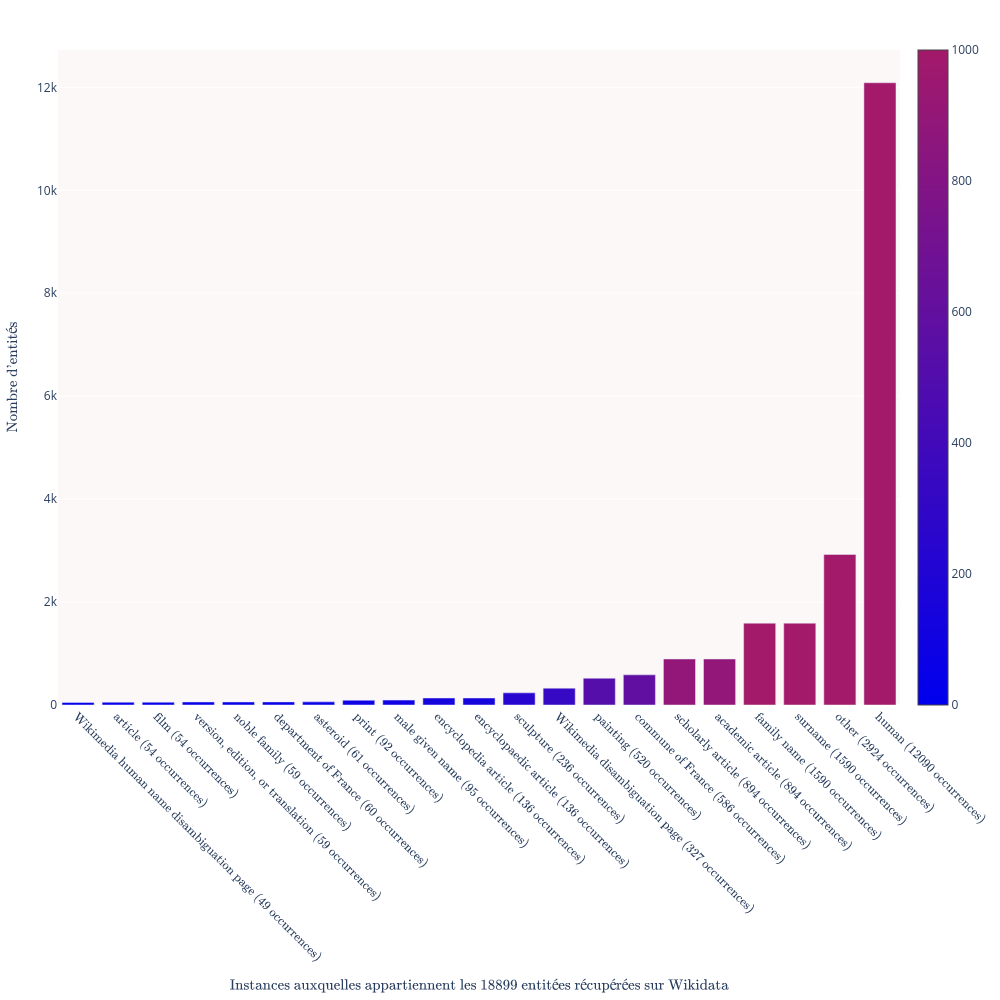
\includegraphics[width=\linewidth]{annexes/fig_wikidata_instances.png}
	\caption \\Occurrences des différentes catégories auxquelles appartiennent les entités \wkd{} liées avec les entrées de catalogues
	\label{appendix:wikidata_instances}
\end{figure}

\begin{figure}
	\centering
	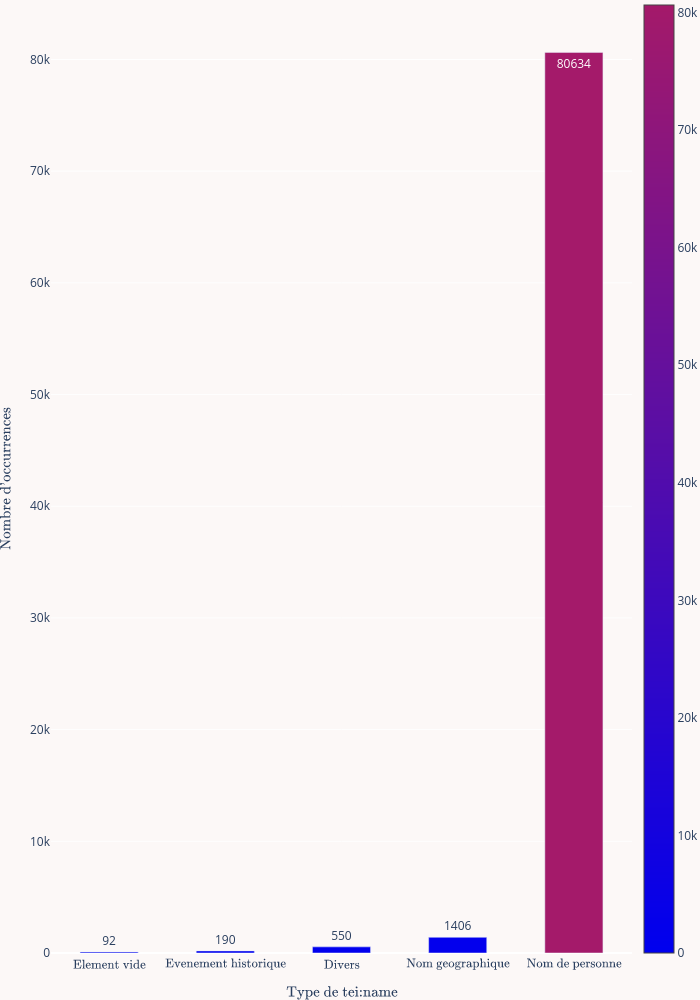
\includegraphics[width=\linewidth]{annexes/fig_teinametypes.png}
	\caption{Répartition des différents types de \tname{}}
	\label{appendix:tnametypes}
\end{figure}

\chapter{Code source et données encodées}
\begin{listing}[p]
	\begin{minted}{python}
functions = {
	"général": "general",
	"maréchal": "marshal",
	"lieutenant": "military",
	"officier": "military",
	"colonel": "military",
	"lieutenant-colonel": "military",
	"commandant": "military",
	"capitaine": "military",  # "less important" military positions
	"roi": "king",
	"empereur": "emperor",
	"president": "president",
	"homme politique": "politician",
	"président de l'assemblée": "politician",
	"orateur": "politician",
	"député": "politician",
	"secrétaire d'état": "politician",
	"sénateur": "politician",
	"écrivain": "writer",
	"auteur": "writer",
	"romancier": "writer",
	"acteur": "actor",
	"actrice": "actress",
	"cantatrice": "singer",
	"chanteur": "singer",
	"chanteuse": "singer",
	"peintre": "painter",
	"sculpteur": "sculptor",
	"statutaire": "sculptor",
	"compositeur": "composer",
	"musicien": "musician",
	"musicienne": "musician",
	"tragédien": "actor",
	"chansonnier": "chansonnier",
	"achitecte": "architect",
	"journaliste": "journalist",
	"inventeur": "inventor",
	"chimiste": "chemist",
	"connétable": "constable",
	"archevêque": "archbishop",
	"évêque": "bishop",
	"docteur": "physicist",
	"médecin": "physicist"
}		
	\end{minted}
	\caption{Table de conversion associant un métier à son équivalent normalisé}
	\label{appendix:convfunction}
\end{listing}

\clearpage
\begin{multipageminted}
	\begin{minted}{python}
dpts = [
	"ain",
	"aisne",
	"allier",
	"basses-alpes",
	"hautes-alpes",
	"alpes-maritimes",
	"annepins",
	"provence",
	"ardèche",
	"ardennes",
	"arriège",
	"arno",
	"aube",
	"aude",
	"aveyron",
	"bouches-de-l'elbe",
	"bouches-de-l'escaut",
	"bouches-de-l'yssel",
	"bpuches-de-la-meuse",
	"bouches-du-rhin",
	"bouches-du-rhône",
	"bouches-du-weser",
	"calvados",
	"cantal",
	"charente",
	"charente-inférieure",
	"cher",
	"corrèze",
	"corse",
	"côte-d'or",
	"côtes-du-nord",
	"creuse",
	"deux-nèthes",
	"deux-sèvres",
	"doire",
	"dordogne",
	"doubs",
	"drôme",
	"dyle",
	"ems-occidental",
	"ems-oriental",
	"ems-supérieur",
	"escaut",
	"eure",
	"eure-et-loir",
	"finistère",
	"forêts",
	"gard",
	"haute-garonne",
	"gers",
	"gironde",
	"hérault",
	"ille-et-villaine",
	"indre",
	"indre-et-loire",
	"isère",
	"jemappes",
	"jura",
	"landes",
	"léman",
	"loire",
	"loir-et-cher",
	"haute-loire",
	"loire-inférieure",
	"loiret",
	"lot",
	"lot-et-garonne",
	"lozère",
	"lys",
	"maine-et-loire",
	"manche",
	"marengo",
	"marne",
	"haute-marne",
	"méditerrannée",
	"mayenne",
	"meurthe",
	"meuse",
	"meuse-inférieure",
	"mont-blanc",
	"mont-tonnerre",
	"montenotte",
	"morbihan",
	"meuse",
	"moselle",
	"nièvre",
	"nord",
	"oise",
	"ombrone",
	"orne",
	"ourte",
	"paris",
	"pas-de-calais",
	"pô",
	"puy-de-dôme",
	"hautes-pyrénées",
	"basses-pyrénées",
	"pyrénées-orientales",
	"haut-rhin",
	"bas-rhin",
	"rhin-et-moselle",
	"rhône",
	"rhône-et-loire",
	"roer",
	"rome",
	"haute-saône",
	"saône-et-loire",
	"sambre-et-meuse",
	"sarre",
	"sarthe",
	"seine",
	"seine-et-marne",
	"seine-et-oise",
	"seine-inférieure",
	"sézia",
	"simplon",
	"deux-sèvres",
	"somme",
	"stura",
	"tarn",
	"tarn-et-garonne",
	"taro",
	"trasimène",
	"var",
	"vaucluse",
	"vendée",
	"vienne",
	"haute-vienne",
	"vosges",
	"yonne",
	"yssel-supérieur",
	"zuyderzée"
]		
	\end{minted}
	\caption{Liste de départements du XIXe~s. pour détecter des informations géographiques}
	\label{appendix:convdpt}
\end{multipageminted}
\clearpage

\begin{listing}[p]
	\begin{minted}{python}
countries = {
	"états-unis d'amérique": "united states of america",
	"etats-unis d'amérique": "united states of america",
	"états unis d'amérique": "united states of america",
	"etats unis d'amerique": "united states of america",
	"états-unis": "united states of america",
	"etats-unis": "united states of america",
	"etats unis": "united states of america",
	"états unis": "united states of america",
	"italie": "italy",
	"grèce": "greece",
	"canada": "canada",
	"chine": "china",
	"haïti": "haiti",
	"tobago": "tobago",
	"brésil": "brasil",
	"burkina-faso": "burkina-faso",
	"cameroun": "cameroun",
	"tchad": "tchad",
	"congo": "congo",
	"gabon": "gabon",
	"guinée": "guinea",
	"côte d'ivoire": "ivory coast",
	"mali": "mali",
	"mauritanie": "mauritania",
	"niger": "niger",
	"sénégal": "senegal",
	"madagascar": "madagascar",
	"seychelles": "seychelles",
	"tanzanie": "tanzania",
	"zanzibar": "zanzibar",
	"liban": "lebanon",
	"syrie": "syria",
	"inde": "india",
	"laos": "laos",
	"viet-nâm": "vietnam"
}	
	\end{minted}
	\caption{Table de conversion pour les pays}
	\label{appendix:convcountry}
\end{listing}

\clearpage
\begin{multipageminted}
	\begin{minted}{python}
colonies = [
	"québec",
	"ontario",
	"saint-pierre-et-miquelon",
	"mississippi",
	"missouri",
	"louisiane",
	"anguilla",
	"antigua",
	"dominique",
	"saint-domingue",
	"guadeloupe",
	"monsterrat",
	"saint-martin",
	"saint-barthélémy",
	"sainte-lucy",
	"saint-vincent-et-les-grenadines",
	"saint-eustache",
	"saint-christophe",
	"martinique"
	"guyane française",
	"guyane",
	"maroc",  # unfortunately the morocco referred to in XIXth century france is a french protectorate
	"algérie",  # same
	"algérie française",  # same
	"tunisie",  # same
	"fezzan",
	"dahomey",
	"haute-volta",
	"oubangui-chari",
	"congo français",
	"moyen-congo",
	"guinée française",
	"soudan français",
	"gorée",
	"tigi",
	"djibouti",
	"cheikh saïd",
	"comores",
	"fort-dauphin",
	"îles maurice",
	"mayotte",
	"la réunion",
	"îles éparses",
	"île amsterdam",
	"île saint-paul",
	"archipel crozet",
	"îles kerguelen",
	"castellorizo",
	"grand-liban",
	"sandjak d'alexandrette",
	"indes françaises",
	"pondichéry",
	"karikal",
	"yanaon",
	"mahé",
	"chanderngor",
	"tonkin",
	"annam",
	"cochinchine",
	"guangzhou wan",
	"shanghai",
	"guangzhou",
	"tianjin",
	"hankou",
	"clipperton",
	"nouvelle-calédonie",
	"polynésie française",
	"vanuatu",
	"nouvelles-hébrides",
	"wallis et futuna"
]
	\end{minted}
	\caption{Liste d'anciennes colonies françaises utilisées pour la détection de motifs}
	\label{appendix:convcolonie}
\end{multipageminted}
\clearpage

\begin{listing}[p]
	\begin{minted}{python}
provinces = [
	"armagnac",
	"île-de-france",
	"berry",
	"orléanais",
	"normandie",
	"languedoc",
	"lyonnais",
	"dauphiné",
	"champagne",
	"aunis",
	"saintonge",
	"poitou",
	"guyenne et gascogne",
	"bourgogne",
	"picardie",
	"anjou",
	"provence",
	"angoumois",
	"bourbonnais",
	"marche",
	"bretagne",
	"maine",
	"touraine",
	"limousin",
	"comté de foix",
	"auvergne",
	"béarn",
	"alsace",
	"artois",
	"roussillon",
	"flandre française et hainaut français",
	"franche-comté",
	"lorraine et trois-évêchés",
	"corse",
	"nivernais",
]
	\end{minted}
	\caption{Liste d'anciennes provinces françaises pour la détection de motifs}
	\label{appendix:convprov}
\end{listing}

\begin{listing}[p]
	\begin{minted}{python}
events = {
	"défense nationale": "government of national defense",
	"defense nationale": "government of national defense",
	"révolution française": "french revolution",
	"revolution francaise": "french revolution",
	"guerre de trente ans": "thirty years' war 1618 1648",
	"guerre de cent ans": "hundred years' war 1337 1453",
	"guerre de sept ans": "seven years war 1756 1763",
	"guerre": "war",
	"insurrection": "war",
	"siège de mayence": "siege of mainz",
	"siège": "siege",
	"commune": "commune",
	"défense": "battle",
	"révolution": "revolution"
}
	\end{minted}
	\caption{Table de conversion pour les évènements historiques}
	\label{appendix:convevt}
\end{listing}

\begin{listing}[p]
	\begin{minted}{python}
status = {
	"empereur": "",
	"impératrice": "",
	"géneral": "general",
	"reine": "queen",
	"roi": "king",
	"princesse": "princess",
	"prince": "prince",
	"archiduchesse": "",
	"archiduc": "",
	"duchesse": "duchess",
	"duc": "duke",
	"famille": "family",
	"seigneur": "",
	"vicomtesse": "",
	"victesse": "",
	"vicomte": "",
	"victe": "",
	"comtesse palatine": "countess palatine",
	"comtesse": "",
	"ctesse": "",
	"comte": "",
	"cte": "",
	"cardinal": "",
	"pape": "pope",
	"lord": "",
	"chevalier": "",
	"marquise": "",
	"marquis": "",
	"sire": "",
	"baronnesse": "",
	"baronne": "",
	"baron": "",
	"abbé": "",
	"madame": "",
	"mme": "",
	"monsieur": "",
	"mr": "",
	"docteur": "",
	"maréchale": "",
	"maréchal": "",
	"mademoiselle": "",
	"melle": "",
	"mlle": "",
	"sir": ""
}
	\end{minted}
	\caption{Liste de colonies pour la détection de motifs}
	\label{appendix:convstatus}
\end{listing}

\begin{listing}[p]
	\begin{minted}{python}
comp_names = {
	"arm ch": "armand-charles",
	"ch m": "charles-marie",
	"ch l f": "charles-louis-françois",
	"f m": "francois-marie",
	"fr emm.": "françois-emmanuel",
	"j ant": "jean-antoine",
	"j f": "jean-francois",
	"j m": "jean-marie",
	"j j": "jean-jacques",
	"j l": "jean-louis",
	"j b": "jean-baptiste",
	"j p": "jean-pierre",
	"j pierre": "jean-pierre",
	"l f": "louis-françois",
	"m f": "marius-felix",
	"franc rené": "francois-rené",
	"m madeleine": "marie-madeleine",
	"ph h": "philippe henri",
	"p aug": "pierre auguste",
	"p alex": "pierre alexandre",
	"p j": "pierre-jean",
	"j sylvain": "jean-sylvain",
	"l ph": "louis-philippe",
	"edm ch": "edmond-charles",
	"ch marie": "charles-marie"
}
	\end{minted}
	\caption{Table de conversion permettant de remplacer un nom abrégé composé par sa version complète}
	\label{appendix:namecomp}
\end{listing}

\begin{listing}[p]
	\begin{minted}{python}
names = {
	"ad": "adam",
	"alex": "alexandre",
	"alph": "alphonse",
	"ant": "antoine",
	"arm": "armand",
	"aug": "auguste",
	"ch": "charles",
	"cl": "claude",
	"dom": "dominique",
	"emm": "emmanuel",
	"ed": "edouard",
	"et": "etienne",
	"ét": "etienne",
	"ferd": "ferdinand",
	"fred": "frederic",
	"fr": "françois",
	"franc": "françois",
	"franç": "françois",
	"fréd": "frédéric",
	"g": "guillaume",
	"guill": "guillaume",
	"gab": "gabriel",
	"jh": "joseph",
	"jacq": "jacques",
	"jos": "joseph",
	"math": "matthieu",
	"nic": "nicolas",
	"ph": "philippe",
	"v": "victor",
	"vr": "victor",
}
	\end{minted}
	\caption{Table de conversion permettant de remplacer un nom abrégé non composé par sa version complète}
	\label{appendix:namesimp}
\end{listing}

\clearpage
\begin{multipageminted}
	\begin{minted}[breakanywhere]{python}
def rgx_abvcomp(nstr):
	"""
	try to extract an abbreviated composed first name. if there is no match, return None
	pattern
	-------
	the patterns in the example below are simplified to keep things readable
	- two strings separated by a "-" or "\s"
	- the first or second string can be a full name ([A-Z][a-z]+)
	or an abbreviation ([A-Z][a-z]*\.)
	- if the strings are separated by "\s", they must be finished by "\."
	(to be sure that we don't capture full names, i.e: "J. Ch."  can be captured,
	but not "Jean Charles")
	- complex names with 3 or more words must have "-" and at least one "\."
	- (\s|$) and (^|\s) are safeguards to avoid matching the end or beginning of another word
	examples
	--------
	matched : M.-Madeleine Pioche de la Vergne  # matched string : M.-Madeleine
	matched : C.-A. de Ferriol  # matched string : C.-A.
	matched : J. F.  # matched string : J. F.
	matched : Jean F.  # matched string : Jean F.
	matched : Jean-F.  # matched string : Jean-F.
	matched : A M  # matched string : A M
	matched : C.-Edm.-G.  # matched string : C.-Edm.-G.
	matched : Charles-Edm.-G.  # matched string : Charles-Edm.-G.
	not matched : Anne M
	not matched : Claude Henri blabla
	not matched : Claude Henri
	:param nstr: the name string used as input
	:return: the matched string if there is a match ; None if there is no match
	"""
	mo = re.search(r"(^|,|\s)[A-ZÀÂÄÈÉÊËÏÔŒÙÛÜŸ][a-zàáâäéèêëíìîïòóôöúùûüøœæç]*"
			+ "\.?-[A-ZÀÂÄÈÉÊËÏÔŒÙÛÜŸ][a-zàáâäéèêëíìîïòóôöúùûüøœæç]*\.(\s|,|$)", nstr) \
		 or re.search(r"(^|,|\s)[A-ZÀÂÄÈÉÊËÏÔŒÙÛÜŸ][a-zàáâäéèêëíìîïòóôöúùûüøœæç]*\."
			+ "-[A-ZÀÂÄÈÉÊËÏÔŒÙÛÜŸ][a-zàáâäéèêëíìîïòóôöúùûüøœæç]*\.?(\s|,|$)", nstr) \
		 or re.search(r"(^|,|\s)[A-ZÀÂÄÈÉÊËÏÔŒÙÛÜŸ]\.?\s"
			+ "[A-ZÀÂÄÈÉÊËÏÔŒÙÛÜŸ][a-zàáâäéèêëíìîïòóôöúùûüøœæç]*\.(\s|,|$)", nstr) \
		 or re.search(r"(^|,|\s)[A-ZÀÂÄÈÉÊËÏÔŒÙÛÜŸ][a-zàáâäéèêëíìîïòóôöúùûüøœæç]*\.?"
		    + "\s[A-ZÀÂÄÈÉÊËÏÔŒÙÛÜŸ]\.(\s|,|$)", nstr) \
		 or re.search(r"(^|,|\s)[A-ZÀÂÄÈÉÊËÏÔŒÙÛÜŸ]\.?\s[A-ZÀÂÄÈÉÊËÏÔŒÙÛÜŸ]\.?(\s|,|$)", nstr) \
		 or re.search(r"([A-ZÀÂÄÈÉÊËÏÔŒÙÛÜŸ]\.){2,}", nstr) \
		 or re.search(r"(^|,|\s)([A-ZÀÂÄÈÉÊËÏÔŒÙÛÜŸ][a-zàáâäéèêëíìîïòóôöúùûüøœæç]*\.?-)+"
			+ "([A-ZÀÂÄÈÉÊËÏÔŒÙÛÜŸ][a-zàáâäéèêëíìîïòóôöúùûüøœæç]*\.)(\s|,|$)", nstr) \
		 or re.search(r"(^|,|\s)([A-ZÀÂÄÈÉÊËÏÔŒÙÛÜŸ][a-zàáâäéèêëíìîïòóôöúùûüøœæç]*\.-)+"
		  	+ "([A-ZÀÂÄÈÉÊËÏÔŒÙÛÜŸ][a-zàáâäéèêëíìîïòóôöúùûüøœæç]*\.?)(\s|,|$)", nstr)
	if mo is not None:
		return mo[0]
	else:
		return None
	\end{minted}
	\caption{Fonction permettant d'identifier et d'extraire un nom abrégé composé}
	\label{appendix:rgxabvcomp}
\end{multipageminted}
\clearpage

\begin{listing}[p]
	\begin{minted}[breakanywhere]{python}
def rgx_abvsimp(nstr):
	"""
	try to extract a "simple" (not composed) abbreviated first name. if there is no match, return None
	pattern
	-------
	a capital letter (possibly followed by a certain number of lowercase letters)
	ended with a dot. (\s|$) and (^|\s) are safeguards to avoid matching the beginning
	end of another word.
	*warning* : it can also capture parts of composed abbreviated names => must be used
	in an if-elif after trying to match a composed abbreviated name
	examples
	--------
	matched : bonjour Ad.  # matched string : Ad.
	matched : J. baronne  # matched string : J.
	matched : J. F.  # matched string : J.
	matched : Jean F.  # matched string : F.
	not matched : A.-M.
	not matched : Anne M
	not matched : Hector
	:param nstr: the name string used as input
	:return:
	"""
	mo = re.search(r"(^|\s)[A-ZÀÂÄÈÉÊËÏÔŒÙÛÜŸ][a-zàáâäéèêëíìîïòóôöúùûüøœæç]*\.(\s|$|,)", nstr)
	if mo is not None:
		return mo[0]
	else:
		return None
	\end{minted}
	\caption{Fonction permettant de repérer et d'extraire un nom abrégé simple}
	\label{appendix:rgxabvsimp}
\end{listing}

\begin{listing}[p]
	\begin{minted}[breakanywhere]{python}
def rgx_complnm(nstr):
	"""
	try to extract a complete name from a string. if there is noœ match, return None
	pattern
	-------
	- an uppercase letter followed by several lowercase letters ;
	- this pattern can be repeated several times, separated by a space or "-"
	- (\s|$) and (^|\s) are safeguards to avoid matching the beginning or end of another word.
	:param nstr: the string from which a name should be extracted
	:return:
	"""
	mo = re.search(r"(^|\s)[A-ZÀÂÄÈÉÊËÏÔŒÙÛÜŸ][a-zàáâäéèêëíìîïòóôöúùûüøœæç]+"
		+ "((\s|-)[A-ZÀÂÄÈÉÊËÏÔŒÙÛÜŸ][a-zàáâäéèêëíìîïòóôöúùûüøœæç]+)*($|\s|,)", nstr)
	if mo is not None:
		return mo[0]
	else:
		return None
	\end{minted}
	\caption{Fonction permettant d'identifier et d'extraire un nom complet non abrégé}
	\label{appendix:rgxfull}
\end{listing}
\pagebreak

\clearpage
\begin{figure}[!htb]
	\begin{subfigure}{\textwidth}
		\begin{minted}{xml}
<item n="264" xml:id="CAT_000327_e264">
	<!-- ... -->
	<name type="author">Spontini (Gaspard)</name>
	<trait>
		<p>célèbre compositeur, auteur de la Vestale, né en 1779, mort en 1851.</p>
	</trait>
	<!-- ... -->
</item>
		\end{minted}
		\subcaption{La source \xmltei{}}
	\end{subfigure}
	\begin{subfigure}{\textwidth}
		\begin{minted}{python}
{
	'fname': 'gaspard ', 
	'lname': 'spontini ', 
	'nobname_sts': '', 
	'status': '', 
	'dates': '1779 1851 ', 
	'function': 'writer', 
	'rebuilt': False
}
		\end{minted}
		\caption{Le dictionnaire d'informations structurées}
	\end{subfigure}
	\begin{subfigure}{\textwidth}
		\begin{lstlisting}
gaspard spontini 1779 1851 writer
gaspard spontini 1851 writer
gaspard spontini 1779 writer
gaspard spontini writer
spontini 1779 1851 writer
spontini 1851 writer
spontini 1779 writer
spontini writer
		\end{lstlisting}
		\caption{Les recherches lancées sur l'\api{} \wkd{}}
	\end{subfigure}
	\caption{De la \tei{} à l'\api{}: document en entrée, informations extraites et chaînes de caractères recherchées}
	\label{code:apipipeline}
\end{figure}
Ci dessus (\ref{code:apipipeline}) sont présentés l'entrée et les données produites lors de l'alignement avec \wkd{}: en premier les données en entrée, ensuite les informations qui en sont extraites et enfin les différentes chaînes de caractères recherchées. Il est à noter que, dans la plupart des cas, seules une ou deux recherches sont faites sur l'\api{} avant d'obtenir un résultat; ici, huit chaînes différentes ont été construites et recherchées, ce qui représente l'intégralité de l'algorithme.
\clearpage

\chapter{Images}
\begin{figure}[p]
	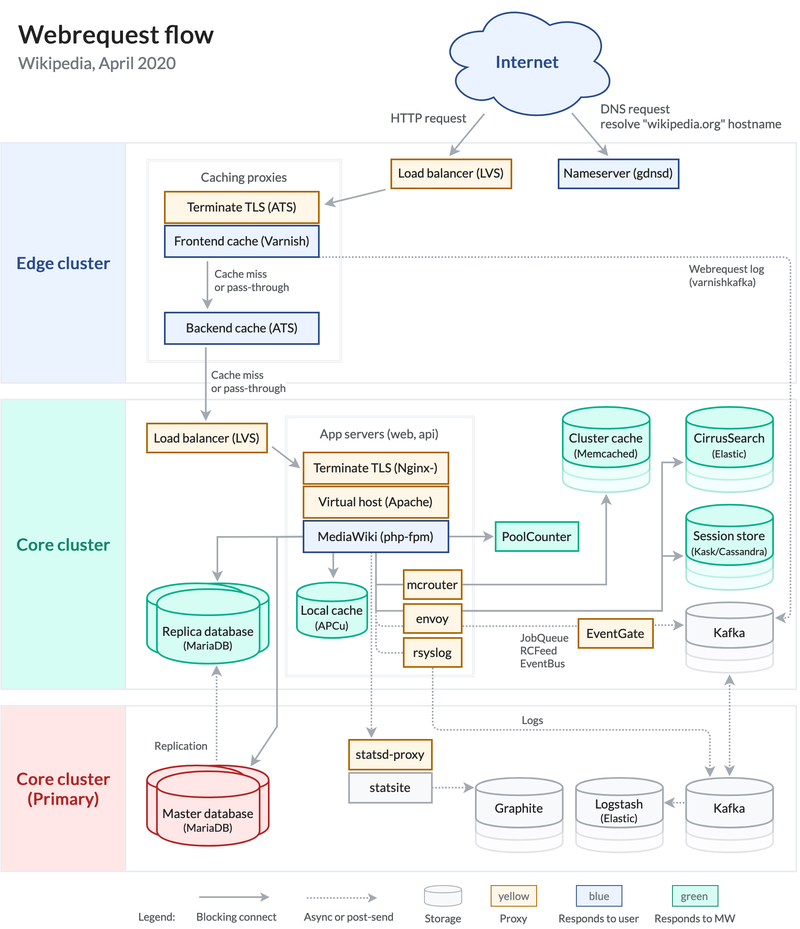
\includegraphics[width=\textwidth]{annexes/wikimedia_db_2020.png}
	\caption{L'architecture des bases de données de la \textit{Wikimedia Foundation} (schéma réalisé par Timo Tijhof en 2020, disponible dans le domaine public avec la licence Creative Commons CC0.1.0 Universal Public Domain License)}
	\label{appendix:wikimedia_db}
\end{figure}	
	
	
	
\end{document}